\documentclass[onecolumn, 12pt]{book}

%----------------------------------------------- debut usepackage -------------------------------------------------------------
\usepackage[latin1]{inputenc}   
%\usepackage[utf8]{inputenc}
\usepackage{amsmath}
\usepackage{algorithm,algorithmic} 
%\usepackage[T1]{fontenc}
%\usepackage[francais]{babel}     
\usepackage{layout}    
\usepackage[top=2cm, bottom=2cm, left=2cm, right=2cm]{geometry} 
\geometry{
	left=16mm,
	top=30mm,
	right=16mm,
	bottom=30mm
}
\usepackage{setspace}
\usepackage{soul}
\usepackage{color} 
\usepackage{verbatim}
\usepackage{moreverb}
\usepackage{listings}
\usepackage{url}
\usepackage{graphicx}
%\usepackage[outdir=./]{epstopdf}
\usepackage[outdir=./images_fusionChapitres/]{epstopdf}
\usepackage{caption}
\usepackage{setspace}
\usepackage{enumitem} 
\usepackage{amsthm} % ajouter pour environnement proof
\usepackage{placeins}
\usepackage{multirow}

\usepackage{titlesec} 
\usepackage{hyperref}
\usepackage{pdfpages}

%%%% page de garde et abstract
\usepackage{helvet}
\usepackage{array}
\usepackage{xcolor}
\definecolor{bordeau}{rgb}{0.3515625,0,0.234375}
\usepackage[absolute,overlay]{textpos}
\usepackage{multicol}
\setlength{\columnseprule}{0pt}
\setlength\columnsep{10pt}
%%%% page de garde et abstract 

%%% ------ nouveau import package ------------
%%%%----- handle titlesec : generate problem ------
%% solution 1 : update package titlesec 
%%%-------- link : https://tex.stackexchange.com/questions/299969/titlesec-loss-of-section-numbering-with-the-new-update-2016-03-15
%% solution 2 : below
\usepackage{etoolbox}

\makeatletter
\patchcmd{\ttlh@hang}{\parindent\z@}{\parindent\z@\leavevmode}{}{}
\patchcmd{\ttlh@hang}{\noindent}{}{}{}
\makeatother
%%%%----- headle titlesec : generate problem ------

\let\proof\relax
\let\endproof\relax
\usepackage{amsmath, amsthm, amssymb}
\usepackage{amsfonts}
%-------------------------------------------------- fin usepackage -------------------------------------------------------------

% --------------------------------------------- new commands ----------------------------------------------------------------
\renewcommand{\chaptername}{Chapitre}
\renewcommand{\contentsname}{Table des Mati\`eres}
\renewcommand{\bibname}{Bibliographie}
\renewcommand{\tablename}{Tableau}
%\renewcommand{\figurename}{Fig}
\renewcommand{\listfigurename}{Liste des figures}
\renewcommand{\listtablename}{Liste des Tableaux}
\renewcommand{\listalgorithmname}{Liste des Algorithmes}
%\renewcommand{\thealgorithm}{\arabic{chapter}.\arabic{algorithm}} 

%%%%%-------------- redefine part, section, subsection , subsubsection, subsubsubsection ------ 
\titleclass{\subsubsubsection}{straight}[\subsection]

\newcounter{subsubsubsection}[subsubsection]
\renewcommand\thesubsubsubsection{\thesubsubsection.\arabic{subsubsubsection}}
\renewcommand\theparagraph{\thesubsubsubsection.\arabic{paragraph}} % optional; useful if paragraphs are to be numbered

\titleformat{\subsubsubsection}
  {\normalfont\normalsize\bfseries}{\thesubsubsubsection}{1em}{}
\titlespacing*{\subsubsubsection}
{0pt}{3.25ex plus 1ex minus .2ex}{1.5ex plus .2ex}

\makeatletter
\renewcommand\paragraph{\@startsection{paragraph}{5}{\z@}%
  {3.25ex \@plus1ex \@minus.2ex}%
  {-1em}%
  {\normalfont\normalsize\bfseries}}
\renewcommand\subparagraph{\@startsection{subparagraph}{6}{\parindent}%
  {3.25ex \@plus1ex \@minus .2ex}%
  {-1em}%
  {\normalfont\normalsize\bfseries}}
\def\toclevel@subsubsubsection{4}
\def\toclevel@paragraph{5}
\def\toclevel@paragraph{6}
\def\l@subsubsubsection{\@dottedtocline{4}{7em}{4em}}
\def\l@paragraph{\@dottedtocline{5}{10em}{5em}}
\def\l@subparagraph{\@dottedtocline{6}{14em}{6em}}
\makeatother

\setcounter{secnumdepth}{7}
\setcounter{tocdepth}{7}
%%%%%-------------- redefine part, section, subsection , subsubsection, subsubsubsection ------




\newcommand{\overbar}[1]{\mkern 1.5mu\overline{\mkern-1.5mu#1\mkern-1.5mu}\mkern 1.5mu}
 %---- add name algorithm 
 \makeatletter
\renewcommand{\ALG@name}{Algorithme}
\makeatother
% ----------------------------------- new commands --------------------------------------------------------------------------

 %---------- definitions ------------------
\def\R{\mbox{I\hspace{-.15em}R}}
\def\N{\mbox{I\hspace{-.15em}N}}
\def\Z{\mbox{I\hspace{-.15em}Z}}
\def\Q{\mbox{I\hspace{-.15em}Q}}

\newtheorem{definition}{D\'efinition}
\newtheorem{theorem}{Th\'eor\`eme}
\newtheorem{property}{Propri\'et\'e}
\newtheorem{claim}[theorem]{Claim}
\newtheorem{proposition}[theorem]{Proposition}
\newtheorem{lemma}[theorem]{Lemme}
\newtheorem{corollary}[theorem]{Corollaire}
\newtheorem{conjecture}[theorem]{Conjecture}
\newtheorem{observation}{Observation}
\newtheorem{example}{Exemple}
\newtheorem{remark}{Remarque}
\newtheorem{Proof}{Preuve}
%---------- definitions ------------------
 
% \title{Mod\`ele de Donn\'ees}
% \author{Willy Ehounou}
 %\date{01/06/15}
%\title{Algorithme de graphes pour la d\'ecouverte de la topologie d'un r\'eseau \'energ\'etique par la connaissance de ses flots}
\title{}
\author{}
\date{}
%\author{Wilfried Ehounou}
%\date{\oldstylenums{1875}} 


% -------- chemin images et graphiques
\graphicspath{
%{/home/willy/Documents/latexDoc/redaction/fusion_fichiers_v2/images_fusionChapitres/}
{./images_fusionChapitres/}
{./pageDeGarde/}
}

\makeatletter
%% -------------------------------------- repertoire des fichiers de chaque chapitre -----------------------------
\def\input@path{
{./introductionGenerale/}
{./reseauFlotsMesures/}
{./timeSeries/}
{./linegraphes/}
{./simulation/}
{./conclusionGenerale/}
{./pageDeGarde/}
{./remerciements/}
}
%% -------------------------------------- repertoire des fichiers de chaque chapitre -----------------------------
\makeatother

\setlength{\belowcaptionskip}{-5pt}

%% ------------------------------------- page de Garde, abstract : informations ------------------------------------
%%%%%%%%%%%%%%%%%%%%%%%%%%%%%%%%%%%%%%%%%%%%%%%%%%%%%%%%%%%%%%%%%%%%%%%%%%%%%%%%%%%%%%%%%%%%%%%%%%%%%%%%%%%%%%%%%%%%%%%%%%%%%%%%%%%%%%%%%%%%%%%%%%%%%%%%%%%%%%%%%%%%%%%
%%%%%%%%%%%%%%%%%%%%%%%%%%%%%%%%%%%%%%%%%%%%%%%%%%%%%%%%%%%%%%%%%%%%%%%%%%%%%%%%%%%%%%%%%%%%%%%%%%%%%%%%%%%%%%%%%%%%%%%%%%%%%%%%%%%%%%%%%%%%%%%%%%%%%%%%%%%%%%%%%%%%%%%
%%% Modèle pour la 1ère de couverture des thèses préparées à l'Université Paris-Saclay, basé sur le modèle produit par Guillaume BRIGOT / Template for back cover of thesis made at Université Paris-Saclay, based on the template made by Guillaume BRIGOT
%%% Mis à jour par Aurélien ARNOUX (École polytechnique)/ Updated by Aurélien ARNOUX (École polytechnique)
%%% Les instructions concernant chaque donnée à remplir sont données en bloc de commentaire / Rules to fill this file are given in comment blocks
%%% ATTENTION Ces informations doivent tenir sur une seule page une fois compilées / WARNING These informations must contain in no more than one page once compiled
%%%%%%%%%%%%%%%%%%%%%%%%%%%%%%%%%%%%%%%%%%%%%%%%%%%%%%%%%%%%%%%%%%%%%%%%%%%%%%%%%%%%%%%%%%%%%%%%%%%%%%%%%%%%%%%%%%%%%%%%%%%%%%%%%%%%%%%%%%%%%%%%%%%%%%%%%%%%%%%%%%%%%%%
%%% Version du 05 Avril 2018
%%%%%%%%%%%%%%%%%%%%%%%%%%%%%%%%%%%%%%%%%%%%%%%%%%%%%%%%%%%%%%%%%%%%%%%%%%%%%%%%%%%%%%%%%%%%%%%%%%%%%%%%%%%%%%%%%%%%%%%%%%%%%%%%%%%%%%%%%%%%%%%%%%%%%%%%%%%%%%%%%%%%%%%

%\documentclass[a4paper]{book}
%\usepackage[utf8]{inputenc}
%\usepackage{helvet}
%\renewcommand{\familydefault}{\sfdefault}
%\usepackage{geometry}
%\geometry{
%	left=16mm,
%	top=30mm,
%	right=16mm,
%	bottom=30mm
%}
%\usepackage{xcolor}
%\definecolor{bordeau}{rgb}{0.3515625,0,0.234375}
%\usepackage[absolute,overlay]{textpos}
%\usepackage{graphicx}
%\usepackage{lipsum}
%\usepackage{hyperref}
%\usepackage{array}
%\usepackage{caption}
%\usepackage{multicol}
%\setlength{\columnseprule}{0pt}
%\setlength\columnsep{10pt}
%%\usepackage[french]{babel}

\label{form}
%%%%%%%%%%%%%%%%%%%%%%%%%%%%%%%%%%%%%%%%%%%%%%%%%%%%%%%%%%%%%%%%%%%%%%%%%%%%%%%%%%%%%%%%%%%%%%%%%%%%%%%%%%%%%%%%%%%%%%%%%%%%%%%%%%%%%%%%%%%%%%%%%%%%%%%%%%%%%%%%%%%%%%%
%%%%%%%%%%%%%%%%%%%%%%%%%%%%%%%%%%%%%%%%%%%%%%%%%%%%%%%%%%%%%%%%%%%%%%%%%%%%%%%%%%%%%%%%%%%%%%%%%%%%%%%%%%%%%%%%%%%%%%%%%%%%%%%%%%%%%%%%%%%%%%%%%%%%%%%%%%%%%%%%%%%%%%%
%%% Formulaire / Form
%%% Remplacer les paramètres des \newcommand par les informations demandées / Replace \newcommand parameters by asked informations
%%%%%%%%%%%%%%%%%%%%%%%%%%%%%%%%%%%%%%%%%%%%%%%%%%%%%%%%%%%%%%%%%%%%%%%%%%%%%%%%%%%%%%%%%%%%%%%%%%%%%%%%%%%%%%%%%%%%%%%%%%%%%%%%%%%%%%%%%%%%%%%%%%%%%%%%%%%%%%%%%%%%%%%
%%%%%%%%%%%%%%%%%%%%%%%%%%%%%%%%%%%%%%%%%%%%%%%%%%%%%%%%%%%%%%%%%%%%%%%%%%%%%%%%%%%%%%%%%%%%%%%%%%%%%%%%%%%%%%%%%%%%%%%%%%%%%%%%%%%%%%%%%%%%%%%%%%%%%%%%%%%%%%%%%%%%%%%


\newcommand{\PhDTitle}{Algorithme de graphes pour la d\'ecouverte de la topologie d'un r\'eseau \'energ\'etique par la connaissance de ses flots} 	%% Titre de la thèse / Thesis title
\newcommand{\PhDname}{Wilfried Joseph EHOUNOU} 															%% Civilité, nom et prénom /  Civility, first name and name 
\newcommand{\NNT}{20XXSACLXXXX} 															%% Numéro National de Thèse (donnée par la bibliothèque à la suite du 1er dépôt)/ National Thesis Number (given by the Library after the first deposit)

\newcommand{\ecodoctitle}{Sciences et technologies de l'information et de la communication (STIC)} 													%% Nom de l'ED. Voir site de l'Université Paris-Saclay / Full name of Doctoral School. See Université Paris-Saclay website
\newcommand{\ecodocacro}{STIC}																%% Sigle de l'ED. Voir site de l'Université Paris-Saclay / Acronym of the Doctoral School. See Université Paris-Saclay website
\newcommand{\ecodocnum}{000} 																%% Numéro de l'école doctorale / Doctoral School number
\newcommand{\PhDspeciality}{voir sp\'ecialit\'es par l'ED} 										%% Spécialité de doctorat / Speciality 
\newcommand{\PhDworkingplace}{Universit\'e de Versailles-Saint-Quentin-en-Yvelines } 										%% Établissement de préparation / PhD working place : l'Université Paris-Sud, l'Université de Versailles-Saint-Quentin-en-Yvelines, l'Université d'Evry-Val-d'Essonne, l'Institut des sciences et industries du vivant et de l'environnement (AgroParisTech), CentraleSupélec,l'Ecole normale supérieure de Cachan, l'Ecole Polytechnique, l'Ecole nationale supérieure de techniques avancées, l'Ecole nationale de la statistique et de l’administration économique, HEC Paris, l'Institut d'optique théorique et appliquée, Télécom ParisTech, Télécom SudParis   
\newcommand{\defenseplace}{Versailles} 											%% Ville de soutenance / Place of defense
\newcommand{\defensedate}{/09/2018} 															%% Date de soutenance / Date of defense

%%% Établissement / Institution
%%% Si la thèse a été produite dans le cadre d'une co-tutelle, commenter la partie "Pas de co-tutelle" et décommenter la partie "Co-tutelle" / If the thesis has been prepared in guardianship, comment the part "Pas de co-tutelle" and uncomment the part "Co-tutelle"

	%%%%%%%%%%%%%%%%%%%%%%%%%
	%%% Pas de co-tutelle %%%
	%%%%%%%%%%%%%%%%%%%%%%%%%

%\newcommand{\logoEtt}{blank}																%% NE PAS MODIFIER / DO NOT MODIFY
%\newcommand{\vpostt}{0.1} 																	%% NE PAS MODIFIER / DO NOT MODIFY
%\newcommand{\hpostt}{6}																		%% NE PAS MODIFIER / DO NOT MODIFY
%\newcommand{\logoEt}{etab} 																	%% Logo de l'établissement de soutenance. Indiquer le sigle / Institution logo. Indicate the acronym : AGRO, CENTSUP, ENS, ENSAE, ENSTA, HEC, IOGS, TPT, TSP, UEVE, UPSUD, UVSQ, X 
%\newcommand{\vpos}{0.1}																		%% À modifier au besoin pour aligner le logo verticalement / If needed, modify to align logo vertilcally
%\newcommand{\hpos}{11}																		%% À modifier au besoin pour aligner le logo horizontalement / If needed, modify to align logo horizontaly

		%%%%%%%%%%%%%%%%%%
		%%% Co-tutelle %%%
		%%%%%%%%%%%%%%%%%%

\newcommand{\logoEt}{UVSQ} 																%% Logo de l'université partenaire. Placer le fichier .png dans le répertoire '/media/etab' et indiquer le nom du fichier sans l'extension / Logo of partner university. Place the .png file in the directory '/media/etab' and point the file name without the extension
\newcommand{\vpos}{0.1}																	%% À modifier au besoin pour aligner les logos verticalement / If needed, modify to align logos vertilcally
\newcommand{\hpos}{11}																		%% À modifier au besoin pour aligner les logos horizontalement / If needed, modify to align logos horizontaly
\newcommand{\logoEtt}{UVSQ}  																%% Logo de l'établissement de soutenance. Le nom du fichier correspond au sigle de l'établissement /  Institution logo. Filename correspond to institution acronym : AGRO, CENTSUP, ENS, ENSAE, ENSTA, HEC, IOGS, TPT, TSP, UEVE, UPSUD, UVSQ, X 
\newcommand{\vpostt}{0.1} 																	%% À modifier au besoin pour aligner les logos verticalement / If needed, modify to align logos vertilcally
\newcommand{\hpostt}{6}																	%% À modifier au besoin pour aligner les logos horizontalement / If needed, modify to align logos horizontaly


%%% JURY

% Lors du premier dépôt de la thèse le nom du président n’est pas connu, le choix du président se fait par les membres du Jury juste avant la soutenance. La précision est apportée sur la couverture lors du second dépôt / Choice of the jury's president is made during the defense. Thus, it must be specified only for the second file deposition in ADUM.
% Tous les membres du juty listés doivent avoir été présents lors de la soutenance / All the jury members listed here must have been present during the defense.

%%% Membre n°1 (Président) / Member n°1 (President)
\newcommand{\jurynameA}{Christian LAFOREST}
\newcommand{\juryadressA}{Prof\'esseur, Universit\'e Clermont Auvergne (LIMOS-ISIMA)}
\newcommand{\juryroleA}{Pr\'esident}

%%% Membre n°2 (Rapporteur) / Member n°2 (President)
\newcommand{\jurynameB}{Pascal BERTHOM\'E}
\newcommand{\juryadressB}{Prof\'esseur, Universit\'e Orl\'eans (LIFO)}
\newcommand{\juryroleB}{Rapporteur}

%%% Membre n°3 (Rapporteur) / Member n°3 (President)
\newcommand{\jurynameC}{Daniele GARDY}
\newcommand{\juryadressC}{Professeur, Universit\'e de Versailles (DAVID)}
\newcommand{\juryroleC}{Rapporteur}

%%% Membre n°4 (Examinateur) / Member n°4 (President)
\newcommand{\jurynameD}{Pr\'enom Nom}
\newcommand{\juryadressD}{Statut, \'Etablissement (Unit\'e de recherche)}
\newcommand{\juryroleD}{Examinateur}

%%% Membre n°5 (Directeur de thèse) / Member n°5 (Thesis supervisor)
\newcommand{\jurynameE}{ Dominique BARTH}
\newcommand{\juryadressE}{Professeur, Universit\'e de Versailles (DAVID)}
\newcommand{\juryroleE}{Directeur de th\`ese}

%%% Membre n°6 (Co-directeur de thèse) / Member n°6 (Thesis co-supervisor)
\newcommand{\jurynameF}{Arnaud DE MOISSAC}
\newcommand{\juryadressF}{Ing\'enieur, DCBRAIN}
\newcommand{\juryroleF}{Co-directeur de th\`ese}

%%% Membre n°7 (Invité) / Member n°7 (Guest)
\newcommand{\jurynameG}{Sandrine VIAL}
\newcommand{\juryadressG}{Maitre de conf\'erences, Universit\'e de Versailles (DAVID)}
\newcommand{\juryroleG}{Invit\'e}

%%% Membre n°8 (Invité) / Member n°8 (Guest)
\newcommand{\jurynameH}{Pr\'enom Nom}
\newcommand{\juryadressH}{Statut, \'Etablissement (Unit\'e de recherche)}
\newcommand{\juryroleH}{Invit\'e}

%% Il est possible d'ajouter des membres supplémentaires selon le même modèle / More jury members can be added according to the same model

\label{layout}
%%%%%%%%%%%%%%%%%%%%%%%%%%%%%%%%%%%%%%%%%%%%%%%%%%%%%%%%%%%%%%%%%%%%%%%%%%%%%%%%%%%%%%%%%%%%%%%%%%%%%%%%%%%%%%%%%%%%%%%%%%%%%%%%%%%%%%%%%%%%%%%%%%%%%%%%%%%%%%%%%%%%%%%
%%%%%%%%%%%%%%%%%%%%%%%%%%%%%%%%%%%%%%%%%%%%%%%%%%%%%%%%%%%%%%%%%%%%%%%%%%%%%%%%%%%%%%%%%%%%%%%%%%%%%%%%%%%%%%%%%%%%%%%%%%%%%%%%%%%%%%%%%%%%%%%%%%%%%%%%%%%%%%%%%%%%%%%
%%% Mise en page / Page layout      
%%% NE RIEN MODIFIER EXCEPTÉ LA PARTIE CONCERNANT LE JURY (voir \label{jury}) SI BESOIN / DO NOT MODIFY EXCEPT SECTION CONCERNING JURY (see \label{jury}) IF NEEDED
%%%%%%%%%%%%%%%%%%%%%%%%%%%%%%%%%%%%%%%%%%%%%%%%%%%%%%%%%%%%%%%%%%%%%%%%%%%%%%%%%%%%%%%%%%%%%%%%%%%%%%%%%%%%%%%%%%%%%%%%%%%%%%%%%%%%%%%%%%%%%%%%%%%%%%%%%%%%%%%%%%%%%%%
%%%%%%%%%%%%%%%%%%%%%%%%%%%%%%%%%%%%%%%%%%%%%%%%%%%%%%%%%%%%%%%%%%%%%%%%%%%%%%%%%%%%%%%%%%%%%%%%%%%%%%%%%%%%%%%%%%%%%%%%%%%%%%%%%%%%%%%%%%%%%%%%%%%%%%%%%%%%%%%%%%%%%%%

% Méta-données du PDF / PDF meta-datas
\hypersetup{
	pdfauthor={\PhDname},
	pdfsubject={Manuscrit de th\`ese de doctorat},
	pdftitle={\PhDTitle},
}
   % --------------> ne sert plus a rien
%% -------------------------------------- page de Garde, abstract : informations -----------------------------------

\begin{document}

	% --------- metadonnees du pdf
	\hypersetup{
		pdfauthor={Wilfried Joseph EHOUNOU},
		pdftitle={Algorithme de graphes pour la d\'ecouverte de la topologie d'un r\'eseau \'energ\'etique par la connaissance de ses flots},
		pdfsubject={ th\`ese de doctorat},
		pdfkeywords={Graphes, s\'eries temporelles, similarit\'e, line-graphes, cliques, d\'ecouverte de topologie}
	}
	% --------- metadonnees du pdf
	%---- plan -----
%	\input@path{planBis}

	% ------ page de garde, abstract : execution -------- 
	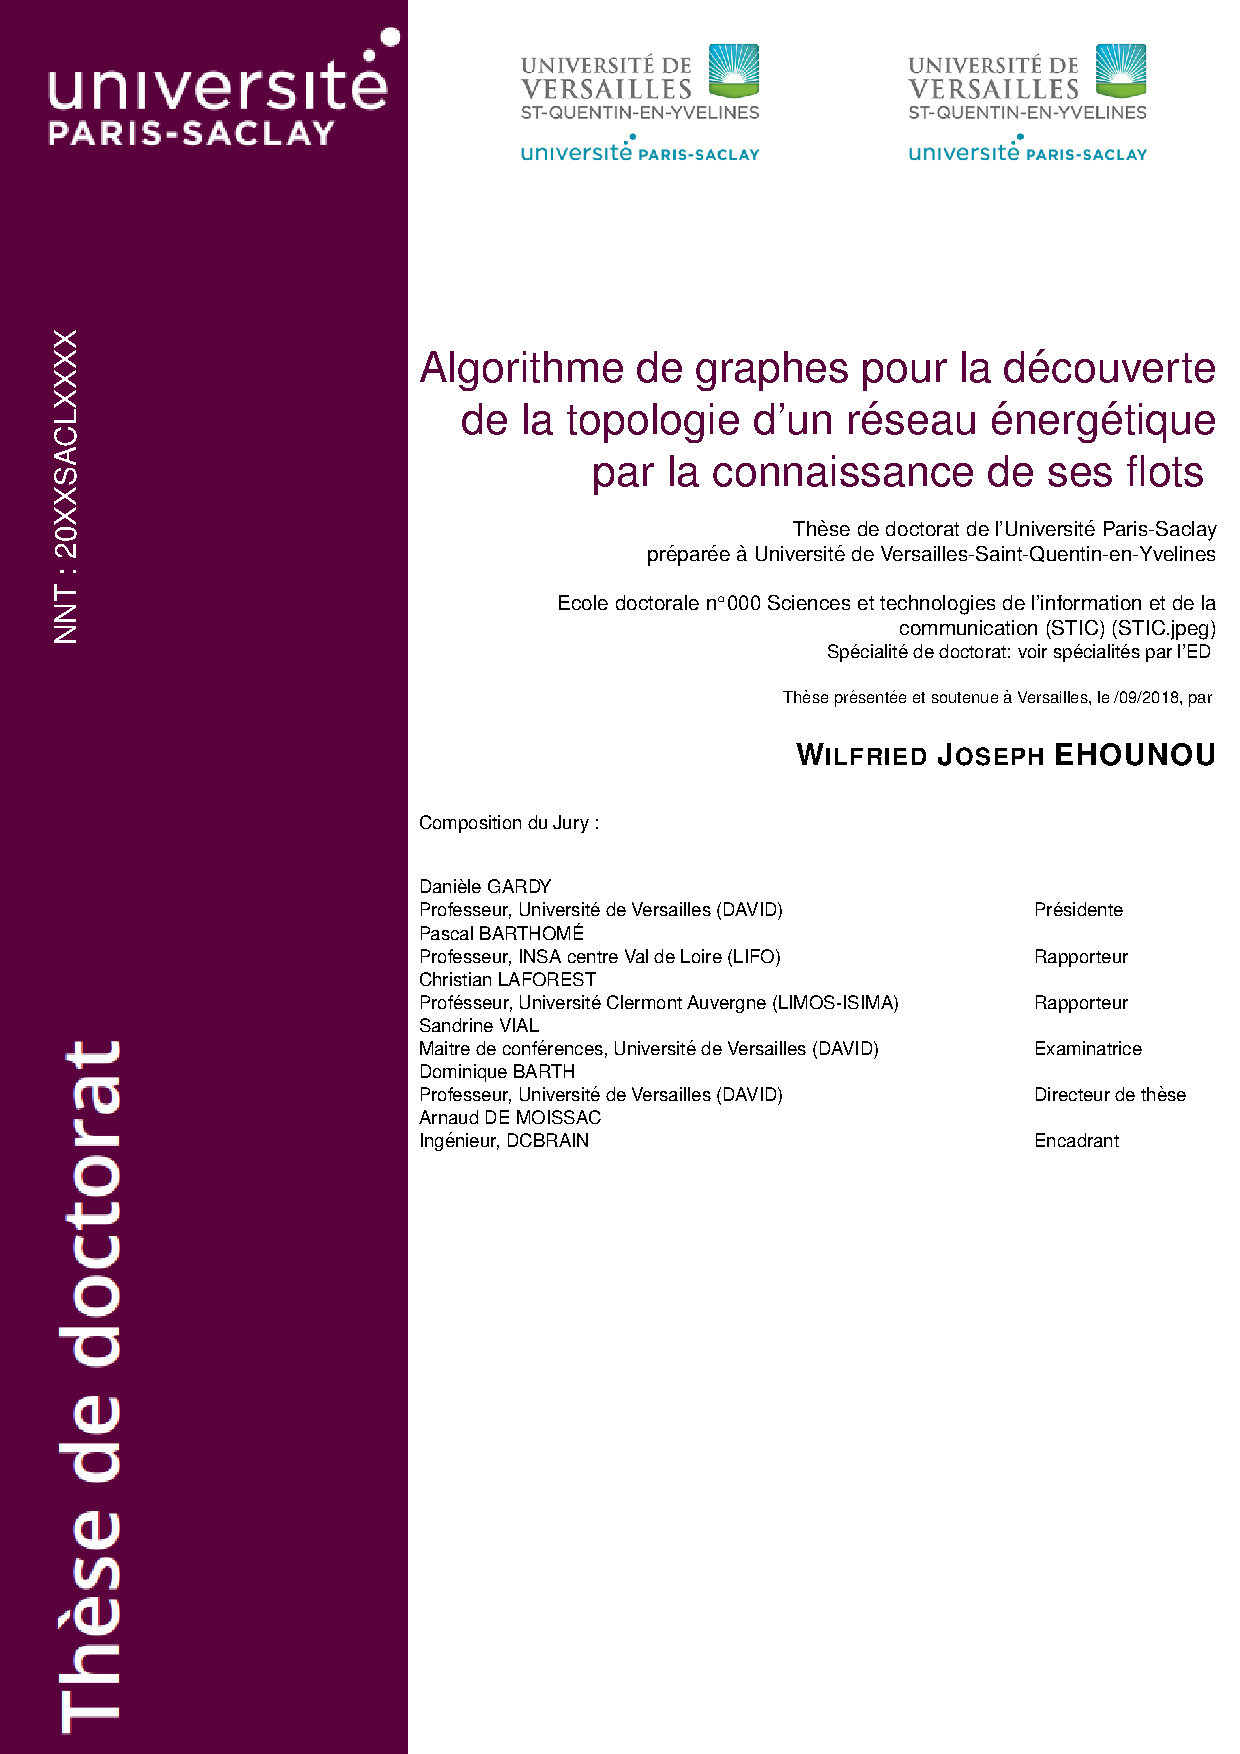
\includepdf[pages={1}]{pageDeGarde_these.pdf}
	\includepdf[pages={1}]{abstract_these.pdf}
	% ------ page de garde, abstract : execution -------- 
	\maketitle
	
	%---- Remerciements
	{\setstretch{1.10}
	\section*{Remerciements}
		

Par ces mots s'ach\`eve la r\'edaction de ce manuscrit.
Je voudrais apporter ma reconnaissance \`a toutes ces personnes qui m'ont accompagn\'ees durant cette p\'eriode en particulier \`a ma famille, aux coll\`egues de DCbrain SAS et aux membres de l'\'equipe DAVID.
\newline 

Un grand merci \`a ma famille pour leur immense soutien. Ils ont \'et\'e patients, compr\'ehensifs et encourageants. Je pense \`a mon p\`ere pour ses encouragements, ma m\`ere pour son reconfort, ma tante F\'elicit\'e pour ses conseils et son hospitalit\'e, mes fr\`eres et soeurs Grace, Prisca, Serge, Maruis, Ismael et Erven. 
\newline
La rencontre de ces personnes a \'et\'e d\'ecisive dans mes choix de vie. 
Mario de son Petionville, merci pour tes conseils \'eclair\'es de la vie.
Dimitri l'\'electrochoc de mon quotidien, merci pour ta vision optimiste. 
Alice merci pour les relectures, tu m'as \'et\'e d'une grande aide.
Cher Henri-Joel, l'ami qui est devenu un fr\`ere, merci d'avoir cru j'y suis arriv\'e. Je t'\'ecouterai plus souvent.   
Adrienne merci pour ses pri\`eres et C\'ecile pour son amour.
\newline

% dcbrain
De Earthgrid \`a DCbrain SAS, l'aventure a d\'ebut\'e par un stage. De $3$ personnes au d\'ebut, elle est devenue une startup de dimension nationale sous la direction des bretons Arnaud et Fran{\c c}ois. 
Arnaud, je retiens de toi ton esprit de management et aussi ta mani\`ere de simplifier un probl\`eme.
Fran{\c c}ois, je retiens  de toi ton  coup de main sur les graphes et ses astuces de programmation.
\`A Maxime, merci pour son assistance et ses conseils en python pour l'impl\'ementation des algorithmes.
Et Damien pour son aide et ses explications sur les s\'eries temporelles.
\newline

%labo
Je voudrai particuli\`erement exprimer ma gratitude \`a  mon encadreur Dominique. Ses d\'ecisions, ses recommendations et sa disponibilit\'e sont le fruit de ce manuscrit. 
Vous n'\^etes pas un professeur pour rien.
\newline

% autres 
A TOUS CEUX QUE JE N'AI PAS CIT\'ES.
Le silence n'est pas synonyme d'oubli; mes pens\'ees vont vers vous ;
\newline

L'enseignement que je retiens de ce travail : \newline
{\em Tout est possible \`a condition de faire le premier pas et de ne pas baisser les bras.}
	
	}

	\tableofcontents
	% ------- listes de figures et tableau et algorithmes
	\listofalgorithms
	\listoffigures
	\listoftables
	
	\onehalfspacing
	%---- introduction
	\chapter{Introduction G\'en\'erale}

Un r\'eseau de distribution \'energ\'etique est un ensemble d'\'equipements \'energ\'etiques interconnect\'es permettant d'ach\'eminer l'\'energie des centres de production aux consommateurs. 
Le r\'eseau est compos\'e d'une infrastructure de transport et d'une infrastructure de distribution de l'\'energie. Ces infrastructures sont sp\'ecifiques \`a l'\'energie et sont g\'er\'ees chacune par un gestionnaire de r\'eseau ou Distribution Source Operator. Son r\^ole est de maintenir la continuit\'e et la qualit\'e de l'approvisionnement physique des clients c'est-\`a-dire assurer l'entretien et le d\'eveloppement du r\'eseau. 
En effet, le gestionnaire de transport achemine, au niveau national, l'\'energie depuis son lieu de production \`a son lieu de consommation \`a travers le r\'eseau de distribution. Quant au gestionnaire de distribution, il distribue l'\'energie aux consommateurs au niveau r\'egional.
\newline

Un exemple de r\'eseau \'energ\'etique g\'er\'e localement par un gestionnaire de r\'eseau est un datacenter. Le datacenter a la particularit\'e de contenir un r\'eseau thermique, \'electrique et informatique. Le r\'eseau \'electrique alimente les \'equipements des autres r\'eseaux. La connaissance de son infrastructure est indispensable pour le gestionnaire afin
de fournir  la puissance n\'ecessaire au fonctionnement d'un \'equipement et 
 d'\'eviter les surco\^uts de production d'\'electricit\'e parce que l'\'electricit\'e ne se stocke pas.
Pour ce faire, 
%les consommations dans le temps des \'equipements du r\'eseau \'electrique sont coll\'ect\'ees 
des sondes sont install\'ees dans le r\'eseau \'electrique afin de collecter les consommations des \'equipements dans le temps. Les mesures temporelles des consommations sont int\'egr\'ees dans un outil de supervision de ce r\'eseau. Cet outil permet d'avoir l'\'etat de tous les \'equipements \`a un instant donn\'ee, de connaitre la topologie de fonctionnement du r\'eseau et aussi la topologie g\'en\'erale du r\'eseau c'est-\`a-dire l'ensemble des \'equipements arr\^et\'es et en fonctionnement.
\newline

Malheureusement,  l'\'etat du r\'eseau affich\'e par l'outil de supervision est souvent \'erron\'e. 
En effet,  les sondes de certains \'equipements pr\'esentes dans le r\'eseau physique ne sont pas r\'epertori\'ees dans la base de donn\'ees de l'outil et leurs mesures ne figurent nulle part dans l'outil de supervision. Cela donne l'impression que ces \'equipements sont en panne et  les \'equipements rattach\'es \`a ces derniers sont aliment\'es par d'autres \'equipements qui fonctionnent en surcapacit\'e.  
En outre, les sondes de certains \'equipements sont interchang\'ees avec d'autres. Les puissances sont remplac\'ees par des intensit\'es et aussi la puissance d'un \'equipement est remplac\'ee par celle  un autre \'equipement. Ces erreurs humaines impliquent le non respect de la loi de conservation des noeuds et aussi une maintenance complexe  parce que nous ignorons les sondes interchang\'ees.
%Enfin, 
Ces probl\`emes proviennent d'une faible communication  entre les diff\'erents m\'etiers dans le datacenter et aussi de la mise \`a jour \'erron\'ee ou tardive des maintenances dans la base de donn\'ees de l'outil. 
Ceux-ci entrainent  des pr\'evisions \'elev\'ees de consommation \'electriques, des co\^uts de maintenances exorbitants et enfin que la topologie connue n'est pas la topologie r\'eelle.
\newline

Afin de r\'eduire les erreurs humaines dans la d\'ecouverte du r\'eseau, nous proposons des m\'ethodes pour d\'eterminer la topologie du r\'eseau \'electrique en se basant uniquement sur les mesures temporelles collect\'ees. 
Des travaux similaires de d\'ecouverte de topologie ont \'et\'e r\'ealis\'es par l'entreprise {\em DCbrain SAS}. En effet, elle a reconstruit la topologie du r\'eseau \'electrique de la ville de Paris du gestionnaire {\em Enedis} \`a partir des incidents mat\'eriels dans ce r\'eseau. Elle a suppos\'e qu'un \'equipement d\'efectueux impacte le fonctionnement les autres \'equipements qui lui sont rattach\'es. Cela implique que l'incident se propage dans le r\'eseau \`a travers les \'equipements interconnect\'es.
\newline
Nous allons consid\'erer, dans notre cas, que 
\begin{itemize}
\item Toutes les mesures sont connues malgr\'e des valeurs absentes dans certaines s\'eries de mesures et aussi les \'equipements rattach\'es \`a ces mesures sont incorrects, 
\item Un \'equipement ne s'alimente pas lui-m\^eme mais peut alimenter plusieurs autres \'equipements.
\item Le r\'eseau \'electrique fonctionne en monophas\'e et en triphas\'e. 
\item Le r\'eseau \'electrique est aliment\'e \`a un seul gestionnaire de r\'eseau mais contient plusieurs sources d'\'energie (les groupes \'electrog\`enes, les onduleurs).
\item Les pertes par effets joules au cours du transport de l'\'electricit\'e sont n\'egligeables.
\end{itemize}


Nous d\'ebutons dans le chapitre $1$ par la mod\'elisation du r\'eseau \'electrique comme un r\'eseau de flots dans lequel les flots sont les mesures \'electriques et le r\'eseau est un DAG sans circuit. Dans le DAG, les sommets sont des \'equipements et les arcs sont de c\^ables. Les mesures sont d\'ecrites par des s\'eries temporelles et une nouvelle loi de conservation \cite{loiDeConservation} est propos\'ee en ad\'equation avec les lois physiques.
 \newline
 
 Dans le chapitre $2$, nous pr\'esentons les analyses effectu\'ees avec les s\'eries temporelles puis  nous indiquons que la comparaison de s\'eries temporelles est adapt\'ee \`a notre probl\`eme. Ensuite nous pr\'esentons l'ensemble de m\'ethodes de comparaison de s\'eries temporelles et nous retenons la distance de Pearson comme la m\'ethode de calcul des coefficients de similarit\'e  entre les mesures. Enfin nous commentons les r\'esultats obtenus avec cette m\'ethode.
 \newline
 
 Dans le chapitre $3$, les coefficients de similarit\'e forment une matrice dite {\em matrice de corr\'elation} et le graphe associ\'e \`a cette matrice est dit {\em graphe de corr\'elation}. Cette matrice de corr\'elation est la matrice d'adjacence du line-graphe du graphe non orient\'e sous jacent au DAG du r\'eseau \'electrique \`a condition que cette matrice ne contienne aucune case \'erron\'ee. Nous montrons que le line-graphe admet un partitionnement unique en cliques \`a l'exception de situations d'ambigu\"{i}t\'es d\'ecrites dans ce chapitre. Ce partitionnement est appel\'e la {\em couverture de corr\'elation}.  
 Ensuite, nous pr\'esentons deux algorithmes (couverture et correction) qui proposent le partitionnement du graphe de corr\'elation s'il n'y a aucune case \'erronn\'ee, sinon qui retourne le line-graphe le plus proche du graphe de corr\'elation en cas de cases \'erron\'ees.
 Enfin, nous d\'ecrivons la construction du graphe non orient\'e sous-jacent au DAG du r\'eseau \'electrique puis nous orientons les ar\^etes de ce graphe.
 \newline
 
 Dans le chapitre $4$, nous \'evaluons les performances de nos algorithmes sur des graphes g\'en\'er\'es  \`a partir de trois exp\'erimentations. La premi\`ere exp\'erimentation consiste \`a modifier des cases dans le graphe de corr\'elation. La seconde exp\'erimentation consiste \`a attribuer les coefficients de corr\'elation entre les arcs en se basant sur la distribution des valeurs des cases de la matrice du graphe de corr\'elation. La derni\`ere  exp\'erimentation se r\'ealise sur des graphes ayant plus de deux couvertures de corr\'elation. 
Nous \'evaluons le nombre de cases corrig\'ees apr\`es l'ex\'ecution de nos algorithmes.
 


	%---- chapitre 1 : reseau de flots et MEsures
	
\chapter{R\'eseaux de flots et mesures physiques}
\label{ReseauFlotsMesures}
% ----------------------------------------------------------------------------------------------------------------------------------
%		 introduction 
% ----------------------------------------------------------------------------------------------------------------------------------
	Les r\'eseaux \'energ\'etiques ont pour r\^ole de fournir une \'energie \`a des entit\'es consommatrices sans interruption de service. Ces r\'eseaux fonctionnent en courant continu et en alternatif.
\newline
Notre \'etude est limit\'ee au courant alternatif parce que la demande d'\'electricit\'e des \'equipements varie constamment et la quantit\'e d'\'electricit\'e est connue pour chaque \'equipement de ce r\'eseau. 
Notre objectif est de regrouper les \'equipements qui ont la m\^eme source d'alimentation.
Ces sources d'alimentation subissent r\'eguli\`erement des maintenances et le sch\'ema \'electrique n'est pas mis \`a jour, ce qui entraine des probl\`emes dans le syst\`eme de surveillance de ce r\'eseau et aussi dans la planification de nouvelles maintenances.
\newline
Dans ce r\'eseau \'electrique, nous connaissons les liens et les mesures pr\'esentes sur ces liens mais nous ignorons les extr\'emit\'es de ces liens. Notre probl\`eme est d'identifier ces extr\'emit\'es \`a partir des mesures \'electriques. Nous faisons de la {\em d\'ecouverte de topologie}.  
Le mod\`ele propos\'e a \'et\'e \'etabli notamment \`a partir de la description du r\'eseau \'electrique d'un data center d'un op\'erateur t\'el\'ephonique appel\'e {\em Champlan}.
 \newline
Notre chapitre comprend quatre parties. La premi\`ere partie montre la relation entre un r\'eseau \'electrique et un graphe de flots. La seconde partie mod\'elise le r\'eseau de flots et la troisi\`eme partie pr\'esente les travaux existants sur la d\'ecouverte de topologie. 
La derni\`ere partie pr\'esente l'approche retenue pour r\'esoudre notre probl\`eme.

% ----------------------------------------------------------------------------------------------------------------------------------
%		 reseau electrique d'un datacenter : graphe de flots
% ----------------------------------------------------------------------------------------------------------------------------------
	\section{R\'eseau \'electrique d'un data center : un graphe de flots}
		\subsection{Topologie du r\'eseau \'electrique du data center}
			% infrastructure d'un datacenter
Un datacenter ou centre de donn\'ees est un site physique regroupant des installations informatiques interconnect\'ees (serveurs, r\'eseau informatique, syst\`eme de sauvegarde) et une infrastructure \'energ\'etique ad\'equate (un syst\`eme de distribution \'electrique, un commutateur \'electrique, des r\'eserves d'\'energie, des g\'en\'erateurs d\'edi\'es \`a la sauvegarde de donn\'ees, un syst\`eme de ventilation et de refroidissement).
\newline
% caracteristique du reseau electrique
Le r\'eseau \'electrique est le coeur de datacenter car il alimente \`a la fois les infrastructures informatique et \'energ\'etique. Il se compose de quatres entit\'es :
\begin{itemize}
\item {\bf Les sources} : 
ces \'equipements sont les points d'entr\'ee de l'\'electricit\'e dans le datacenter et sont directement rattach\'es au gestionnaire de r\'eseau r\'egional ou national. 
Ils sont de deux types : 
\begin{itemize}
\item Ceux qui alimentent le  r\'eseau en cas de dysfonctionnement du gestionnaire de r\'eseau. Ce sont les accumulateurs, les groupes \'electrog\`enes.
\item Ceux qui transforment l'\'electricit\'e re\c cue du gestionnaire pour des puissances utilisables dans le datacenter. Ce sont les transformateurs basse tension communement appel\'es {\em Transformateur G\'en\'eral Basse Tension (TGBT)}. 
\end{itemize}
G\'en\'eralement, ces deux types d'\'equipements ne fonctionnent pas concomitamment.


\item {\bf Les tableaux} :
aussi appel\'es tableaux de r\'epartition, ce sont des \'equipements passifs dont la fonction est celle de communateur. 
Ils repr\'esentent l'organe centrale de l'installation dans la mesure o\`u ils regroupent tous les circuits \'electriques et syst\`emes de protection vers les baies de serveurs. 
Une baie est une armoire contenant plusieurs serveurs.
Chaque baie poss\`ede un disjoncteur sur ce tableau afin d'interrompre l'alimentation en cas de danger. 
Les tableaux sont consid\'er\'es comme des \'equipements passifs car l'\'electricit\'e qui traverse ces \'equipements a une perte n\'egligeable.   Ces pertes sont les {\em pertes par effets joules}. Un exemple de tableau est pr\'esent\'e dans la figure \`a gauche du tableau \ref{exempleAmoiresTableauxElectriques}. 
%Nous en reparlerons dans la section \ref{pertesEffetsJoules}.

\item {\bf Les baies (ou racks) de serveurs} :
les baies distribuent la puissance n\'ecessaire au fonctionnement de chaque serveur qui lui est rattach\'e. La baie a un r\^ole de multiprise pour tous les serveurs. 
Dans le syst\`eme de supervision \'electrique, les baies sont les consommateurs de l'\'electricit\'e. Elles sont des \'equipements actifs dans le r\'eseau \'electrique.  La figure \`a droite du tableau \ref{exempleAmoiresTableauxElectriques} est un exemple de baie de serveurs. 

\item{\bf Les c\^ables} :
les c\^ables ont pour r\^ole de rattacher les trois entit\'es pr\'ec\'edemment cit\'ees afin de transporter l'\'electricit\'e vers les baies de serveurs. Ils sont caract\'eris\'es par les r\'esistances que nous consid\'erons constantes.
\end{itemize}
% ---- figure exemple amoires ou tableaux electriques et Baie de serveurs 
%\begin{figure}[htb!] 
%\centering
%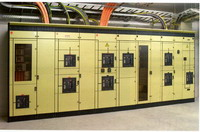
\includegraphics[scale = 0.8]{ReseauFlotsExempleArmoiresTableauxElectriques_okken_PCC.jpg}
%\caption{ \`A gauche :  Tableaux \'electriques entreprise Okken PCC, \`a Droite : baie de serveurs (\lhead{source: news.pixelistes.com}). }
%\label{exempleAmoiresTableauxElectriques}
%\end{figure}
\begin{table}[htb!] 
	\begin{tabular}{cc}
	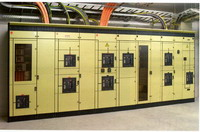
\includegraphics[scale = 1.20]{ReseauFlotsExempleArmoiresTableauxElectriques_okken_PCC.jpg} & 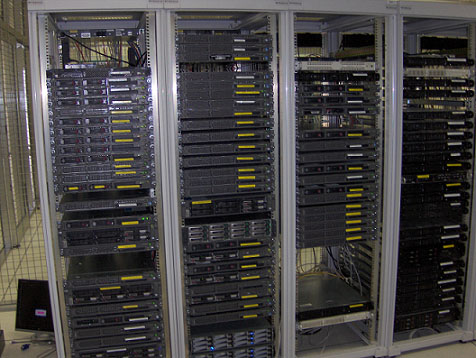
\includegraphics[scale = 0.5]{ReseauFlotsExemple_Baie_serveurs.jpg} \\
	\end{tabular}
	\caption{ Composants \'electriques d'un datacenter. \`A gauche :  tableaux \'electriques Okken PCC, \`a Droite : baie de serveurs (source: news.pixelistes.com). }
\label{exempleAmoiresTableauxElectriques}
%\vspace{-1.5cm}
\end{table}
%\FloatBarrier

% ---- figure exemple amoires et tableaux electriques



		\subsection{R\'eseau \'electrique : un graphe de flots}
			L'\'electricit\'e, achemin\'ee par le gestionnaire de r\'eseau, arrive aux transformateurs basse tension qui g\'en\'eralement fonctionnent en mode triphas\'e.
Ces transformateurs vont convertir la puissance {\em HTA} re\c cue ($20$KVA chez Enedis) en une puissance {\em BT} ($400$KVA) et cette puissance est envoy\'ee sur chaque phase.
Une phase est un canal de transport de courant et 
le courant d'une phase est exprim\'e en fonction du sinus et d'un d\'ecalage de $2\pi/3$ par rapport au courant d'une autre phase.
Chaque phase transporte cette \'energie aux divers tableaux. 
Chaque tableau peut \^etre rattach\'e \`a deux phases pour \'eviter les micro-coupures d'\'electricit\'e. Pendant ces micro-coupures, les accumulateurs et les groupes \'electrog\`enes prennent le relai dans le but d'\'eviter une interruption de service.
Les tableaux sont rattach\'es aux phases et aux baies par des c\^ables \'electriques. 
Chaque \'equipement mesure la quantit\'e d'\'electricit\'e qui le traverse.
Les c\^ables sont unidirectionnels. 
Aucun \'equipement ne s'alimente lui-m\^eme et les \'equipements de m\^eme nature ne sont pas rattach\'es entre eux. Par exemple, il n'existe aucun c\^able entre des tableaux et aucune baie n'alimente une autre baie.
L'\'electricit\'e suit un sens : des sources vers les baies. 
Chaque \'equipement mesure la quantit\'e d'\'electricit\'e qui le traverse. 
 Par convention, ces mesures sont port\'ees par les c\^ables incidents entrants dans chaque \'equipement.
\newline
Notre r\'eseau \'electrique se  mod\'elise avec un r\'eseau de flots dont le graphe est un graphe orient\'e sans circuit {\em Directed Acyclic Graph (DAG)} dans lequel
chaque sommet repr\'esente un \'equipement,
un arc repr\'esente des c\^ables \'electriques et 
 qu'aucun \'equipement ne s'alimente soi-m\^eme (absence de circuits dans le r\'eseau). 
		
{\bf Conclusion} : 
le r\'eseau \'electrique d'un data center comprend des sources, des tableaux, des baies de serveurs et  ils sont tous reli\'es  par des c\^ables \'electriques. Les \'equipements de ce r\'eseau ne s'alimentent pas soi-m\^eme et les \'equipements de m\^eme nature ne poss\`edent pas de c\^ables entre eux. Les c\^ables sont undirectionnels et l'\'electricit\'e a toujours le m\^eme sens : de la source aux baies.
Nous en concluons que la topologie du data center est un {\em graphe orient\'e sans circuit} induit par le sens de la circulation du courant \'electrique sur ces liens. Ainsi ce graphe est la topologie du r\'eseau \'electrique. 

		
% ----------------------------------------------------------------------------------------------------------------------------------
% 		Modelisation du graphe de flots electriques
% ----------------------------------------------------------------------------------------------------------------------------------
	\section{Mod\'elisation du r\'eseau \'electrique du data center}
		\subsection{Description du graphe de flots}
			
Soit $G=(V,A,CAP)$ le graphe orient\'e sans circuit mod\'elisant le r\'eseau \'electrique. 
Chaque sommet de $G$ est soit une source, soit  un tableau ou soit un serveur. 
L'ensemble des sommets $V$ est compos\'e des \'equipements sources $V_S$, interm\'ediaires ou passifs $V_I$ et  charges ou serveurs $V_C$. Il est une union disjointe, deux \`a deux, des partitions $V_C$, $V_I$ et $V_S$ de $V$ de cardinalit\'e $n$ dans laquelle :
\begin{itemize}
	\item Les sommets $V_S$ sont des sommets de degr\'e entrant nul $d^{-} = 0$.
	\item Les sommets $V_I$ sont des sommets de degr\'es entrant et sortant non nuls $d^{-} \ne 0, d^{+} \ne 0$.  
	\item Les sommets $V_C$ sont des sommets de degr\'e sortant nul  $d^{+} = 0$.
\end{itemize}
$$ 
V = V_S \cup V_I \cup V_C ~ et ~ 
V_S \cap V_I =  \emptyset ~ et ~ 
V_S \cap V_C =  \emptyset ~ et ~ 
V_C \cap V_I =  \emptyset
$$
L'ensemble des arcs $A$ mod\'elise $m$ c\^ables \'electriques.
Chaque arc a un flot, une capacit\'e et une r\'esistance consid\'er\'ee constante.
La capacit\'e de chaque arc est fonction de la grandeur associ\'ee \`a cet arc.
\newline
Par convention avec les \'equipes m\'etiers du r\'eseau, nous avons d\'ecid\'e que les arcs incidents entrants dans chaque sommet du graphe portent les mesures des grandeurs physiques.

		\subsection{Grandeurs, flots et contraintes physiques}
			Nous pr\'esentons les grandeurs physiques dans le r\'eseau \'electrique puis d\'efinissons la capacit\'e d'un arc et enfin d\'ecrivons les flots selon chaque grandeur pour un arc donn\'e.

			\subsubsection{Grandeurs physiques}
				Le r\'eseau \'electrique a deux modes de fonctionnement : le mode triphas\'e regroupant les grandeurs $U_{12}, U_{23}, U_{13}, I_{12}, I_{23}, I_{13}$ et le mode monophas\'e regroupant les grandeurs $I,U$. Les autres grandeurs sont communes aux deux syst\`emes (les grandeurs $P, Q, S, cos \phi$). Les symboles
  $U_{12}, U_{23}, U_{13}, U$ sont des tensions,
  $I_{12}, I_{23}, I_{13}, I$ des intensit\'es, 
  $P, Q, S$ des puissances actives, r\'eactives, apparentes respectivement et 
  $cos \phi$ ou $FP$ le facteur de puissance.
\newline 
Une grandeur physique sur un arc est une caract\'eristique physique mesurable selon une unit\'e de mesure. \\
Selon le ph\'enom\`ene physique pris en compte, les grandeurs physiques sont pr\'ed\'efinies. Dans le cas de l'\'electricit\'e, les grandeurs physiques forment l'ensemble \textbf{GP} de cardinalit\'e finie d\'efini comme suit :
\begin{equation}
	GP = \{I, I_{1}, I_{2}, I_{3}, U, U_{12}, U_{23}, U_{13}, P, Q, S, FP \}
\end{equation}
avec le facteur de puissance $FP$ qui d\'esigne le d\'ephasage entre l'intensit\'e ($I$) et la tension ($U$).
\newline
Ces deux modes (triphas\'e et monophas\'e) peuvent fonctionner dans le m\^eme r\'eseau. Cela implique qu'il n'existe qu'un seul sous-ensemble de grandeurs sur un arc, soit des grandeurs monophas\'ees soit des grandeurs triphas\'ees. On note $GP^{a_{i}}$ l'ensemble des grandeurs sur un arc $a_{i} $.
\begin{equation}
	\forall a_{i} \in A, \hspace{0.2cm}  GP^{a_{i}} \subset GP
\end{equation}
On distingue deux types de grandeurs :
\begin{itemize}
	\item Grandeurs \`a diff\'erentiel de potentiel : les tensions. On les note $gp_{ddp} \in \{U_{12}, U_{23}, U_{31}, U\}$.
	\item Grandeurs \`a effet calorique :  l'intensit\'e, la puissance active et r\'eactive. On les note $gp_{cal} \in \{ P, I_{1}, I_{2}, I_{3}, Q\}$.
\end{itemize} 
			\subsubsection{Capacit\'e d'un arc}
				Soit un arc $a_{i} \in A$ et $GP^{a_{i}} \in GP$ l'ensemble des grandeurs physiques associ\'ees \`a l'arc  $a_{i}$.
La  capacit\'e d'un arc $a_{i}$ est une fonction $Cap_{a_{i}}$ qui, pour chaque grandeur physique $GP^{a_{i}}$ associe une valeur r\'eelle positive $\R^{+}$.
\begin{equation}
	Cap_{a_{i}}: GP^{a_{i}} \rightarrow \R^{+}
\end{equation}
Le  vecteur $CAP$ contient les capacit\'es pour chaque grandeur et chaque arc.
\begin{equation}
	CAP = (Cap_{a}[x])_{ a \in A, x \in GP^{a} }
\end{equation}
			\subsubsection{ Description d'un flot physique}
				Les mesures physiques sont des valeurs de ces grandeurs.
%Le vecteur de mesures $gp(a, gp_{a})$ est de norme $T^{a,gp_{a}}$ associ\'e \`a l'arc $a$ et le i$^{ieme}$ \'el\'ement pris dans cette s\'erie de mesures est  $gp(a,gp_{a}, i)$. 
Le vecteur de mesures $gp_{a}^{x}$ de norme $T^{a,x}$ (c'est-\`a-dire le nombre de valeurs associ\'ees \`a une grandeur dans une s\'erie temporelle) est une s\'erie de mesures associ\'ee \`a l'arc $a$ et \`a la grandeur $x \in  GP^{a}$ dont le i$^{ieme}$ \'el\'ement est  $gp_{a}^{x}[i]$.
Le vecteur $gp_{a}^{x}$ associ\'e \`a la grandeur $x \in GP^{a}$ et \`a l'arc $a \in A$ est d\'efini comme suit :
\begin{equation}
	gp_{a}^{x} = ( gp_{a}^{x}[t] )_{0 < t < T^{a, x} }
\end{equation}
avec $ gp_{a}^{x}[t] \in \R^{+}$ et $ t \in \N^{+}$.
\begin{remark}
\label{remarque} 
Soient  $gp_{a}^{x}[t]$ le t$^{ieme}$ \'el\'ement de la s\'erie temporelle de la grandeur $x \in GP^{a}$ et $a, a'$ deux  arcs distincts.
\begin{itemize}
	\item  $gp_{a}^{x}[t]$ et  $gp_{a}^{y}[t]$, pour $x, y \in GP^{a}$ sont prises aux m\^emes instants.
	\item  pour $x\in GP^{a} \cap GP^{a'}$,  $gp_{a}^{x}[t]$ et  $gp_{a'}^{x}[t]$  sont prises \`a des instants diff\'erents.
\end{itemize}
\end{remark}
Certaines valeurs de $ gp_{a}^{x}$ sont ind\'efinies ou \'erron\'ees dans certains cas.

			\subsubsection{ Contraintes sur les flots}
				 \label{reglesLocales}
Un flot  $gp_{a}^{x}[t]$ est admissible s'il respecte, pour chaque arc $a \in A$ travers\'e, la contrainte ci-dessous:
\begin{equation}
	0 \le  gp_{a}^{x}[t] \le Cap_{a}[x]
\end{equation}	
avec $Cap_{a}$ la capacit\'e de l'arc $a$ pour la grandeur $x \in GP^{a}$.
\newline
Un flot est une fonction qui prend en entr\'ees 
un arc $a$, 
une grandeur $x \in GP^{a}$, 
un vecteur $gp_{a}^{x}$ associ\'e \`a la grandeur $x$ de l'arc $a$, 
un facteur de puissance $cos \phi$ ou $FP$ associ\'e  \`a l'arc $a$
et retourne un vecteur d\'efini comme suit :
\begin{equation}
	flo(a,x,gp_{a}^{x}) = f(a, x, r, cos \phi, gp_{a}^{x}) =
	\begin{cases}
		 \frac{  gp_{a}^{x} }{r \times cos \phi}, x \in gp_{ddp} \\
		 gp_{a}^{x} , x \in gp_{cal}
	\end{cases}
\end{equation}
avec $r$ la r\'esistance du c\^able, FP ou cos $\phi$ le facteur de puissance.
\newline
Une valeur $flo_{t}(a,x,gp_{a}^{x})$ de $flo(a,x,gp_{a}^{x})$ s'obtient \`a un indice $t < T^{a, x}$ donn\'e et se d\'efinit comme suit : 
\begin{equation}
	flo_t(a,x,gp_{a}^{x}) = f(a, x, r, cos \phi, gp_{a}^{x}) =
	\begin{cases}
		 \frac{  gp_{a}^{x}(t) }{r \times cos \phi}, x \in gp_{ddp} \\
		 gp_{a}^{x}(t) , x \in gp_{cal}
	\end{cases}
\end{equation}
Soient $a \in A$ un arc et $x \in GP^{a}$ une grandeur li\'ee \`a l'arc $a$.
L'ensemble des arcs incidents \`a $a$ ayant la m\^eme extr\'emit\'e initiale que $a$ est not\'e  $succ(a)$ et 
 l'ensemble des arcs incidents \`a $a$ ayant la m\^eme extr\'emit\'e finale que $a$ est not\'e $pred(a)$.
 Tous les \'el\'ements de $succ(a)$ et $pred(a)$ ont les m\^emes grandeurs physiques. 
 \newline
La fonction $flo$ doit respecter la contrainte de la loi de conservation $R$ \cite{loiDeConservation}. La loi de  conservation $R$ ne s'applique qu'avec les grandeurs \`a effet calorique $gp_{cal} \in GP$ et se d\'efinit  comme suit :
\begin{enumerate}
		\item 
			\begin{equation}
				\sum_{a_{j} \in pred(a)} flo_t(a_{j},x,gp_{a_{j}}^{x}) = \sum_{a_{k} \in succ(a)} flo_t(a_{k},x,gp_{a_{k}}^{x}) + \epsilon 
			\end{equation}
		avec $\epsilon$ les pertes par effets joules. Cette \'equation est la loi de conservation ou de Kirchhoff

%		\item L'extr\'emit\'e finale de $a$ est un puits ou noeud consommateur
%			\begin{equation}
%				si~ succ(a) = \emptyset ~ alors ~ \sum_{a_{j} \in pred(a)} flo_t(a,x,gp_{a}^{x}) \ge 0 
%			\end{equation}	
%		\item L'extr\'emit\'e initiale de $a$ est une source ou noeud source
%			\begin{equation}
%				si ~ pred(a) = \emptyset ~ alors ~ \sum_{a_{j} \in succ(a)} flo_t(a,x, gp_{a}^{x}) \ge 0 
%			\end{equation}	
\end{enumerate}


%Soient 2 arcs $a_{i}, a_{j}$ ayant une extr\'emit\'e en commun, et une grandeur physique $gp_{a} \in GP$.\\
%Un flot $flo$ est une fonction qui prend en entr\'ee un arc et une grandeur physique et qui fournit une valeur r\'eelle en sortie. 
%Le flot d\'epend des caract\'eristiques  de l'arc (r\'esistance, cos $\phi$) et se d\'efinit ainsi:
%\begin{equation}
%	flo(a,gp_{a}^{x}) = f(a, r, cos \phi, gp_{a}^{x}) =
%	\begin{cases}
%		 \frac{  gp_{a}^{x} }{r \times cos \phi}, x \in gp_{ddp} \\
%		 gp_{a}^{x} , x \in gp_{cal}
%	\end{cases}
%\end{equation}
%avec $x \in GP^{a}$, $r$ la r\'esistance du c\^able, FP ou cos $\phi$ le facteur de puissance. \\
%Le vecteur de flot $flo(a,gp_{a}^{x})$ est de norme $T^{a,x}$.\\
%Une valeur de $flo(a,gp_{a}^{x})$ s'obtient \`a un indice $t < T^{a, x}$ donn\'e c'est-\`a-dire $flo_{t}(a,gp_{a}^{x})$
%\begin{equation}
%	flo_{t}(a, gp_{a}^{x}) = f[a, r, cos \phi, gp_{a}^{x}, t] =
%	\begin{cases}
%		 \frac{  gp_{a}^{x}[t] }{r \times cos \phi}, gp \in \{U, U_{12}, U_{23}, U_{13}  \} \\
%		 gp_{a}^{x}[t] , gp \in \{P, Q, I, I_{1}, I_{2}, I_{3}  \}
%	\end{cases}
%\end{equation}
%La loi de conservation aussi nomm\'ee  \textbf{r\`egles locales $R$} ne s'applique qu'avec les grandeurs \`a effet calorique $gp_{cal} \in GP$ et se d\'efinisse  comme suit:
%	\begin{enumerate}
%		\item 
%			\begin{equation}
%				\forall a_{i} \in A_{gp},  \sum_{a_{j} \in P(a_{i})} flo(a_{j},gp_{a_{j}}^{x}) = \sum_{a_{k} \in S( a_{i} )} flo(a_{k},gp_{a_{k}}^{x}) + \epsilon 
%			\end{equation}
%		avec $\epsilon$ les pertes par effets joules. Cette \'equation est la loi de conservation ou de Kirchhoff
%
%		\item l'extr\'emit\'e finale de $a_{i}$ est un puits ou noeud consommateur
%			\begin{equation}
%				si \hspace{0,1cm} S( a_{i} ) = \emptyset \hspace{0,1 cm} alors \hspace{0,1cm} \forall a_{i} \in A_{gp}, \sum_{a_{j} \in S(a_{i})} flo(a_{j},gp_{a_{j}}^{x}) \ge 0 
%			\end{equation}	
%		\item l'extr\'emit\'e initiale de $a_{i}$ est une source ou noeud source
%			\begin{equation}
%				si \hspace{0,1cm} P( a_{i} ) = \emptyset \hspace{0,1cm} alors  \hspace{0,1cm} \sum_{a_{j} \in P(a_{i})} flo(a_{j}, gp_{a_{j}}^{x}) \ge 0 
%			\end{equation}	
%	\end{enumerate}
%avec $ S(a_{i}) = \{a_{j}: a_{i}^{-} = a_{j}^{-}   \}$ l'ensemble des arcs ayant la m\^eme extr\'emit\'e initiale que $a_{i}$ et 
% $ P(a_{i}) = \{a_{j}: a_{i}^{+} = a_{j}^{+}   \}$  l'ensemble des arcs ayant la m\^eme extr\'emit\'e  finale que $a_{i}$.
			\subsubsection{Description de Verif-correl}
				\label{VerifCorrel}
La fonction $Verif-correl$ d\'etermine le sous-ensemble d'arcs entrants et sortants d'un sommet du r\'eseau \'electrique en se basant sur les mesures physiques et les lois de conservation $R$ d\'efinies dans le paragraphe \ref{reglesLocales}. 
\newline
Soit $S \subset A$ l'ensemble  fini d'arcs incidents \`a un sommet  $v \in V$ et 
$x \in GP$ une grandeur physique 
telle que chaque arc $a \in S$ a un flot $gp_{a}^{x}$.
Nous partitionnons $S$ en deux sous-ensembles $S_1$ et $S_2$ tels que $S_1 \cap S_2  = \emptyset$.
\newline
La fonction $Verif-correl$ est bool\'eenne, prend en param\`etres $S_1$, $S_2$ et une grandeur $x$. 
Elle retourne $1$ si :
\begin{itemize}
	\item $S_1$ est l'ensemble des arcs entrants du sommet $v$.
	\item $S_2$ est l'ensemble des arcs sortants du sommet $v$.
\end{itemize} 
Si les lois $R$ ne sont pas v\'erifi\'ees alors $Verif-correl$ retourne $0$.
$$
Verif-correl(S_1, S_2, x) = 1 \Leftrightarrow  \sum_{ a_i \in S_1} gp_{a_i}^{x}(t) - \sum_{a_ j\in S_2} gp_{a_j}^{x}(t)  \le \epsilon 
$$
En effet, consid\'erons $t$ un instant de temps et 
		$diff(t) =  \sum_{ a_i \in S_1} gp_{a_i}^{x}(t) - \sum_{a_ j\in S_2} gp_{a_j}^{x}(t)$ 
la diff\'erence entre les flots entrants et sortants \`a un instant $t$.
La diff\'erence $diff(t)$ doit toujours \^etre inf\'erieure aux pertes par Effet Joule $\epsilon$ quel que soit l'instant $t$. 
\newline
Nous d\'ecidons que la fonction $Verif-Correl$ retourne $0$ si 
le nombre de diff\'erences $diff(t)$ sup\'erieure \`a $\epsilon$ est sup\'erieur \`a un seuil (choisi \`a $10\%$).
%la moyenne des diff\'erences $\frac{\sum_{t=0}^{T} diff(t)}{T}$  est sup\'erieure \`a un seuil (choisi \`a $10\%$).
\newline


Nous consid\'erons, dans la suite du rapport, que la {\em d\'ecision de $Verif-correl$ est toujours exacte}. Cela signifie que 
si $Verif-correl(S1, S2, x) = 0$ alors les arcs de $S$ ne partagent pas un sommet de $V$.
Cependant, dans la pratique, nous n'utilisons pas cette fonction pour d\'eterminer la topologie car pour un sommet $v$ de la topologie ayant un ensemble d'arcs $S_v$, nous devons  tester de l'ordre de $2^{|S_{v}|}$ bipartitions dans le pire des cas pour obtenir la bonne bipartition et cela est impossible pour $S_{v}$ tr\`es grand. 

%			 \subsubsection{ Influence des pertes par effets joules} 
%			 	%epsilon est le taux min des pertes par effets joules pour lequel l'oracle ne comet pas d'erreurs.
% EJ ce sont les pertes par effet joules dans le reseau.

% DECISION : ABANDON DE CE PARAGRAPHE car utilise les algorithmes de couvertures
Nous consid\'erons que le r\'eseau \'electrique modelis\'e par un DAG $G$ est connu.
Nous \'etudions l'\'evolution du pourcentage minimum des pertes par effets joules not\'ee $\epsilon$ en fonction des partitions coh\'erente propos\'ee par  {\em Verif-correl}.
Nous d\'efinissons la {\em similarit\'e} comme \'etant le pourcentage d'arcs de $A$ bien pr\'edits par $Verif-correl$.
Nous r\'ealisons deux exp\'eriences: 
\begin{itemize}
\item La premi\`ere exp\'erience consiste \`a g\'en\'erer des mesures de flots de divers graphes en faisant varier, de $0$ \`a $1$ par pas de $0.125$, les pertes par effets joules $EJ$ tout en fixant la variable $\epsilon$. Nous ex\'ecutons l'algorithme de couverture sur diff\'erents graphes, chaque graphe ayant un $EJ \in [0,1]$. Nous \'etudions l'\'evolution de la  similarit\'e en fonction de pertes joules $EJ$. 

\item La deuxi\`eme exp\'erience consiste \`a faire varier la variable $\epsilon$ en fixant la similarit\'e \`a $1$.  Nous \'etudions les variations des pertes en fonctions de $\epsilon$.  Les pertes par effets joules $EJ$ varient  de $0$ \`a $1$ par pas de $0.125$. 

\end{itemize}
Rappelons que $EJ=0.1$ signifie qu'il existe une diff\'erence de flot par grandeurs de $0.1$ entre les arcs ext\'erieures (sortantes) et int\'erieures (entrantes) \`a chaque sommet. Ainsi $EJ=0$ signifiant qu'il n'existe aucune perte tandis que  $EJ=1$ signifiant qu'il n'existe aucuns flots entre les arcs entrants et sortants d'un sommet du r\'eseau de flots.
% experience 1
\paragraph{exp\'erience 1} :
On fixe  $\epsilon=0.75$. 
La figure \ref{courbeEJCoef} resume les variations de {\em Verif-correl}. 
Le fait que la courbe de la variable $\epsilon$ est d\'ecroissante confirme notre hypoth\`ese selon laquelle il n'existe aucuns flots entre les arcs entrants et sortants d'un sommet lorsque les pertes par effets joules sont \'egales \`a $EJ = 1$. En effet, pour toute valeur de pertes par effets joules  $EJ=[0,0.3]$, le graphe propos\'e est identique au graphe du r\'eseau \'electrique. Par contre, {\em Verif-correl} se trompe deux sur trois sur les cliques fournies pour $EJ = ]0.3,0.9]$ parce que la coefficent de similarit\'e est de $0.38$. 
\begin{figure}
\centering
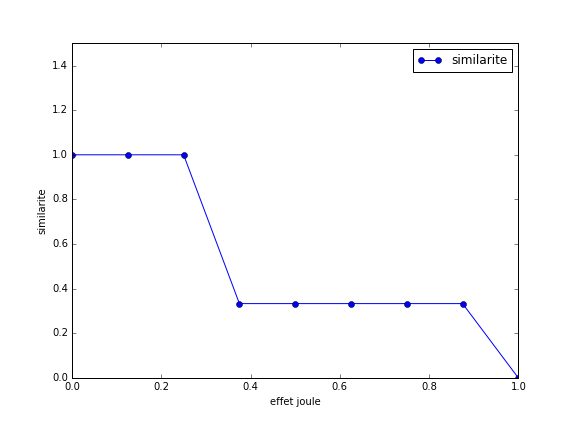
\includegraphics[scale=0.50]{courbe_similarite_selon_EJ_pour_epsilon_075.png}
\caption{ Le coefficient de similarit\'e en fonction des pertes par {\em effets joules} pour $epsilon=0.75$.}
\label {courbeEJCoef}
\end{figure}
\FloatBarrier

%experience 2
\paragraph{exp\'erience 2} :
Ici, on suppose la similarit\'e \'egale \`a $1$ et on cherche les variations de la variable $\epsilon$ en fonction des pertes par {\em effets joules}. 
Les pertes par {\em effets joules} varient de $[0,1]$ par pas de $0.125$ et nous distinguons $8$ intervalles [0,0.125], ]0.125,0.250], ]0.250,0.375], ]0.375,0.5], ]0.5,0.625], ]0.625, 0.75], ]0.75,0.875], ]0.875,1]. 
Pour chaque valeur $\epsilon$, on compte les intervalles $EJ_x, x \in [1,8]$ dans lesquelles la similarit\'e est \'egale \`a $1$ not\'e $X(\epsilon)$. Ainsi $X(\epsilon=0.3) = 8$ signifie que  les pertes par effets joules varient de $0$ \`a $1$ (EJ=[0,1]) et $X(\epsilon=0.3) = 2$ correspond \`a une variation de $EJ$ sur l'intervalle $[0,0.250]$.
On cr\'ee ainsi la distribution de $\epsilon$ en fonction des pertes par effets joules.
La figure \ref{courbeEpsilonEJ}  r\'esume cette distribution qui varie de $1$ (correspondant \`a une variation sur [0,0.125]) \`a $8$ (correspondant \`a une variation sur [0,1]).
La courbe de cette distribution est constante de l'intervalle $\epsilon = [0,0.125]$ puis  d\'ecroissante de l'intervalle $\epsilon =[0.125,1]$ et cette pente est tr\`es accentu\'ee dans l'intervalle $\epsilon = [0.8, 1]$. 
Au d\'el\`a  de $\epsilon > 0.8$, les pertes par effets joules varient dans l'intervalle $EJ=[0,0.2]$.
On en conclut que le meilleur intervalle est $\epsilon = [0.8, 1]$ pour produire des graphes de similarit\'e \'egale \`a $1$ en pr\'esence de pertes par {\em effets joules} de $20\%$.
\newline
% images
\begin{figure}
\centering
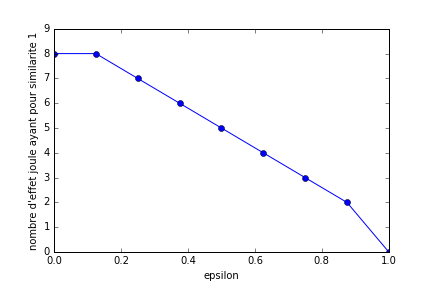
\includegraphics[scale=0.60]{courbe_epsilon_selon_nbreEJ_pour_similarite_1.png}
\caption{ Relation inverse entre $\epsilon$ et $EJ$: $8$ en ordonn\'e correspond \`a $[0,1]$, $7$ \`a $[0, 0.875]$ }
\label {courbeEpsilonEJ}
\end{figure}
\FloatBarrier

% conclusion
{\bf Conclusion} : Ces deux exp\'eriences montrent que la d\'ecision de la fonction {\em Verif-correl}  a une r\'elation inverse avec les pertes par effets joules ($EJ$). En effet, plus $\epsilon$ est petit plus les pertes par effets joules sont grandes et plus les d\'ecisions de {\em Verif-correl} sont erron\'ees.
\begin{equation}
	\epsilon > 1 - EJ
\end{equation}

		\newline 

{\bf Conclusion} :
le r\'eseau \'electrique est mod\'elis\'e par un graphe $G=(V,A,CAP)$.
L'ensemble des sommets $V$ est mod\'elis\'e par des \'equipements sources $V_S$, interm\'ediaires $V_I$ et serveurs $V_C$. Les sous-ensembles  $V_S, V_I, V_C$ sont disjoints deux \`a deux.
Chaque arc $a$ contient des grandeurs physiques $GP^{a}$. Nous en avons denombr\'e $8$ regroup\'ees en 
grandeurs \`a diff\'erentiel de potentiel $gp_{ddp} = \{U_{12}, U_{23},U_{31},U \}$ et en 
grandeurs \`a effet calorifique  $gp_{cal} = \{I_{1}, I_{2}, I_{3}, P \}$.
 Pour chaque grandeur physique $x \in GP^{a}$ associ\'ee \`a l'arc $a$, une capacit\'e $Cap_{a}$ et les mesures $gp_{a}^{x}$ lui sont associ\'ees.
Le flot de mesures $flo$ est un vecteur de mesures qui d\'epend de l'arc $a$, de la grandeur physique $x$ et de la mesure physique $gp_{a}^{x}$. Une valeur de flot $flo_t$  v\'erifie la loi de conservation $R$ et est d\'efinie comme suit :
\begin{equation}
	flo_{t}(a, x, gp_{a}^{x}) = f[a, x, r, cos \phi, gp_{a}^{x}, t] =
	\begin{cases}
		 \frac{  gp_{a}^{x}[t] }{r \times cos \phi}, gp \in \{U, U_{12}, U_{23}, U_{13}  \} \\
		 gp_{a}^{x}[t] , gp \in \{P, Q, I, I_{1}, I_{2}, I_{3}  \}
	\end{cases}
\end{equation}. 
\newline
Nous avons d\'efini la fonction $Verif-correl$, qui \'etant donn\'ee deux ensembles d'arcs $S_1$ et $S_2$, affirme si ces arcs concourent en un sommet $v \in V$ en attribuant  $S_1$ \`a l'ensemble d'arcs entrants et $S_2$ \`a l'ensemble d'arcs sortants du sommet $v$.
Nous consid\'erons que la reponse de $Verif-correl$ est toujours exacte.  
		
% ----------------------------------------------------------------------------------------------------------------------------------
%		 etat de l'art sur la reconstruction/decouverte de reseau
% ----------------------------------------------------------------------------------------------------------------------------------
	\section{\'Etat de l'art sur la d\'ecouverte de topologie}
		Notre probl\`eme de d\'ecouverte de topologie est d'identifier la topologie du r\'eseau \`a partir des mesures c'est-\`a-dire les extr\'emit\'es communes aux arcs dans le r\'eseau.
\newline
Il existe un grand int\'er\^et \`a la d\'ecouverte de topologie notamment dans les syst\`emes distribu\'es avec le d\'eploiement de nouvelles g\'en\'erations de capteurs qui permettent de collecter des mesures selon diff\'erentes granularit\'es (millisecondes, secondes, minutes, quart d'heure, etc).
La communaut\'e scientifique examine tr\`es peu comment interpr\'eter ces mesures et l'impact de celles-ci dans le r\'eseau.
En effet, beaucoup de travaux sont orient\'es sur la d\'ecouverte de la topologie au moyen de protocoles r\'eseau. Des sondes sont propag\'ees dans le r\'eseau omettant la pr\'esence de capteurs dans les r\'eseaux. D'autres travaux cherchent \`a pr\'edire la topologie du r\'eseau informatique \`a partir des lois statistiques et des mod\`eles de files d'attentes.
\newline
Nous regroupons ces travaux en troix axes.
Les deux premiers axes font principalement de la m\'etrologie et cela leur permet de d\'eduire la topologie en connaissant les caract\'eristiques de chaque lien et de chaque n\oe ud du syst\`eme.
Le dernier axe porte sur la reconstruction de la topologie par les s\'eries temporelles.

\subsection{D\'ecouverte des topologies par des sondes}
La d\'ecouverte de topologie est un sujet important dans les r\'eseaux informatiques.
En effet, dans ces r\'eseaux,  on connait la topologie physique et les n\oe uds mais on ignore l'\'etat des n\oe uds. On recherche alors la topologie fonctionnelle du r\'eseau (l'interconnexion entre les n\oe uds) selon l'\'etat des n\oe uds. 
Il existe de nombreux outils pour sonder et faciliter les t\^aches d'administration de ces r\'eseaux. 
Ces outils permettent aux administrateurs r\'eseau de manager efficacement et de d\'ecouvrir le r\'eseau.
Nous citons HP OpenView \cite{OpenView} capable de localiser une erreur et d'envoyer des notifications de plusieurs \'ev\`enements. Ces \'ev\`enements incluent principalement des pertes dans le r\'eseau et les informations sur les caract\'eristiques des liens.
L'inconv\'enient de ces outils est leur co\^ut et ils ne sont pas abordables pour les petites et moyennes organisations.
La d\'ecouverte de r\'eseaux informatiques s'effectue  aussi avec des protocoles r\'eseaux dont les plus connus sont ICMP \cite{rfc792} et SNMP \cite{rfc2821}.
Divers algorithmes ont \'et\'e propos\'es. 
Nous pouvons citer l'algorithme de {\em Narayan et al.} \cite{Breitbart:2004:TDH:1008463.1008464} qui r\'ealise la d\'ecouverte de topologie et de services pour des r\'eseaux h\'et\'erog\`enes en se servant du syst\`eme netInventory \cite{breitbart2004topology}. 
Cet algorithme est bas\'e sur deux hypoth\`eses : 
$(i)$ chaque domaine doit avoir un seul sous-r\'eseau et 
$(2i)$ les tables de routage sont compl\`etes. 
Pour la d\'ecouverte de topologie, le syst\`eme {\em netInventory} \'enum\`ere la liste des adresse IP, envoie des messages ECHO ou ICMP pour d\'eterminer si un n\oe ud est actif. Dans le cas o\`u PING est d\'esactiv\'e, netInventory se sert de ipRouteTable et ipNetToMediaTable dans les routeurs pour connaitre l'\'etat d'un n\oe ud.
\newline
De m\^eme, l'algorithme propos\'e par {\em Kuangyu Qin} \cite{QinKuangyuChunquan2010} est bas\'e sur {\em SNMP} et suppose que l'administrateur r\'eseau est connect\'e \`a l'interface de routage et envoie des paquets de d\'ecouverte aux routeurs. La station de gestion d\'ebute la d\'ecouverte par la lecture des tables de routage. En utilisant les MIB (Management Information Base) et les agents SNMP, cet algorithme \'elimine les \'equipements redondants et g\'en\`ere une topologie efficiente m\^eme quand il existe des VLAN dans le r\'eseau.
\newline
Un autre algorithme, propos\'e par {\em Bilal Saeed, TarekSheltami et Elhadi Shakshuki} \cite{SAEED2015104}, est bas\'e sur netInventory et acc\'el\`ere la d\'ecouverte de la topologie sans g\'en\'erer un trafic suppl\'ementaire. Cet algorithme, nomme TDA (Topology Discovery Algorithm), se sert de la programmation parall\`ele pour g\'erer toutes les requ\^etes de d\'ecouverte des interconnexions r\'eseaux sur la plateforme Android.
Une \'etude bibliographique, effectu\'ee par {\em Ahmed et al.} \cite{AhmedRafatAbouchabaka2014}, fournit les diff\'erentes techniques et algorithmes pour la d\'ecouverte de topologie de r\'eseaux informatiques. Les auteurs d\'eclarent que la plupart des algorithmes de d\'ecouverte de topologie physique de r\'eseau sont bas\'es sur le protocole SNMP. En d'autres termes, ils supposent que tous les n\oe uds de ce r\'eseau sont repertori\'es et activ\'es au moment de la d\'ecouverte. 
\newline

{\bf Conclusion} :
cette m\'ethode est contraire \`a notre sujet de recherche dans lequel nous ignorions les n\oe uds de notre r\'eseau.

\subsection{Tomographie des r\'eseaux}
La tomographie de r\'eseaux est une m\'ethode qui \'etudie les caract\'eristiques internes d'un r\'eseau (c'est-\`a-dire les liens et n\oe uds ON/OFF, la bande passante, la congestion du r\'eseau) en utilisant les mesures point-\`a-point (entre n\oe uds) obtenues \`a partir des sondes plac\'ees dans ce r\'eseau et en supposant que le r\'eseau est mod\'elisable (on peut d\'efinir un mod\`ele avec l'estimateur du maximum de vraisemblance ou l'inf\'erence bay\'esienne). Il fait aussi la pr\'ediction de la topologie du r\'eseau.
\newline
Cette m\'ethode est utilis\'ee en l'absence de syst\`eme de supervision fiable pour identifier les caract\'eristiques des liens et faire un diagnostic de ce dernier (quel n\oe ud/lien est indisponible, congestionn\'e ou ajout\'e) car il est impossible de contr\^oler les flux et l'\'etat des \'equipements.
Les probl\`emes, r\'esolus par la tomographie des r\'eseaux,  sont regroup\'es en $3$ cat\'egories :

\subsubsection{L'estimation des param\`etres (caract\'eristiques) d'un lien}

L'article de {\em Ghita et al.} \cite{ghitaArgyrakiThiran2010} se propose de d\'ecouvrir la congestion des liens dits "corr\'el\'es" dans un r\'eseau informatique.
Un lien entre deux n\oe uds du r\'eseau est une connexion logique au niveau de la couche $3$ du protocole TCP/IP et deux liens sont corr\'el\'es s'ils appartiennent au m\^eme domaine ou sous-r\'eseau.
Pour r\'ealiser cet algorithme, il consid\`ere que la topologie du r\'eseau et le degr\'e de corr\'elation entre les liens sont connus et qu'il existe un trafic unicast entre les n\oe uds dans le r\'eseau (ce trafic est d\'esign\'e par chemin).
Il \'enonce quatre hypoth\`eses pour l'exp\'erimentation de l'algorithme : 
$(i)$ l'ensemble des chemins reste inchang\'e durant chaque simulation; 
$(2i)$ chaque chemin est congestionn\'e si au moins un lien du chemin est congestionn\'e; 
$(3i)$ le comportement de congestion de chaque lien pendant chaque simulation est mod\'elis\'e par un processus al\'eatoire stationnaire; 
$(4i)$ deux ensembles de corr\'elations disjoints ne doivent pas \^etre travers\'es par les m\^emes chemins.
\newline
Diff\'erentes m\'ethodes ont \'et\'e propos\'ees et valid\'ees mais elles diff\`erent de l'algorithme {\em Ghita et al.} \cite{ghitaArgyrakiThiran2010} par les caract\'eristiques des liens fournis.
En effet, les m\'ethodes initiales se basent sur les corr\'elations temporelles, chacune parfaitement corr\'el\'ee et envoy\'ee par des packets multicast \cite{adamsBuFreidmanHorowitz2000, aryaDuffieldVeitch2008, buDuffieldPrestiTowsley2002, caceresDuffieldHorowistzTowsley1999}. 
Tous les taux de pertes des liens sont statistiquement identifiables dans une topologie en arbre \cite{chenCaoBu2007}.
Cependant le multicast n'est pas largement d\'eploy\'e et les groupes de paquets unicast exigent un d\'eveloppement subtantiel et un co\^ut d'administration \'elev\'e. D'o\`u il est moins ais\'e de s\'electionner les corr\'elations temporelles.
\newline
L'ensemble des m\'ethodes qui suivent \cite{nGDuffield2006, padmanabhanQiuWang2003,sommerBarfordDuffieldRon2007, zhaoChenBindel2006} utilisent seulement des mesures unicast point-\`a-point (c'est-\`a-dire des mesures sur les liens) dans le simple but d'identifier les congestions de liens.
\newline
Les m\'ethodes bool\'eennes de tomographie de r\'eseaux consid\`erent des hypoth\`eses suppl\'ementaires \cite{padmanabhanQiuWang2003,nGDuffield2006} pour identifier les liens congestionn\'es en trouvant le plus petit ensemble de liens qui peut \^etre expliqu\'e par ces mesures.
Ces hypoth\`eses sont : 
$(i)$ les liens sont ind\'ependants;
$(2i)$ les liens sont congestionn\'es \'equiprobablement; 
$(3i)$ le nombre de liens congestionn\'es est faible.
Toutes les pr\'ec\'edentes m\'ethodes \cite{ghitaArgyrakiThiran2010, nGDuffield2006, padmanabhanQiuWang2003,sommerBarfordDuffieldRon2007, zhaoChenBindel2006} se basent sur l'ind\'ependance des liens c'est-\`a-dire l'hypoth\`ese $(i)$.

\vspace{-0.4cm}  
\subsubsection{La pr\'ediction de topologie} 

L'objectif de cette m\'ethode est d'identifier l'arbre de la topologie connectant un serveur aux autres machines du r\'eseau.
L'id\'ee est d'utiliser une fonction croissante (ou monotone) du nombre de liens partag\'es entre deux n\oe uds ou le maximum de vraisemblance pour trouver l'arbre.
\newline
L'article de {\em Coates and al.} \cite{coatesCastroNowak2002} suppose que les mesures de la couche $2$ (protocole TCP/IP) des machines clientes sont assez fiables pour d\'ecouvrir le r\'eseau. Les mesures sont collect\'ees \`a l'aide de l'outil Traceroute. Ensuite l'auteur d\'efinit un mod\`ele bas\'e sur les chaines de Markov de Monte Carlo pour d\'eterminer les caract\'eristiques des liens du r\'eseau et d\'eduire les topologies probables. Enfin il propose un crit\`ere global du seuil maximum pour l'identification de topologie contrairement aux autres travaux \cite{andrieuDoucetFitzgerald2000bayesian, bestavrosAzerByers2005inference} qui emploient des strat\'egies semi-optimales de fusion des liens.
 
\subsubsection{La densit\'e du trafic entre \'emetteur/recepteur}

 Un probl\`eme de tomographie de r\'eseaux qui retient notre attention est l'estimation de la matrice de trafic qui pr\'evoit le volume de flots entre les n\oe uds point-\`a-point \`a partir des mesures \cite{vardi1996, caoDavisWielYu2000}.
En effet, les variables inconnues sont les volumes de flots et nous suivons une certaine loi de probabilit\'e.
\newline
Les corr\'elations de flots ont \'et\'e \'etudi\'ees par {\em Singal et Michailidis} \cite{singalMichailidis2007} et ils montrent que, sous certaines classes de d\'ependances, les moments d'ordre $n$ de ces volumes de flots sont identifiables \`a partir des mesures de liens pour $n \ge 2$.
Cette approche diff\`ere de $2$ aspects par rapport \`a l'estimation des caract\'eristiques de liens.
Premi\`erement, l'estimation des caract\'eristiques s'int\'eresse aux mesures point-\`a-point c'est-\`a-dire sur les liens tandis que le calcul du trafic point-\`a-point doit \^etre estim\'e dans la densit\'e de trafic \cite{vardi1996, singalMichailidis2007, caoDavisWielYu2000}.
Deuxi\`emement, l'estimation des caract\'eristiques utilise les variables bool\'eennes et la connaissance des valeurs des variables des lois de distributions n'est pas n\'ecessaire comme cela se fait dans la densit\'e de trafic. La connaissance des valeurs des param\`etres engendre la restriction de l'extension des r\'esultats th\'eoriques \cite{singalMichailidis2007}.
\newline

{\bf Conclusion} :
la tomographie de r\'eseaux n'est pas appropri\'ee pour notre sujet de recherche car nos mesures d'arcs d\'eterminent les caract\'eristiques de ces arcs et les n\oe uds sont inconnus emp\^echant la d\'ecouverte de r\'eseau qui est l'\'etape n\'ecessaire pour d\'ebuter la tomographie de r\'eseaux.


\subsection{Reconstruction de la topologie par les s\'eries temporelles}
Le brevet de {\em Chaudhary et al.} \cite{chaudhary2016network} d\'ecrit comment trouver le graphe induit par un r\'eseau de canalisations de fluides en se servant des mesures de capteurs de diff\'erentes stations qui \'emettent des fluides. Il consid\`ere le r\'eseau comme un arbre dans lequel la racine est une station comprenant un compresseur. La pr\'esence du compresseur induit un d\'elai de livraison entre la station source et les stations de livraison (d\'elai d'acheminement du fluide entre les n\oe uds du r\'eseau). 
Le d\'elai est d\^u au temps mis par le fluide pour atteindre la station de livraison. 
\newline
Le traitement des mesures \cite{cincotta1995astronomical, hurley2011methods, mohanty2000robust} porte sur la recherche de pics, la suppression d'anomalies (observations non conformes \`a un motif dans le dataset de donn\'ees) et le lissage des donn\'ees. 
Les donn\'ees obtenues identifient la relation d'adjacences entre les n\oe uds.
Le traitement des retards temporels d\'eterminent la distance entre des n\oe uds du r\'eseau.
L'analyse des s\'eries temporelles par paires d\'etermine la causalit\'e entre les capteurs associ\'es. 
La causalit\'e est la recherche d'\'ev\`enements identiques observ\'es dans deux s\'eries de mesures.
En d'autres termes, la causalit\'e consiste \`a savoir si les \'ev\`enements, observ\'es dans une s\'erie de mesures, se reproduisent dans une autre s\'erie. 
Un mod\`ele de causalit\'e bas\'e sur les s\'eries temporelles des stations est d\'efini comme une r\'egression multiple avec un mod\`ele de Granger.
\`A partir de ce mod\`ele, on calcule les diff\'erents retards $X(t)$ et leurs coefficients.
On d\'efinit \'egalement un mod\`ele de p\'enalisation bas\'e sur une r\'egression LASSO afin de filtrer les relations de causalit\'e et obtenir un graphe creux (sparse). 
Le graphe de causalit\'e est alors un arbre.
\newline
Les auteurs {\em Chaudhary et al.}  proposent un script s'ex\'ecutant r\'ecursivement sur les n\oe uds du r\'eseau en choisissant, \`a chaque \'etape, les n\oe uds qui ne sont pas des puits. En se servant du graphe de causalit\'e (corr\'elation) et des retards de propagation, il d\'etermine les voisins du n\oe ud $X_i$ et supprime les n\oe uds voisins de $X_i$  ayant une causalit\'e entre eux car le r\'eseau est un arbre.
\newline
La m\'ethode d\'ecrite ici est la construction du graphe it\'erativement \`a partir des sous-arbres du graphe. 
En effet, le nombre de sous-arbres est l'ordre dans lequel on a supprim\'e les n\oe uds puits. 
Cette m\'ethode est r\'ealisable en $O(n^2)$ car chaque sommet est trait\'e une fois et la recherche de son voisinage est en $O(n)$ avec $n$ le nombre de sommets.
\newline 
Cette m\'ethode est inadapt\'ee pour un DAG car sa complexit\'e est en $O(n^n)$.
Elle ne s'ex\'ecute que sur des arbres.
\newline
		\newline
{\bf Conclusion} :
l'\'etude bibliographique effectu\'ee sur la d\'ecouverte de topologie montre que la recherche sur ce sujet  est tr\`es active dans le domaine des r\'eseaux informatiques, pr\'ecisement dans la d\'etection de n\oe uds/liens congestionn\'es. 
Toutefois, dans le domaine \'energ\'etique, les rares travaux r\'ealis\'es sur ce sujet mettent l'accent sur la d\'ecouverte de topologie par la reconstruction des sous-graphes en supposant que les n\oe uds du r\'eseau sont connus, 
que certains liens sont absents, 
que les mesures sont influenc\'ees par les incidents 
et que des erreurs peuvent \^etre pr\'esentes sur nos donn\'ees. 
Ces travaux s'av\`erent moins pertinents pour notre probl\'ematique parce  que les r\'esolutions propos\'ees s'appuyent sur des hypoth\`eses qui sont diff\'erentes des n\^otres. 
En effet, nous connaissons que les liens et les mesures qui circulent sur ces liens. 
Mais nous ignorons exactement les extr\'emit\'es de ces liens.
Par ailleurs, ces mesures suivent  des lois physiques qui impliquent la propagation d'\'ev\`enements dans ces r\'eseaux.
Notre probl\'ematique est alors de d\'eterminer les extr\'emit\'es partag\'ees entre les liens  gr\^ace aux lois et aux mesures physiques et aussi \`a la th\'eorie des graphes.


	

% ----------------------------------------------------------------------------------------------------------------------------------
%		problematique
% ----------------------------------------------------------------------------------------------------------------------------------
	\section{Probl\`eme de d\'ecouverte de topologie \'electrique}
		Notre probl\`eme est de d\'ecouvrir la topologie d'un r\'eseau \'electrique dont on ignore les sommets et on ne connait que les flots dans chaque arc.
% --------- modelisation probleme ===> Donnees
%\subsection{Donn\'ees}
\begin{enumerate}
\item {\bf Donn\'ees} : 
\newline
Nous  avons donc
\begin{itemize}
	\item Un ensemble d'arcs distincts $2$ \`a $2$ du graphe $G$ dont les extr\'emit\'es \textbf{initiales} et \textbf{finales} sont inconnues.\\ $ A =\{ a_{1}, ... , a_{m} \} $ 
		
	\item \`A chaque arc sont associ\'ees des s\'eries de mesures $M(a_{i})$. \\
		$\forall a \in A$, $M(a) = ( gp_{a}^{x})_{x\in GP^{a}}$
		
	\item Chaque s\'erie de mesures $ gp_{a}^{x}$ est de norme $T^{a, x}$ v\'erifiant la remarque de la section ~\ref{remarque},  $x \in GP^{a} \subset GP$
	
	\item $\forall t < T^{a, x}$, $  gp_{a}^{x}[t] $ respecte les r\`egles dans $R$.
\end{itemize}
% --------- modelisation probleme ===> objectif
%\subsection{Objectif}
\item {\bf Objectif} : 
\newline
D\'eterminer la topologie  du graphe $G$ \`a partir des flots des arcs $M(a_{i})$ et des r\`egles $R$ c'est-\`a-dire $\forall a_i$, d\'eterminer $n_1,n_2$ tels que $a_i = (n_1,n_2)$.

% --------- approche
%\subsection{Approche}
\item {\bf Approche} :
\newline
Notre objectif est de d\'eduire la topologie du r\'eseau \'electrique repr\'esent\'ee sous la forme d'un graphe de flots. Notre approche se subdivise en deux \'etapes :
\begin{enumerate}
	\item La premi\`ere \'etape consiste \`a la recherche d'arcs ayant des extr\'emit\'es communes. Pour ce faire, nous calculons la similarit\'e entre les paires de mesures d'arcs pour chaque grandeur dans le but  de d\'eterminer les arcs corr\'el\'es puis nous construirons la matrice de corr\'elation. 
	\item La seconde \'etape est la construction du graphe \`a partir de la matrice de corr\'elation. 
\end{enumerate}


\end{enumerate}
			
% ----------------------------------------------------------------------------------------------------------------------------------
%		 conclusion
% ----------------------------------------------------------------------------------------------------------------------------------
	\section{Conclusion du chapitre \ref{ReseauFlotsMesures}}
		Dans ce chapitre, nous avons montr\'e que 
le r\'eseau \'electrique se mod\'elise par un graphe de flots dont les sommets sont des \'equipements, les arcs sont les c\^ables \'electriques unidirectionnels et les flots par les mesures des \'equipements. Par convention, ces mesures sont port\'ees par les arcs incidents entrants dans chaque sommet du graphe. 
Chaque mesure est associ\'ee \`a une grandeur physique et \`a chaque grandeur est d\'efinie une capacit\'e sur l'arc. Nous avons red\'efini la loi de conservation $R$ en fonction de nos mesures,  de nos grandeurs et nos capacit\'es.  
\newline
%Dans ce graphe, les arcs et leurs flots sont connues mais les sommets sont inconnues. Notre probl\`eme est de d\'eterminer les sommets communs aux arcs.
Dans ce graphe, nous connaissons les liens et les mesures qui circulent sur ces liens. 
Mais nous ignorons exactement les extr\'emit\'es de ces liens.
Par ailleurs, ces mesures suivent  des lois physiques qui impliquent la propagation d'\'ev\`enements dans ces r\'eseaux.
Notre probl\`eme est alors de d\'eterminer les extr\'emit\'es partag\'ees entre les liens  gr\^ace aux lois $R$, aux mesures physiques et aussi \`a la th\'eorie des graphes.
\newline
Une \'etude bibliographique a \'et\'e r\'ealis\'ee sur la d\'ecouverte de topologie. Les travaux concernent principalement la reconstruction de topologie dans le domaine informatique \`a partir de sondes et de protocoles de r\'eseau. Ces travaux s'accentuent sur la supervision de r\'eseau, l'administration du r\'eseau et aussi sur la recherche des caract\'eristiques des \'el\'ements du r\'eseau. 
Dans le domaine \'energ\'etique, nous avons trouv\'e un brevet qui reconstruit des sous-graphes du r\'eseau \`a partir de la propagation des incidents.
Tous ces travaux supposent que nous connaissons l'\'etat de tous les \'el\'ements du r\'eseau. Ce qui est contraire \`a notre probl\'ematique.
\newline
 Nous avons propos\'e deux approches pour r\'esoudre notre probl\`eme. La premi\`ere approche consiste \`a d\'eterminer la corr\'elation entre les arcs \`a partir des mesures et des r\`egles de flots puis \`a construire une matrice de corr\'elation. La seconde approche d\'ecouvre le r\'eseau en effectuant certaines transformations sur la matrice de corr\'elation.  

		
	
	%---- chapitre 2 : timeSeries et similarite entre series
	

\chapter{Mesures : Des S\'eries Temporelles}
\label{timeSeries}
Les mesures sur les arcs forment des s\'eries temporelles.
Certains arcs partagent des \'equipements que nous souhaitons d\'eterminer \`a partir des s\'eries temporelles. Nous supposons que les  s\'eries temporelles associ\'ees \`a ces arcs ont les m\^emes comportements au cours du temps. En d'autres termes, toute variation dans une s\'erie est visible dans une autre s\'erie. Nous disons que ces arcs sont {\em corr\'el\'es} et la valeur li\'ee \`a cette relation entre les arcs est d\'esign\'ee par {\em coefficient de similarit\'e}.  
\newline
Dans le chapitre pr\'ec\'edent, 
nous avons mod\'elis\'e les mesures sur les arcs par des s\'eries temporelles et la particularit\'e de ces s\'eries  est la pr\'esence de valeurs \'erron\'ees et manquantes. 
% quel est notre probleme
\newline
Le probl\`eme est de savoir s'il existe une m\'ethode de calcul du coefficient de similarit\'e qui tienne compte des erreurs dans les s\'eries temporelles et qui v\'erifie l'hypoth\`ese sous-jacente.
\newline
Pour ce faire, nous proc\'edons comme suit : la premi\`ere partie \'enonce  les analyses sur les s\'eries temporelles. La seconde partie pr\'esente les diff\'erentes m\'ethodes de calcul des coefficients de similarit\'e entre les s\'eries. Et enfin la derni\`ere partie s\'electionne la m\'ethode de calcul du {\em coefficient de similarit\'e} puis analyse les performances de cette m\'ethode sur les donn\'ees r\'eelles d'un {\em sous-r\'eseau du datacenter Champlan}.  

\section{S\'eries temporelles}
\begin{definition}
Une s\'erie temporelle est une suite chronologique de valeurs r\'eelles $x_t$ \`a des instants de temps r\'eguli\`erement espac\'es. 
% formule
\begin{equation}
(x_t)_{ t \in \Theta}
\end{equation}
avec $\Theta $ l'ensemble discret et fini des espaces de temps de dimension $n$.
\end{definition}
L'intervalle de temps entre deux mesures successives d\'epend de la s\'erie. 
Il peut s'agir d'une minute, d'une semaine, d'un jour, etc.
%G\'en\'eralement, les s\'eries temporelles s'utilisent dans les probl\`emes suivants :
G\'en\'eralement, les s\'eries temporelles sont utilis\'ees  pour comprendre les m\'ecanismes qui produisent ces observations. Ces m\'ecanismes sont associ\'es au temps et  permettent de faire les analyses suivantes :
\begin{itemize}
	\item La mod\'elisation : la repr\'esentation de la s\'erie sous la forme d'une fonction du temps.
	\item La pr\'evision : pr\'edire les donn\'ees futures \`a partir de valeurs pr\'ed\'ecentes.
	\item La d\'etection de rupture :  la s\'erie change-t-elle significativement \`a un instant $t$.
	\item La comparaison :  d\'eterminer la relation existante entre une s\'erie observ\'ee et d'autres s\'eries candidates.
\end{itemize}
Nous d\'ecrivons bri\`evement les mod\`eles d'analyses sur des s\'eries temporelles puis nous pr\'esentons l'objectif recherch\'e par l'analyse de ces s\'eries dans notre \'etude. 

\subsection{La mod\'elisation et la pr\'evison d'une s\'erie temporelle}
Un mod\`ele est une image simplifi\'ee de la r\'ealit\'e qui vise \`a traduire le fonctionnement d'un ph\'enom\`ene et permet de mieux les comprendre.
Nous distinguons deux types de mod\`eles :
\begin{itemize}
	\item Les mod\`eles d\'eterministes : ils utilisent les \'el\'ements de la statistique descriptive et suppose que l'observation de la s\'erie \`a la date $t$ est une fonction du temps $t$ et d'une variable $\epsilon_t$: 
	$$x_t = f(t, \epsilon_{t}).$$ 
	La variable $\epsilon_t$ est le r\'esidu ou l'erreur du mod\`ele et elle repr\'esente la diff\'erence entre la r\'ealit\'e et le mod\`ele propos\'e. 
	\newline
	Les deux mod\`eles les plus utilis\'es sont les suivants :
	\begin{itemize}
		\item Le mod\`ele additif : c'est la d\'ecomposition de la s\'erie en trois termes
			$$x_t = Z_t + S_t + Q_t $$ o\`u $Z_t$ est la tendance, $S_t$ la p\'eriodicit\'e et $Q_t$ les composantes (erreurs) identiquement distribu\'ees. $Z_t$, $S_t$ sont aussi d\'eterministes.
		\item Le mod\`ele multiplicatif : la variable $x_t$  est le produit de la tendance et d'une composante p\'eriodique :
		$$x_t = Z_t(1 + S_t)(1 + Q_t).$$
		Toutefois, l'application d'un logarithme nous permet de revenir au mod\`ele additif.
		$$y(t) = log(x_t) = log(Z_t) +log(1 + S_t) + log(1 + Q_t).$$
	\end{itemize}
	%L'utilisation de mod\`eles d\'eterministes pour la pr\'evision est \'el\'ementaire. Une fois d\'etermin\'ee la fonction $f$ \`a partir des donn\'ees observ\'ees $x_1 , ... , x_n$ , nous proposons une pr\'evision \`a la prochaine date par $\hat{X_{n+1}} = f(n+1)$.La pr\'ecision de cette pr\'evision peut aussi \^etre \'evalu\'ee par une estimation de la variance de $\epsilon_{n+1} = \hat{X_{n+1}} - f(n+1)$ . Cette estimation est r\'ealis\'ee par la variance empirique de la s\'erie des \'ecarts $\epsilon_i = X_{i} - f(i)$, consid\`er\'ee comme une s\'erie de variables al\'eatoires ind\'ependantes de m\^eme loi. La donn\'ee de cette variance empirique permettra de proposer un intervalle de confiance autour de la pr\'evision.

	\item Les mod\`eles stochastiques : ils font l'hypoth\`ese que les r\'esidus $\epsilon_t$ ne sont pas ind\'ependants et qu'il est possible de pr\'evoir les r\'esidus en partie. L'avantage r\'eside dans la r\'eduction de l'impr\'ecision de la pr\'evision des termes futurs de la s\'erie temporelle.  La variable $\epsilon_t$ devient une fonction des valeurs du pass\'e et d'un terme d'erreur $\eta_t$ $$\epsilon_t = (\epsilon_{t-1}, \epsilon_{t-2}, ... , \eta_{t}).$$
	Nous pouvons citer, comme exemple de mod\`eles couramment utilis\'es, les mod\`eles SARIMA, ARIMA et ARMA. Dans ces mod\`eles, la mod\'elisation porte sur la forme du processus $(\epsilon_t)$. Un exemple de mod\'elisation est le mod\`ele autor\'egressif lin\'eaire d'ordre $2$ avec des coefficients autor\'egressifs $a_1$, $a_2$ d\'efinis par 
	$$\epsilon_t = a_1 x_{t-1} + a_2 x_{t-2} + \eta_t,$$ o\`u $\eta_t$ est un bruit blanc.
\end{itemize}
Un exemple de s\'erie temporelle et de ses diff\'erentes composantes est pr\'esent\'e dans la figure \ref{exempleSerieTemporelleComposante}. La s\'erie temporelle est la donn\'ee du trafic prise chaque mois des routes fran\c caises de $1989$ \`a $1996$.
La premi\`ere ligne est la r\'epresentation de la s\'erie temporelle et la seconde est celle de la tendance. Quant \`a la troisi\`eme  et la derni\`ere ligne, elles repr\'esentent respectivement la figure de p\'eriodicit\'e et les r\'esidus. La p\'eriode de la s\'erie est de $12$.
% ---- figure exemple de la serie temporelle et ses composante
\begin{figure}[htb!] 
\centering
\includegraphics[scale = 0.5]{exempleSerieTemporelleComposante.pdf}
%\includegraphics[scale = 0.5]{/home/willy/Downloads/exempleSerieTemporelleComposante.pdf}
\caption{ 
	D\'ecomposition de la s\'erie temporelle representant les valeurs mensuelles du trafic routier de l'autoroute $A7$ de $09/1989$ \`a $09/1996$. Repr\'esentation des composantes de la s\'erie temporelle.} 
\label{exempleSerieTemporelleComposante}
\end{figure}
%\FloatBarrier
% ---- figure exemple de la serie temporelle et ses composante

Les deux types de mod\`eles ci-dessus induisent des techniques de pr\'evision bien particuli\`eres. 
Sch\'ema--tiquement, ils s\'eparent la tendance de la saisonnalit\'e \'eventuelle. Puis ils cherchent \`a les mod\'eliser et \`a les estimer.  Enfin ils les \'eliminent de la s\'erie : ces deux op\'erations sont nomm\'ees
la {\em d\'etendancialisation} et la {\em d\'esaisonnalisation} de la s\'erie. Une fois ces composantes \'elimin\'ees, on obtient la s\'erie al\'eatoire $\epsilon_t$ :
%\vspace{-0.2cm}
\begin{itemize}
	\item Pour les mod\`eles d\'eterministes, cette s\'erie est consid\'er\'ee comme d\'ecorr\'el\'ee et il n'y a plus rien \`a faire.
	\item Pour les mod\`eles stochastiques, on obtient une s\'erie stationnaire (ce qui signifie que les observations successives de la s\'erie sont identiquement distribu\'ees mais pas n\'ecessairement ind\'ependantes) qu'il s'agit de mod\'eliser.
\end{itemize}
%L'utilit\'e de la mod\'elisation de s\'eries temporelles est couramment utilis\'e dans les 

\subsection{La d\'etection de rupture}
La d\'etection de rupture consiste \`a d\'eceler la pr\'esence d'un ou de plusieurs pics dans la s\'erie temporelle et \`a les localiser dans la s\'erie temporelle. 
D\'eterminer l'existence d'une rupture est d'autant plus difficile que cette derni\`ere n'est pas forc\'ement caract\'eris\'ee par un d\'ecalage de grande amplitude entre $x_t$ et $x_{t+1}$ par rapport \`a la dispersion des observations. 
Un enjeu de la d\'etection est donc d'\^etre sensible aux faibles variations tout en garantissant une certaine robustesse au bruit.
La th\`ese de master de {\em Flore Harl\'e} \cite{floreHarleDetectionRuptureMultiples2006} 
propose une m\'ethode de d\'etection de changements univari\'ee et multivari\'ee \`a la m\'ediane des segments, le segment \'etant une subdivision de la s\'erie temporelle. Les mod\`eles propos\'es sont exprim\'es par des fonctions de vraisemblance afin d'illustrer l'augmentation de la difficult\'e lors de l'ajout de nouvelles inconnues.

\subsection{La comparaison de  s\'eries temporelles}
Si deux s\'eries sont observ\'ees, nous pouvons nous demander quelle influence elles exercent l'une sur l'autre. 
Par exemple, \'etant donn\'ee deux s\'eries $X_t$ et $Y_t$, nous v\'erifions s'il existe par exemple des relations du type
$Y_t = a_1 \times X_{t+1} + a_3 \times X_{t+3}. $
\newline
Ici, deux questions se posent : tout d'abord, la question de la causalit\'e c'est-\`a-dire quelle variable (ici ($X_t$)) va expliquer l'autre (ici ($Y_t)$), ce qui conduit \`a la deuxi\`eme question, celle du d\'ecalage temporel: si une influence de $(X_t)$ sur $(Y_t)$ existe, avec quel d\'elai et pendant combien de temps la variable explicative $(X_t)$ influence-t-elle la variable expliqu\'ee $(Y_t)$ ?
\newline

%Dans notre cas d'\'etude, nous cherchons \`a comparer des s\'eries temporelles en supposant que les variation dans une s\'erie sont observables dans une autre s\'erie
%Ainsi, deux s\'eries $x_1$ et $x_2$ sont identiques s'il existe une s\'erie $k(t)$ de moyenne constante $K$ et d'\'ecart-type nul $\sigma_k = 0$ telle que 
%$$ \forall t \in \Theta, x_1(t) = k(t) \times x_2(t) .$$
Nous allons consid\'erer un r\'eseau de flots mod\'elis\'e par un graphe $G$ et les arcs portent des mesures. Les mesures sont mod\'elis\'ees par des s\'eries temporelles.
Dans notre cas d'\'etude, nous cherchons \`a comparer des s\'eries temporelles en supposant que les variations dans une s\'erie sont observables dans une autre s\'erie. Pour ce faire, nous rappelons que le coefficient de similarit\'e est une valeur indiquant la relation existante entre deux arcs et nous d\'efinissons la corr\'elation entre des arcs comme suit : 

\begin{definition}  Corr\'elation entre arcs\newline
Soit $corr$ le coefficient de similarit\'e entre les s\'eries $x$ et $y$ d\'efini de $\mathbb{R}^{n} \times \mathbb{R}^{n}
 \rightarrow [0,1]$ et 
 les arcs $A$ et $B$ contenant respectivement les s\'eries $x$ et $y$.
 \newline
Deux arcs $A$ et $B$ sont corr\'el\'es si et seulement si le coefficient de similarit\'e entre les s\'eries $x$ et $y$ est contenu dans $[0.5,1]$. 
($corr(x, y) \in [0.5,1]$)
\end{definition}
On dit alors que  $A$ et $B$ sont {\em fortement  corr\'el\'es} si 
le coefficient de similarit\'e est contenu dans l'intervalle $[0.7, 1]$ ($corr(x, y) \in [0.7,1]$) et {\em faiblement corr\'el\'es} si $corr(x, y)$ appartient \`a l'intervalle $[0.5,0.7[$ ($corr(x,y) \in [0.5, 0.7[$).
\newline




Notre objectif est de trouver la m\'ethode qui calcule au mieux la corr\'elation entre des arcs en tenant compte des caract\'eristiques de nos donn\'ees (valeurs manquantes et \'erron\'ees \`a certains instants $t$ dans les s\'eries temporelles des arcs).


\section{\'Etat de l'art des m\'ethodes de similarit\'e}
Les diff\'erentes m\'ethodes de calculs des coefficients de similarit\'e se basent sur les s\'eries temporelles associ\'ees aux arcs du r\'eseau.
Nous allons pr\'esenter les principales m\'ethodes de calculs de similarit\'e qui sont regroup\'ees en $3$ familles et qui sont d\'etaill\'ees dans cette section.
\subsection{ Similarit\'e sur les s\'eries enti\`eres}
	\label{seriesEntieres}
	Les s\'eries enti\`eres sont consid\'er\'ees comme des vecteurs et compar\'ees avec une distance qui utilise toutes les valeurs des s\'eries. 
%L'utilisation de toutes les valeurs est exig\'ee parce que les valeurs de chaque s\'erie peuvent \^etre diff\'erente \`a n'importe quel temps.
Cette distance calcule la similarit\'e entre ces deux s\'eries.
La similarit\'e entre deux s\'eries enti\`eres est excellente  s'il existe des caract\'eristiques discriminatoires identiques entre ces s\'eries sur l'axe du temps. Ces caract\'eristiques peuvent \^etre identifi\'ees aux m\^emes instants de temps ou \`a des instants d\'ecal\'es mais constants dans le temps. 
\newline
Par exemple, consid\'erons le dataset {\em FiftyWord} \cite{rath2003word} dans lequel les donn\'ees proviennent de la base de donn\'ee {UCR} \cite{chen2015ucr} et d\'ecrivent les contours des mots \'ecris par Georges Washington dans sa biblioth\`eque priv\'ee. Dans la figure \ref{caracteristiquesFiftyWordUCR}, nous distinguons $4$ s\'eries regroup\'ees en $2$ classes. Les deux s\'eries du haut (en noir) identifient la classe $30$ et les deux s\'eries du bas (en vert) identifient la classe $50$. Le motif commun est observable en alignant les s\'eries.
% ---- figure caracteristiquesFiftyWordUCR.
\begin{figure}[htb!] 
\centering
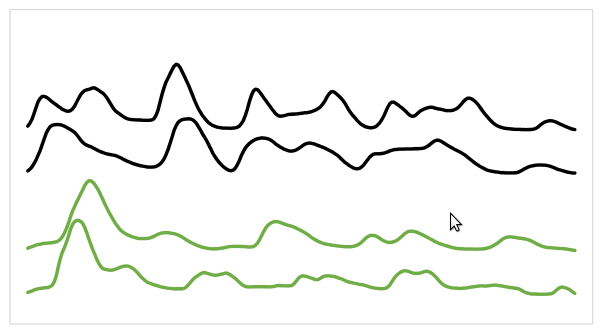
\includegraphics[scale = 0.5]{caracteristiquesFiftyWordUCR.jpeg}
\caption{D\'etection du motif commun en alignant les s\'eries. Les deux s\'eries du haut repr\'esentent la classe $30$ et les deux s\'eries du bas repr\'esentent la classe $50$.}
\label{caracteristiquesFiftyWordUCR}
\end{figure}
% ---- figure caracteristiquesFiftyWordUCR.

Les approches bas\'ees sur les vecteurs sont pertinentes quand il existe un d\'ecalage de temps entre les pics et les creux des s\'eries, comme c'est le cas avec les deux courbes du bas dans la figure \ref{caracteristiquesFiftyWordUCR}. 
\newline
Les m\'ethodes telles que 
{\em Time Warp Edit}, {\em Move-Split-Merge}, 
%{\em Elastic Ensemble}, {\em Collective Of Transform Ensemble} 
{\em Longest Common Subsequence } et 
{\em distance de Pearson} sont des distances de {\em mesures \'elastiques} qui se servent de l'approche vectorielle. 
Les  distances de {\em mesures \'elastiques} sont les meilleures approches pour traiter les probl\`emes des s\'eries enti\`eres \`a savoir la d\'etection de pics, de d\'ecalage et de creux entre les s\'eries.


	\subsubsection{Dynamic Time Warping  DTW}
		% ---- figure DTW
\begin{figure}[htb!] 
\centering
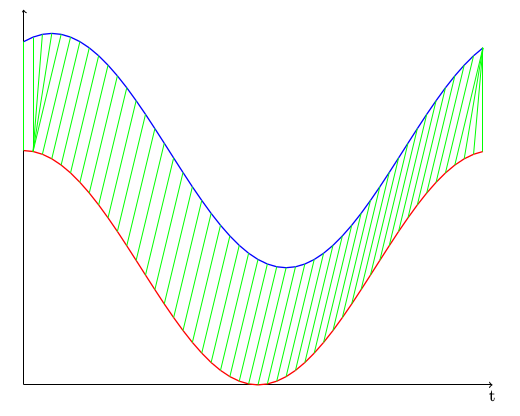
\includegraphics[scale = 0.5]{DTW2courbes.png}
\caption{Deux s\'equences en dimension $1$ align\'ees avec Dynamic Time Warping. Les coordonn\'ees de la s\'equence du haut et de celle du bas correspondent respectivement \`a
$cos(t)$ et \`a $cos(t+\alpha)$. 
Pour des questions de visualisation, la s\'equence du dessus a \'et\'e d\'ecal\'ee vers le haut lors du trac\'e. \cite{petitjean2011descriptionDTWexemple}
}
\label{DTW2courbes}
\end{figure}
% ---- figure DTW.

{\em Dynamic time warping (DTW) } est une technique pour trouver l'aligmenent optimal entre deux s\'equences d\'ependant du temps sous certaines contraintes (figure \ref{DTW2courbes}). 
Les s\'eries temporelles sont d\'eform\'ees par une transformation non-lin\'eaire de la variable temporelle, pour d\'eterminer une mesure de leur similarit\'e, ind\'ependamment de certaines transformations non-lin\'eaires du temps.
\newline
Supposons que nous souhaitons mesurer la similarit\'e entre deux s\'eries $A = (a_1, \cdots, a_m)$ et $B = (b_1, \cdots, b_m)$.
Soit $M(A,B)$ la matrice de distances entre $A$ et $B$ o\`u $M_{i,j} = (a_i - b_j)^2$.
Un chemin d'alignement {\em Dynamic Time Warping (DTW)} est une m\'ethode inspir\'ee de la distance de {\em Levenshtein}, \'egalement appel\'e {\em distance d'\'edition}. \`A l'origine, {\em DTW} \'etait appliqu\'e  dans le domaine de la reconnaissance vocale et permet de trouver l'alignement global optimal entre deux s\'equences, c'est-\`a-dire faire correspondre chaque \'el\'ement de chaque s\'equence \`a au moins un \'el\'ement de l'autre s\'equence en minimisant les co\^uts d'association. 
Le co\^ut d'une association correspond \`a la distance entre les deux \'el\'ements; classiquement une $l_p$ norm \cite{chen2004marriageLpNorm}.
La figure \ref{DTW2courbes} repr\'esente un exemple d'alignement op\'er\'e par {\em DTW}.
Il illuste l'alignement de deux sinusoides l\'eg\`erement d\'ephas\'ees. Le r\'esultat num\'erique fournit par {\em DTW} correspond \`a la somme des hauteurs des ``barreaux'' form\'es par les associations. Les extr\'emit\'es des alignements de la figure \ref{DTW2courbes} montrent que {\em DTW} est capable de r\'ealigner correctement une s\'equence par rapport \`a une autre, et parvient ainsi \`a saisir des similarit\'es que la
distance euclidienne ne peut extraire.
\newline
La distance {\em Dynamic Time Warping} est d\'efinie r\'ecursivement par :
$$
D(A_i, B_j) = \delta(A_i,B_j) + min
				\begin{cases}
				D( A_{i-1}, B_{j-1}), \\
				D( A_{i}, B_{j-1}), \\
				D( A_{i-1}, B_{j}))
				\end{cases}
$$
o\`u $A_i$ repr\'esente la sous-s\'equence $(a_1, \cdots, a_i)$. 
Le co\^ut de l'alignement optimal est alors donn\'e par
$ D(A_{|A|}, B_{|B|})$.
Le principe de programmation dynamique peut alors se r\'esoudre par un arbre en partant des
feuilles en supposant que le probl\`eme principal peut \^etre symbolis\'e par la racine et les sous-probl\`emes par des noeuds appartenant aux diff\'erents sous-arbres.
La fonction DTW peut alors \^etre m\'emois\'ee : les diff\'erents appels peuvent \^etre retenus afin de ne pas calculer deux fois la fonction appel\'ee avec les m\^emes param\`etres. 
Aussi est-il habituel, comme l'arbre contient
$| A | . | B |$ noeuds diff\'erents, de stocker ces diff\'erents r\'esultats interm\'ediaires dans une matrice $|A| \times | B |$.
Le calcul de $DTW$ consiste alors \`a trouver le chemin de co\^ut minimum dans la matrice, ce qui s'ex\'ecute avec une complexit\'e en temps et en m\'emoire de $\Theta(|A| \times |B|)$.

	\subsubsection{Time Warp Edit TWE}
		La distance {\em Time Warp Edit} (TWE) est une mesure de distance pour des s\'eries temporelles  discr\`etes. En comparaison avec les distances telles {\em Dynamic Time Warping (DTW)} \cite{muller2007dynamicDTW} et {\em longest common subsequence (LCS)} \cite{greenberg2002fastLCS}, la distance {\em TWE} est une m\'etrique propos\'ee par {\em P.F. Marteau} en $2009$. 
La distance {\em TWE} a quatre propri\'et\'es :
\begin{itemize}
	\item Traite le d\'ecalage temporelle local avec des performances \'elev\'ees.
	\item Satisfait l'in\'egalit\'e triangulaire c'est-\`a-dire $AB \le AC+CB$ avec $AB,AC, CB$ des cot\'es d'un triangle quelconque.
	\item Comprend le param\`etre de rigidit\'e $\nu$ qui contr\^ole l'\'elasticit\'e de la m\'etrique.
	\item Utilise la diff\'erence de temps pour comparer les segments de s\'eries temporelles comme des co\^uts de correspondances locales. 
\end{itemize}
Le param\`etre $\nu$ est important dans l'algorithme de {\em TWE} parce qu'il rend plus flexible l'identification de motifs (matching) entre les s\'eries temporelles. 
La preuve de son efficacit\'e a \'et\'e prouv\'ee dans \cite{marteau2009time}.

L'algorithme de {\em TWE} introduit trois op\'erations : $delete_A$, $delete_B$ et $match$ pour l'\'edition de deux s\'eries discr\`etes $A$ et $B$. L'\'edition d'une s\'erie temporelle consiste \`a modifier cette s\'erie en sous-ensembles de m\^emes tailles \`a partir d'une des trois op\'erations et chaque sous-ensemble est d\'esign\'e par  {\em s\'equence}. La similarit\'e entre les s\'eries $A$ et $B$ est le co\^ut minimum de s\'equences n\'ecessaire pour transformer $A$ en $B$.
En se basant sur ces trois op\'erations, l'algorithme de {\em TWE} calcule le co\^ut d'une s\'equence \`a chaque op\'eration pour toutes les paires de s\'eries avec l'\'equation \ref{coutSequenceTWE}. Dans cette \'equation, $U$ d\'esigne l'ensemble des s\'eries finies $U = \{A_1^p ~|~ p\in \N \}$ o\`u $A_1^p$ est une s\'erie avec des temps discrets variant de $1$ \`a $p$,
 $A_1^0$ est la s\'erie nulle de longueur nulle et 
 $a'_i$ d\'esigne le $i^{ieme}$ \'el\'ement de la s\'erie $A$.
Nous consid\'erons alors que $a'_i \in S \times T$ o\`u $S \subset R^d$ avec $d \ge 1$ int\`egre un espace multidimensionnel de variables et $T \subset R$  int\`egre la variable temporelle.
Ainsi, nous pouvons \'ecrire $a'_i = (a_i, t_{a_i})$, o\`u $a_i \in S$ et $t_{a_i} \in T$ avec la condition que  $t_{a_i} > t_{a_j}$ quand $i > j$ (le temps est strictement croissant dans la s\'equence des \'el\'ements).
La p\'enalit\'e not\'ee $\lambda$ est constante.
La similarit\'e entre les s\'eries $A$ et $B$ est calcul\'ee r\'ecursivement par 
\begin{equation}
	\delta_{\lambda,\nu}(A_1^p, B_1^q) = min
	\begin{cases}
		\delta_{\lambda,\nu}(A_1^{p-1}, B_1^q) + \Gamma(a'_p \rightarrow \Lambda) ~~~~~ delete_A, \\
		 \delta_{\lambda,\nu}(A_1^{p-1}, B_1^{q-1}) + \Gamma(a'_p \rightarrow b'_q) ~~~~~ match, \\
		 \delta_{\lambda,\nu}(A_1^{p-1}, B_1^q) + \Gamma(\Lambda \rightarrow a'_p) ~~~~~ delete_B, \\
	\end{cases}
	\label{coutSequenceTWE}
\end{equation} 
avec 
 \[
	\begin{array}{lcl} 
	\Gamma(a'_p \rightarrow \Lambda) & = & d(a'_p, a_{p-1}) + \lambda  \\ 
	\Gamma(a'_p \rightarrow b'_q) & = & d(a'_p, b'_{q}) + d(a'_{p-1}, b'_{q-1}) \\
	\Gamma(\lambda \rightarrow b'_q)  & = & d(b'_q, b'_{q-1}) + \lambda. 
	\end{array}
\]
La r\'ecursivit\'e est initialis\'ee par 
  \[  
 	\begin{cases}
 	\delta_{\lambda,\nu}(A_1^0, B_1^0) = 0, \\
 	\delta_{\lambda,\nu}(A_1^0, B_1^j) = \infty ~pour~ j \ge 1, \\
 	\delta_{\lambda,\nu}(A_1^0, B_0^j) = \infty ~pour~ j \ge 1,
 	\end{cases}
 \]
 avec $a'_0 = b'_0 = 0$ par convention.
 \newline
L'algorithme {\em TWE} introduit la rigidit\'e,  constante positive $\nu$, dans la d\'efinition de $\delta_{\lambda, \nu}$ en choisissant $d(a', b') = d_{LP}(a,b) + \nu \times d_{LP}(t_a,t_b)$ qui caract\'erise la rigidit\'e de $\delta_{\lambda, \nu}$.
Si $\nu = 0$ alors $\delta_{\lambda, \nu}$ est la distance de $S$ et non de $S \times T$.
Dans cette \'equation, $d_{LP}$ est la m\'etrique $l_p$ norm \cite{chen2004marriageLpNorm}.
L'expression finale de $\delta_{\lambda, \nu}$ est pr\'esent\'ee par l'\'equation \ref{tweFinalExpression}.
\begin{equation}
	\delta_{\lambda,\nu}(A_1^p, B_1^q) = min
	\begin{cases}
		\delta_{\lambda,\nu}(A_1^{p-1}, B_1^q) + \Gamma(a'_p \rightarrow \Lambda) ~~~~~ delete_A, \\
		 \delta_{\lambda,\nu}(A_1^{p-1}, B_1^{q-1}) + \Gamma(a'_p \rightarrow b'_q) ~~~~~ match, \\
		 \delta_{\lambda,\nu}(A_1^{p-1}, B_1^q) + \Gamma(\Lambda \rightarrow a'_p) ~~~~~ delete_B, \\
	\end{cases}
	\label{tweFinalExpression}
\end{equation} 
avec 
 \[
	\begin{array}{lcl} 
	\Gamma(a'_p \rightarrow \Lambda) &=& d_{LP}(a'_p, a_{p-1}) +\nu . (t_{a_p} - t_{a_{p-1}}) +\lambda \\  
	\Gamma(a'_p \rightarrow b'_q) &=& d_{LP}(a'_p, b'_{q}) + d_{LP}(a'_{p-1}, b'_{q-1}) + \nu . ( |t_{a_p} - t_{b_{q}}| +  |t_{a_{p-1}} - t_{b_{q-1}}|)  \\ 
	\Gamma( \lambda \rightarrow b'_q) &=& d_{LP}(b'_q, b'_{q-1}) + \nu . (t_{b_q} - t_{b_{q-1}}) + \lambda
	\end{array}
\]	

%\hspace{-1.2 cm}
	\subsubsection{Move-Split-Merge MSM}
		{\em Move Split Merge (MSM)} est une distance qui est bas\'ee sur le co\^ut de transformation d'une s\'erie temporelle en une autre s\'erie en utilisant une s\'equence d'op\'erations de {\em move}, {\em split} et {\em merge}.
{\em MSM} a l'avantage d'\^etre une m\'etrique et \^etre invariant au choix de l'origine de la s\'erie. 
En effet, soit $X=(x_1, \cdots,x_m)$ une s\'erie temporelle dans laquelle $x_i$ est un r\'eel. Une translation de $X$ par $t$, o\`u $t$ est aussi un r\'eel, est une transformation qui ajoute $t$ \`a chaque \'el\'ement de $X$ et produit la s\'erie $X+t = (x_1+t, \cdots,x_m+t)$. 
Si la distance $D$ est invariante au choix de l'origine alors  $D(X, Y ) = D(X + t, Y + t)$. {\em MSM} est invariante au choix de l'origine parce que toute transformation $S$ qui convertit $X$ et $Y$ convertit aussi $X+t$ en $Y+t$. 
Quant \`a la m\'etrique, elle permet l'utilisation d'un large nombre d'outils pour indexer, regrouper et visualiser des s\'eries dans des espaces vectoriels arbitraires.
\newline
Nous pr\'esentons un algorithme de complexit\'e quadratique qui calcule la similarit\'e entre deux s\'eries.
% details de l'algorithme
%----
Soient $X = (x_1, \cdots,x_m)$ et $Y = (y_1, \cdots, y_n)$ deux s\'eries temporelles. 
L'algorithme \ref{algorithmeMSM} d\'ecrit la m\'ethode dynamique de calcul de la distance entre $X$ et $Y$. Pour chaque  couple $(i,j)$ tel que $1 \le i \le m$ et $1 \le j \le n$, nous d\'efinissons $Cost(i,j)$ la distance {\em MSN} entre les $i$ premiers \'el\'ements de $X$ et les $j$ premiers \'el\'ements de $Y$. Ainsi, la distance {\em MSN} entre $X$ et $Y$ est simplement $Cost(X,Y)$.
Comme indiqu\'e dans l'algorithme \ref{algorithmeMSM}, $Cost(i,j)$ est calcul\'e r\'ecursivement en se basant sur   $Cost(i,j-1)$, $Cost(i-1,j)$ et $Cost(i-1,j-1)$.
\newline
$Cost(i,j) = min
				\begin{cases}
				Cost(i-1,j-1) + |x_i -y_j|, \\
				Cost(i-1, j) + C(x_i, x_{i-1}, y_j), \\
				Cost(i, j-1) + C(y_j, x_{i}, y_{j-1})
				\end{cases}
				$
avec 
$$
C(x_i, x_{i-1},y_j) = 
 	\begin{cases}
 	c ~si~ x_{i-1} \le x_i \le y_j ~ou~  x_{i-1} \ge x_i \ge y_j \\
 	c + min( |x_i - x_{i-1}|, |x_i -y_j| ) ~ sinon
 	\end{cases}
$$

\begin{algorithm}
\algsetup{indent=2em}
\caption{MSM(X,Y)}
\label{algorithmeMSM}
\begin{algorithmic}[1]
\REQUIRE{ s\'erie  $X=(x_1, \cdots, x_m)$}
\REQUIRE{ s\'erie $Y=(y_1, \cdots, y_n)$}
\STATE $Cost(1,1) = |x_1 - y_1|$
\FOR{ $i = 2, \cdots, m$}
	\STATE $Cost(i,1) = Cost(i-1,1) + C(x_i, x_{i-1},y_1)$
\ENDFOR
\FOR{ $j = 2, \cdots, n$}
	\STATE $Cost(1,j) = Cost(1,j-1) + C(y_j, x_{1},y_{j-1})$
\ENDFOR
\FOR{ $i = 2, \cdots, m$}
	\FOR{ $j = 2, \cdots, n$}
		\STATE $Cost(i,j) = min
				\begin{cases}
				Cost(i-1,j-1) + |a_i -b_j|, \\
				Cost(i-1, j) + C(a_i, a_{i-1},b_j), \\
				Cost(i, j-1) + C(b_j, a_{i},b_{j-1})
				\end{cases}
				$
	\ENDFOR
\ENDFOR
\RETURN{la distance MSM $D(X,Y)$ est $Cost(m,n)$.}
\end{algorithmic}
\end{algorithm}


%----
%Les exp\'erimentations r\'ealis\'ees sur $20$ datasets disponibles sur la base de donn\'ees de s\'eries temporelles {\em UCR} \cite{keogh2002UCR} montre que {\em MSM} produit le plus faible erreur de classification par rapport \`a {\em DTW} et  la {\em distance euclidienne} (voir tableau \ref{comparaison20datasetsUcr}).
%% mettre le tableau
%
%%----------------------------
%This chapter has described MSM, a novel metric for time series, that is based
%on the cost of transforming one time series into another using a sequence of individual
%Move, Split, and Merge operations. MSM has the attractive property of being both
%metric and invariant to the choice of origin, whereas DTW is not metric, and ERP
%is not invariant to the choice of origin. These properties may make MSM a more
%appealing choice, compared to existing alternatives, in various domains. Metricity, in
%particular, allows the use of a large number of existing tools for indexing, clustering
%and visualization, that have been designed to work in arbitrary metric spaces.
%We have presented a quadratic-time algorithm for computing the MSM distance
%between two time series. A large part of the paper has been dedicated to explaining
%the algorithm and proving its correctness. At the same time, despite the relatively
%complex proof, the actual algorithm is quite short and easy to implement, as shown
%on Figure 3.10, and on the implementations we have posted online.
%Experiments on all 20 datasets available at the UCR time series archive [3]
%demonstrate that, in ten of the 20 datasets, MSM produces lower nearest neighbor
%classification error rate than constrained DTW, unconstrained DTW, ERP, and the
%Euclidean distance. The fact that MSM gave the best accuracy in several datasets
%supports the conclusion that MSM is a method worth being aware of and experiment-
%ing with, in domains where practitioners currently use DTW or ERP. The attractive
%theoretical properties of MSM are an additional factor that can make MSM an ap-
%pealing choice, compared to existing alternatives.
%
%Let X = (x 1 , . . . , x m ) and Y = (y 1 , . . . , y n ) be two time series. Figure 3.10
%describes a simple dynamic programming algorithm for computing the MSM distance
%between X and Y . For each (i, j) such that 1 ≤ i ≤ m and 1 ≤ j ≤ n, we define
%Cost(i, j) to be the MSM distance between the first i elements of X and the first j
%elements of Y . This way, the MSM distance between X and Y is simply Cost(m, n).
%As the algorithm on Figure 3.10 shows, for i > 1 and j > 1, Cost(i, j) can be
%computed recursively based on Cost(i, j − 1), Cost(i − 1, j), and Cost(i − 1, j − 1). In
%this section we explain why it is correct to define the Cost function in this recursive
%manner, and we fully specify how to actually compute the Cost function.
%
%
%
%
%\noindent DEBUT\\
%\noindent 1. {\bf Si} $G$ estt isomorphe \`a un graphe double (voir figure XXX), {\bf alors} le traiter avec Verif\_correl \\
%~~\indent {\bf Sinon} \\
%~2. \indent {\bf Tant que} il existe un sommet $u$ t.q $Cliq(u) \in \{0,3\}$\\ 
%       	\indent~~~~~~{\bf Faire}\\
%~3.	       	\indent~~~~~~~~choisir $u$ de degr\'e minimum\\
%~4.       	\indent~~~~~~~~{\bf Si} $\{u\} \cup \Gamma_G(u)$ peut \^etre couvert par deux cliques $C_1$ et $C_2$ coh\'erentes,\\
%		\indent~~~~~~~~~~~~~~$C_1$ maximale et $C_2 = \emptyset$ si $Cliq(u)=3$\\
%	       	\indent~~~~~~~~~~~~{\bf alors}\\
%~5.	       	\indent~~~~~~~~~~~~~~{\bf Si } $Cliq(u) = 0$ et $C_2\neq \emptyset$ {\bf Alors} $Cliq = 3$ \\
%~6.		\indent~~~~~~~~~~~~~~{\bf Sinon Si} $Cliq = 0$ et $C_2 =  \emptyset$ {\bf Alors} $Cliq(u) = 1$\\
%~7.		\indent~~~~~~~~~~~~~~~~~~~~~~~{\bf Sinon} $Cliq(u) = 2$ 	\\
%~8.		\indent~~~~~~~~~~~~~~~~~~~~~~~{\bf FinSi}\\      	
%~9.		\indent~~~~~~~~~~~~~~{\bf FinSi}\\
%~10.		\indent ~~~~~~~~~~~~~$\epsilon_u = E(G[C_1]) \cup E(G[C_2])$\\
%~11.		\indent ~~~~~~~~~~~~~{\bf Pour tout} $w \in \Gamma_G(u)$ {\bf Faire} \\
%~12.		\indent~~~~~~~~~~~~~~~~$\alpha(w) = card\{[w,x] \in E - \epsilon_u\}$\\
%~13.		\indent~~~~~~~~~~~~~~~~{\bf Si} $\alpha_w > 0$ {\bf Alors}\\
%~14.		\indent~~~~~~~~~~~~~~~~~~{\bf Si} $Cliq(w) = 0$ {\bf Alors} $Cliq(w) =3$\\
%~15.		\indent~~~~~~~~~~~~~~~~~~{\bf Sinon Si} $Cliq(w) = 3$ {\bf Alors} $Cliq(w) =-1$\\
%~16.		\indent~~~~~~~~~~~~~~~~~~{\bf FinSi} \\
%~17.		\indent~~~~~~~~~~~~~~~~{\bf Sinon Si} $Cliq(w) = 0$ {\bf Alors} $Cliq(w) =1$\\
%~18. 	\indent~~~~~~~~~~~~~~~~~~~~~~~~~{\bf Sinon Si} $Cliq(w) = 3$ {\bf Alors} $Cliq(w) = 2$ \\
%~19. 	\indent~~~~~~~~~~~~~~~~~~~~~~~~~{\bf FinSi} \\
%~20.		\indent ~~~~~~~~~~~~~{\bf FinPourTout}\\
%~21.		\indent ~~~~~~~~~~~~~$E = E - \epsilon_u$\\
%~22.		\indent            ~~~~~~~{\bf Sinon} $Cliq(u) = -1$\\
%	       	\indent~~~~~~~~~~~~{\bf FinSi}\\
%       	\indent~~~~~~
%~23. \indent {\bf FinTant que}\\
%~24. \noindent {\bf Fin Si}\\
%\noindent FIN\\
	\subsubsection{Distance de Pearson}
		Dans la comparaison de s\'eries temporelles, nous avons toujours constat\'e que la normalisation dans le calcul d'une distance euclidienne entre des s\'eries donne de meilleurs r\'esultats.
Nous allons montrer la relation existante entre la distance euclienne et le coefficient de Pearson.
\newline
Soient deux s\'eries temporelles $A$ et $B$ compos\'ees de $T$ \'el\'ements $A=(a_1, \cdots, a_T) ~et~ B=(b_1, \cdots, B_T)$.
La distance euclidienne entre  $A$ et $B$ est d\'efinie par l'\'equation \ref{distanceEuclienne}
\begin{equation}
\label{distanceEuclienne}
d_E = \sum_{t=1}^{T}(a_i - b_i)^{2}
\end{equation}
Elle est une m\'etrique et les s\'eries $A$ et $B$ sont identiques si cette distance est \'egale \`a $0$. Pour les analyses de s\'eries, il est recommand\'e de normaliser les s\'eries pour \'eviter les variations d'\'echelles.
En ce qui concerne le coefficient de Pearson, il mesure la corr\'elation $\varrho$  entre deux variables al\'eatoires $X$ et $Y$ comme indiqu\'e dans l'\'equation \ref{coeffPearson}.
\begin{equation}
\label{coeffPearson}
 \varrho_{X,Y} = \frac{ E[X - \mu_{X}][ Y - \mu_{Y}] }{\sigma_X . \sigma_Y} 
\end{equation}
o\`u $\mu_{X}$ est la moyenne  et $\sigma_{X}$ est l'\'ecart-type de $X$.
Le coefficient $|\varrho| = 1$ est \'egal \`a  
$1$ si les variables $X$ et $Y$ sont parfaitement corr\'el\'ees et 
$0$ si $X$ et $Y$ sont non corr\'el\'ees.
\newline
Dans le but d'utiliser le coefficient de Pearson comme une distance de s\'eries temporelles, nous introduisons la {\em distance de Pearson} en g\'en\'erant de petites valeurs de distances pour des s\'eries similaires. %corr\'el\'ees. 
Elle est d\'efinie par l'\'equation \ref{personDistance}.
\begin{equation}
\label{personDistance}
d_{P}(A,B) = 1 - \varrho_{A,B}= 1- \frac{ \frac{1}{T} \sum_{t=1}^{T} (a_t - \mu_A)(b_t - \mu_B) }{\sigma_A . \sigma_B}
\end{equation}
avec $0 \le d_P{(A,B)} \le 2$.
Nous obtenons une parfaite correspondance ($d_P = 0$) pour les s\'eries $A$ et $B$ s'il existe des nombres $\alpha, \beta \in \R$ avec $\beta>0$ tels que $a_i = \alpha + \beta * b_i$.
Nous exprimons $d_E$ en fonction de $d_P$.
\begin{equation}
\label{demontrationPearson}
d_E(A,B) = \sum_{t=1}^{T}(a_i - b_i)^{2}
=  \sum_{t=1}^{T}(a_i - 0)^{2} -2 \sum_{t=1}^{T}(a_i . b_i) + \sum_{t=1}^{T}(b_i - 0)^{2}
\end{equation}
Les termes $ \sum_{t=1}^{T}(a_i - 0)^{2}$ et $\sum_{t=1}^{T}(b_i - 0)^{2}$ correspondent \`a l'\'ecart-type des s\'eries $A$ et $B$ en supposant que la moyenne de ces s\'eries est nulle $\mu_{A} = \mu_{B} = 0$ et leurs \'ecarts-types sont \'egaux \`a $1$ ($\sigma_A = \sigma_B = 1$).
L'\'equation pr\'ec\'edente \ref{demontrationPearson} devient 
$$
d_E(A_{norm},B_{norm}) = 2.T (1 - \frac{\frac{1}{T} \sum_{t=1}^{T}(a_{i,norm} - 0)(b_{i,norm} - 0) }{1 . 1})
= 2 . T. d_P(A_{norm},B_{norm})
$$
Ainsi, la distance euclidienne de deux s\'eries norm\'ees est \'egale \`a la distance de Pearson multipli\'ee par un facteur constant $2T$.
L'\'equivalence entre ces deux distances est pertinente parce que certains algorithmes utilisent  la distance  euclidienne pour faire de la classification (cas de k-means). 
Dans l'article \cite{berthold2016clusteringDistancePearson}, l'auteur utilise la classification {\em k-means} de s\'eries avec la distance de Pearson et il en conclut que cette classification donne les m\^emes  r\'esultats que le {\em k-means} avec la distance euclidienne.
	\subsubsection{Longest Common Subsequence}
		La distance {\em longest common subsequence (LCSS)} est bas\'ee sur la reconnaissance de motifs dans les probl\`emes {\em (LCSS}) . Dans ces probl\`emes, il recherche la plus longue s\'equence qui est commune aux deux s\'eries discr\`etes en utilisant la distance {\em edit distance (ED)}.
Cette approche a \'et\'e \'elargie aux s\'eries continues en d\'efinissant la variable de seuil $\epsilon$ qui indique la diff\'erence entre une paire de valeurs. Cette diff\'erence d\'etermine s'il existe une similarit\'e entre ces s\'eries. 
{\em LCSS} trouve un alignement optimal entre deux s\'eries en ins\'erant des \'ecarts pour d\'eterminer le nombre maximum de paires correspondantes.
La distance {\em LCSS} entre deux s\'eries $A$ et $B$ peut \^etre calcul\'ee \`a partir de l'algorithme \ref{algorithmeLCSS}.
 
\begin{algorithm}
\algsetup{indent=2em}
\caption{LCSS(A,B)}
\label{algorithmeLCSS}
\begin{algorithmic}[1]
\STATE{Soit $L$ une matrice initialis\'ee \`a $0$ de dimension $(m+1) \times (m+1)$}
\FOR{$i \leftarrow m ~ a ~ 1$}
	\FOR{$j \leftarrow m ~ a ~ 1$}
		\STATE{$L_{i,j} = L_{i+1, j+1}$}
		\IF{$a_i =  b_j$}
			\STATE{$L_{i,j} \leftarrow L_{i, j} + 1$}
		\ELSIF{$ L_{i,j+1} > L_{i,j}$}
			\STATE{$ L_{i,j} \leftarrow  L_{i,j+1}$ }
		\ELSIF{ $L_{i+1,j} > L_{i,j}$ }
			\STATE{ $L_{i,j} \leftarrow L_{i+1,j}$ }
		\ENDIF
	\ENDFOR
\ENDFOR
\RETURN{$L_{1,1}$}
\end{algorithmic}
\end{algorithm}

La distance {\em LCSS} entre les s\'eries $A$ et $B$ est 
$$
d_{LCSS}(A,B) = 1 - \frac{LCSS(A,B)}{m}
$$
%The LCSS distance is based on the solution to the LCSS problem in pattern matching.
%The typical problem is to find the longest subsequence that is common to two discrete
%series based on the edit distance. An example using strings is shown in Fig. 3.
%This approach can be extended to consider real-valued time series by using a dis-
%tance threshold , which defines the maximum difference between a pair of values
%that is allowed for them to be considered a match. LCSS finds the optimal alignment
%between two series by inserting gaps to find the greatest number of matching pairs.
%	\subsubsection{Collective of Transform Ensemble COTE}
%		{\em Collective of Transform Ensemble (COTE)} se base sur deux id\'ees qui permettent la transformation des donn\'ees et am\'eliore la pr\'ecision des algorithmes de classification de s\'eries temporelles. La premi\`ere id\'ee est la transformation de nos donn\'ees dans un espace alternatif  o\`u les selections des caract\'eristiques des donn\'ees {\em features} est plus simple \`a detecter. La seconde id\'ee utilise les ensembles heterog\`enes qui produisent de meilleurs resultats qu'un re\'echantillonnage avec une apprentissage fiable.

provient de la demontration de {\em Keogh} \cite{} qui affirme que la pr\'ecision est atteinte par des ensembles de sch\'emas simples.  
{\em COTE} contient un ensemble de classifiers construit dans le domaine temporelle, frequentielle et dans la transformation de shapelets. Par exemple, COTE utilise des distances \'elastiques quand il op\`ere dans le domaine temporelle. 

it was demonstrated that with a single data representation, improved accuracy can be achieved through simple ensemble schemes. We combine these two principles to test the hypothesis that forming a collective of ensembles of classifiers on different data transformations improves the accuracy of time-series classification. The collective contains classifiers constructed in the time, frequency, change, and shapelet transformation domains.For the time domain, we use a set of elastic distance measures.
%	\subsubsection{Elastic Ensemble}
%		{\em Elastic ensemble (EE)} est une combinaison de $11$ classificateurs utilisant la m\'ethode de $k$ plus proches voisins et les distances qui se calculent sur les series enti\`eres (distance de Pearson, distance euclidienne, MSM).
Les $11$ classificateurs dans {\em EE } sont :
  
	{\bf Conclusion} : plusieurs distances ont \'et\'e pr\'esent\'ees et leur point commun est l'utilisation de toute la s\'erie pour le calcul de la similarit\'e.
Parmi ces distances, nous distinguons les distances qui sont des m\'etriques {\em TWE, MSM et la distance de Pearson} et celles qui ne le sont pas {\em LCSS et DTW}.

%s\'eries enti\`eres pour calculer leur similarit\'e dans le temps. Parmi ces distances, nous distinguons les distances qui sont des m\'etriques {\em TWE, MSM et la distance de Pearson} et celles qui ne le sont pas {\em LCSS et DTW}.

\subsection{Similarit\'e sur les s\'equences}
	Nous pr\'esentons, dans cette section,  les distances qui transforment au pr\'ealable les s\'eries pour comparer leurs caract\'eristiques. Ces caract\'eristiques sont appel\'ees des { \em features}. 
\newline
Pour mesurer la similarit\'e entre des s\'eries temporelles, des m\'ethodes proposent de repr\'esenter les donn\'ees en sous-s\'equences diff\'erentes, chacune formant une classe. Cette transformation est d\'esign\'ee par {\em shapelets}. Un shapelet consid\`ere que les sous-s\'equences sont ind\'ependantes. 
Le calcul de similarit\'e entre des s\'eries se produit localement entre les s\'equences de m\^eme phase au moyen d'une m\'etrique. G\'en\'eralement la m\'etrique utilis\'ee est la distance euclidienne. 
D'abord, les shapelets g\'en\'eralisent l'algorithme des $k$ plus proche voisins ({\em k-means}) largement utilis\'e dans les arbres de d\'ecision pour am\'eliorer les classifications \cite{wang2013experimental}. Ensuite, ils sont interpr\'etables et donnent une id\'ee de la diff\'erence entre deux classes \cite{ye2011time}. Enfin, ils peuvent \^etre aussi plus  pr\'ecis que d'autres m\'ethodes concurrentes \cite{mueen2011logical, ye2011time}.
\newline 
{\em Hills et al.} \cite{hills2014classificationShapelets} propose l'algorithme \ref{algoTransformShapelets} de transformation de s\'eries  en {\em shapelets} en retournant les $k$ premiers shapelets dans une seule ex\'ecution.
L'algorithme \ref{algoTransformShapelets} se d\'ecrit comme suit :
Soient $w_i$ une sous-s\'erie d'une s\'erie temporelle $A$ avec $i \le k$ et $W_l$ l'ensemble de taille $l$ de s\'eries $w_i$.
La distance de {\em shapelet}  $sDist(S, T)$ entre un shapelet $S$ et une s\'erie $T$ est la distance euclidienne minimum entre $S$ et $w_i \in W_l$.
$$
sDist(S, T) = min_{w_i \in W_l} (dist(S, w_i))
$$
Le meilleur shapelet a une distance $sDist$ faible pour les instances d'une classe et des distances $sDist$ \'elev\'ees pour les instances des autres classes.
\newline
Nous consid\'erons $w_i$ comme un {\em shapelet candidat}. L'ensemble de valeurs de $sDist$ pour chaque candidat est trouv\'e en utilisant la fonction {\em findDistances} et est \'evalu\'e par la proc\'edure {\em assessCandidate} au moyen de la mesure $f-statistic$. 
Les $k$ meilleurs shapelets sont retourn\'es apr\`es la suppression des sous-s\'eries candidats par la fonction {\em removeSelfSimilar}.
Nous nous servons de la proc\'edure d'estimation de longueur, d\'ecrite dans \cite{lines2012shapelet}, pour trouver les valeurs appropri\'ees \`a utiliser comme les longueurs maximales et minimales de shapelets. 
Nous g\'en\'erons un maximum de $k=10n$ shapelets o\`u $n$ est la taille de la s\'erie initiale.
\newline
Nous transformons la s\'erie initiale  en utilisant les meilleurs shapelets comme des features o\`u 
$sDist(S_i, T_j)$ d\'esigne l'\'el\'ement $i$ dans l'instance $j$ de la s\'erie transform\'ee, 
$S_i$ est le $i^{ieme}$ shapelet et $T_j$ est la $j^{ieme}$ instance dans la s\'erie initiale.
La complexit\'e de l'algorithme  est de ${\cal O}(n*m^2)$ avec 
$n$ le nombre de s\'eries temporelles et
$m$ la plus longue s\'erie temporelle \cite{rakthanmanon2013fast}.
\begin{algorithm}
\algsetup{indent=2em}
\caption{ShapeletSelection(T,min,max,k)}
\label{algoTransformShapelets}
\begin{algorithmic}[1]
\STATE $kShapelets \leftarrow \emptyset$
\FOR {all $T_i$ in T}
	\STATE $shapelets \leftarrow \emptyset$
	\FOR {$l \leftarrow min ~\TO~max $}
		\STATE $W_{i,l} \leftarrow generateCandidates(T_i,l)$
		\FOR { all subsequence S $ \in W_{i,l}$ }
			\STATE{$D_S \leftarrow findDistances(S,T)$}
			\STATE{$quality \leftarrow assessCandidate(S, D_S)$}
			\STATE{shapelets.add(S, quality)}
		\ENDFOR
	\ENDFOR
	\STATE{sortByQuality(shapelets)}
	\STATE{removeSelfSimilar(shapelets)}
	\STATE{$kShapelets \leftarrow merge(k, kShapelets, shapelets)$}
\ENDFOR
\RETURN{kShapelets}.
\end{algorithmic}
\end{algorithm}
\newline 

{\bf Conclusion} : les shapelets transforment la s\'erie en un sous-ensembles de s\'equences avec la fonction {\em generateCandidate}. Chaque s\'equence d'une s\'erie est nomm\'ee {\em shapelet candidat} et ce {\em shapelet candidat} est compar\'e avec  les autres shapelets candidat de la m\^eme s\'erie \`a partir \`a la {\em distance de shapelet}. Une fois les {\em shapelets candidats} de chaque s\'erie s\'electionn\'ee avec l'algorithme {\em ShapeletSelection}, on les compare avec la distance euclidienne.
Cette m\'ethode est inefficace pour des s\'eries de grande taille.
%We transform the original data using the best shapelets as
%features, where attribute i in instance j of the transformed
%data is sDist(S i , T j ) , where S i is the i th best shapelet and
%T j is the j th instance of the original data.
%
%It makes a single
%pass through the original data, taking each subseries of each
%series as a shapelet candidate. The set of sDist values for
%each candidate is found using f indDistances and assessed
%using the f-stat quality measure in the assessCandidate
%procedure. The best k shapelets are returned, after removing
%overlapping candidates in the method removeSelf Similar .
%We use the length estimation procedure described in [23] to
%determine the appropriate values to use as the minimum
%and maximum shapelet lengths, and generate a maximum
%of k = 10n shapelets, where n is the size of the training set
%of the original data.
%
%
%One benefit of the shapelet approach is that shapelets are comprehensible, and can offer insight into the problem domain. The original shapelet-based classifier embeds the shapelet-discovery algorithm in a decision tree, and uses information gain to assess the quality of candidates, finding a new shapelet at each node of the tree through an enumerative search. 
%
%Shapelets are time series
%subsequences selected (or learned) so as to discriminate classes. Amongst these
%approaches,  the  Shapelet  Transform  (ST)  [6]  uses  shapelets  as  surrogates  for
%representing time series: each time series is projected against the set of shapelets,
%resulting in a vector in which components represent the distances between the
%time series and the shapelets.
\subsection{Similarit\'e par aggr\'egation des caract\'eristiques descriptives}
	Les mod\`eles de classification de s\'eries temporelles bas\'es sur des caract\'eristiques
descriptives  supposent  d'extraire  un  ensemble  de  caract\`eres qu'on  esp\`ere  \^etre
repr\'esentatif de la forme g\'en\'erale d'une s\'erie temporelle. Le plus commun\'ement,
ces caract\`eres sont quantifi\'ees pour former des "sacs de mots" (BoW pour "Bag of Words'').
Dans la r\'ecup\'eration d'information, l'approche {\em BoW} d'estimation de la fr\'equence des mots en ignorant leur localisation est tr\`es commune. L'id\'ee est d'estimer la fr\'equence d'occurences des caract\`eres des s\'eries puis  d'utiliser ces fr\'equences comme des ``features'' pour faire de la  classification.
\newline
Les approches suivantes diff\`erent uniquement par les caract\'eristiques extraites.
En effet, l'approche {\em Bag Of Pattern (BOP)} \cite{lin2012rotation} convertit la s\'erie temporelle en une s\'erie discr\`ete gr\^ace \`a la m\'ethode {\em Symbolic Aggregate approXimation (SAX)} \cite{lin2007experiencing}. Il cr\'ee un ensemble de mots {\em SAX} pour chaque s\'erie par l'application d'une fen\^etre glissante, puis se sert de la fr\'equence des mots dans la s\'erie comme sa nouvelle caract\'eristique. 
{\em Baydoyan et al.} \cite{baydogan2013bag} d\'ecrit l'approche {\em bag-of-features} qui combine les caract\'eristiques de fr\'equences et d'intervalles. L'algorithme appel\'e {\em time series based on bag-of-features representation (TSBF)} implique la s\'eparation entre la cr\'eation de features et les \'etapes de classification. 
La cr\'eation de features implique la g\'en\'eration d'intervalles al\'eatoires et les features repr\'esentent, g\'en\'eralement, la moyenne, la variance et la pente sur un intervalle. 
Le d\'ebut et la fin d'un intervalle sont incluses dans les features. 
\subsection{Conclusion sur les m\'ethodes de similarit\'e}
	Dans cette partie, nous avons \'enum\'er\'e les diff\'erentes m\'ethodes (distances) que nous pouvons utiliser pour calculer la similarit\'e entre des s\'eries. Nous avons cat\'egoris\'e les distances en deux groupes : 
celles qui n'apportent aucune modification aux s\'eries et 
celles qui transforment les s\'eries avant de d\'ebuter l'analyse. 
La transformation des s\'eries se fait de deux mani\`eres. La premi\`ere consiste \`a diviser la s\'erie en s\'equences et \`a supposer que chaque s\'equence est ind\'ependante des autres. 
Quant \`a la seconde, elle consiste \`a remplacer la s\'erie par certaines caract\'eristiques descriptives telles que la moyenne, l'\'ecart-type, l'encodage de la s\'erie par des mots. 
Parmi celles qui ne modifient pas les s\'eries, nous distinguons certaines qui ont la propri\'et\'e de m\'etriques. 
%Elle signifie que la distance entre la serie A et B est la meme que la distance entre B et A. 
Cette propri\'et\'e est importante pour choisir la m\'ethode de calcul de la similarit\'e entre des s\'eries.   

\section{M\'ethode de similarit\'e entre des mesures \'electriques : \\ distance de Pearson}
	\subsection{Choix de la distance}
		%% kel est le but de notre etude, kest ce qu'on recherche lorsqu'on compare 2 series.
%%%nous recherchons * la propagation des changements de regimes dans le reseau electrique. cela signifie que la consommation de puissance d'un noeud baisse quand les \'equipements qu'il alimente sont \`a l'arr\^et. * les arcs rattach\'es aux m\^emes noeuds doivent avoir les m\^emes profils de consommation.
%Nos s\'eries temporelles ont la particularit\'e d'\^etre des mesures \'electriques. Pour certaines grandeurs comme la puissance ou l'intensit\'e, les mesures se propagent dans l'ensemble du r\'eseau en suivant la loi de conservation \cite{loiDeConservation} ainsi que les changements de r\'egimes de consommation qui font apparaitre des pics dans les courbes des s\'eries temporelles. En d'autres termes, les arcs rattach\'es aux m\^emes noeuds doivent avoir les m\^emes {\em profils de consommation}. Le {\em profil de consommation} d'un arc est la variation, dans le temps, de la quantit\'e d'\'energie en fonction de l'\'etat de fonctionnement de l\'equipement auquel cet arc est rattach\'e et qui l'alimente. Cela signifie que la consommation en puissance d'un noeud
% baisse quand les \'equipements qu'il alimente sont \`a l'arr\^et ou 
% augmente quand des \`equipements se mettent en marche.
%La mesure de similarit\'e devra determiner les arcs partageant un noeud ou les series qui ont les memes profils de consommation
%La distance de similarit\'e entre des paires de s\'eries calcule un coefficient qui compare les profils de consommation des arcs dont proviennent les s\'eries. Des s\'eries qui ont les m\^emes profils doivent avoir la distance la plus \'elev\'ee (c'est-\`a-dire $1$) et celles qui ont des profils diff\'erents ont la distance la plus faible (c'est-\`a-dire $0$).

%------------ % kel est le but de notre etude, kest ce qu'on recherche lorsqu'on compare 2 series.
Nos s\'eries temporelles ont la particularit\'e d'\^etre des mesures \'electriques. Ces s\'eries sont associ\'ees aux arcs entrants dans des \'equipements. Pour certaines grandeurs comme la puissance ou l'intensit\'e, les mesures se propagent dans l'ensemble du r\'eseau en suivant la loi de conservation \cite{loiDeConservation}. 
Cela implique que toute variation de consommation \'electrique des \'equipements apparait dans les courbes des s\'eries temporelles comme des pics. Cela signifie que la consommation en puissance d'un \'equipement
 baisse quand les \'equipements qu'il alimente sont \`a l'arr\^et ou 
 augmente quand ces \'equipements se mettent en marche.
Nous d\'esignons la courbe d'une s\'erie temporelle par le {\em profil de consommation} d'un arc. 
%Le profil de consommation d'un arc est la variation, au cours du temps, de la quantit\'e d'\'energie qui circule dans l'arc.
Ainsi, nous supposons que les arcs rattach\'es aux m\^emes \'equipements ont les m\^emes profils de consommation.
N\'eammoins, des arcs appartenant \`a la chaine de propagation de l'\'electricit\'e (c'est-\`a-dire tous les arcs par lesquels l'\'electricit\'e transite) n'ont pas les m\^emes profils car certains \'equipements sont rattach\'es \`a deux sources d'\'energies et les pics s'attenuent durant la propagation.
{\em La distance de similarit\'e entre des paires de s\'eries calcule le coefficient de similarit\'e qui compare les profils de consommation des arcs}. Des arcs ont les m\^emes profils  si et seulement si le coefficient de similarit\'e est le plus \'elev\'e (c'est-\`a-dire $1$) et ont des profils diff\'erents si  leur coefficient est le plus faible (c'est-\`a-dire $0$).
%------------
\newline

Le choix de notre m\'ethode de calcul de similarit\'e d\'epend des donn\'ees que nous avons collect\'ees. En effet, dans ces donn\'ees, certains arcs n'ont pas de mesures associ\'ees \`a des grandeurs physiques. Chaque valeur dans une s\'erie est la moyenne des valeurs sur un intervalle de $10$ minutes. 
Il existe aussi des valeurs manquantes dans certaines s\'eries de mesures. Nous avons attribu\'e \`a ces valeurs manquantes la moyenne des valeurs \`a leur voisinage. Cette interpolation pose probl\`eme dans le calcul de similarit\'e avec les {\em shapelets}.
 En effet, \'etant donn\'e le shapelet candidat contenant des valeurs extrapol\'ees, la correspondance entre le shapelet candidat et toutes autres s\'equences est fortement d\'egrad\'ee \`a cause des valeurs extrapol\'ees qui augmentent la distance euclidienne entre elles. Ensuite, il s'ex\'ecute lentement sur de grands ensembles de donn\'ees. Enfin le shapelet candidat est de longueur quelconque et sa d\'etermination passe par la g\'en\'eration de toutes les shapelets possibles. 
 Ce qui conduit \`a une complexit\'e de ${\cal O}(m^2)$, avec $m$ la taille de la longue s\'erie temporelle. 
% Cela rend le calcul impossible quand  notre ensemble de donn\'ees est de dimension $30 * 4320$ avec $30$ le nombre de s\'eries temporelles et $4320$ le taille d'une s\'erie temporelle.
 Cela rend le calcul irr\'ealisable pour notre ensemble de donn\'ees de dimension $30 * 4320$ avec $30$ le nombre de s\'eries temporelles et $4320$ le taille d'une s\'erie temporelle.
\newline

% incinvenient avec les sax, bop 
Par ailleurs, les m\'ethodes par aggr\'egation des caract\'eristiques descriptives fournissent \'egalement des r\'esultats mitig\'es. Prenons l'exemple de m\'ethodes de similarit\'e avec {\em Symbolic Aggregate approXimation}(SAX). Elle consiste \`a subdiviser chaque s\'erie en $M$ s\'equences de taille identique puis \`a encoder chaque s\'equence par une lettre alphab\'etique, chaque lettre \'etant choisie dans un alphabet de lettres pr\'ed\'efinies. La transformation d'une s\'equence en une lettre s'obtient gr\^ace \`a une repr\'esentation {\em PAA (Piecewise Aggregate Approximation)} et \`a une table de correspondance entre l'alphabet. 
La repr\'esentation {\em PAA} \cite{paatheorique} d'une s\'equence est la moyenne des valeurs de la s\'equence. La table de correspondance contient la liste ordonn\'ee des points appel\'es {\em breakpoints} dont chaque valeur est une division arbritraire de la distribution gaussienne en zones \'equiprobables \cite{lin2003symbolic} et un alphabet. Et \`a chaque point de la liste {\em breakpoints}, une lettre lui est associ\'ee.
La transformation de cette repr\'esentation en lettres a une complexit\'e de  ${\cal O}(mM)$ \cite{lin2003symbolic} avec $M$ est le nombre de s\'equences de la s\'erie
et $m$ la taille de la s\'erie.
Le principal inconv\'enient provient de  l'erreur produite lors de transformation. L'encodage consid\'er\'e par {\em SAX} est celui qui minimise cette erreur.
 Ainsi, une s\'erie peut avoir deux encodages diff\'erents si nous changeons l'origine des s\'equences. L'encodage n'est donc pas unique.
De m\^eme, il est difficile de d\'etecter les variations dans la s\'erie avec l'encodage {\em SAX} car  toute variation faible mais continue dans le temps a le m\^eme encodage.  Par contre, une variation forte dans la s\'erie ne modifie pas l'encodage dans le {\em breakpoint} puisque la distance {\em PAA} est la moyenne des valeurs dans la s\'equence. 
\newline

% prkoi choisir DistPearson par rapport a DTW, TWE et MSM et LCSS
Enfin, les m\'ethodes de similarit\'e, dont le r\'esultat est le moins impact\'e par les valeurs extrapol\'ees et les profils de consommation, sont celles qui utilisent l'int\'egralit\'e de s\'eries temporelles. \`A cet effet, la fen\^etre glissante de $6$ (correspondant \`a une heure) permet d'abord d'attribuer des valeurs aux instants $t$ ayant des valeurs manquantes puis de supprimer des petites variations qui peuvent p\'enaliser nos similarit\'es et enfin de mettre en \'evidence les fortes variations dans la s\'erie.
Parmi les distances \'enum\'er\'ees dans la section \ref{seriesEntieres}, nous avons d\'ecid\'e de choisir la {\em distance de Pearson} comme m\'ethode de calcul du coefficient de  similarit\'e entre les s\'eries temporelles  pour les raisons suivantes :
\begin{itemize}
	\item La distance de Pearson est une m\'etrique alors que {\em DTW} ne l'est pas. Toutefois, ces distances ne respectent pas l'in\'egalit\'e triangulaire.
	\item La classification par la m\'ethode de {\em k-means} avec la distance euclidienne produit les m\^emes r\'esultats que celle avec la distance de Pearson \cite{berthold2016clusteringDistancePearson}. {\em k-means} est une classification de r\'eference dans les bases de donn\'ees {\em UCR} \cite{keogh2002UCR} 
	\item Elle est de complexit\'e {\em lin\'eaire} alors que la complexit\'e de la distance {\em MSM} est quadratique.
	\item Elle ne traite pas de d\'ecalage entre les s\'eries comme {\em TWE}. Le traitement du d\'ecalage entre les s\'eries n'est pas n\'ecessaire puisque les s\'eries sont moyenn\'ees sur $10$ minutes et les possibles valeurs d\'ecal\'ees ont d\'ej\`a \'et\'e moyenn\'ees. De m\^eme, nous ne sommes pas parvenus \`a trouver une valeur de rigidit\'e $\nu$ correcte pour {\em TWE} \`a cause des probl\`emes dans le dataset de {\em Champlan} (valeurs manquantes et incorrectes). 
	\item La distance de Pearson n\'ecessite que les s\'eries soient normalis\'ees. Les coefficients de Pearson d\'esignent les similarit\'es entre des paires de s\'eries normalis\'ees et ils appartiennent \`a l'intervalle $[0,1]$.  Si le coefficient est \'egal \`a $1$ alors il existe une forte similarit\'e entre les s\'eries. Cependant, il n'existe pas de similarit\'e si le coefficient est  \'egal \`a $0$.
\end{itemize}


{\bf Conclusion} : 
La distance de Pearson est la mieux adapt\'ee aux calculs des coefficients de similarit\'e entre des s\'eries parce qu'elle est une m\'etrique, de complexit\'e lin\'eaire, d\'etecte les variations simultan\'ees (faibles et fortes) entre des paires de s\'eries. Toutefois, elle ne respecte pas l'in\'egalit\'e triangulaire et n\'ecessite que les donn\'ees soient normalis\'ees. Elle est donc une bonne m\'etrique pour comparer les profils de consommation.
%	\subsection{Calcul de la distance}
%		\input{calculDistance}
	\subsection{R\'esultats sur des donn\'ees r\'eelles}
		%quel est la grandeur quon a selectionne
%travailler sur un sous graphe de champlan why 
%	presentation de champlan dans le chapitre precedent
%	description du reseau de champlan et presentation du reseau (affichage) 
% calcul des coefficient de similarite
%representation de la matrice de correlation
%comparer les faux positfs avec les faux negatifs 
%choix du seuil ou de epsilon
%conclusion

% 0 - description de champlan dans le chapitre precedent
% 1 - grandeur selectionnee
%% -----
%---lien sur relation entre correlation Pearson et taille de l echantillon https://www.researchgate.net/post/What_is_the_minimum_sample_size_to_run_Pearsons_R


%  ------ chapitre precedent
%Nous avons les tensions triphas\'ees $U_{12}, U_{23}, U_{13}$, les intensit\'es triphas\'ees 
%$I_{12}, I_{23}, I_{13}$, les puissances active $P$, apparente $S$ et reactive $Q$, le  facteur de puissance $FP$ ou $cos \phi$, l'intensit\'e $I$, la tension $U$.
%Nous constatons qu'il existe deux syst\`emes de fonctionnement : le syst\`eme triphas\'e regroupant les grandeurs $U_{12}, U_{23}, U_{13}, I_{12}, I_{23}, I_{13}$ et le syst\`eme monophas\'e regroupant les grandeurs $I,U$. Les autres grandeurs sont communes aux deux syst\`emes (les grandeurs $P, Q, S, cos \phi$).
%Le syst\`eme triphas\'e est utilis\'e des sources \'electriques jusqu'aux diff\'erents tableaux \'electriques parce que le triphas\'e permet de transporter beaucoup d'\'energies.
%Quant au syst\`eme monophas\'e, il est utilis\'e des tableaux \'electriques jusqu'aux baies serveurs. Les baies sont des armoires qui alimentent plusieurs serveurs.
%  ------ chapitre precedent
Nous pr\'esentons les r\'esultats obtenus avec la distance de Pearson.
\newline
Les grandeurs physiques collect\'ees proviennent du {\em datacenter Champlan} sont au nombre de $10$. Elles sont regroup\'ees dans les syst\`emes triphas\'e et monophas\'e.
Dans les s\'eries de mesures  provenant des arcs en triphas\'e, nous remarquons qu'il y'a toujours des mesures sur une phase et les autres phases ne contiennent aucune mesure. Il n'y a aucune mesure sur deux phases simultan\'ement et lorsqu'il  existe des mesures, les $i$ premi\`eres mesures sont sur la phase $1$, les $n-i$ mesures sont sur la phase $2$. 
Les autres grandeurs ne contiennent des mesures 
soit dans les $i$ premiers instants de temps, 
soit dans les $n-i$ derniers instants de temps. 
Il est alors difficile d'exploiter ces mesures partielles.
% parler du seule tgbt qui est en monophas\'e
Quant au syst\`eme monophas\'e, $20\%$ des mesures des puissances r\'eactives $Q$ et apparentes $S$ dans une s\'erie temporelle sont manquantes, $25\%$ des mesures ne correspondent pas aux formules de calculs th\'eoriques. 
Le nombre de valeurs \`a consid\'erer dans les s\'eries des grandeurs n'est pas assez significative pour calculer les similarit\'es parce que la distance de Pearson est sensible \`a la dimension de la s\'erie \`a cause de sa relation avec le coefficient de Pearson. Il est difficile de trouver de possibles comportements identiques \`a partir des hypoth\`eses de corr\'elation avec des s\'eries de grandes tailles et autant de valeurs absentes.
\newline
% 2- description du reseau de champlan et presentation du reseau (affichage) 
Nous consid\'erons un sous-r\'eseau \'electrique de {\em Champlan} dans lequel 
\begin{itemize}
	\item La grandeur s\'electionn\'ee poss\`ede des valeurs quelque soit le syst\`eme (triphas\'e ou monophas\'e). La grandeur qui respecte cette r\`egle est la {\em puissance $P$}.
	\item Les s\'eries temporelles correspondent \`a un mois de mesures. 
		Dans chaque s\'erie, nous avons en moyenne $15\%$ de valeurs manquantes que nous remplacons par la valeur moyenne de chaque s\'erie.
	\item L'application de la loi des noeuds est possible.
	\item Aucun \'equipement n'est aliment\'e par un onduleur. La pr\'esence d'un onduleur modifie le profil de consommation d'un arc car l'onduleur recr\'ee le signal en attribuant des puissances diff\'erentes. Cela implique que nous n'avons pas des m\^emes variations.
	 
\end{itemize}
Un exemple de ce sous-r\'eseau est illustr\'e dans la figure \ref{sousReseauChamplan} dans lequel nous avons $31$ \'equipements. Les sources sont identifi\'ees par {\em TGBT} (TGBT1, TGBT2, TGBT4) et $GF$(1,2) d\'esigne le groupe froid qui g\`ere la climatisation. Les tableaux sont {\em DD205, DD206, DD105, DD106, DD108, MSC3, R486, R481, CVC1 et CVC2}. Les baies sont {\em R491, R488, R484A, R484B, R042, R483, R487, R492, R490, R493, R494}. Les onduleurs sont indiqu\'es par {\em OND} (1,2,RG). Les \'equipements {\em TGBT} sont aliment\'es par une source externe au datacenter, le fournisseur d'\'electricit\'e r\'egional {\em Enedis}.  
% ---- figure sous-reseau champlan
\begin{figure}[htb!] 
\centering
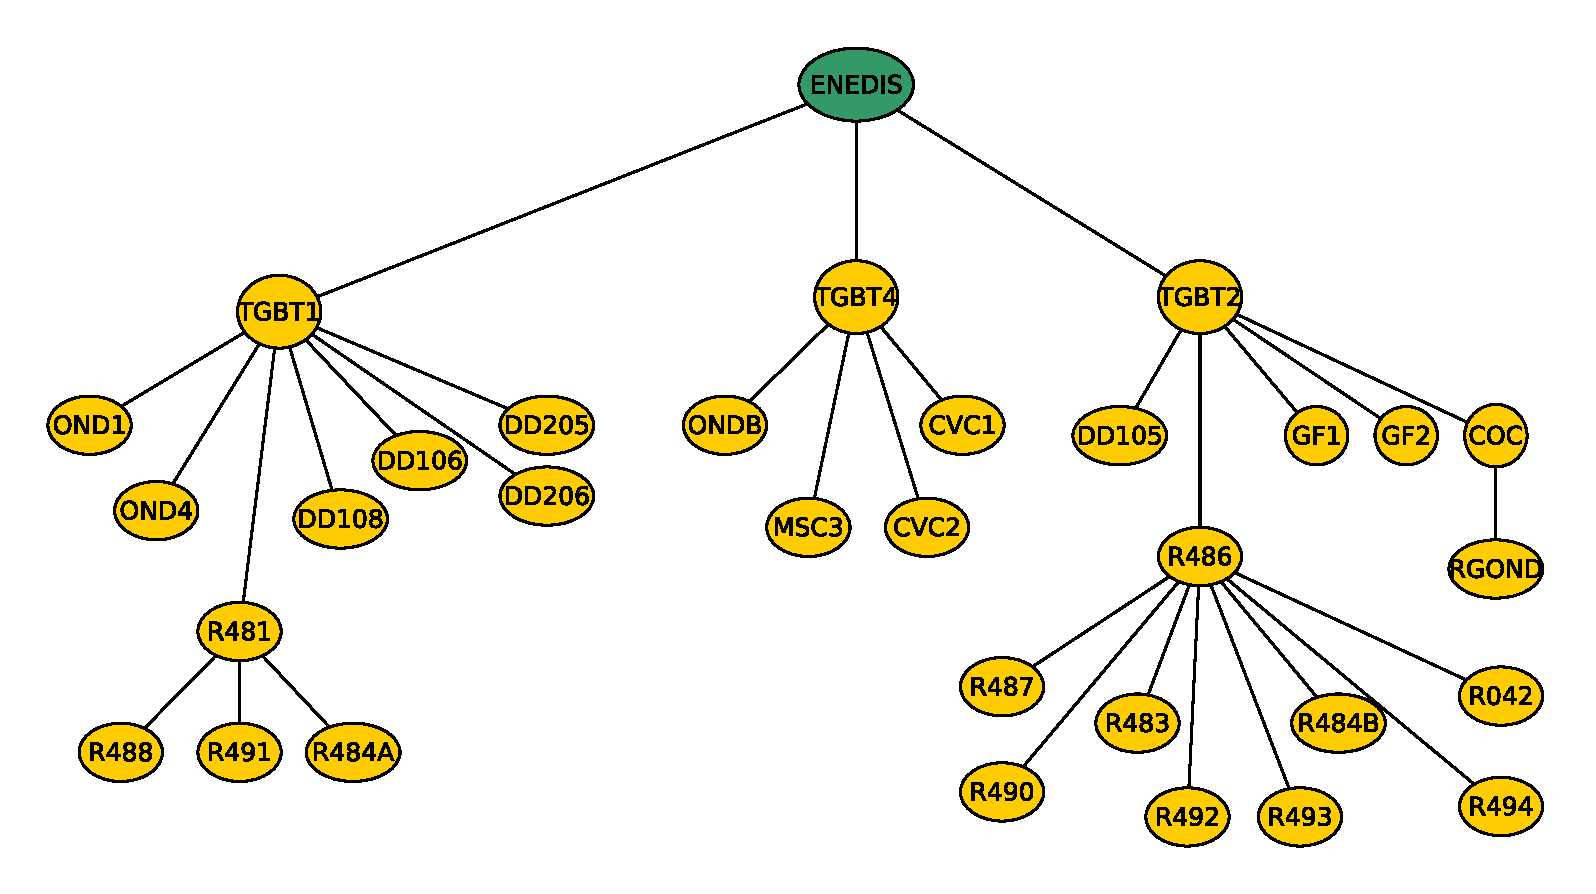
\includegraphics[scale = 0.65]{sousReseauChamplan.eps}
\caption{Le sous-r\'eseau de Champlan \'etudi\'e : Les sources sont {\em TGBT1, TGBT2, TGBT4}. $GF$(1,2) d\'esigne le groupe froid qui g\`ere la climatisation. 
Les tableaux sont {\em DD205, DD206, DD105, DD106, DD108, MSC3, R486, R481, CVC1 et CVC2}. 
Les baies sont {\em R491, R488, R484A, R484B, R042, R483, R487, R492, R490, R493, R494}. Les onduleurs sont indiqu\'es par {\em OND1,OND2,RGOND}. 
Les \'equipements {\em TGBT} sont aliment\'es par une source externe au datacenter, le fournisseur d'\'electricit\'e r\'egional {\em Enedis}.
}
\label{sousReseauChamplan}
\end{figure}
% ---- figure sous-reseau champlan.
\newline

% 3-  coefficients de similarite 
Nous allons calcul\'e la corr\'elation entre les arcs du {\em sous-r\'eseau de Champlan} en supposant que {\em deux arcs incidents \`a un \'equipement sont fortement corr\'el\'es et deux arcs non corr\'el\'es ne poss\`edent aucun \'equipement en commun}.
Chaque arc est identifi\'e par deux \'equipements, celui qui fournit l'\'electricit\'e ($x$) et celui qui en consomme ($y$). Nous d\'esignons par convention $x->y$, l'arc entre $x$ et $y$. Par exemple, l'arc entre $TGBT1$ et $R481$ est not\'e $TGBT1->R481$. 
\newline
Soient trois arcs $x->y$ et $y->z$ et $t->u$. 
Le coefficient de similarit\'e $corr(x->y,y->z) = 1$ signifie que les arcs $x->y$ et $y->z$  ont les m\^emes profils de consommation, partagent le sommet $y$ et sont fortement corr\'el\'es. De m\^eme, le coefficient $corr(x->y,t->u) = 0$ indique que les arcs  $x->y$ et $t->u$ ne sont pas corr\'el\'es c'est-\`a-dire qu'ils n'ont pas de sommet en commun et que leurs profils de consommation sont diff\'erents.
\newline

% ---- figure sous-reseau champlan
\begin{figure}[htb!] 
\centering
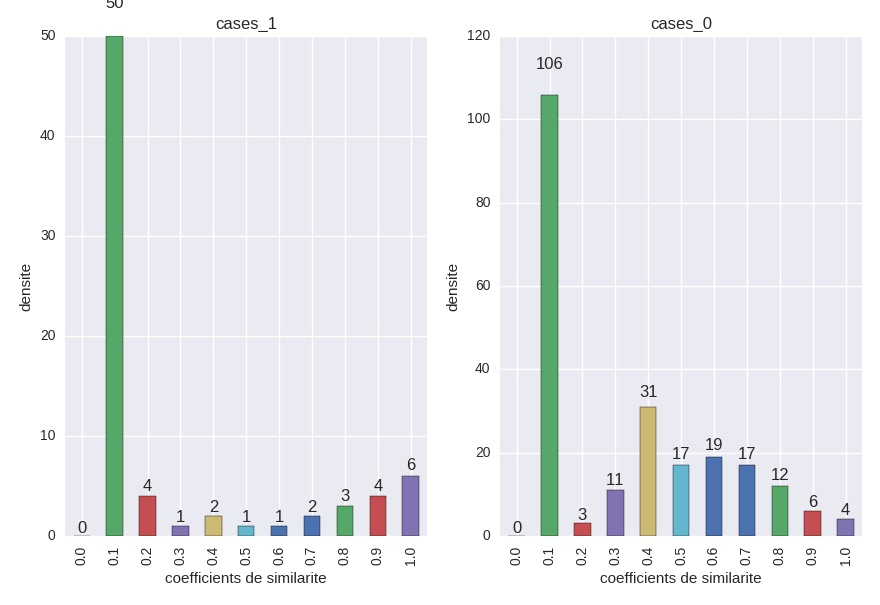
\includegraphics[scale = 0.55]{distribution_0_1_distance_pearson.jpeg}
\caption{Distribution des coefficients des similarit\'es selon les arcs qui sont incidents.
$cases\_1$ d\'esigne les arcs incidents et $cases\_0$ d\'esigne les arcs non incidents dans le {\em sous-r\'eseau de Champlan}.
Le coefficient de similarit\'e $0.1$ indique toutes les valeurs dans l'intervalle $[0.1, 0.2[$.
}
\label{distribution_0_1_distance_pearson}
\end{figure}
% ---- figure sous-reseau champlan.
% 4 erreur de similarite et categorisation de ces erreurs 
Nous disposons de la topologie \'electrique r\'eelle de {\em Champlan}.
Nous comparons  les coefficients de similarit\'e  calcul\'es par rapport aux arcs qui sont incidents dans la topologie de {\em Champlan}.
Pour ce faire, nous pr\'esentons, dans la figure \ref{distribution_0_1_distance_pearson}, les distributions des arcs incidents et non incidentes  en fonction des coefficients de similarit\'e. Les arcs non incidentes sont d\'esign\'es par $cases\_0$ et les arcs incidents par $cases\_1$.
	% arcs non adjacents : prkoi on a des coeff = 1?
		% ---- figure  profils_consommation_cases_0_similarite_1
		\begin{figure}[htb!] 
		\centering
		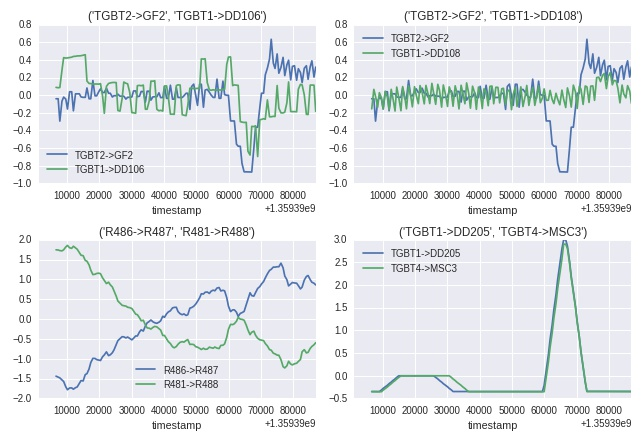
\includegraphics[scale = 0.65]{profils_consommation_cases_0_similarite_1.jpeg}
		\caption{ Profils de consommation des paires d'arcs n'ayant aucun \'equipement en commun. 
		En haut \`a gauche, nous avons les courbes des arcs $TGBT2->GF2$, $TGBT1->DD106$. 
		En haut \`a droite, les courbes des arcs $TGBT2->GF2$, $TGBT1->DD108$. 
		En bas \`a gauche, les courbes des arcs $R486->R487$, $R481->R488$.
		En bas \`a droite,  les courbes des arcs  $TGBT1->DD205$, $TGBT4->MSC3$
		}
		\label{profils_consommation_cases_0_similarite_1}
		\end{figure}
%		\FloatBarrier
		% ---- figure  profils_consommation_cases_0_similarite_1
	La distribution des arcs non incidents est asym\'etrique vers la gauche. Cela est normale puisque nous avons suppos\'e que les arcs non incidents ont des coefficients de similarit\'e qui tendent vers $0$. 
	Cependant, nous avons $4$ paires d'arcs qui ont des coefficients $corr(x->y,y->z) = 1$. La figure \ref{profils_consommation_cases_0_similarite_1} pr\'esente les profils de consommation de ces $4$ paires arcs. Nous constatons que :
	\begin{itemize}
		\item Les arcs $R486->R487$ et $R481->R488$ ont des profils oppos\'es et en appliquant la valeur absolue sur les valeurs de chaque s\'erie, les profils se superposent. Il n'y a aucune corr\'elation entre cette paire d'arcs. 
		\item Les arcs $TGBT1->DD205$ et $TGBT4->MSC3$ ont leurs profils qui se superposent et la corr\'elation de Pearson entre ces s\'eries est alors nulle.
		\item Les paires d'arcs $TGBT2->GF2$ et $TGBT1->DD106$ ont des courbes qui ont plusieurs points d'intersection. \`A ces points, le coefficient de similarit\'e est nul et est proche de $0$ au voisinage de ces points. La corr\'elation de Pearson entre ces s\'eries est alors nulle. 
	\end{itemize}
	Cela implique que le coefficient de similarit\'e est \'egal \`a $corr(x->y,y->z) = 1$ entre ces paires d'arcs $x->y,y->z$ par l'\'equation \ref{personDistance} alors que ces arcs n'ont aucun sommet en commun dans le graphe de la figure \ref{sousReseauChamplan}.
	Ces erreurs de corr\'elation sont introduites par la m\'ethode de calcul des coefficients.
	\newline  
	% arcs adjacents : prkoi on a des coeff = 0.1?
		% ---- figure profils_consommation_cases_1_similarite_0.1
		\begin{figure}[htb!] 
		\centering
		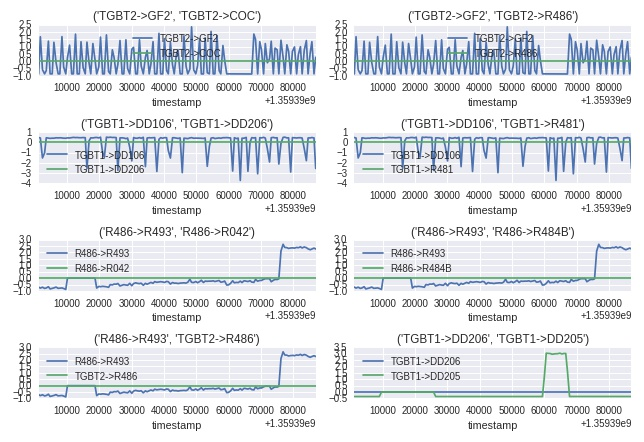
\includegraphics[scale = 0.65]{profils_consommation_cases_1_similarite_01.jpeg}
		\caption{ Profils de consommation des paires d'arcs ayant un \'equipement en commun. 
		les arcs $TGBT2->GF2$ et $TGBT2->COC$ partagent l'\'equipement $TGBT2$.}
		\label{profils_consommation_cases_1_similarite_01}
		\end{figure}
		% ---- figure  profils_consommation_cases_1_similarite_0.1
	En ce qui concerne la distribution des coefficients de similarit\'e des arcs incidents ($cases\_1$), elle est aussi asym\'etrique \`a gauche avec un pic  pour les coefficients appartenant \`a l'intervalle $[0.1,0.2[$. Pour comprendre cette distribution, nous repr\'esentons les profils de consommation de certaines paires d'arcs incidents  ayant leur coefficient de similarit\'e appartenant \`a  l'intervalle $[0.1,0.2[$ dans la figure \ref{profils_consommation_cases_1_similarite_01}.  
	Dans ces repr\'esentations, il y'a toujours une courbe constante et sa pr\'esence est due \`a l'impossibilit\'e de collecter des donn\'ees \`a cause d'une panne. 
	Cette s\'erie contient alors des valeurs nulles. Il y'a aussi la fourniture d'\'energie dans les branches. En effet, la source ne fournit que la quantit\'e d'\'energie demand\'ee par un \'equipement. Les s\'eries des arcs sont diff\'erentes et la distance de Pearson est la plus faible ($corr(x->y,y->z) = 0.1$). 
	Dans ce cas, les erreurs sont introduites par les donn\'ees et le fonctionnement du r\'eseau.
\newline	
Dans les cas d'erreurs de similarit\'e \'enonc\'ees plus haut, nous ne pouvons pas les \'eviter  pendant le calcul des coefficients parce que le m\'ecanisme de r\'ecup\'eration des donn\'ees est d\'efaillant et  l'arr\^et de la consommation d'\'electricit\'e d'une branche est masqu\'e par la mise en service de plusieurs serveurs dans une baie appartenant \`a une autre branche.
\newline 

% matrice de correlation et type d erreurs
Les coefficients de similarit\'e sont regroup\'es dans une matrice sym\'etrique  carr\'ee de dimension $N \times N$ avec $N$ le nombre d'arcs dans le {\em sous-r\'eseau de Champlan}.
Les lignes et les colonnes de la matrice sont les arcs du sous-r\'eseau. Chaque case de la matrice contient un coefficient de similarit\'e entre deux arcs. Les cases de la diagonale de la matrice contiennent les coefficients d'un arc avec lui-m\^eme et sont \'egales \`a $0$.  
Cette matrice est appel\'ee {\em matrice de corr\'elation} et se note $M_c$.
Sur cette matrice, diff\'erentes valeurs de seuils $s \in [0,1]$ sont test\'ees dans le but de d\'eterminer la matrice d'adjacence $M_{c,s}$ du {\em sous-r\'eseau de Champlan}. 
Des arcs $x->y$ et $x->z$ dont leur coefficient $corr(x->y, x->z) \ge s$ ont leur case $M_{c,s}[x->y, x->z] = 1$ sinon $M_{c,s}[x->y, x->z] = 0$ si $corr(x->y, x->z) < s$. 
La figure \ref{distrib_relationAdjacence_seuils_distancePerson} pr\'esente les distributions des relations d'incidences entre les arcs apr\`es l'application  des seuils sur la matrice de corr\'elation. Pour un seuil donn\'e, les relations d'incidences sont regroup\'ees en $4$ cat\'egories :
\begin{itemize}
	\item Les incidences {\em vrais positives} : il existe un sommet en commun entre les arcs et la case associ\'ee de la paire d'arcs $[x->y, x->z]$ est $M_{c,s}(x->y, x->z) = 1$. 
	\item Les incidences {\em vrais n\'egatives} : il existe aucun sommet en commun entre les arcs et la case associ\'ee de la paire d'arcs $[x->y, x->z]$ est $M_{c,s}(x->y, x->z) = 0$. 
	\item Les incidences {\em fausses positives} :  il existe aucun sommet en commun entre les arcs et la case associ\'ee de la paire d'arcs $[x->y, x->z]$ est $M_{c,s}(x->y, x->z) = 1$. 
	\item Les incidences {\em fausses n\'egatives} :  il existe un sommet en commun entre les arcs et la case associ\'ee de la paire d'arcs $[x->y, x->z]$ est $M_{c,s}(x->y, x->z) = 0$. 
\end{itemize}
Les incidences {\em fausses positives} et {\em fausses n\'egatives} constituent des {\em erreurs d'incidences} dans la matrice d'adjacence $M_{c,s}$. Nous consid\'erons aussi certaines incidences {\em vrai positives}  et {\em vrais n\'egatives} comme les {\em erreurs d'incidences}.
Chaque graphique affiche les erreurs d'incidences associ\'ees \`a un seuil. Par exemple, dans le graphique {\em VraiPositive\_ErreurAdjacence} de la figure \ref{distrib_relationAdjacence_seuils_distancePerson} nous avons $17$ paires d'arcs partageant un sommet pour un seuil $s=0.4$. De m\^eme, nous avons $57$ paires d'arcs n'ayant aucun sommet en commun pour un seuil $s=0.4$ dans le graphique {\em fauxNegatives\_ErreurAdjacence} de la figure \ref{distrib_relationAdjacence_seuils_distancePerson}. 
Nous observons qu'il n'existe aucun seuil qui 
maximise les nombres d'incidences {\em vrai positives}  et {\em vrai n\'egatives}  et qui
minimise les nombres  d'incidences {\em fausses positives} et {\em fausses n\'egatives}.
Et cela est due \`a l'introduction des erreurs des coefficients de similarit\'e dans la {\em matrice de corr\'elation} $matE$.
		% ---- figure distrib_relationAdjacence_seuils
		\begin{figure}[htb!] 
		\centering
		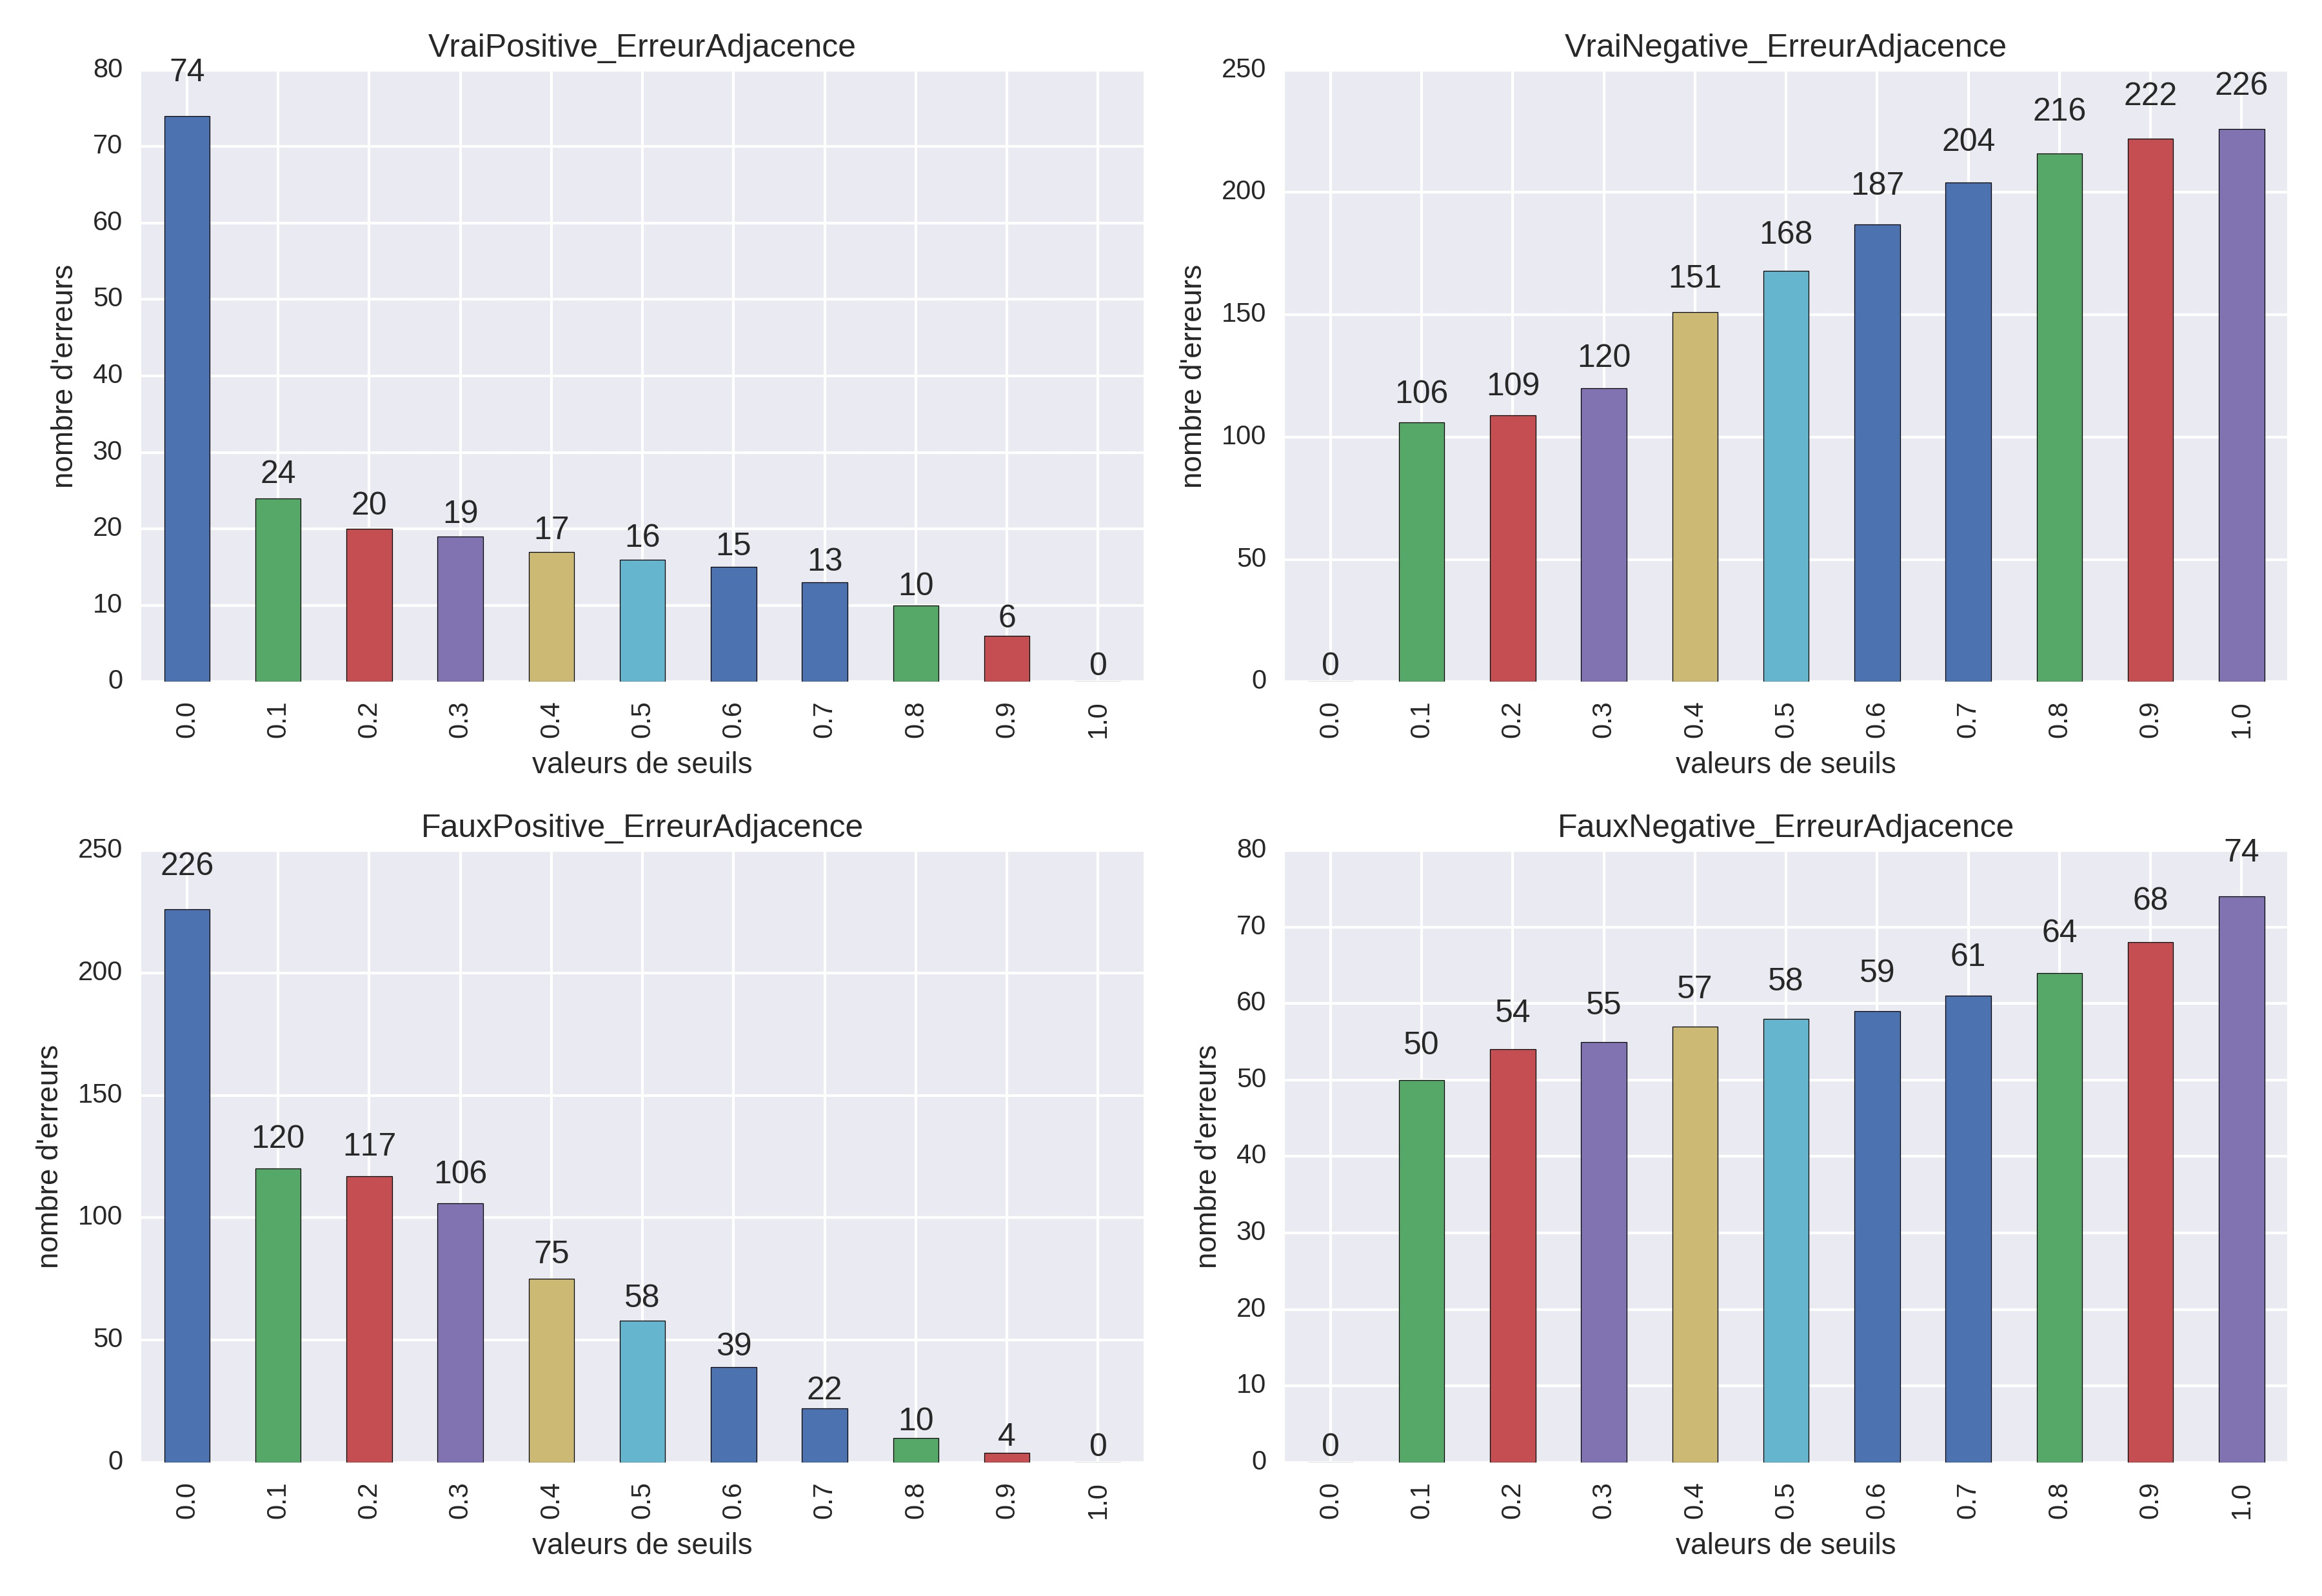
\includegraphics[scale = 0.14]{distrib_relationAdjacence_seuils.jpeg}
		\caption{ Distributions des relations d'incidences entre les arcs apr\`es l'application  de seuils. On distingue $4$ relations d'incidences entre les arcs : incidences {\em fausses positives} (graphique en bas \`a gauche),{\em fausses n\'egatives} (graphique en bas \`a droite), {\em vrais positives} (graphique en haut \`a gauche) et {\em vrai n\'egatives} (graphique en haut \`a droite).
		}
		\label{distrib_relationAdjacence_seuils_distancePerson}
		\end{figure}
		% ---- figure  distrib_relationAdjacence_seuils
\newline

% conclusion
%quel est la grandeur quon a selectionne
%travailler sur un sous graphe de champlan why 
%	presentation de champlan dans le chapitre precedent
%	description du reseau de champlan et presentation du reseau (affichage) 
% calcul des coefficient de similarite
%representation de la matrice de correlation
%comparer les faux positfs avec les faux negatifs 
%choix du seuil ou de epsilon
%conclusion
{\bf Conclusion} :
dans cette section, nous avons limit\'e notre \'etude sur un {\em sous-r\'eseau de Champlan} dans lequel les \'equipements ne sont pas aliment\'es par un onduleur. Ce choix fut pr\'ef\'er\'e \`a cause de notre hypoth\`ese qui stipule que les variations d'\'electricit\'e se propagent dans le r\'eseau. Nous avons calcul\'e les coefficients de similarit\'e $corr$ avec la grandeur {\em P} parce que c'est la seule grandeur qui fournit des mesures en monophas\'e et en triphas\'ee. Certains coefficients de similarit\'e sont \'erron\'es \`a cause des donn\'ees, de la m\'ethode de calcul  et du m\'ecanisme de fonctionnement du r\'eseau de Champlan. Ces coefficients forment la {\em matrice de corr\'elation} $M_c$ carr\'ee et sym\'etrique dans laquelle sont test\'es des seuils. 
Si $M_c$ ne contient aucune erreur de similarit\'e alors il existe un seuil qui d\'etermine la matrice d'adjacence de la topologie du sous-r\'eseau de Champlan. Malheureusement, nous ne sommes pas parvenus \`a d\'eterminer la bonne valeur de seuil et aussi \`a obtenir les coefficients de similarit\'e qui refl\`etent les relations d'adjacences des arcs.


\section{Conclusion du chapitre \ref{timeSeries}}
	Ce chapitre se subdivise en quatres parties.
La premi\`ere partie pr\'esente les domaines dans lesquels l'analyse des s\'eries temporelles est importante. Ensuite, nous exposons notre probl\`eme qui consiste \`a comparer deux s\'eries temporelles en supposant que les variations dans une s\'erie sont reproduites dans l'autre s\'erie.
Pour r\'esoudre notre probl\`eme, nous d\'ecidons de nous servir des m\'ethodes de classification de s\'eries temporelles.
Dans la seconde partie, nous d\'etaillons les m\'ethodes qui se regroupent en trois cat\'egories :
{\em similarit\'e sur les s\'eries enti\`eres, similarit\'e sur les parties significatives, similarit\'e par aggr\'egation des caract\'eristiques descriptives}. Chaque cat\'egorie d\'ecrit des distances de similarit\'e. 
Les avantages et les inconv\'enents de chaque cat\'egorie sont d\'ecrites dans la troisi\`eme partie. Ainsi, en analysant nos donn\'ees et en se basant sur notre hypoth\`ese, nous avons montr\'e que  les m\'ethodes sur les s\'eries enti\`eres sont adapt\'ees \`a notre probl\`eme.
En effet, notre hypoth\`ese stipule que deux arcs partageant un \'equipement ont les m\^emes profils de consommation et leur coefficient de similarit\'e est proche de $1$. Dans le cas contraire,  leur coefficient de similarit\'e tend vers $0$ et les profils de consommation ont des courbes diff\'erentes.
Nous avons alors choisi la {\em distance de Pearson} comme la m\'ethode de similarit\'e parce qu'elle est une m\'etrique, de complexit\'e lin\'eaire, ne traite pas le d\'ecalage temporel et enfin retourne des valeurs appartenant \`a l'intervalle $[0,1]$.
Nous avons appliqu\'e cette distance sur un {\em sous-r\'eseau du datacenter Champlan} parce que ce sous-r\'eseau ne poss\`ede aucun \'equipement aliment\'e par un onduleur.
Ensuite, la seule grandeur qui contient des valeurs en monophas\'e et triphas\'e est la grandeur $P$.
Les coefficients de similarit\'e entre les arcs obtenus avec la grandeur $P$ contiennent des erreurs de similarit\'e. Une erreur de similarit\'e est un coefficient proche de $1$ alors que les arcs ne concourent pas en un \'equipement et vice-versa.
Ces coefficients forment la {\em matrice de corr\'elation} qui appliqu\'ee \`a un seuil propose la matrice d'adjacence du sous-r\'eseau de champlan. Ceci est v\'erifi\'e \`a condition que les coefficients ne contiennent aucune erreur.
Enfin, nous avons montr\'e qu'il est difficile de d\'eterminer la bonne valeur de seuil en pr\'esence des coefficients de similarit\'e \'erron\'es.		


	
	%---- chapitre 3 : linegraphes
	\chapter{Line-graphes}
\label{linegraphesChapitre}
%--------------------------------------------------------------------
%------- formulation du probleme ---------------------
%--------------------------------------------------------------------
Dans le chapitre pr\'ec\'edent, nous avons d\'etermin\'e la matrice de corr\'elation $M_c$ du graphe $G$ d'un r\'eseau \'electrique. Cette matrice peut contenir des cases \'erron\'ees. Une case \'erron\'ee  $M_c[i,j]$ est un coefficient de corr\'elation proche de $1$ (resp. de $0$) entre les arcs $i$ et $j$ alors que ces arcs ne partagent aucune extr\'emit\'e (resp. ces arcs ont une extr\'emit\'e commune).
\newline
Nous consid\'erons une matrice $M$ de dimension identique \`a celle de $M_c$ telle que, pour toute valeur de seuil $s \in [0,1]$ et toute paire d'arcs $(i,j)$, $M[i,j] = 1$ si et seulement si $M_c[i,j] \ge s$. La matrice $M$ est la matrice d'adjacence d'un graphe non orient\'e $G_c$ dit {\em graphe de corr\'elation}. Cette matrice peut \'egalement contenir des cases \'erron\'ees.  
Une case \'erron\'ee $M[i,j] = 1$ d\'esigne la pr\'esence d'ar\^etes dans $G_c$ alors qu'il n'existe aucune ar\^ete entre les sommets $i$ et $j$ dans le line-grahe du graphe non-orient\'e sous-jacent au DAG $G$. 
De m\^eme, l'absence d'une ar\^ete entre $i$ et $j$ dans $G_c$ alors qu'elle est pr\'esente dans le line-grahe du graphe non-orient\'e sous-jacent \`a $G$ est aussi une case \'erron\'e  $M[i,j] = 0$.
\newline 
S'il n'existe aucune case \'erron\'ee dans la matrice $M$, alors $G_c$ est le line-graphe de graphe non-orient\'e sous-jacent au DAG $G$ et le line-graphe de $G$ est isomorphe \`a $G_c$.
Notre but est de d\'eduire le DAG $G$ \`a partir de $G_c$ en deux \'etapes :
\begin{itemize}
	\item D\'eterminer si $G_c$ est un line-graphe. Si c'est  le cas, d\'eduire le graphe dont $G_c$ est le line-graphe.
	\item Dans le cas o\`u $G_c$ n'est pas un line-graphe, proposer un algorithme qui modifie $G_c$ de telle sorte qu'il devient un line-graphe et ensuite d\'eduire le graphe dont le graphe $G_c$ modifi\'e est le line-graphe.
\end{itemize}
 Nous d\'esignons ce probl\`eme par {\em Proxi-Line}.
\newline
Nous allons, dans un premier temps, d\'ecrire les caract\'eristiques d'un line-graphe et le probl\`eme {\em Proxi-Line}. Ensuite nous pr\'esentons les algorithmes qui traitent ce probl\`eme et enfin nous expliquons la reconstruction de la topologie \`a partir du line-graphe d\'ecouvert par nos algorithmes. 





\section{Line-graphes : caract\'eristiques et propri\'et\'es}
	%------- introduction_line_graphes_caracteristiques ---------
	Dans la th\'eorie des graphes, un line-graphe est aussi appel\'e un {\em graphe adjoint} et ce terme est introduit par l'article de Harary et Norman \cite{harary1960some}.
Le line-graphe d'un graphe non orient\'e $G$ est un graphe qui repr\'esente la relation d'incidence entre les ar\^etes de $G$.
Nous allons d\'efinir formellement le line-graphe d'un graphe et pr\'esenter ses propri\'et\'es.

	
	%------- caracteristiques_linegraphes ----------------
	\subsection{Caract\'eristiques d'un line-graphe}
		
\begin{definition}
\label{definitionLineGraphe}
Soit $G = (V, E)$ un graphe non orient\'e.
\newline
Le line-graphe de $G$ est un graphe non-orient\'e $L(G) = (V',E')$ dans lequel 
$V'=E$ et 
une paire $[a,a']$ de sommets de $L(G)$ est une ar\^ete si et seulement si $a$ et $a'$ ont une extr\'emit\'e commune dans $G$.
\newline
Le graphe $G$ est appel\'e le {\em graphe racine} de $L(G)$.
\end{definition}

Si $G$ est un DAG alors  $L(G)$ est le line-graphe du graphe non-orient\'e sous-jacent \`a $G$.
\'Etant donn\'e que $G$ a $n$ sommets et $m$ arcs (sans arcs sym\'etriques), le graphe $L(G)$ a $m$ sommets et $|E'| = \sum_{i=1 }^{n} d_i(d_i -1)/2$ ar\^etes avec $d_i$ le degr\'e de chaque sommet $i$ de $G$.
\vspace{-0.3cm}

%% ---- figure GrapheRacineLineGrapheExemple
\begin{figure}[htb!]\vspace{-0.5em}
	\centering
	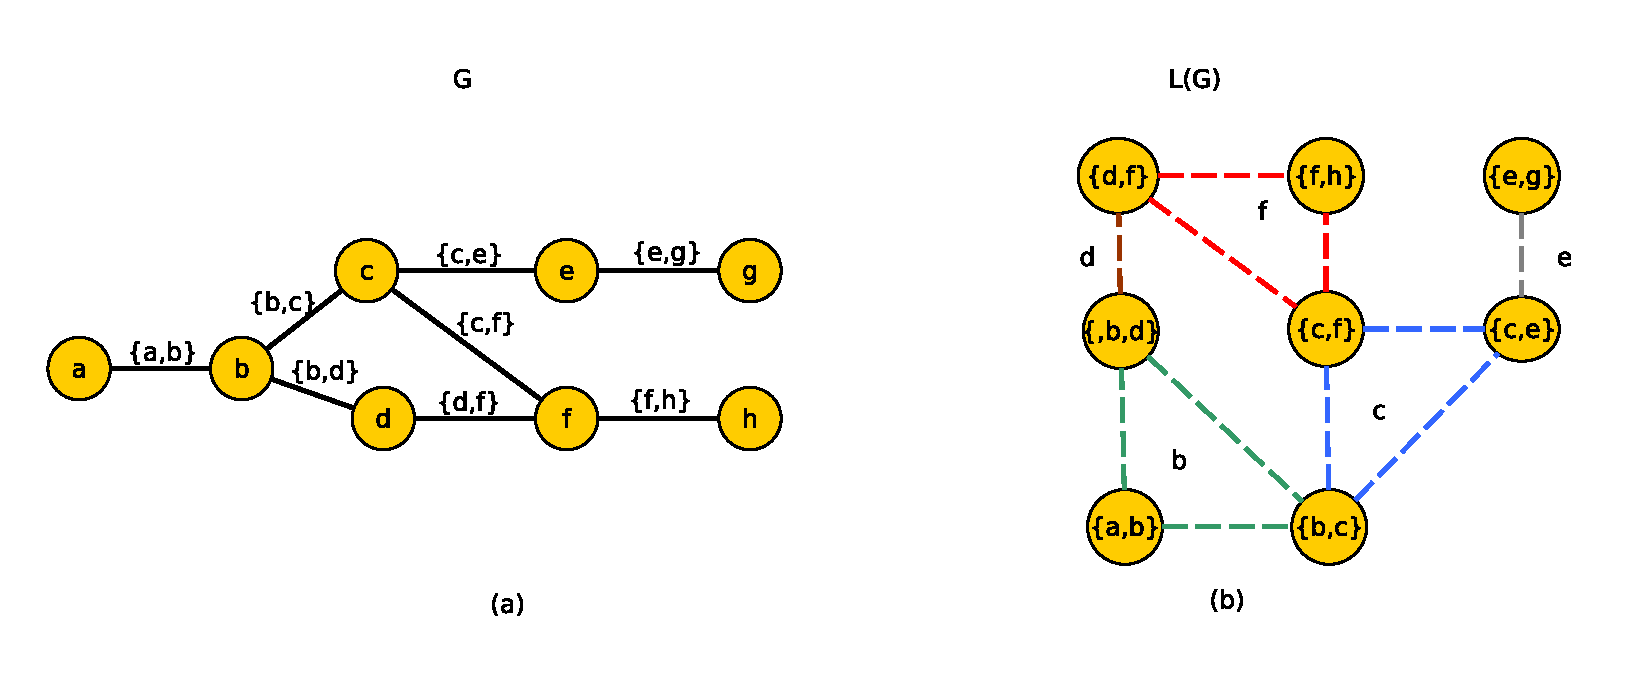
\includegraphics[scale=0.650]{grapheRacineLineGrapheExemple.eps}\vspace{-0.5em}
	\caption{ Le graphe $G$ et son line-graphe $L(G)$. 
			}\vspace{-0.5em}
	\label{grapheRacineLineGrapheExemple}
\end{figure}
%% ---- figure GrapheRacineLineGrapheExemple
\FloatBarrier
\vspace{0.3cm}

La figure \ref{grapheRacineLineGrapheExemple}(a) pr\'esente le graphe $G=(V,E)$ dans lequel l'ensemble $V$ contient $8$ sommets $V=\{a,b,c,d,e,f,g,h\}$ et l'ensemble $E$ contient $8$ ar\^etes \\ $E=\{ \{a,b\}, \{b,c\}, \{b,d\}, \{c,f\}, \{d,f\}, \{f,h\}, \{c,e\},\{e,g\} \}$. 
Chaque ar\^ete de $E$ devient un sommet de $L(G)$ dans la figure \ref{grapheRacineLineGrapheExemple}(b). Lorsque deux ar\^etes de $E$ ont une extr\'emit\'e  commune alors leurs sommets respectifs dans $L(G)$  sont adjacents.
Par exemple, dans la figure \ref{grapheRacineLineGrapheExemple}(b), les sommets $\{b,d\}$ et $\{d,f\}$ sont li\'es par une ar\^ete \`a cause du sommet $d \in V$. 
Nous construisons ainsi le graphe $L(G)$  qui contient $8$ sommets et $11$ ar\^etes.
Nous constatons qu'un sommet de $G$ correspond \`a une clique dans $L(G)$. 
En effet, les sommets de la clique $\{ \{a,b\},  \{b,c\},  \{b,d\} \}$ de taille $3$ dans $L(G)$ concourent \`a un point $b$ de degr\'e $3$ qui est un sommet de $G[V]$. Le sommet  $b$ de $G$  identifie la clique $\{ \{a,b\},  \{b,c\},  \{b,d\} \}$ dans $L(G)$.
Le graphe $L(G)$ est le  line-graphe de $G$ et $G$ est le {\em graphe racine}.
\newline

La notion de {\em line-graphe} a \'et\'e introduite par {\em Whitney} \cite{whitney1932congruent} en se basant sur la notion d'isomorphisme. Il montre que  si deux line-graphes sont isomorphes et connexes alors leurs graphes racines sont aussi isomorphes \`a l'exception des graphes triangle $K_3$ et \'etoile $K_{1,3}$. 
\begin{proposition} \cite{lineGraphe}
Le graphe \'etoile $K_{1,3}$ n'est pas un {\em line-graphe}.
\end{proposition}
\begin{Proof}
{\em
Supposons que $K_{1,3}$ est le line-graphe de $H$ ($K_{1,3} = L(H)$). 
Alors $H$ est un graphe connexe de quatre ar\^etes.
Tous les graphes connexes de quatres ar\^etes sont repr\'esent\'es dans la figure  \ref{graphesRacinesDeQuatresAretes}. 
Comme $L(C_4) = C_4$  et $L(K_{1,3} + e) = K_4 + e$ (voir figure \ref{graphesRacinesDeQuatresAretes}), $L(H)$ ne peut \^etre que l'un des trois arbres $P_4$, $K_{3,2}$ et $K_{1,4}$.
Ce qui est contraire \`a notre hypoth\`ese de d\'epart ($K_{1,3} = L(H)$).}
\end{Proof}
%\newline
% ------ figure graphes Racines De Quatres Aretes
\begin{figure}[htb!]\vspace{-0.5em}
	\centering
	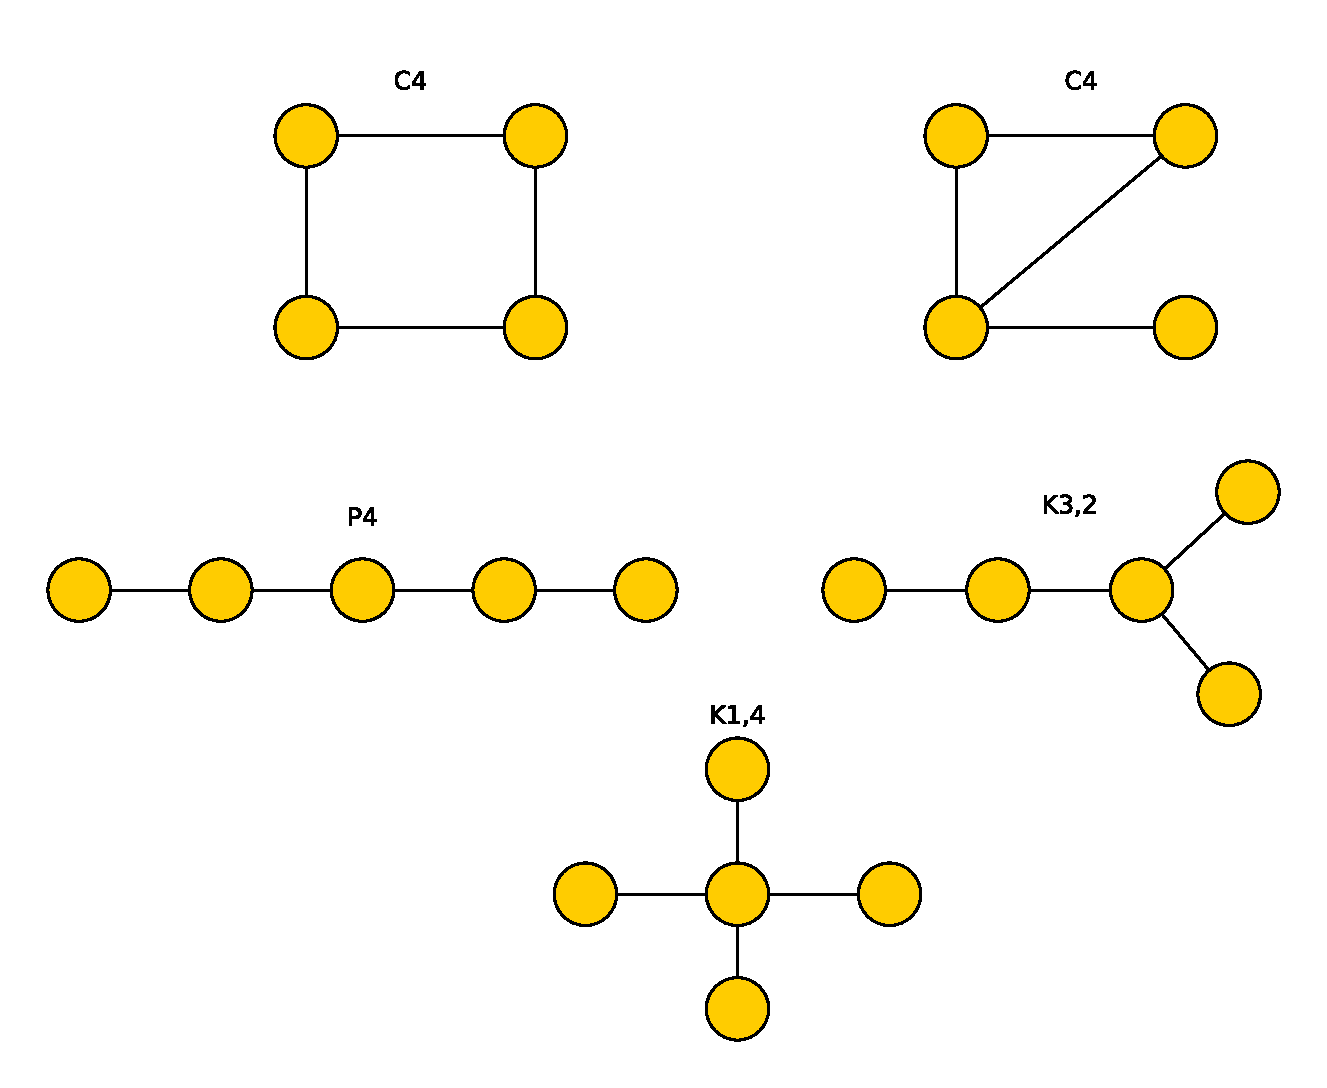
\includegraphics[scale=0.50]{graphesRacinesDeQuatresAretes.eps}\vspace{-0.5em}
	\caption{ Les graphes racines possibles de $K_{1,3}$ de quatres ar\^etes.}\vspace{-0.5em}
	\label{graphesRacinesDeQuatresAretes}
\end{figure}
% ------ figure graphes Racines De Quatres Aretes
\FloatBarrier
\vspace{0.3cm}

Le graphe \'etoile ($K_{1,3}$) a un r\^ole important dans la caract\'erisation des line-graphes.
La premi\`ere caract\'eristique provient des travaux de {\em Krausz} \cite{krausz1943demonstration} et elle est relative au partitionnement du line-graphe en sous-graphes. 
La seconde caract\'eristique, formul\'ee par {\em Van Rooij et Wilf} \cite{ROOIJetWILF1965interchange}, d\'ecrit la structure de base d'un graphe pour \^etre un line-graphe. 
Et enfin, la derni\`ere caract\'eristique pr\'esent\'ee par {\em Beineke\cite{beineke1968derived} et Hemminger} a d\'etermin\'e les neufs sous-graphes ne pouvant pas \^etre les sous-graphes induits  de line-graphes. 
\begin{theorem}\cite{lineGraphe}
\label{caracteristiquesLinegraphes}
Soit $H$ un graphe. Les affirmations suivantes sont \'equivalentes.
\begin{enumerate}[label = (\alph*)]
	\item $H$ est un line-graphe.
	\item Les ar\^etes de $H$ peuvent \^etre partitionn\'ees en sous-graphes complets appel\'es {\em cliques} tel qu'aucun sommet n'est contenu dans plus de deux sous-graphes. 
	\item $H$ ne contient pas $K_{1,3}$ comme sous-graphe et si deux triangles ont une ar\^ete commune alors le sous-graphe induit est $K_4$.
	\item Aucun des neufs sous-graphes de la figure \ref{neufSousGraphesInterditDesLineGraphes} ne peut \^etre un sous-graphe du line-graphe $H$.
\end{enumerate}
\end{theorem}

% ------ figure neuf Sous Graphes Interdit Des LineGraphes
\begin{figure}[htb!]\vspace{-0.5em}
	\centering
	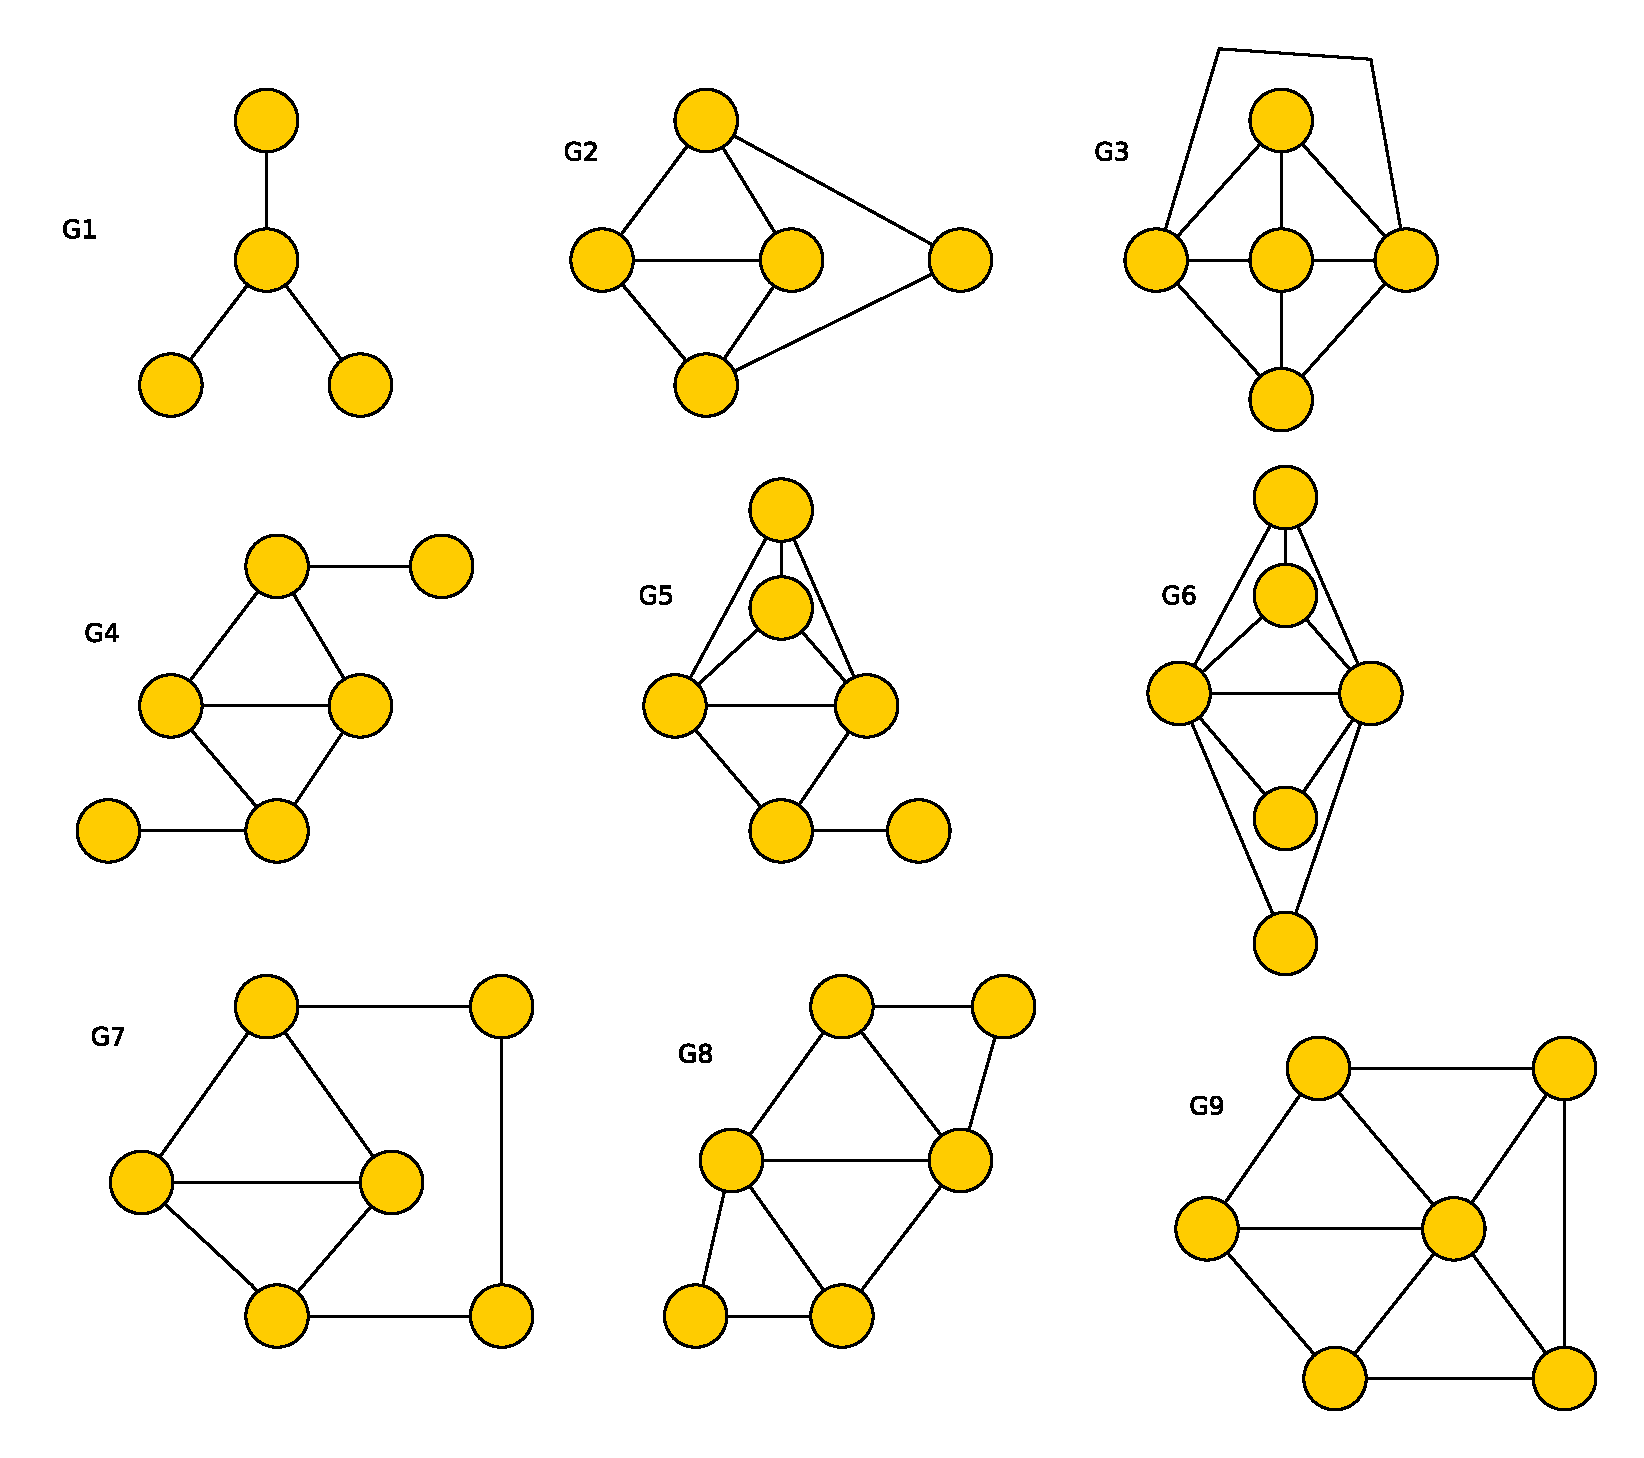
\includegraphics[scale=0.50]{neufSousGraphesInterditDesLineGraphes.eps}\vspace{-0.5em}
	\caption{ Les $9$ sous-graphes interdits dans un line-graphe. }\vspace{-0.5em}
	\label{neufSousGraphesInterditDesLineGraphes}
\end{figure}
% ------ figure neuf Sous Graphes Interdit Des LineGraphes
\FloatBarrier

{\bf Conclusion} :
soit $H$ un graphe et $G$ un graphe non-orient\'e.
Le graphe $H$ est un line-graphe de $G$ si le th\'eor\`eme \ref{caracteristiquesLinegraphes} est respect\'e.
Les graphes $H$ et $L(G)$ sont isomorphes et le graphe racine de $H$ est $L^{-1}(H)$.
Si $H$ est un line-graphe d'un graphe non orient\'e $G$,
alors le graphe $H$ admet un partitionnement en cliques et chaque clique correspond \`a un sommet de $G$. L'ensemble de cliques est appel\'e une {\em couverture de corr\'elation} et est not\'e ${\cal CC}(G)$.

	%------- proprietes_linegraphes -------------------------
	\subsection{Line-graphes ambigus}
		Soient $G$ un graphe non orient\'e et $H$ l'unique  line-graphe de $G$.
D'apr\`es le th\'eor\`eme \ref{caracteristiquesLinegraphes}(b), les ar\^etes de $H$ se partitionnent en cliques telles que chaque clique correspond \`a un sommet de $G$. 
\newline
Si le graphe de correction $G_c$ est sans erreur, alors il est un line-graphe et son partitionnement en cliques forme une {\em couverture de corr\'elation} not\'ee ${\cal CC}(G_c)$.
Existe-t-il plusieurs {\em couvertures de corr\'elation} de $G_c$ c'est-\`a-dire $G_c$ a-t-il plusieurs graphes racines qui sont isomorphes ?
Pour r\'epondre \`a cette question, nous d\'efinissons la notion d'{\em ambigu\"{i}t\'e}. 
\newline

\begin{definition}
Soient $G$ un graphe non orient\'e et $L(G)$ le line-graphe de $G$. 
\newline
Une ambigu\"{i}t\'e dans $L(G)$ est un sous-graphe isomorphe \`a l'un des graphes de la figure \ref{configurationAmbiguite}. Le sommet $X$ est appel\'e le {\bf point d'ambigu\"{i}t\'e}.
\end{definition}

Il a \'et\'e montr\'e que deux line-graphes isomorphes ont leurs graphes racine isomorphes \`a l'exception du graphe triangle \cite{whitney1932congruent}. Les graphes de la figure \ref{configurationAmbiguite} sont isomorphes mais leurs graphes racines ne sont pas isomorphes. Cela implique que leurs couvertures de corr\'elation sont diff\'erentes. D'o\`u la pr\'esence de sommets {\em ambigus}.

\begin{lemma}
	Soient $G = (V,E)$ un line-graphe  et $u$ un sommet de $G$. 
	\newline
	Si $G$ admet deux couvertures de corr\'elation, alors il existe au moins un sommet $u$ de $G$ tel que $G[\{u\} \cup \Gamma_{G}(u)]$ est une ambigu\"{i}t\'e dans laquelle $u$ est le point ambigu\"{i}t\'e.
\end{lemma}
	
\begin{Proof} 
{\em
	Consid\'erons deux couvertures de corr\'elation ${\cal CC}(G)$ et ${\cal CC'}(G)$ de $G$. 
	Il existe au moins un sommet $v \in V[G]$ qui n'est pas couvert par la (ou les) m\^eme(s) clique(s) dans  ${\cal CC}(G)$ et ${\cal CC'}(G)$.
	Soient deux cliques $c_1$ et $c_2$ (potentiellement vide) partitionnant $\{v\} \cup \Gamma_{G}(v)$ dans ${\cal CC}(G)$.
	Consid\'erons deux autres cliques $c_3$ et $c_4$ diff\'erentes de $c_1$ et $c_2$ partitionnant \'egalement $\{v\} \cup \Gamma_{G}(v)$ dans ${\cal CC}(G)$. 
	\newline
	Notons $c_{i,j}$ l'intersection de $c_{i}$ et $c_j$ pour tout $i \in \{1,2\}$ et $j \in \{3,4\}$. 
	Chaque sommet $w \in c_{i,j}$ est couvert par au plus deux cliques de $G$ dans ${\cal CC}(G)$, dont la clique $c_i$.
	Puisque $c_j$ est une clique alors ce sommet $w$ est voisin de tous les sommets de  $c_{i',j}$, pour $i' \ne i$.
	Les ar\^etes entre ces sommets sont dans $c'_i$, donc chaque ar\^ete $[w,z]$ pour tout sommet  $z \in c_{i',j}$ forme une clique dans le r\'eseau de flots.
	Ainsi, le cardinal de chaque ensemble  $c_{i,j}$ est \'egal \`a $1$.\newline
	Appelons $v_{i,j}$ le seul sommet pr\'esent dans $c_{i,j}$. 
	Il est possible d'avoir $v_{1,3} = v_{1,4}$ ou $v_{2,3} = v_{2,4}$.
	Si les deux \'egalit\'es sont v\'erifi\'ees, le sommet $v$ est alors couvert non pas par deux cliques mais par une seule de cardinalit\'e $3$.
	Ainsi, les seuls cas possibles sont alors r\'esum\'es par la figure  \ref{graphe2Couverture}.
	Le sommet $v$ est bien le point d'une ambigu\"{i}t\'e isomorphe \`a $G[\{u\} \cup \Gamma_{G}(u)]$.
} 
\hspace{16 em}$\qed$
\end{Proof}

Nous d\'eduisons le corollaire suivant :
\begin{corollary}
\label{corollaireGraphe2couverture}
Soit $G$ un line-graphe. 
\newline
Si $G$ admet deux couvertures de corr\'elation diff\'erentes, alors il est isomorphe \`a l'un des graphes de la figure  \ref{graphe2Couverture}.
\end{corollary}

% ----- figure configurationAmbiguite
\begin{figure}[htb!]\vspace{-0.5em}
	\centering
	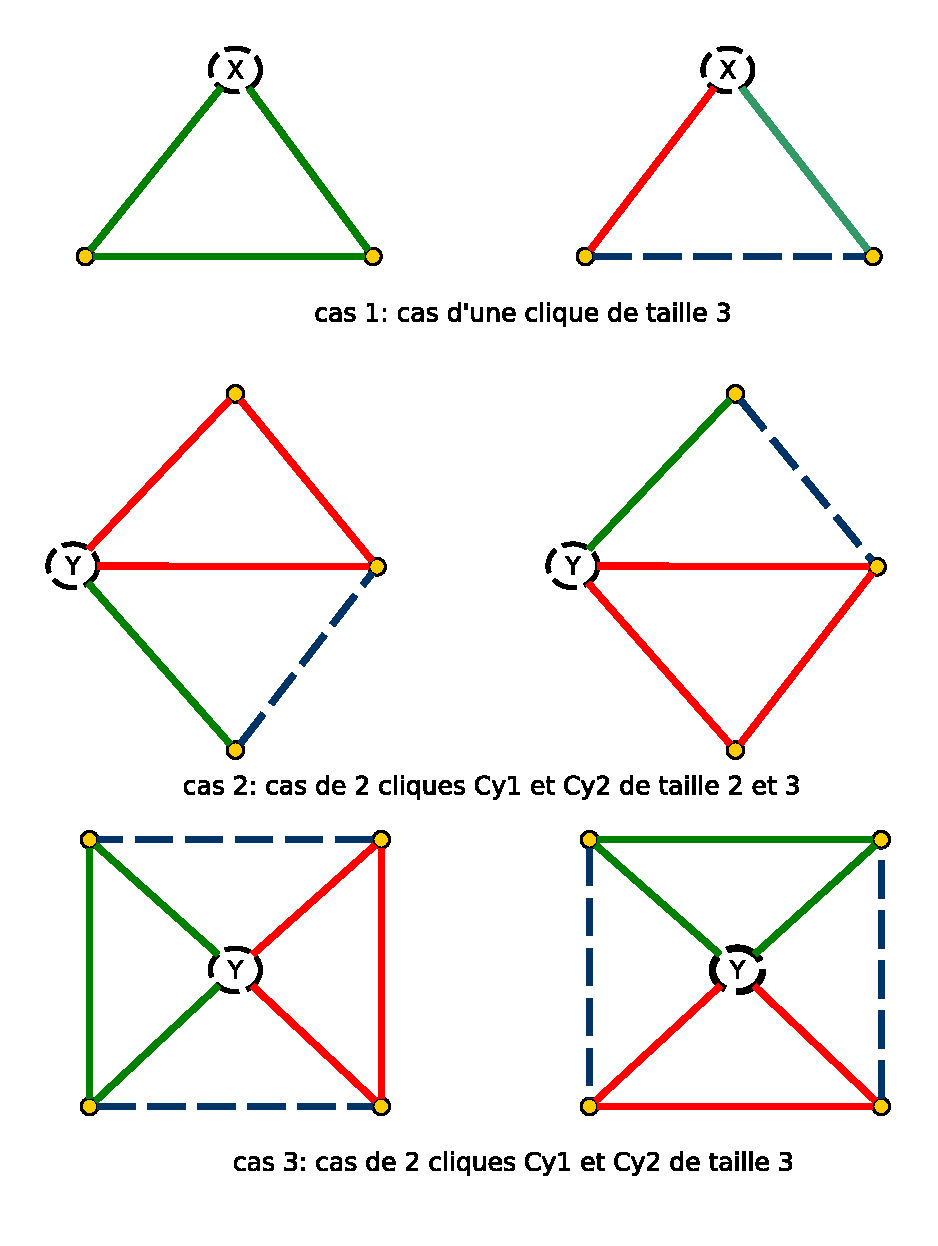
\includegraphics[scale=0.70]{configurationAmbiguite.eps}\vspace{-0.5em}
	\caption{ Configurations possibles d'une ambigu\"{i}t\'e au sommet X. }\vspace{-0.5em}
	\label{configurationAmbiguite}
\end{figure}
% ----- figure configurationAmbiguite
\FloatBarrier


En effet, si $G[\{u\} \cup \Gamma_{G}(u)]$ a une ambigu\"{i}t\'e, chaque ar\^ete, qui n'est pas li\'ee au point d'ambigu\"{i}t\'e, doit \^etre une ar\^ete d'une et une seule autre ambigu\"{i}t\'e de $G$. Et chaque sommet d'une ambigu\"{i}t\'e, qui n'est pas un point d'ambigu\"{i}t\'e, doit appartenir \`a une et une seule autre ambigu\"{i}t\'e de $G$ dont il n'est pas non  plus le point d'ambigu\"{i}t\'e.
De plus, chaque ar\^ete, n'\'etant pas couverte par les deux configurations de cliques possibles dans une ambigu\"{i}t\'e (les ar\^etes en pointill\'ees dans la figure \ref{configurationAmbiguite}), doit \^etre dans une autre ambigu\"{i}t\'e \`a laquelle elle appartient.
Ces contraintes font que si un graphe contient une ambigu\"{i}t\'e induite, alors il ne peut \^etre que dans un cas de la figure  \ref{graphe2Couverture}.

\begin{definition}
\label{cliquesCoherentes}
Soient $G$ un graphe, $u$ un sommet de $G$ et $\Gamma_G(u)$ les sommets voisins de $u$. 
\newline
Une partition de $\Gamma_G(u)$ en deux cliques $C_{u1}, C_{u2}$ est {\bf coh\'erente } si et seulement si chaque sommet $v$ de $C_{u1}$ (resp. $C_{u2}$) a au plus un voisin dans $C_{u2}$  (resp. $C_{u1}$).
\end{definition}

% ---- figure graphe de couverture
\begin{figure}[htb!] \vspace{-1.5em}
\centering
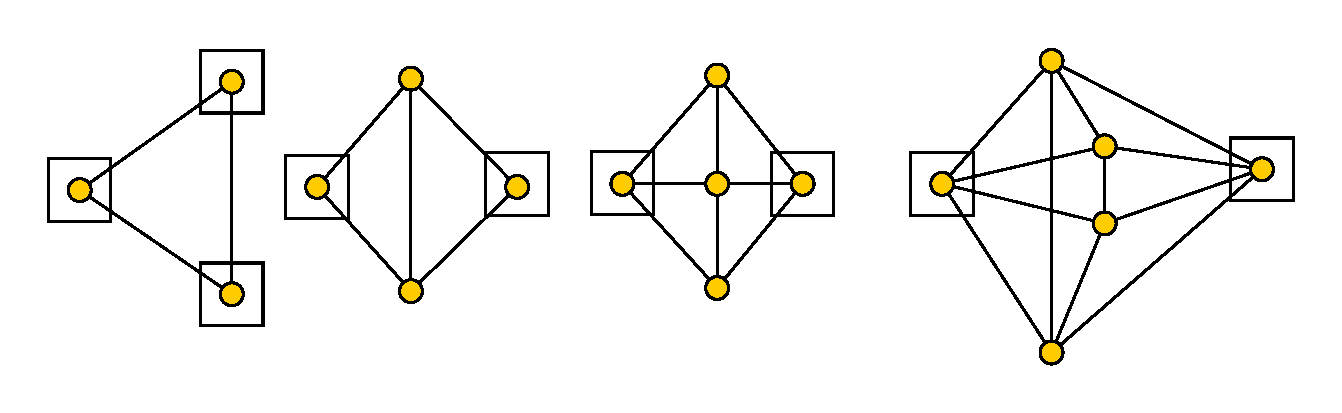
\includegraphics[scale=0.75]{graphe2Couverture.eps}
\caption{ Les graphes possibles de deux couvertures de corr\'elation avec les points d'ambigu\"{i}t\'es encadr\'es. }
\label{graphe2Couverture} 
\end{figure}
% ---- figure graphe de couverture
\FloatBarrier


{\bf Conclusion} : 
nous avons montr\'e que la {\em couverture de corr\'elation} d'un line-graphe est unique \`a l'exception des situations ambigu\"{i}t\'es. Les cas d'ambigu\"{i}t\'es sont pr\'esent\'es dans la figure \ref{graphe2Couverture}.





\section{Formulation du Probl\`eme {\em Proxi-Line}}

	%------- introduction_matrice_correlation ---------
	Soient $G$ un graphe non orient\'e d'un DAG,
 $G_c$ un graphe de corr\'elation de $G$ et 
 $M$ la matrice d'adjacence de $G_c$.
 \newline
 Notre probl\`eme est de d\'eterminer $G$ \`a partir de $G_c$. Pour ce faire, nous d\'ecidons de nous servir de la {\em couverture de corr\'elation}.
On a trois cas :
\begin{itemize}
	\item Soit $G_c$ est isomorphe \`a $L(G)$. Nous trouverons la couverture de corr\'elation unique qui donne $G$.
	\item Soit $G_c$ est un line-graphe non isomorphe \`a $L(G)$. 
		Modifier la matrice d'un line-graphe peut en effet le transformer en un autre line-graphe. Ce cas arrive rarement notamment lorsqu'il y a peu d'ar\^etes erron\'ees dans $G_c$. 
	\item Soit $G_c$ n'est pas un line-graphe. Dans ce cas, l'id\'ee est de corriger $G_c$ en ajoutant ou supprimant le minimum d'ar\^etes.
\end{itemize}
Nous resolvons le $3^{ieme}$ cas en introduisant le probl\`eme suivant :



	%------- probleme -----------------------------------------------
	\subsection{Probl\`eme}
		\'Etant donn\'e un graphe $G'$ qui a des ar\^etes en plus ou en moins par rapport \`a un autre graphe $G$ de m\^eme ensemble de sommets.
\begin{definition}
%La distance en $G$ et $G'$ est la distance de Hamming not\'ee $DH(G,G')$ entre leurs deux matrices d'adjacente, c'est-\`a-dire le nombre d'\'el\'ements ayant une valeur diff\'erente dans chacune des deux matrices.
Soient $G$ et $G'$ deux  graphes non orient\'es ayant le m\^eme ensemble de sommets.
\newline
La distance de Hamming entre les graphes $G$ et $G'$ not\'ee $DH(G,G')$ est le nombre d'ar\^etes pr\'esentes dans $G$ et pas $G'$ et inversement.
\end{definition}
Une distance de Hamming \'egale \`a $k$ $(k \in \mathbb{N})$ signifie qu'il existe $k$ cases diff\'erentes entre les matrices d'adjacence des graphes $G$ et $G'$.


\begin{definition}
Soit $G$ un graphe non orient\'e.
\newline
On appelle {\em distance line} de $G$, not\'ee $DL(G)$, la plus petite distance de Hamming entre $G$ et $G'$, un line-graphe ayant le m\^eme ensemble de sommets que $G$.
\end{definition}


Nous consid\'erons le probl\`eme suivant. \newline
{\bf Probl\`eme} Proxi-Line \newline
{\bf Donn\'ees} : Un graphe $G=(V,E)$, un entier $k$. \newline
{\bf Question} : $DL(G) \le k$ ? 
\newline


\begin{conjecture}
Proxi-Line est NP-complet.
\end{conjecture}

Ce probl\`eme g\'en\'eralise le probl\`eme {\em NP-complet} d\'efini et montr\'e  dans \cite{yannakakis1978node}, c'est-\`a-dire \'etant donn\'es un graphe $ G $ et un entier $k$, le probl\`eme de savoir s'il existe un line-graphe $ G'$ qui est un sous-graphe couvrant de $ G $ tel que $ dH (G, G' ) \leq k $ (c'est-\`a-dire, le probl\`eme Proxi-Line dans lequel seule la suppression d'ar\^etes  est autoris\'ee) utilise une solution de programmation lin\'eaire en nombres entiers   dans \cite{Halldorsson2013}. R\'ecemment, il a \'et\'e montr\'e au sein du laboratoire DAVID que l'op\'eration d'ajout d'ar\^etes uniquement dans le graphe de corr\'elation est aussi  {\em NP-complet}.


	%------- Conclusion description algorithmes -----------------------------------------------
%	\subsection{Conclusion de la formulation du probl\`eme}
%		
Nous avons consid\'er\'e que
la couverture de corr\'elation du graphe de corr\'elation $G_c$ est unique m\^eme en pr\'esence d'erreurs de corr\'elations et d'ambigu\"{i}t\'es.  La d\'etermination du graphe $G$ non orient\'e sous-jacent au DAG est ais\'ee.
\newline
Dans le cas o\`u la d\'etermination de couverture de corr\'elation de $G_c$ est impossible, nous avons d\'efini le probl\`eme {\em Proxi-Line}. Le but de {\em Proxi-Line} est de fournir le line-graphe de $G$ qui a le minimum d'ar\^etes diff\'erent par rapport $G_c$.  

%-----------------------------------------------------------------------------------------------------------
%------- algorithme de decouverte: couverture et correction ---------------------
%-----------------------------------------------------------------------------------------------------------
\section{Algorithmes de d\'ecouverte de topologie}

	
%%%%% ---- commentaire dominique pour l'intro
%Dire ce que cest le probleme tu regarde
%qu'est ce qui existe pour resoudre proxiline
%etant donn\'ee u graphe pour reconnaitre que cest un line graphe ou pas
%%%%% ---- commentaire dominique pour l'intro

Le probl\`eme consid\'er\'e ici est, 
\'etant donn\'e un graphe, de d\'eterminer s'il est un line-graphe et dans ce cas donner le graphe racine.
Nous d\'ebutons par l'\'etat de l'art des algorithmes de couverture en cliques puis pr\'esentons nos algorithmes tout en sp\'ecifiant leurs particularit\'es par rapport aux m\'ethodes existantes. 

\subsection{Recherche de Couverture en cliques}
Diff\'erents travaux ont \'et\'e r\'ealis\'es sur la d\'ecouverte de {\em couverture en cliques} dans les line-graphes.
Parmi lesquelles, nous citons  l'algorithme de {\em Roussopoulos}  \cite{ROUSSOPOULOS1973108} qui utilise une propri\'et\'e des line-graphes provenant des travaux de {\em Krausz} \cite{krausz1943demonstration}. 
Il affirme que le graphe $G$ est un line-graphe si ses ar\^etes  peuvent \^etre partitionn\'ees en cliques  de telle sorte qu'aucun sommet ne soit couvert par plus de deux cliques. 
L'algorithme propos\'e d\'etecte si $G$ est un line-graphe et il fournit, en plus, son graphe racine en temps lin\'eaire $O(max(\{m,n\}))$, avec $n$ et $m$ les nombres respectifs de sommets et d'ar\^etes.
\newline
Un autre algorithme, propos\'e par {\em Klauss Simon} et {\em Daniele Degiorgi} \cite{decompositionEnCliques}, est une simplication du probl\`eme de reconnaissance de line-graphes. Bas\'e sur la preuve de {\em Oystein Ore} du th\'eor\`eme de {\em Whitney} \cite{whitney1932congruent}, il stipule que deux line-graphes connexes avec plus de quatre sommets sont isomorphes si et seulement si leurs graphes racines sont aussi isomorphes et que ces graphes  doivent \^etre diff\'erents de $K_{1,3}$ et $K_3$. Il d\'etermine en un temps lin\'eaire une couverture \'etant mise \`a jour sommet apr\`es sommet. 
L'inconv\'enient de cette m\'ethode est le traitement de sommets appartenant \`a des cliques ayant d\'ej\`a \'et\'e d\'ecouverts parce qu'il applique le partitionnement sur la liste des sommets obtenus.
\newline
L'algorithme de {\em Philippe Lehot} \cite{decompositionEnCliquesParArcs} a une complexit\'e en $O(n) + m$ avec $n$ le nombre de sommets de $G$ et $m$ le nombre d'ar\^etes de $L(G)$.
Il recherche les $9$ sous-graphes de la figure \ref{neufSousGraphesInterditDesLineGraphes} et il utilise le th\'eor\`eme de {\em Van Rooij et Wilf} \cite{ROOIJetWILF1965interchange} qui \'enonce qu'un graphe $G$ est un line-graphe si $G$ ne contient pas de sous-graphe induit $K_{1,3}$ et si deux graphes triangles  {\em impairs} ont une ar\^ete commune, alors le sous-graphe induit par ces sommets est une clique $K_4$. 
Rappelons qu'un graphe triangle (c'est-\`a-dire un cycle de longueur $3$) $\{a_1,a_2,a_3\} \subseteq V(L(G))$ est {\em impair} s'il existe un sommet $e \in V(G)$ adjacent \`a  au moins un des sommets $\{a_1, a_2, a_3\}$. Ce triangle est {\em pair} si chaque sommet de ce triangle est adjacent \`a $0$ ou $2$ autres sommets. Cet algorithme est d\'etaill\'e dans la section \ref{algoCouverture}.
%% graphe odd = impair/ even=pair
%A triangle in a graph is even if every other node is adjacent to 0 or 2 nodes in the triangle; it is odd otherwise. 
%%
\newline
Tous les algorithmes existants ne retournent  aucun r\'esultat lorsque le graphe  de corr\'elation $G_c$ poss\`ede des cases erron\'ees c'est-\`a-dire qu'il n'est pas un line-graphe. 
Cependant, la m\'ethode propos\'ee par {\em Halld{\'o}rsson and al.} \cite{Halldorsson2013} 
utilise un algorithme g\'en\'etique pour corriger un graphe de corr\'elation pour en obtenir un line-graphe. 
En effet, il propose une m\'ethode de d\'ecouverte de la g\'en\'ealogie de population en se basant sur les haplotypes partag\'es dans les g\'enomes des individus.  
Un haplotype est un groupe d'all\`eles dans un organisme qui est transmis ensemble par un parent.
Il mod\'elise un graphe dit {\em Clark Consistency} \cite{halldorsson2011clark} dans lequel les ar\^etes sont les haplotypes (ils sont uniques dans les g\'enomes) et les sommets sont les individus.
Cette m\'ethode recherche le graphe racine induit par le graphe {\em Clark Consistency} si celui ci est un line-graphe. Dans le cas o\`u le graphe {\em Clark Consistency graph} n'est pas un line-graphe, l'algorithme suppose qu'il existe des sommets en plus dans le {\em graphe Clark Consistency}, va les supprimer afin que le graphe devienne un line-graphe et enfin retourner le graphe racine.     
Le graphe {\em Clark consistency (CC)} a \'et\'e propos\'e dans  la m\'ethode d'identification d'haplotypes par {\em Andrew Clark}. 
En effet, {\em Andrew Clark} consid\`ere un ensemble de g\'enomes d'individus qui ont des haplotypes homozygotes et h\'et\'erozygotes. Il suppose que deux g\'enomes n'ont pas les m\^emes paires d'haplotypes. Les sommets du graphe CC sont les g\'enomes des individus et une ar\^ete de graphe CC entre deux g\'enomes existe s'ils partagent le m\^eme haplotype (homozygote ou h\'et\'erozygote). Les ar\^etes de ce graphe sont form\'ees par des individus partageant les m\^emes haplotypes. 
%%%
%A key component of our approach is the graph of potential sharing of haplotypes between individuals. This graph, called the Clark consistency (CC) graph, was first suggested in the context of a method for haplotype phasing by Andrew Clark [10]. Given the genotypes of a set of individuals, the CC graph has one node for each individual and an edge between two individuals if their genotypes are consistent with sharing a haplotype, i.e., if for every site where one of the individuals is homozygous, the other individual is either homozygous for the same allele or heterozygous. As the haplotypes of individuals that are homozygous for the whole region being considered are easily determined, we assume that every given individual has two different haplotypes (i.e., it is heterozygous for at least one of the genotyped markers) and no two individuals have the same pair of haplotypes.
%%%
Le probl\`eme de d\'ecouverte de line-graphes \'etant {\em NP-Complet}, la solution propos\'ee r\'ealise un algorithme de suppression de sommets et d'ar\^etes. 
L'algorithme de suppression de sommets est une 6-approximation alors que celui des ar\^etes est de complexit\'e $O(n*m)$ avec $m$ le nombre de sommets et $n$ le nombre d'ar\^etes.
Dans le cas o\`u des suppressions sont effectu\'ees, le line-graphe fourni est le plus proche possible du line-graphe de l'arbre g\'en\'ealogique.
La particularit\'e de la solution est l'absence d'ar\^etes ajout\'ees dans le line-graphe et cela implique que cette solution est inapplicable dans notre probl\`eme o\`u il existe des ar\^etes inconnues dans notre graphe de corr\'elation. En plus, l'ensemble de nos sommets dans le graphe de corr\'elation est connu contrairement \`a l'algorithme de {\em Halld{\'o}rsson et al.} qui suppose que les sommets doivent \^etre supprim\'es pour atteindre un line-graphe.
\newline
Nous nous basons sur l'algorithme de {\em Lehot} parce qu'il s'ex\'ecute en un temps lin\'eaire en effectuant un traitement sommet par sommet pour la reconnaissance de sous-graphes complets. Ce traitement permet de s\'electionner les cliques existantes et les sommets, n'appartenant \`a aucune clique, qui n\'ecessitent une modification de leur voisinage.
	
	%------- algo couverture -----------------------------------------------
	\subsection{Algorithme de couverture}
		\label{algoCouverture}
		% description de l'algo de lehot
L'algorithme de {\em couverture} que nous proposons est une am\'elioration de celui de {\em Lehot}.
Ainsi, nous pr\'esentons tout d'abord bri\`evement le principe de l'algorithme de couverture en cliques de {\em Lehot} \cite{decompositionEnCliquesParArcs}. 
\newline
Soient $H$ et $G$ deux graphes. Nous supposons que $H$ est le line-graphe de $G$ ($H=L(G)$).
Le but de cet algorithme est d'identifier le graphe racine $L^{-1}(H)$ de $H$.
L'algorithme va construire $G$  au fur et \`a mesure en identifiant les cliques dans $H$. 
Les ar\^etes et les sommets de $H$ et $G$ peuvent avoir au cours de l'ex\'ecution plusieurs \'etats :
%''----------- sommets de H et G 
\begin{itemize}
	\item Sommet ``bien-d\'efini'' : un sommet d\'ecouvert de $G$ tel que la clique correspondante dans $H$ a \'et\'e trouv\'ee et identifi\'ee.
	\item Sommet ``\`a moiti\'e-nomm\'e'' :  un sommet de $H$ tel que  l'ar\^ete correspondante dans $G$ a une extr\'emit\'e  ``bien-d\'efinie''. 
	\item Sommet ``pleinement-nomm\'e'' : un sommet de $H$ tel que l'ar\^ete correspondante dans $G$  a des extr\'emit\'es ``bien-d\'efinies''.
	\item Sommet ``basique'' : un sommet de $H$ est une ar\^ete de $G$. Ces sommets sont not\'es $x-y$ dans $H$ avec $x$ et $y$ des sommets d\'ecouverts de $G$.
	\item Sommet ``partag\'e'' : sommet de $H$ partageant une ar\^ete avec des sommets ``basiques'' adjacents. Ce sommet est une extr\'emit\'e commune entre des ar\^etes de $G$ incidentes. 
\end{itemize}
%''----------- sommets de H et G 


L'id\'ee de cet algorithme est de d\'eterminer une couverture de corr\'elation de $H$ en d\'etectant, selon $3$ cas \cite{decompositionEnCliquesParArcs} dans $H$, 
les sommets partag\'es adjacents \`a un sommet ``basique'' qui forment une clique.
Nous illustrons le fonctionnement de l'algorithme avec l'exemple suivant illustr\'e par la figure \ref{deroulementAlgorithmeLehotRechercheSommetsPartages}.
L'algorithme s\'electionne deux sommets ``basiques''  $1-2, 2-3$ et  l'ensemble $X$ des sommets adjacents aux sommets ``basiques''.
Si $X = \emptyset$ alors il n'existe pas de sommet partag\'e dans  $G$ et les sommets $1-2, 2-3$ sont \'etiquet\'es ``\`a moiti\'e nomm\'e'' (figure \ref{deroulementAlgorithmeLehotRechercheSommetsPartages}(a)).
Si $X=\{x\}$ alors le sommet $x$ est un sommet partag\'e dans  $H$ si $x = 2-4$ car le triangle $\{x, 1-2, 2-3\}$ est impair. Dans le cas o\`u $x = 1-3$, le  triangle $\{x, 1-2, 2-3\}$ est pair et
aucun sommet d\'ecouvert dans $G$ n'est incident aux sommets du triangle $\{x, 1-2, 2-3\}$ (figure \ref{deroulementAlgorithmeLehotRechercheSommetsPartages}(b)). 
Le sommet $x$ dans $H$ est \'etiquet\'e ``pleinement-nomm\'e'' et les autres sommets $1-2, 2-3$ dans $H$ sont \'etiquet\'es ``\`a moiti\'e nomm\'es''.
Si $X=\{x,y\}$, il n'existe  aucun sommet partag\'e dans  $H$ si $x$ et $y$ sont adjacents dans $H$. Dans le cas o\`u  ils ne sont pas adjacents alors ils forment deux triangles avec $1-2, 2-3$. Si $x=2-4$ et $y=1-3$ alors le triangle $\{2-4,1-2, 2-3\}$ est impair et $x$ est le sommet partag\'e dans $H$
(figure \ref{deroulementAlgorithmeLehotRechercheSommetsPartages}(c)).
Enfin pour $|X| = |\{a,b,c, \cdots\}| = 3$, le sommet $b$ dans $H$ est \'etiquet\'e sommet partag\'e si $a$ est adjacent \`a $b$ sinon le sommet $a$ devient le sommet partag\'e.
La derni\`ere \'etape s\'electionne al\'eatoirement un sommet ``\`a moiti\'e-nomm\'e'' dans $H$ qui est adjacent \`a un sommet  ``pleinement-nomm\'e'' dans $H$. Si ce sommet n'est pas d\'ej\`a couvert par une clique alors il est ``pleinement-nomm\'e'' et il est un sommet partag\'e dans $H$. 
\`A la fin de cette \'etape, tous les sommets sont \'etiquet\'es \`a ``pleinement-nomm\'e"  dans $H$ et ils deviennent des sommets partag\'es dans $H$.
\newline
L'algorithme s'ex\'ecute  en $O(m)+m'$ avec $m$  le nombre d'ar\^etes dans $G$ et $m'$ le nombre d'ar\^etes dans $L(G)$. Il retourne la liste de cliques d\'ecouvertes dans $H$ dans laquelle chaque clique correspond  \`a un sommet de $G$. Cette liste de cliques est appel\'ee {\em couverture de corr\'elation} (${\cal CC}$).
Malheureusement, si $H$ n'est pas un line-graphe alors il ne retourne pas de couverture partielle.

\subsubsection{Description de l'algorithme de couverture}
Nous proposons  l'algorithme de {\em couverture} (voir algorithme \ref{algo:couverture}) en lien avec celui de {\em Lehot} qui couvre  autant que possible les sommets du graphe de corr\'elation  $G_c$ par une ou deux cliques.
Notre algorithme retourne la {\em couverture de corr\'elation} (${\cal CC}$) de $G_c$ si la matrice d'adjacence de $G_c$ ne contient aucune case erron\'ee sinon il renvoie une {\em couverture de corr\'elation partielle} de $G_c$.
\newline
%% ---- figure etapes de decouverte de l'algo de lehot
\begin{figure}[htb!]
	\centering
	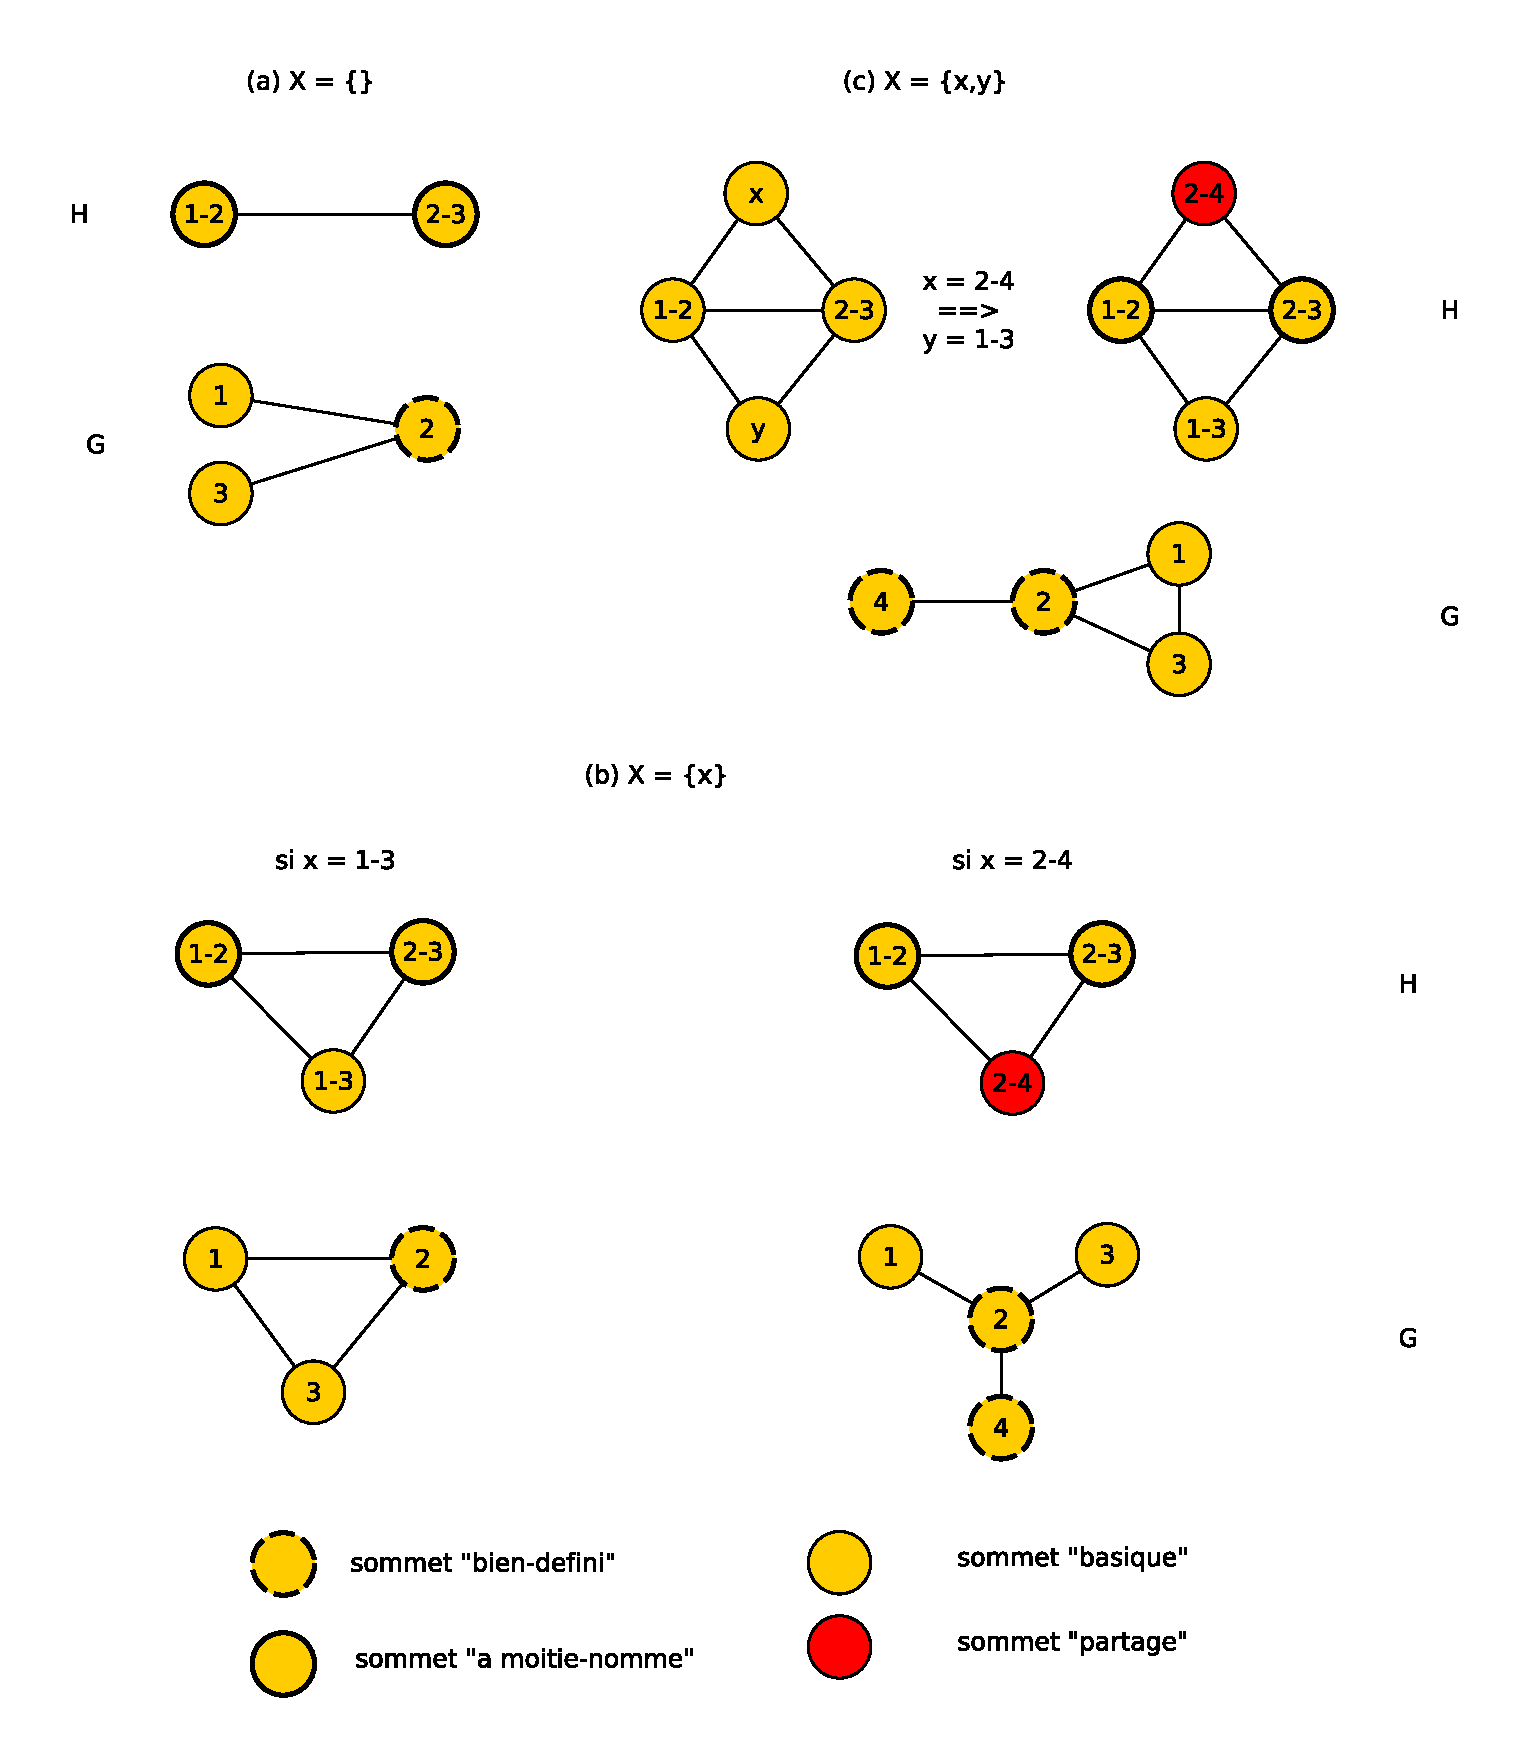
\includegraphics[scale=0.50]{deroulementAlgorithmeLehot.eps}\vspace{-0.5em}
	\caption{ Identification des sommets partag\'es dans le graphe $H$ et nommage des sommets de $G$. }\vspace{-0.5em}
	\label{deroulementAlgorithmeLehotRechercheSommetsPartages}
\end{figure}
%% ---- figure etapes de decouverte de l'algo de lehot
\FloatBarrier

Soient $G_c = (V,E)$ un graphe de corr\'elation et $Cliq(v)$ l'\'etat de chaque sommet $v$ de   $G_c$.
L'algorithme de {\em couverture} va construire une couverture de corr\'elation ${\cal CC}(G_c)$ de $G_c$ en ajoutant des cliques d\'ecouvertes dans ${\cal CC}(G_c)$.  
Une clique est un ensemble de sommets qui induit un sous-graphe complet. 
Si un sommet appartient \`a une clique alors il est couvert par cette clique. 
De m\^eme, si deux sommets $u$ et $v$ appartiennent \`a une m\^eme clique, alors la clique couvre l'ar\^ete $[x,y]$.
Initialement ${\cal CC}(G_c)$ est vide et chaque sommet de $v \in V$ a un \'etat $Cliq(v)=0$. 
\newline
\`A chaque \'etape de l'algorithme, chaque sommet $v$ a $5$ \'etats possibles :
\begin{itemize}
	\item $Cliq(v)=0$ : le sommet $v$ n'est couvert par aucune clique. Il correspond \`a un sommet ``basique'' dans l'algorithme de {\em Lehot}.
	\item $Cliq(v)=1$ : le sommet $v$ est couvert par une clique ou deux cliques. Dans le cas o\`u il est couvert par deux cliques, l'intersection de ces cliques donne le sommet $v$. Ce sommet est \'etiquet\'e ``pleinement-nomm\'e" dans l'algorithme de {\em Lehot}.
	\item $Cliq(v) = 2$ : le sommet $v$ est couvert par une clique et peut \^etre couvert par une seconde clique. Ce sommet est ``bien-nomm\'e" dans l'algorithme de {\em Lehot}.
	\item $Cliq(v) = 3$ : le sommet $v$ est un sommet ambigu. L'algorithme doit identifier la clique \`a laquelle il appartient pour qu'elle devienne un sommet partag\'e dans l'algorithme de {\em Lehot}.
	\item $Cliq(v) = -1$ :  le sommet $v$ est couvert par plus de deux cliques. Il est contenu dans l'ensemble $\cal C$ et doit \^etre corrig\'e par l'algorithme de correction.
\end{itemize}

Nous choisissons un sommet $v$ de degr\'e minimum qui n'appartient \`a aucune clique ou qui est un sommet ambigu. 
S'il existe une partition coh\'erente (voir d\'efinition \ref{cliquesCoherentes}) de ce sommet et de son voisinage $\{v\} \cup \Gamma_{G_c}(v)$ en deux cliques $C_1, C_2$, alors ces deux cliques sont contenues dans la couverture de corr\'elation ${\cal CC}(G_c)$ en cours de construction. Les sommets $v$ et $u$ (avec $u \in  \Gamma_{G_c}(v)$), appartenant \`a $C_1$ ou $C_2$, ont leur \'etat modifi\'e \`a chaque \'etape de l'algorithme de la mani\`ere suivante :
\begin{itemize}
\item $Cliq(v) = 1$ si son \'etat pr\'ec\'edent est \'egal \`a $0$ et la clique $C_2$ est vide. 
\item $Cliq(v) = 3$ si son \'etat pr\'ec\'edent est \'egal \`a $0$ et la clique $C_2$ est non vide. 
\item $Cliq(v) = 2$ si son \'etat pr\'ec\'edent est diff\'erent de $0$.
\item $Cliq(u) = 1$ si son \'etat pr\'ec\'edent est \'egal \`a $0$ et l'ensemble des ar\^etes incidentes \`a $u$ est vide.
\item $Cliq(u) = 2$ si son \'etat pr\'ec\'edent est \'egal \`a $3$ et l'ensemble des ar\^etes incidentes \`a $u$ est vide.
\item $Cliq(u) = 3$ si son \'etat pr\'ec\'edent est \'egal \`a $0$ et l'ensemble des ar\^etes incidentes \`a $u$ est non vide.
\item $Cliq(u) = -1$ si son \'etat pr\'ec\'edent est \'egal \`a $3$ et l'ensemble des ar\^etes incidentes \`a $u$ est non vide.
\end{itemize} 
Dans le cas o\`u il n'existe aucune partition coh\'erente (voir d\'efinition \ref{cliquesCoherentes}) au sommet $v$, son \'etat est \`a $Cliq(v)=-1$.
\newline
%\vspace{-1.5cm}
  %% ---- figure etapes de decouverte de l'algo de lehot
\begin{figure}[htb!]
	\centering
	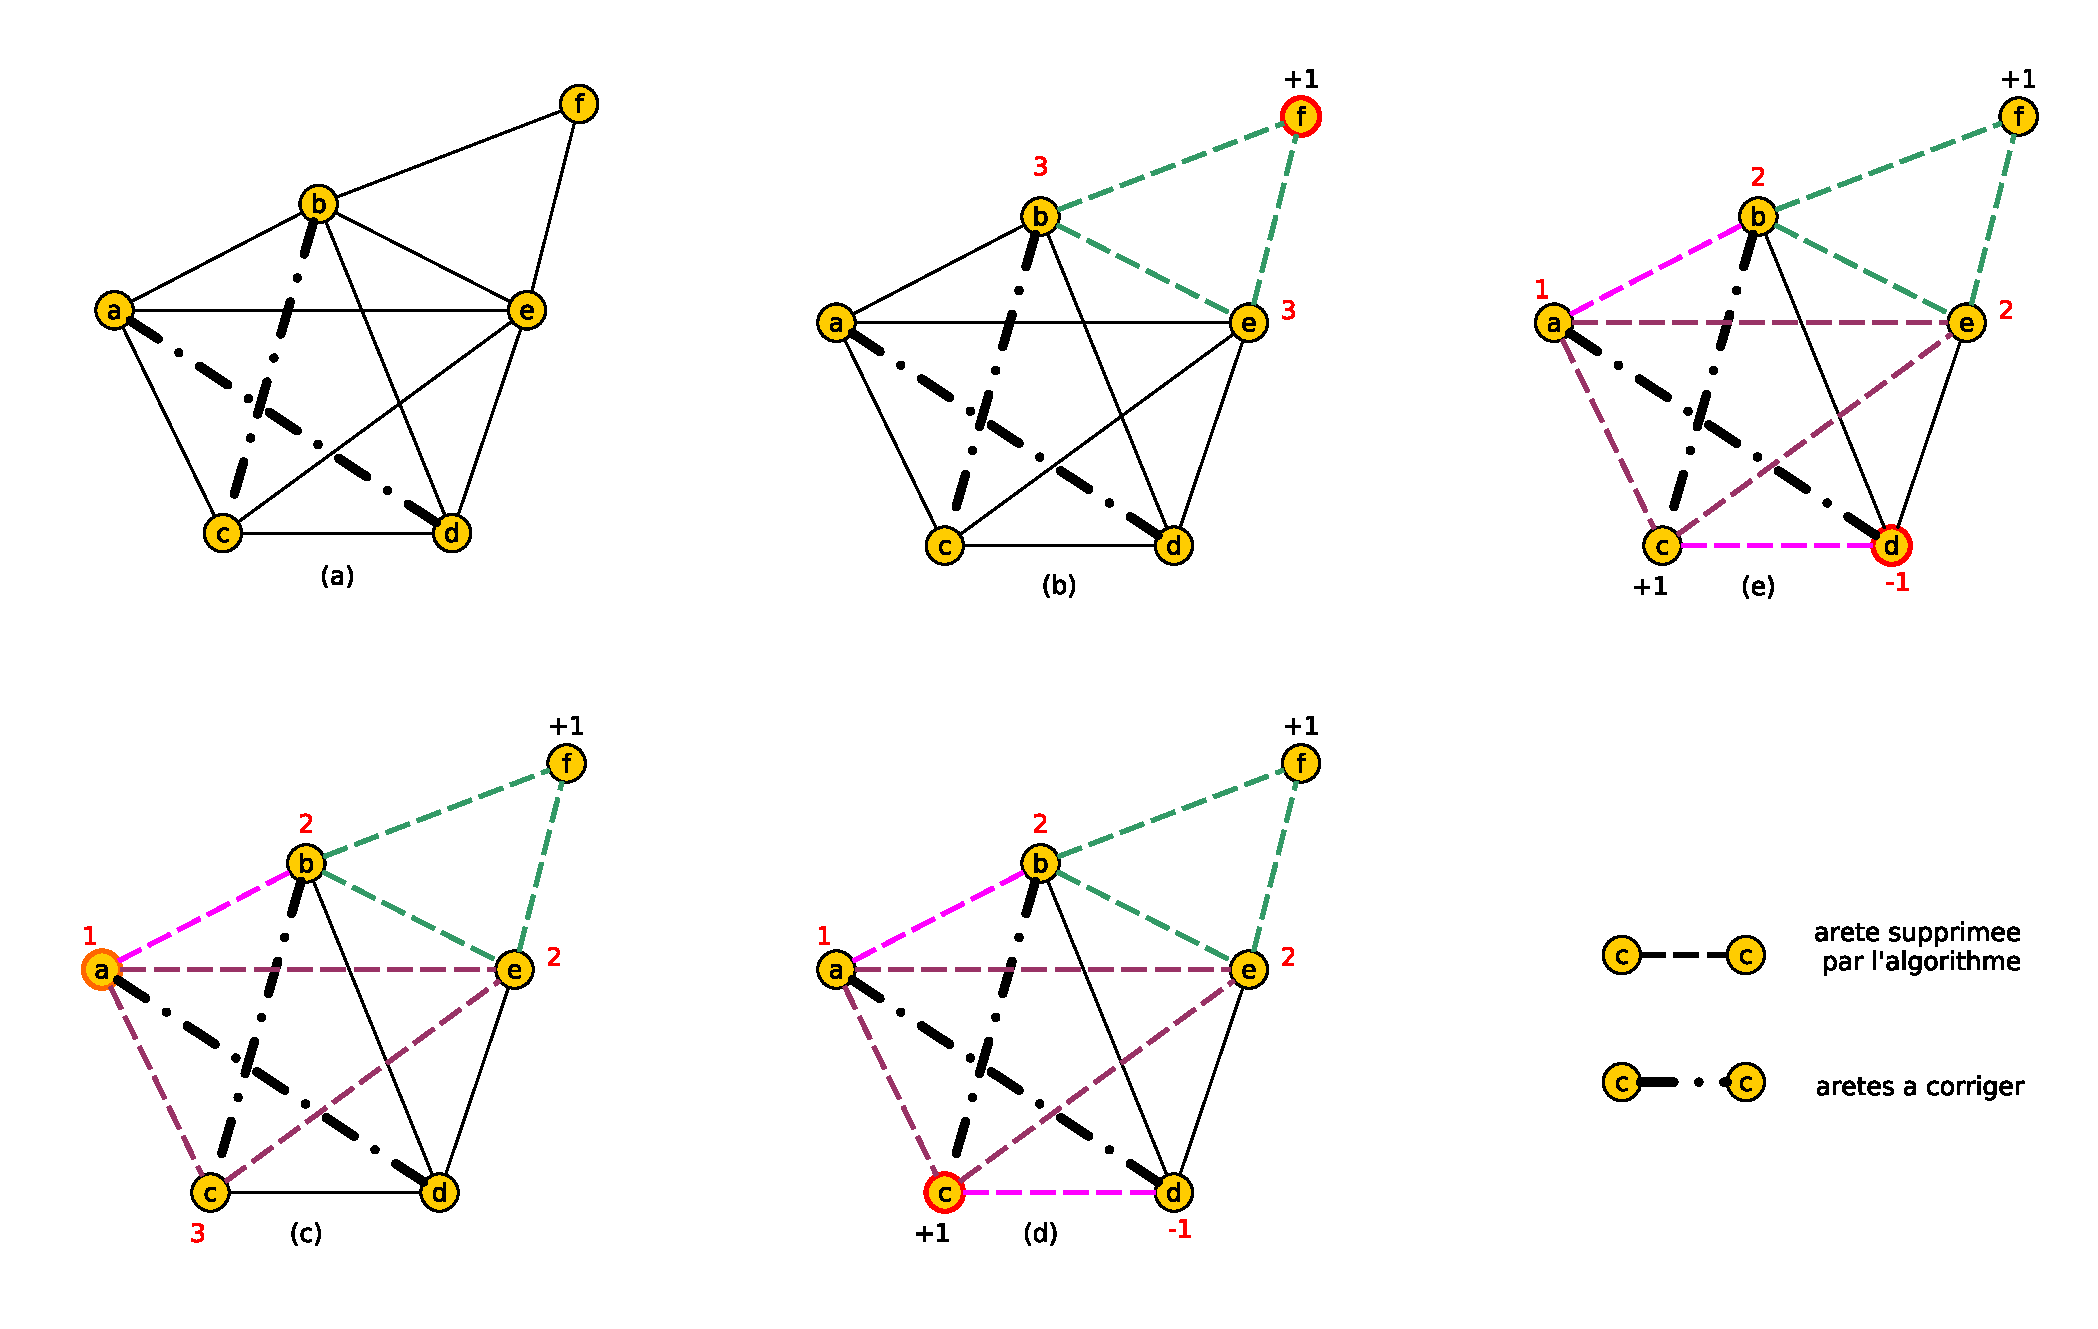
\includegraphics[width=500pt, height= 300pt]{exempleAlgorithmeCouverture.eps}\vspace{-0.5em}
	\caption{ Les diff\'erentes \'etapes de la couverture en cliques du graphe $G$. Les ar\^etes de m\^eme couleur appartiennent \`a la m\^eme clique.  Les ar\^etes $(b,c)$ et $(a,d)$ sont supprim\'ees du graphe avant l'ex\'ecution de l'algorithme de {\em couverture}.  }\vspace{-0.5em}
	\label{exempleAlgorithmeCouverture}
\end{figure}
%% ---- figure etapes de decouverte de l'algo de lehot
\FloatBarrier
%% description de l'algo
L'algorithme de recherche de couverture de corr\'elation ${\cal CC}(G_c)$ (voir algorithme \ref{algo:couverture})  consid\`ere, tant qu'il en existe, un sommet $v$ dont les ar\^etes incidentes sont couvertes par une seule clique. 
Il affecte \`a ce sommet l'\'etat $Cliq(v) = 1$, sauvegarde cette clique dans ${\cal CC}(G_c)$ puis supprime ces ar\^etes incidentes dans le graphe $G_c$. Les voisins de ce sommet passent \`a l'\'etat $2$.
\newline
Si au cours de l'ex\'ecution un tel sommet $v$ n'existe pas alors l'algorithme de {\em couverture} consid\`ere un sommet $u$ dont son voisinage peut \^etre couvert par deux cliques et qui n'a pas \'et\'e pr\'ec\'edemment couvert par une clique de ${\cal CC}(G_c)$. 
Si cette partition en deux cliques est unique, l'algorithme affecte $Cliq(u) = 1$ \`a ce sommet et supprime les ar\^etes. 
Dans le cas o\`u ce sommet appartient \`a un des cas de la figure \ref{configurationAmbiguite} (cas d'un sommet encadr\'e), nous avons montr\'e que ces graphes sont les seuls line-graphes pour lesquels deux partitions possibles existent. 
Nous utilisons la fonction de d\'ecision  $Verif-correl$  (section \ref{VerifCorrel}) pour lever l'ambigu\"{i}t\'e.
\newline
Un \'etat est affect\'e aux autres sommets $v$ de la clique couvrant $v$ selon l'un des trois cas. 
Dans le premier cas, l'\'etat actuel appartient \`a $Cliq(v) \in \{2,3\}$ si les sommets $v$ ont des ar\^etes incidentes non encore couvertes par une clique et l'\'etat pr\'ec\'edent est $Cliq(v) \in \{ 3,0\}$. 
Dans le second cas, $Cliq(v) = 1$ est attribu\'e aux sommets $v$ si l'ensemble des ar\^etes incidentes est vide. 
Enfin, dans le dernier cas, l'algorithme  affecte $Cliq(v) = -1$ \`a ces sommets si leur \'etat pr\'ec\'edent est  $Cliq(v) \in \{2,3\}$ et leurs ar\^etes incidentes ne forment pas une clique.
\newline
\`A la fin  de l'ex\'ecution de cet algorithme, tous les sommets $v$ dont l'\'etat courant est $Cliq(v) = -1$  n'ont pas \'et\'e couverts. 
Ces sommets appartiennent \`a l'ensemble $\cal C$ des sommets \`a corriger par l'algorithme de correction.
\newline

 La figure \ref{exempleAlgorithmeCouverture} d\'etaille l'algorithme de {\em couverture} (algorithme \ref{algo:couverture})  sur un graphe $G=(V,E)$  dans lequel nous avons supprim\'e deux ar\^etes. L'objectif de la suppression d'ar\^etes dans la figure \ref{exempleAlgorithmeCouverture}(a) est d'obtenir des sommets \`a corriger \`a la fin de la couverture.
 Nous s\'electionnons le sommet $f$ car il est de degr\'e minimum. 
 Il forme une clique avec son voisinage alors la clique $\{f,b,e\}$ est ajout\'ee \`a l'ensemble  ${\cal CC}(G)$ puis les ar\^etes $(f,b), (b,e), (f,e)$ sont supprim\'ees de $E$. 
 L'\'etat de $f$ est $Cliq(f) = 1$ et les sommets $b$ et $e$ ont $Cliq(b) = Cliq(e) = 3$ (voir figure \ref{exempleAlgorithmeCouverture}(c)). 
 \newline
 Le second sommet trait\'e est $a$ car son \'etat est $Cliq(a) = 0$. Il existe deux partitions coh\'erentes $\{a,b\}$ et $\{a,e,c\}$ au voisinage de $a$. Ces deux partitions sont ajout\'ees \`a    ${\cal CC}(G)$ et les ar\^etes de ces cliques sont supprim\'ees de $E$. L'algorithme attribue 
 \begin{itemize}
\item  Au sommet $a$, l'\'etat $Cliq(a) = 1$,
\item Aux sommets $b$ et $e$, les \'etats $Cliq(b) = Cliq(e) = 2$ car leur \'etat pr\'ed\'ecent \'etait $Cliq(b) = Cliq(e) = 3$ et ces sommets ont encore un voisin,
\item Au sommet $c$, l'\'etat $Cliq(b) = 3$.
 \end{itemize}
 On traite les autres sommets ($c$) de la m\^eme mani\`ere jusqu'\`a ce qu'on s\'electionne le sommet $d$.
 Ce sommet a deux partitions $\{d,b\}$ et $\{d,e\}$ non coh\'erentes (voir d\'efinition \ref{cliquesCoherentes}) parce que la fonction $Verif-correl$ (section \ref{VerifCorrel}) appliqu\'ee \`a ces partitions retourne 0. 
 Ce sommet est donc \`a corriger ${\cal C} = \{d\}$ (voir figure \ref{exempleAlgorithmeCouverture}(e)).
\newline

Si le graphe $G_c=(V_c, E_c)$ est un graphe de corr\'elation alors l'algorithme de couverture en d\'etermine la couverture de corr\'elation ${\cal CC}(G_c)$.
En effet, si $G_c$ est un line-graphe, par r\'ecurrence sur l'ensemble des sommets et \`a chaque \'etape, il existe un sommet non encore couvert qui :
\begin{itemize}
\item Soit est couvert par une clique appartenant \`a ${\cal CC}(G_c)$ et son voisinage restant peut \^etre convert par une nouvelle clique.
\item Soit n'est couvert par aucune clique de  ${\cal CC}(G_c)$ et son voisinage restant peut \^etre couvert par une ou deux nouvelles cliques.
\item Soit est dans une ambigu\"{i}t\'e alors on a recours \`a la fonction $Verif-correl$ (section \ref{VerifCorrel}) pour d\'eterminer les bonnes partitions de ce sommet.
\end{itemize}

\subsubsection{Complexit\'e de l'algorithme de couverture}

Si $G_c$ est un line-graphe, le sommet choisi $u$ (s'il existe) \`a la ligne $4$ de l'algorithme \ref{algo:couverture}  est \`a l'\'etat $Cliq(u) = 0$ et le sommet $u$ n'est pas un sommet ambigu. Dans le cas contraire, il est \`a l'\'etat $Cliq(u) = 3$.
Chaque s\'election de sommets conduit \`a  une unique et correcte partition et aussi \`a une seule couverture de corr\'elation. 
Nous montrons par induction sur l'ensemble des sommets qu'\`a chaque \'etape de l'algorithme \ref{algo:couverture}, il y a un sommet :
\begin{itemize}
	\item Non couvert par aucune clique et certains de ses voisins peuvent \^etre couverts par $1$ ou $2$ nouvelles cliques ($Cliq(u) = 0$, voir graphe $(b)$ de la figure \ref{exempleAlgorithmeCouverture}).
	\item Couvert par une clique d\'ej\`a dans la couverture de corr\'elation ${\cal CC}$ et ses voisins non couverts peuvent \^etre couverts par une nouvelle clique  ($Cliq(u) = 3$, voir graphe $(c)$ de la figure \ref{exempleAlgorithmeCouverture}).
\end{itemize} 
L'algorithme de couverture d\'etermine la couverture de corr\'elation si $G_c$ est v\'eritablement un line-graphe.

En revanche, si le graphe $G_c$ n'est pas un line-graphe alors, \`a certaines \'etapes, deux diff\'erents m\'ethodes de couvrir le sommet choisi par des cliques peuvent se pr\'esenter. Dans certains cas, nous choisissons al\'eatoirement  une des m\'ethodes (cela peut avoir un impact sur l'algorithme de correction). 
Notons que nous r\'ealisons les m\^emes op\'erations si le graphe $G_c$ est non connexe, m\^eme si des composantes connexes sont isomorphes aux graphes de la figure  \ref{neufSousGraphesInterditDesLineGraphes}. 
Le line-graphe obtenu est toujours un graphe connexe.
\newline

Concernant la complexit\'e, d\'eterminer si un sommet $u$ de $G_c$ est couvert par $1$ ou $2$ cliques a une complexit\'e de $O(\Delta(G_c)^2)$ (en d\'eterminant si le nombre chromatique du graphe compl\'ementaire est $1$ ou $2$). 
Alors la complexit\'e de l'algorithme de couverture est dans le pire des cas $O(n \times \Delta(G_c)^2)$ avec $n$ le nombre de sommets.  
Rappelons que l'algorithme de Lehot \cite{decompositionEnCliquesParArcs} a une complexit\'e de $O(n \times \Delta(G_c))$. Cependant, il ne fournit pas de couverture de corr\'elation partielle lorsque  $G_c$ n'est pas un line-graphe.
\newline

{\bf Conclusion} : si le graphe $G_c$ est un line-graphe, tous ses sommets $v$ sont labellis\'es \`a $Cliq(v) = 1$ et l'algorithme  de {\em couverture} trouve une partition du voisinage d'un sommet en une ou deux cliques de fa\c con unique (voir les lemmes pr\'ec\'edents). 
Une fois ce sommet et ses ar\^etes incidentes supprim\'ees, le graphe restant est toujours un line-graphe, et la propri\'et\'e se propage.
%Donc, si $G_c$ est un line-graphe, cet algorithme en trouvera toujours la couverture de corr\'elation unique.
Ainsi $G_c$ qui poss\`ede des sommets $v$ aux \'etats $Cliq(v) = -1$ n'est pas un line-graphe. Nous proposons l'algorithme de correction qui retourne le line-graphe le plus proche de $G_c$.


%---------------------------- algorithme de couverture ---------------------------------------------------------------------
\begin{algorithm}
\algsetup{indent=2em}
\caption{Couverture}
\label{algo:couverture}
\begin{algorithmic}[1]
\IF{$G_c$ est isomorphe \`a un graphe double (voir figure \ref{graphe2Couverture})}
	\STATE{le traiter avec $Verif-correl$ $(^1)$}
\ELSE
	\WHILE {il existe un sommet $u$ t.q $Cliq(u) \in \{0,3\}$}
		\STATE{ choisir un sommet $u$ de degr\'e minimum}
		\IF{ $\{u\} \cup \Gamma_{G_c}(u)$ peut \^etre couvert par deux cliques $C_1$ et $C_2$ coh\'erentes, \\ ~~~~~~$C_1$ maximale et $C_2 = \emptyset$ si $Cliq(u)=3$ $(^2)$ }
			\IF{$Cliq(u) = 0$ et $C_2 \neq \emptyset$}
				\STATE{ $Cliq(u)= 3$ }
			\ELSE
				\IF{$Cliq(u) = 0$ et $C_2 =  \emptyset$}
					\STATE{$Cliq(u) = 1$}
				\ELSE
					\STATE{$Cliq(u) = 2$}
				\ENDIF
			\ENDIF
			\STATE{ $\epsilon_u = E(G_c[C_1]) \cup E(G_c[C_2])$ }
			\FOR{$w \in \Gamma_{G_c}(u)$}
				\STATE{ $\alpha(w) = card\{[w,x] \in E - \epsilon_u\}$}
				\IF{$\alpha_w > 0$}
					\IF{ $Cliq(w) = 0$ }
						\STATE{$Cliq(w) = 3$}
					\ELSE
						\IF{$Cliq(w) = 3$}
							\STATE{$Cliq(w) = -1$}
						\ENDIF	
					\ENDIF
				\ELSE
					\IF{$Cliq(w) = 0$}
						\STATE{$Cliq(w) = 1$}
					\ELSE
						\IF{$Cliq(w) = 3$}
							\STATE{$Cliq(w) = 2$}
						\ENDIF
					\ENDIF
				\ENDIF
			\ENDFOR
			\STATE{$E = E - \epsilon_{u}$}
		\ELSE
			\STATE{$Cliq(u) = -1$}
		\ENDIF
	\ENDWHILE
\ENDIF
\end{algorithmic}
\end{algorithm}
%
%\begin{algorithm}[!ht]
%\label{algo:couverture}
%\caption{couverture}
%%\begin{algorithmic}[1]
%\noindent DEBUT\\
%\noindent 1. {\bf Si} $G_c$ est isomorphe \`a un graphe double (voir figure \ref{graphe2Couverture} ), {\bf alors} le traiter avec Verif-correl$(^1)$ \\
%~~\indent {\bf Sinon} \\
%~2. \indent {\bf Tant que} il existe un sommet $u$ t.q $Cliq(u) \in \{0,3\}$\\ 
%       	\indent~~~~~~{\bf Faire}\\
%~3.	       	\indent~~~~~~~~choisir $u$ de degr\'e minimum\\
%~4.       	\indent~~~~~~~~{\bf Si} $\{u\} \cup \Gamma_{G_c}(u)$ peut \^etre couvert par deux cliques $C_1$ et $C_2$ coh\'erentes,\\
%		\indent~~~~~~~~~~~~~~$C_1$ maximale et $C_2 = \emptyset$ si $Cliq(u)=3$ $(^2)$\\
%	       	\indent~~~~~~~~~~~~{\bf alors}\\
%~5.	       	\indent~~~~~~~~~~~~~~{\bf Si } $Cliq(u) = 0$ et $C_2\neq \emptyset$ {\bf Alors} $Cliq = 3$ \\
%~6.		\indent~~~~~~~~~~~~~~{\bf Sinon Si} $Cliq = 0$ et $C_2 =  \emptyset$ {\bf Alors} $Cliq(u) = 1$\\
%~7.		\indent~~~~~~~~~~~~~~~~~~~~~~~{\bf Sinon} $Cliq(u) = 2$ 	\\
%~8.		\indent~~~~~~~~~~~~~~~~~~~~~~~{\bf FinSi}\\      	
%~9.		\indent~~~~~~~~~~~~~~{\bf FinSi}\\
%~10.		\indent ~~~~~~~~~~~~~$\epsilon_u = E(G_c[C_1]) \cup E(G_c[C_2])$\\
%~11.		\indent ~~~~~~~~~~~~~{\bf Pour tout} $w \in \Gamma_{G_c}(u)$ {\bf Faire} \\
%~12.		\indent~~~~~~~~~~~~~~~~$\alpha(w) = card\{[w,x] \in E - \epsilon_u\}$\\
%~13.		\indent~~~~~~~~~~~~~~~~{\bf Si} $\alpha_w > 0$ {\bf Alors}\\
%~14.		\indent~~~~~~~~~~~~~~~~~~{\bf Si} $Cliq(w) = 0$ {\bf Alors} $Cliq(w) =3$\\
%~15.		\indent~~~~~~~~~~~~~~~~~~{\bf Sinon Si} $Cliq(w) = 3$ {\bf Alors} $Cliq(w) =-1$\\
%~16.		\indent~~~~~~~~~~~~~~~~~~{\bf FinSi} \\
%~17.		\indent~~~~~~~~~~~~~~~~{\bf Sinon Si} $Cliq(w) = 0$ {\bf Alors} $Cliq(w) =1$\\
%~18. 	\indent~~~~~~~~~~~~~~~~~~~~~~~~~{\bf Sinon Si} $Cliq(w) = 3$ {\bf Alors} $Cliq(w) = 2$ \\
%~19. 	\indent~~~~~~~~~~~~~~~~~~~~~~~~~{\bf FinSi} \\
%~20.		\indent ~~~~~~~~~~~~~{\bf FinPourTout}\\
%~21.		\indent ~~~~~~~~~~~~~$E = E - \epsilon_u$\\
%~22.		\indent            ~~~~~~~{\bf Sinon} $Cliq(u) = -1$\\
%	       	\indent~~~~~~~~~~~~{\bf FinSi}\\
%%       	\indent~~~~~~
%~23. \indent {\bf FinTant que}\\
%~24. \noindent {\bf Fin Si}\\
%\noindent FIN\\
%%\end{algorithmic}
%\end{algorithm}
%---------------------------- algorithme de couverture ---------------------------------------------------------------------

\FloatBarrier
$^1$ : chaque graphe de la figure \ref{graphe2Couverture} admet deux couvertures de corr\'elation, souvent isomorphes, mais une seule de ces couvertures de corr\'elation peut correspondre au DAG du r\'eseau \'electrique sous-jacent. Dans ce cas, on utilise la fonction $Verif-correl$ afin de d\'eterminer la couverture de corr\'elation la plus probable.
\newline

 $^2$ :  le sommet $u$ choisi (s'il existe) ne sera pas prioritairement un sommet tel que $Cliq(u) = 0$ et $u$ est un point d'ambigu\"{i}t\'e. Si lors d'une \'etape, seul un tel choix est possible et qu'il n'y a aucun sommet $u$ tel que $Cliq(u) = -1$, c'est que chaque sommet du graphe initial $G_c$ est un point d'ambigu\"{i}t\'e.
 Dans ce cas, $G_c$ est une union de composantes connexes isomorphes \`a un des graphes de la figure  \ref{graphe2Couverture}.
Dans ce cas, n'importe quel choix conduit \`a une couverture de corr\'elation correcte.

		
	%------- algo correction -----------------------------------------------
	\subsection{Algorithme de correction}
		%Si le graphe $G_c=(V_c, E_c)$ est un graphe de corr\'elation alors l'algorithme de couverture en d\'etermine une couverture de corr\'elation $\cal H$.
%En effet, si $G_c$ est un line-graphe, on montre, par r\'ecurrence sur l'ensemble des sommets et \`a chaque \'etape, qu'il existe un sommet non encore couvert qui :
%\begin{itemize}
%\item soit est couvert par une clique appartenant \`a $\cal H$ et son voisinage restant peut \^etre convert par une nouvelle clique.
%\item soit n'est couvert par aucune clique de  $\cal H$ et son voisinage restant peut \^etre couvert par une ou deux nouvelles cliques.
%\end{itemize}
%Dans le cas o\`u la couverture de corr\'elation de $G_c$ ne peut \^etre fournie \`a cause des cases erronn\'ees de la matrice d'adjacence de $G_c$, nous avons des sommets couverts par soit aucune clique ou soit par plus de deux cliques. Ces sommets, labellis\'es \`a $-1$, forment l'ensemble 
%$sommets\_1 = \{\exists z \in V, Cliq(z) = -1 \}$ 
%et sont appel\'es {\em sommets \`a corriger}.
%Dans le cas o\`u $G_c$ contient des cases erronn\'ees dans sa matrice d'adjacence, la couverture de corr\'elation ne peut \^etre propos\'ee. N\'eanmoins, $\cal H$ contient seulement les cliques qui couvrent les sommets labellis\'es \`a $Cliq = 1$. Les sommets \`a   $Cliq = -1$  forment l'ensemble $\cal C$ des sommets \`a corriger et ce sont ces sommets qui sont trait\'es par l'algorithme suivant.
\label{algorithmeCorrection}
Nous l'avons vu, si $G_c=(V_c, E_c)$ n'est pas un line-graphe, certains sommets ne peuvent pas \^etre converts par $1$ ou $2$ cliques. Dans l'algorithme de couverture, ces sommets $v$ sont labellis\'es par $Cliq(v) = -1$. 
L'ensemble des cliques ${\cal CC}(G_c)$ ne contient alors que des cliques dans lesquelles les sommets $v$ labellis\'ees \`a $Cliq(v)=1$ sont couverts par $1$ ou $2$ cliques. 
Les sommets $v$ dont l'\'etat $Cliq(v) = -1$ appartiennent \`a l'ensemble $\cal C$ des sommets \`a corriger et ce sont ces sommets qui sont trait\'es par l'algorithme suivant.
\newline

Nous proposons l'{\em algorithme de correction} qui va modifier l'ensemble initial $E_c$ par l'ajout et la suppression d'ar\^etes dans le but d'obtenir un {\em line-graphe}.
Dans cet algorithme, nous traitons un sommet de $\cal C$ apr\`es l'autre sachant que chaque sommet peut modifier $\cal C$.
Soit $z_i$ le $i^{ieme}$ sommet trait\'e dans ${\cal C}$.
Certaines exp\'eriences r\'ealis\'ees dans le chapitre \ref{chapitreEvaluation} montrent que 
 le choix des sommets \`a traiter, \`a chaque \'etape de correction, peut avoir une influence sur le line-graphe fourni parce que la correction modifie le voisinage des sommets.
 Nous notons alors 
 $E_c^i$ l'ensemble des ar\^etes de $G_c$ apr\`es le traitement du $(i-1)^{ieme}$ sommet de ${\cal C}$ et 
 ${\cal CC}^{i}(G_c)$ l'ensemble des cliques de $G_c$ \`a l'\'etape $i$. 
 Ainsi $E_c^1 = E_c$ et ${\cal CC} = {\cal CC}(G_c) = {\cal CC}^{1}(G_c)$. 
 Nous notons ${\cal CC}$ pour d\'esigner ${\cal CC}(G_c)$ dans la suite de cette section.
 \newline


Soient $z_i$ le $i^{ieme}$ sommet et ${\cal CC}(z_i) = \{C_1, \cdots, C_k\}$ l'ensemble des cliques maximales de ${\cal CC}^i$ de taille sup\'erieure ou \'egale \`a $3$ auxquelles le sommet $z_i$ appartient.
Notons que, par d\'efinition et par construction, chaque paire de cliques dans ${\cal CC}(z_i)$ n'a que $z_i$ comme sommet commun et que $S(z_i)$ est l'union des voisins $v$ de $z_i$ dans des cliques $\{v,z_i\} \in {\cal CC}^i$ de taille $2$ et des voisins $v$ de $z_i$ tels que l'ar\^ete $[z_i,v]$ n'est couverte par aucune clique de ${\cal CC}^i$.
\begin{equation}
C(z_i) = \{C_i, i \in [1,k] \mid  |C_i| \ge 3 \mbox{ } \&  \mbox{ } C_i \in {\cal CC}^i \} 
\end{equation}
\begin{equation}
S(z_i) = \{v \in \Gamma_{G_c}(z_i) \mid \{v,z_i\} \in {\cal CC}^i\} \cup  \{ v \in \Gamma_{G_c}(z_i) \mid \nexists C \in {\cal CC}^{i} , [z_i,v] \in E_c(C) \}
\end{equation}

\begin{definition}
Soient 
${\cal CC}^{i}$ la couverture de corr\'elation apr\`es le traitement des $(i-1)^{ieme}$ sommets de ${\cal C}$ et
${\cal CC}^{i}(z_i)$ l'ensemble des cliques contenant le $i^{ieme}$  sommet $z_i$.
\newline
Deux cliques $C$ et $C'$ de ${\cal CC}^{i}(z_i)$ sont {\bf contractables} si aucune ar\^ete $[u,v]$ de $E_c^i$ telle que $u \in C$ et $v \in C'$ n'est couverte par une clique (autre que ${u,v}$) dans ${\cal CC}^{i}$.
Un ensemble de cliques de ${\cal CC}^{i}$ est contractable si tous les cliques sont deux \`a deux contractables.
\end{definition}
% mettre un exemple de cliques contractables et aussi ce cas C et $emptyset$ sont contractables
Dans la figure \ref{exempleAlgoCorrectionGraphe}(a), les paires de cliques $(C3, C4)$, $(C2, C3)$ sont contractables car il n'y a aucune ar\^ete entre les sommets $5$ et $6$ dans la premi\`ere paire et dans la seconde paire, les sommets $3$ et $4$ n'ont aucune ar\^ete entre eux. 
Cependant, la paire $(C4, C6)$ n'est pas contractable car l'ar\^ete $[z_i,10]$ est couverte par la clique $C5$. De m\^eme, la clique $C1$ n'appartenant pas \`a ${\cal CC}^{i}(z_i)$ entraine que les cliques $C1$ et $C2$ ne sont pas contractables.

\begin{definition}
Soient 
${\cal CC}^{i}$ la couverture de corr\'elation apr\`es le traitement des $(i-1)^{ieme}$ sommets de ${\cal C}$ et
${\cal CC}^{i}(z_i)$ l'ensemble des cliques contenant le $i^{ieme}$ sommet $z_i$.
\newline
Une clique $C \in {\cal CC}^{i}$ est {\bf voisine} de $z_i$ si $C \notin {\cal CC}^{i}(z_i)$ et $card(C \cap S(z_i)) \ge 1$.
La d\'ependance d'une clique $C$ voisine de $z_i$ est l'ensemble $D_{z_i}(C) \subset {\cal CC}^{i}(z_i)$ tel que $C' \in D_{z_i}(C)$ si et seulement si  $C' \cap C \cap \Gamma_{G_c}(z_i) \ne \emptyset$.
\newline
Une clique $C$ est {\bf augmentante} pour le sommet $z_i$ si et seulement si elle est voisine de $z_i$ et  $D_{z_i}(C)$ est vide  ou $D_{z_i}(C) \cup \{C\}$ est contractable.
\begin{equation}
voisine(z_i) = \{C \in {\cal CC}^{i} \mbox{ } \mid \mbox{ } C \notin C(z_i) \mbox{ } \& \mbox{ } card(C \cap S(z_i)) \ge 1 \} \newline
\end{equation}
\begin{equation}
D_{z_i}(C) = \{ C' \in C(z_i) \mbox{ } \mid  \mbox{ } C' \cap C \cap \Gamma_{G_c}(z_i) \ne \emptyset \}
\end{equation}
\end{definition}
% mettre un exemple de cliques voisine et dependantes.

On appelle {\bf  augmentation} du sommet $z_i$ l'union d'une clique augmentante  $C$ pour $z_i$ et d'une contraction de cliques de $D_{z_i}(C)$.
\newline

Dans notre exemple, consid\'erons  $\overbar{C}(z_i) = \{C1, C6\}$  les cliques n'appartenant pas \`a ${\cal CC}^{i}(z_i)$ et $S(z_i) = \{10,1\}$.
L'ensemble des cliques voisines \`a $z_i$ est $voisine(z_i) = \{C1, C6\}$ parce que l'intersection de $C1$ et $S(z_i)$ donne un sommet $\{1\}$ et celle de $C6$ et $S(z_i)$ donne un sommet $\{10\}$
($C1 \cap S(z_i) = \{1,2,11\} \cap \{10,1\} = \{1\}$,
$C6 \cap S(z_i) = \{8,9,10\} \cap \{10,1\} = \{10\}$
).
Par ailleurs, la d\'ependance de la clique $C1$ est $D_{z_i}(C1) = C2$ ($C1 \cap C2 \cap \Gamma_{G_c}(z_i) = \{2\}$) et celle de $C6$ est $D_{z_i}(C6) = C4$ ($C6 \cap C4 \cap \Gamma_{G_c}(z_i) = \{8\}$). 
Nous en d\'eduisons que la clique $C1$ est {\em augmentante} car  $C1$ est contractable avec $C2$ et est voisine de $z_i$. De m\^eme, la clique $C6$ est {\em augmentante} car $C6$ est voisine de $z_i$ et puisque l'ar\^ete $[z_i,10]$ forme la clique $C5$, la paire $(C6,C4)$ est contractable.
Une {\em augmentation} de $z_i$ est soit $\{z_i\} \cup C1 \cup C2$ ou soit $\{z_i\} \cup C4 \cup C6$.
%Un exemple de clique augmentante $C1$ pour le sommet $z_i$ est donn\'e dans la figure \ref{exempleAlgoCorrectionGraphe}, avec $D_{z_i}(C1) = \{C2\}$.
%Par contre, la clique C6 ne peut pas \^etre augmentante \`a cause de l'appartenance de l'ar\^ete $[u,v]$ \`a la clique $C7$ de $C^i$. Ce qui rend impossible toute contraction entre $C6$ et $C4$
%% ------ figure correctionGraph
\begin{figure}[htb!]
\centering
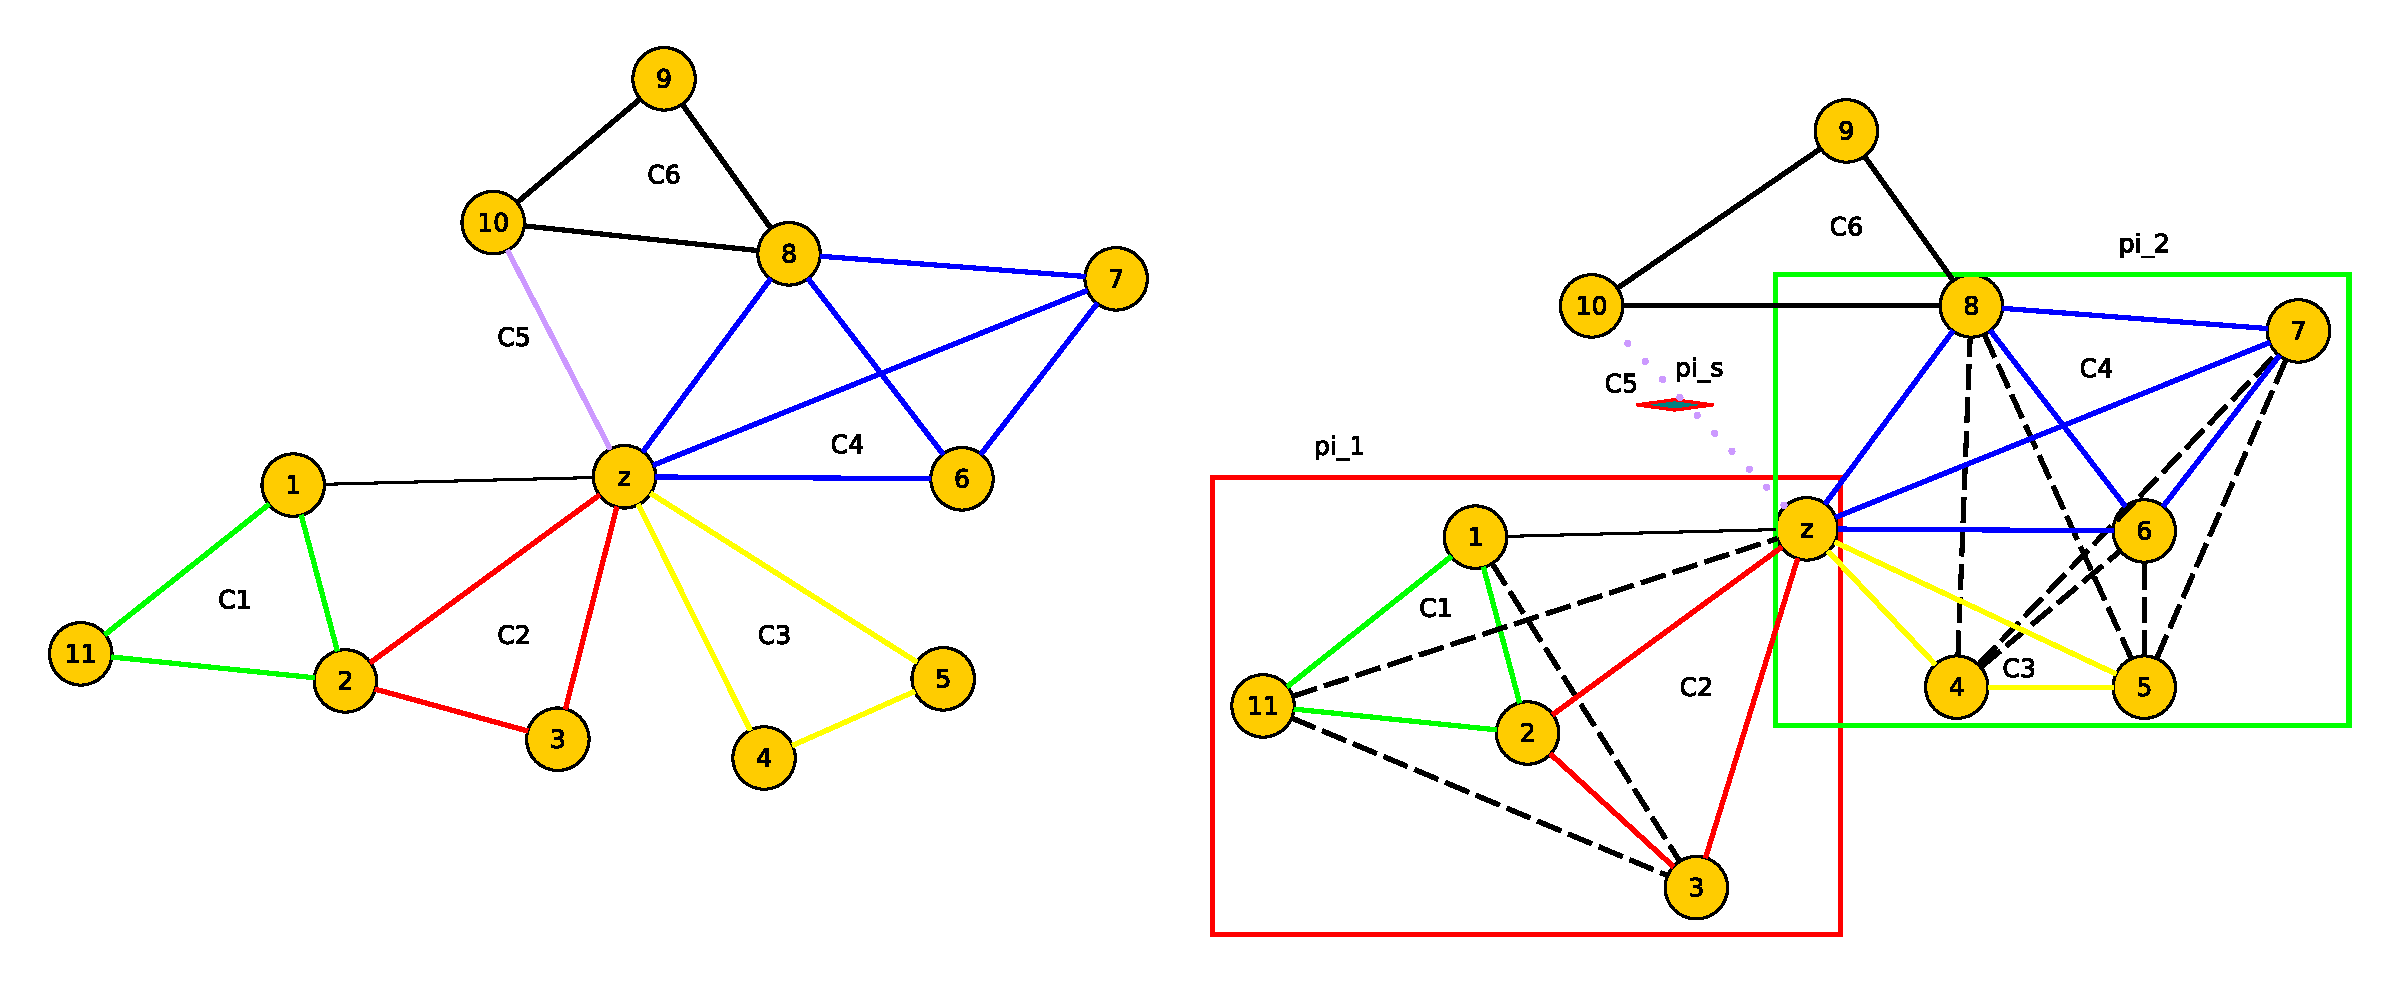
\includegraphics[scale=0.450]{./correctionGraph.eps} \vspace{-0.5em}
\caption{(a) Le sommet $z$ et son voisinage avec les cliques qui le couvrent , (b) un exemple de compression de cliques :  les sommets \`a l'int\'erieur des rectangles rouges et verts forment les nouvelles cliques couvrant $z$.
		$\pi_1 = \{1,2,3,z,11\}$, $\pi_2 = \{z,4,5,6,7,8\}$, $\pi_s = \{10\}$ 
		}
\label{exempleAlgoCorrectionGraphe}
\end{figure}
%% ------ figure correctionGraph
\FloatBarrier

Soient $\pi_1$, $\pi_2$ une bipartition du voisinage du sommet $z_i$  en cliques  et 
$\pi_s$ un ensemble  de sommets dont l'ar\^ete form\'ee par un de ces sommets et le sommet $z_i$ sont  \`a retirer du graphe $G_c$.  
\begin{definition}
Soient 
${\cal CC}^{i}$ la couverture de corr\'elation apr\`es le traitement des $(i-1)^{ieme}$ sommets de ${\cal C}$ et
${\cal CC}^{i}(z_i)$ l'ensemble des cliques contenant le $i^{ieme}$ sommet $z_i$.
\newline
On appelle {\bf compression} du sommet $z_i$ un triplet ($\pi_1$, $\pi_2$, $\pi_s$) d\'efini par : 
\begin{itemize}
	\item $\pi_1$ (resp. $\pi_2$) peut \^etre d'une des formes suivantes :
	\begin{enumerate}
		\item L'union de $z_i$, d'un sous-ensemble $C_1$ (resp. $C_2$) de cliques de ${\cal CC}^{i}(z_i)$ telle que toute paire $(C,C')$ de $C_1$ (resp. $C_2$) est contractable et d'un sous-ensemble $S_1$ (resp. $S_2$) de sommets $v \in S(z_i)$ n'appartenant \`a aucune clique de $C_1$ (resp. $C_2$) tel que
		$$ \forall v \in S_1,~\forall x \in C_1, \not\exists C' \in {\cal CC}^{i}~t.q.~card(C')>2~~et~~\{v,x\} \subset C'$$
		(ce qui fait que \{v,x\} peut \^etre une clique de ${\cal CC}^{i}$).
		\item Une augmentation du sommet $z_i$.
	\end{enumerate}
	\item L'intersection entre $\pi_1$ et $\pi_2$ est r\'eduite $\{z_i\}$ ($\pi_1 \cap \pi_2 = \{z_i\}$),
	\item $\pi_s=\Gamma_{G_c}(z_i)-~((\pi_1 \cap \Gamma_{G_c}(z_i) ) \cup(\pi_2 \cap \Gamma_{G_c}(z_i) ))$ tel que l'ensemble des ar\^etes  $\{[z_i,v]\in E_{c}^{i}:~v\in \pi_s\}$ n'est pas d\'econnectant.
	\item Le triplet $\pi_{1} \cap \Gamma_{G_c}(z_i)$, $\pi_{2} \cap \Gamma_{G_c}(z_i)$, $\pi_{s} \cap \Gamma_{G_c}(z_i)$  est une 3-partition de $\Gamma_{G_c}(z_i)$.
\end{itemize}
\end{definition}
Il existe toujours une telle compression, ne serait-ce que 
$\pi_1 = \{z_i\} \cup C_i \in C(z_i)$, 
$\pi_2 =  \emptyset$,
$\pi_s = \Gamma_{G_c}(z_i) -(\Gamma_{G_c}(z_i) \cup C_i) $  si ${\cal CC}^{i}(z_i)$ n'est pas vide.
Sinon, 
$\pi_1 = \{z_i\} \cup \{ v \in \Gamma_{G_c}(z_i)  \} $, 
$\pi_2 =  \emptyset$,
$\pi_s = \Gamma_{G_c}(z_i) - \{v\} $
est aussi une compression.
Un exemple de compression est aussi donn\'e dans la figure \ref{exempleAlgoCorrectionGraphe}.
Le co\^ut $c(T)$ d'une compression $\pi_{1},\pi_{2},\pi_{s}$ est d\'efini par : 
$$c(T) = | \{\{u,v\} \in \pi_{1}:~[u,v]\not\in E_{c}^{i}\}| + |\{\{u,v\} \in \pi_2:~[u,v]\not\in E_{c}^{i}\}| +~ |\pi_s| $$
%Dans l'exemple de la figure \ref{exempleAlgoCorrectionGraphe}(b), autour d'un sommet $z_i$, l'ensemble $C(z_i)$ contient les cliques $C2$, $C3$,$C4$ et $C5$.
%Les cliques $C5$ et $C4$ ne sont pas contractables, \`a cause de l'existence de $C6$ dans ${\cal C}_i$.
%La clique $C1$ est voisine de $z_i$ et $D_{z_i}(C1) = \{C2\}$.
L'exemple de la compression donn\'ee dans la figure \ref{exempleAlgoCorrectionGraphe}(b) est $\pi_1 = C1 \cup C2$ (une augmentation), $\pi_2 = C3 \cup C4$ (ces deux cliques \'etant contractables), et $\pi_s = \{10\}$.
Les cliques $C1$ et $C2$ sont compress\'ees en ajoutant les ar\^etes $[1,3]$ et $[z_i,11]$. De m\^eme, les cliques $C3$ et $C4$ sont compress\'ees en ajoutant les ar\^etes  $[4,8]$, $[5,8]$, $[7,4]$, $[7,5]$, $[6,4]$ et $[6,5]$. La clique $C5$ est supprim\'ee afin que $z_i$ ne soit pas couvert par trois cliques.
Le co\^ut  de cette compression est $10$, $10$ \'etant le nombre d'ar\^etes en pointill\'ees plus l'ar\^ete supprim\'ee $[10,z_i]$.
\newline

Soit  $c(T)$ le co\^ut minimum d'une compression $T$ de $z_i$.
Le but est de modifier $G_c$ afin que $z_i$ puisse \^etre couvert par une ou deux cliques issues de $\pi_1$ et $\pi_2$.
Pour cela, le co\^ut de cette modification $c(T)$ tient compte des ar\^etes \`a ajouter (li\'ees \`a $\pi_1$ et $\pi_2$) et \`a supprimer (li\'ees \`a $\pi_s$).
\begin{equation}
c(T) = \sum_{ \{u,v\} \subseteq \pi_1: [u,v] \notin E_c^i } \phi^{+}(u,v) + \sum_{ \{u,v\} \subseteq \pi_2: [u,v] \notin E_c^i } \phi^{-}(u,v) + \sum_{ v \in \pi_s } \phi^{-}(u,v)
\end{equation}
Avec $\phi^{+}$ le co\^ut de l'op\'eration {\em ajouter une ar\^ete} et  
$\phi^{-}$ le co\^ut de l'op\'eration {\em ajouter une ar\^ete}.
\newline
Nous \'evaluons les performances des diff\'erents couples de fonctions $\phi^{+}$ et $\phi^{-}$ dans le chapitre \ref{chapitreEvaluation}.
\newline

Ainsi, {\bf appliquer une compression} $T = \pi_1, \pi_2, \pi_s$ consiste \`a ajouter dans $E_c^i$ les ar\^etes d\'efinies par les ensembles de paires $\{\{u,v\} \in \pi_1:~[u,v]\not\in E_{c}^{i}\}$ (qui seront couvertes par la clique $\pi_1$) et $\{\{u,v\} \in \pi_2:~[u,v]\not\in  E_{c}^{i}\}$ (qui seront couvertes par la clique $\pi_2$) et \`a supprimer les ar\^etes $\{[z_i,v] \in  E_{c}^{i}:~v\in \pi_S\}$. 
\newline
D\`es lors, le sommet $z_i$ appartient aux deux cliques $\pi_1$ et $\pi_2$.
On proc\`ede alors aux mises \`a jour suivantes pour obtenir ${\cal CC}^{i+1}$ et $E_M^{i+1}$ :
\begin{itemize}
\item Supprimer toutes les cliques ${\cal CC}^{i}(z_i)$ couvertes par $\pi_1$ dans  ${\cal CC}^{i}$.
\item Supprimer toutes les cliques ${\cal CC}^{i}(z_i)$ couvertes par $\pi_2$ dans  ${\cal CC}^{i}$.
\item Supprimer toutes les cliques de cardinalit\'e $2$ couvertes par $\pi_1$ et $\pi_2$ dans  ${\cal CC}^{i}$.
\item Ajouter $\pi_1$ et $\pi_2$ dans ${\cal CC}^{i}$, supprimer de $E_c^{i+1}$ toutes les ar\^etes  $\{[z_i,v] \in E_c^{i}:~v\in \pi_s\}$.
\item Affecter $Cliq(z)$ \`a $1$ (si $\pi_1$  ou $\pi_2$ est vide) ou $2$ (sinon).
\end{itemize}
Cette proc\'edure a les propri\'et\'es suivantes :
\begin{property}
Consid\'erons l'application d'une compression.\newline
Soit ${\cal CC}^{i+1}$  l'ensemble obtenu \`a partir de ${\cal CC}^{i}$ apr\`es  la mise \`a jour selon cette application.
\begin{itemize}
	\item Tout sommet de $G_c$ couvert par une ou deux cliques dans ${\cal CC}^{i}$ le reste dans ${\cal CC}^{i+1}$.
	\item Toute ar\^ete couverte par une et une seule clique dans ${\cal CC}^{i}$ et qui n'est pas supprim\'ee le reste dans ${\cal CC}^{i+1}$.
	\item Le sommet $z_i$ est couvert par une ou deux cliques dans ${\cal CC}^{i+1}$ (le nombre de sommets ainsi couverts augmente de $1$ par rapport \`a celui dans ${\cal CC}^{i}$).
\end{itemize}
\end{property}

Ainsi, pour chaque sommet $z_i$, on consid\`ere une compression de co\^ut minimum $c_m^i$ et on l'applique.
La propri\'et\'e ci-dessus garantit qu'\`a la fin du processus, on obtient un graphe de corr\'elation $G_c^t = (V_c, E_c^t)$ dont l'ensemble ${\cal CC}^{i}$ modifi\'e est une couverture de corr\'elation.
Consid\'erons la distance de correction $DC(G_c^0, G_c^t ) = | (E_c^0 \cup E_c^t)  - (E_c^0 \cap E_c^t) |$ qui est le nombre de cases modifi\'ees dans la matrice d'adjacence du graphe $G_c$.
La distance-line v\'erifie  
$$DL( G_{c}^{0}, G_{c}^{t}) \le  DC(G_c^0, G_c^t ) $$
Notons que lors d'une \'etape $j > 1$, le sommet $z_j$ et son voisinage se retrouvent \^etre couvert par une ou deux cliques suite au traitement des $j-1$ sommets pr\'ec\'edents, aucune compression ne lui est appliqu\'ee (on consid\`ere la compression identit\'e) et donc 
$c_{m}^{j} = 0$.

	%------- Complexite algorithmes -----------------------------------------------
	\subsection{Complexit\'e des algorithmes}
		L'algorithme de correction traite au plus une fois chaque sommet du graphe.
La complexit\'e de traitement de chaque sommet est exponentielle en fonction du degr\'e de chaque sommet et des cliques auxquelles il appartient, la encore en fonction  de son degr\'e en taille et en nombre.
L'algorithme global (couverture et correction) est donc pseudo-polynomial en fonction du degr\'e du graphe.
\newline

Nous d\'eterminons une conjecture sur le comportement de l'algorithme.
\'Etant donn\'e un graphe de d\'epart, une ex\'ecution de l'algorithme est un ordre dans lequel seront trait\'es les sommets dans l'algorithme de couverture, puis
la s\'election des sommets $z_i$ \`a traiter dans  $\cal C$.
\newline
Consid\'erons un graphe de corr\'elation $G_c$ n'\'etant pas isomorphe \`a un graphe de la figure \ref{graphe2Couverture}. On dira que $G_c$ est non-ambigu.

Deux ar\^etes $[u,v]$ et $[u',v']$ de $G_c$ seront dit {\bf clique-independantes} si et seulement si il n'existe pas de cliques $C$ dans la couverture de corr\'elation  de $G_c$ telle que 
$C \cap \{u,v\} \cap \{u',v'\} \ne \emptyset$

\begin{conjecture}
Si $G'=(V, E')$ est un graphe obtenu en supprimant un ensemble d'ar\^etes deux \`a deux clique-independantes d'un graphe de corr\'elation non-ambigu $G_c = (V,E_c)$, alors il existe une ex\'ecution de l'algorithme qui transforme $G'$ en $G_c$.
\end{conjecture}


	%------- Conclusion description algorithmes -----------------------------------------------
	\subsection{Conclusion de la description des algorithmes}
		% --- a supprimer ce commenntaire cest une redite de l'algorithme de couverture
%Dans cette section, nous d\'ecrivons deux algorithmes. 
%Le premier algorithme est {\em l'algorithme de couverture} et il est bas\'e sur l'algorithme de Lehot \cite{decompositionEnCliques}. L'algorithme consid\`ere que chaque sommet peut avoir $4$ \'etats. Le premier \'etat $Cliq = 1$ est attribu\'e \`a des sommets couverts par une clique ou deux cliques et qui n'a aucune ar\^ete incidente. Le second \'etat $Cliq = 2$ est attribu\'e \`a des sommets couverts par une clique et qui poss\`ede des ar\^etes incidentes. Le troisi\`eme \'etat $Cliq = 3$ est attribu\'e \`a des sommets initialement n'ayant aucun \`etat ($Cliq=0$) et couvert par une clique. Et  le dernier \'etat $Cliq = -1$  est attribu\'e \`a des sommets couverts par deux cliques ayant des ar\^etes incidentes ou un sommet ayant des ar\^etes incidentes qui ne forme pas une clique. 
%\`A la fin de l'algorithme, les cliques d\'ecouvertes sont stock\'ees dans la line-couverture $\cal H$ et les sommets dont l'\'etat est $Cliq = -1$ sont contenus dans l'ensemble $\cal C$ des sommets \`a corriger.


Dans cette section, nous d\'ecrivons deux algorithmes. 
Le premier algorithme est {\em l'algorithme de couverture} qui attribue un \'etat \`a un sommet du graphe de corr\'elation en fonction des cliques qui le couvrent. L'ensemble de cliques est la couverture de corr\'elation ${\cal CC}$. La particularit\'e de la couverture de corr\'elation est que chaque sommet appartient \`a $1$ ou $2$ cliques. Lorsqu'un  sommet  n'est pas couvert par $1$ ou $2$ cliques, cela signifie que le graphe de corr\'elation n'est pas un line-graphe et ces sommets sont regroup\'es dans l'ensemble $\cal C$ de sommets \`a corriger.
\newline
%Le second algorithme present\'e est l'algorithme de correction dont l'objectif est de corriger les sommets de l'ensemble de sommets \`a corriger afin que $G_c$ devient le line-graphe le plus proche possible du DAG. La correction consiste \`a ajouter et supprimer des ar\`etes  incidentes \`a chaque sommet de sommets de tel sorte que la clique retenue soit de co\^ut minimum. Nous supposons que les co\^ut des op\'erations {\em ajouter une ar\^ete} et {\em supprimer une ar\^ete} sont connues.



Le second algorithme est {\em l'algorithme de correction}. Il consiste \`a ajouter ou \`a supprimer des ar\^etes au voisinage d'un sommet $u \in {\cal C}$ afin que la partition de ce sommet et son voisinage forme deux cliques. Pour assurer ces op\'erations d'ajout et de suppression, il utilise une phase d'augmentation et de compression. 
En effet, la phase d'augmentation d\'etermine les cliques de ${\cal CC}$ contenant $u$, les cliques de ${\cal CC}$  dont $u$ partage une ar\^ete avec un sommet de la clique (cliques voisines), les cliques contractables (cliques de ${\cal CC}$ dont l'intersection retourne le sommet $u$) et les cliques d\'ependantes (cliques contenant $u$ dans lesquelles un des sommets partagent une ar\^ete avec une clique de la couverture de corr\'elation ${\cal CC}$). 
Puis elle effectue le produit cart\'esien de ces ensembles de cliques. Chaque \'el\'ement de ce produit est not\'e $\pi_1$ ou $\pi_2$.
Quant \`a la phase de compression, elle s\'electionne deux \'el\'ements du produit cart\'esien qu'elle note  $\pi_1$ et $\pi_2$, puis elle ajoute des ar\^etes \`a  $\pi_1$ et $\pi_2$ dans l'ensemble des ar\^etes initiales du graphe de correction pour en faire des cliques. Elle cr\'ee aussi l'ensemble $\pi_s$ des ar\^etes \`a supprimer pour que le sommet $u$ ne soit couvert que par deux cliques. 
Les cliques $\pi_1$ et $\pi_2$ sont ajout\'ees \`a la couverture de corr\'elation ${\cal CC}$. 
\newline
Avec la d\'ecouverte de la couverture de corr\'elation ${\cal CC}$, nous allons construire le graphe racine de ce line-graphe dans la section suivante.




%--------------------------------------------------------------------
%------- 		graphe root		---------------------
%--------------------------------------------------------------------
\section{D\'etermination de la topologie du r\'eseau \'energ\'etique}
	Soient ${\cal CC}(G_c)$, l'ensemble des cliques du line-graphe $G_c$ et 
le graphe non orient\'e $G'=(V',E')$ sous-jacent du DAG $G$.

Nous consid\'erons que chaque clique de ${\cal CC}(G_c)$ est un sommet dans $G'$.
Si l'intersection de deux cliques $c_1, c_2 \in {\cal CC}(G_c)$ retourne l'ar\^ete $a_i$  alors nous ajoutons  l'ar\^ete $a_i $ dans $E'$ entre les sommets  $c_1, c_2 \in G'$.
Dans  le cas o\`u un sommet de  $G_c$ n'appartient qu'\`a une seule clique $c \in {\cal CC}(G_c)$, nous ajoutons  un nouveau sommet (not\'e $ext\_c$) dans $V'$ puis nous ajoutons une ar\^ete $[ext\_c, c]$ dans $E'$.
Nous obtenons le graphe $G'$ non orient\'e connexe.
Nous utilisons la figure \ref{ExempleGraphesRacinesIsomorphes} pour illustrer la construction de $G'$.
La couverture de corr\'elation de $G_c$ est ${\cal CC}(G_c) = [
 c_1 = \{\{a,b\},\{b,c\},\{b,d\}\}, 
 c_2=\{  \{d,f\},\{f,h\},\{c,f\} \}, 
 c_3 = \{  \{b,c\},\{c,e\},\{c,f\} \}, 
 c_4 = \{  \{c,e\},\{e,g\} \}, 
 c_5 = \{  \{b,d\},\{d,f\} \}]$.
Les sommets du $G'$ sont $V' = \{c_1, c_2, c_3, c_4, c_5\}$.
L'intersection des cliques ci-dessous est non vide et le sommet d'intersection est l'identifiant d'une ar\^ete dans $G'$.
$$
c_1 \cap c_3 = \{b,c\}, ~ 
c_1 \cap c_5 = \{b,d\}, ~ 
c_3 \cap c_2 = \{c,f\}, ~ 
c_3 \cap c_4 =   \{c,e\}, ~ 
c_2 \cap c_5 = \{d,f\}
$$
Pour les sommets de $G_c$ couverts par une seule clique, nous cr\'eons le sommet $ext\_x$ dans $G'$ avec $x$ le nom d'une clique de ${\cal CC}(G_c)$ 
puis nous ajoutons une ar\^ete entre le sommet $ext\_x$ et le sommet de $G'$ correspondant \`a la clique.
Par exemple le sommet $\{a,b\}$ de $G_c$ est couvert par la clique $c_1$. 
Nous relions $ext\_c_1$ de $G'$ avec le sommet $c_1$ de $G'$. 
Nous r\'ep\'etons la m\^eme op\'eration pour les sommets  $\{f,h\}$, $\{e,g\}$ de $G_c$.
Le graphe $G'$ (figure \ref{ExempleGraphesRacinesIsomorphes}(c)) est ainsi construit et est isomorphe au graphe $G$ de la figure \ref{ExempleGraphesRacinesIsomorphes}(a).
% ---- figure graphes racines isomorphe
\begin{figure}[htb!] 
\centering
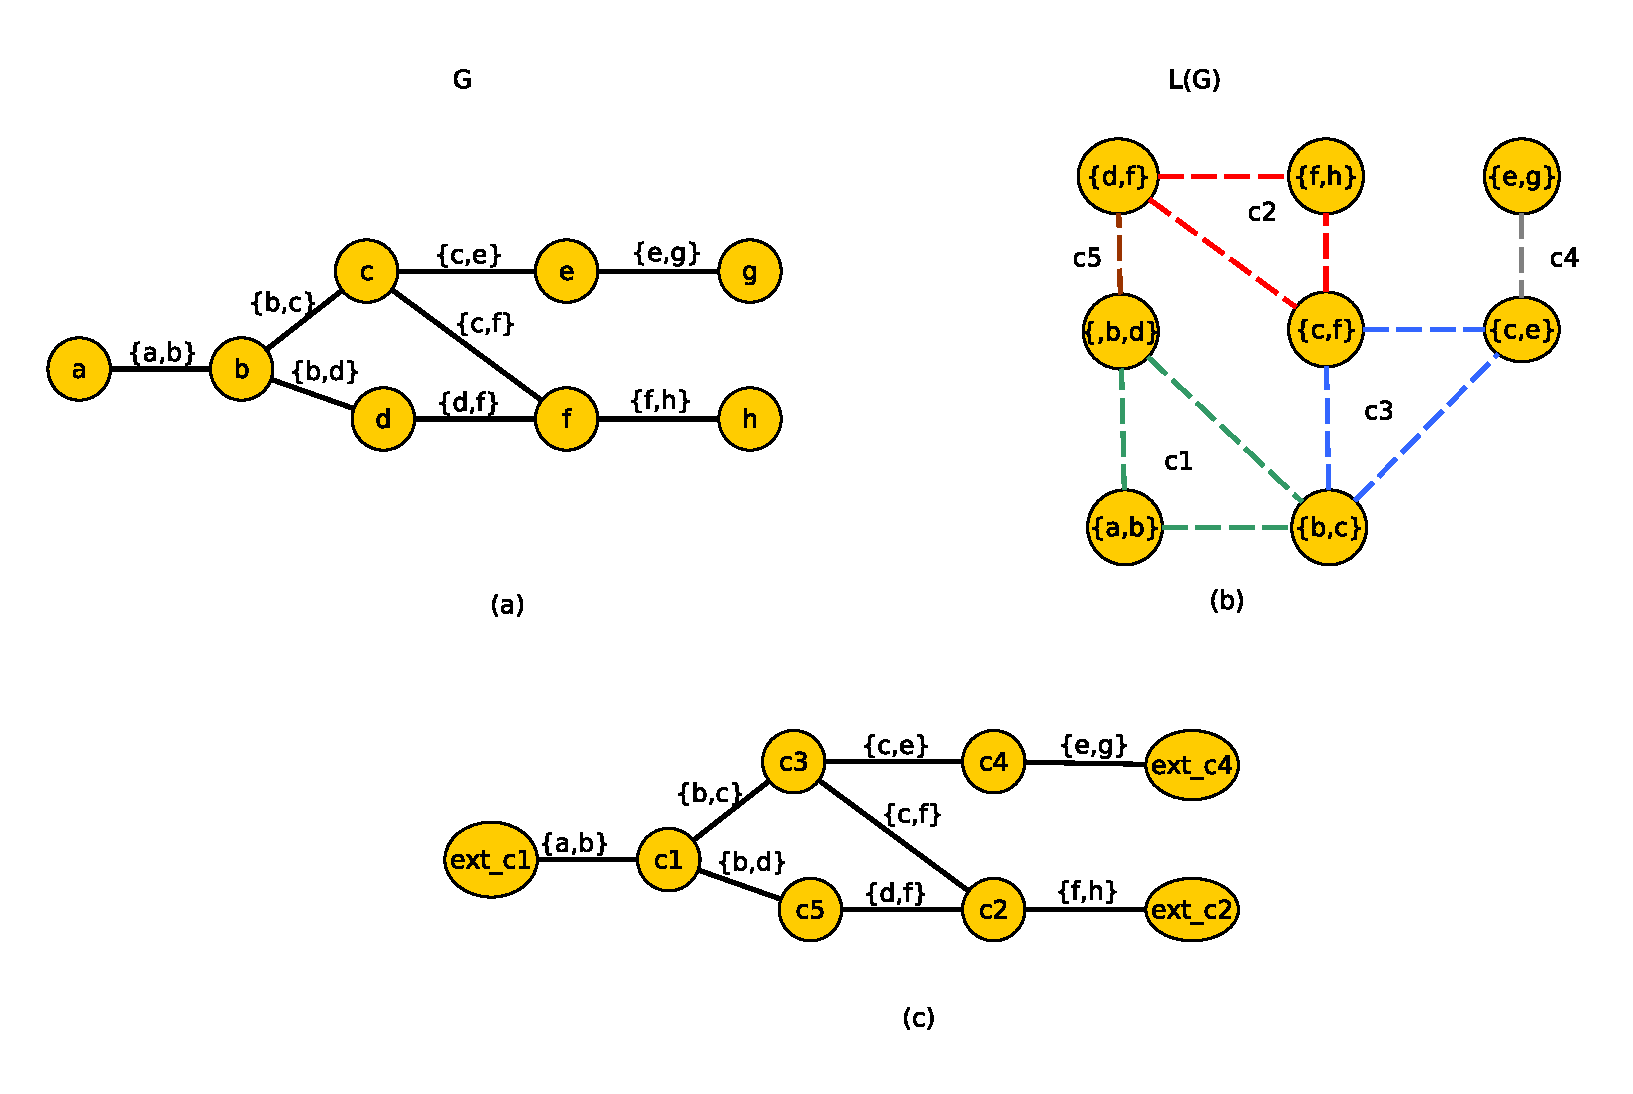
\includegraphics[scale = 0.7]{ExempleGraphesRacinesIsomorphes.eps}
\caption{ Construction de la topologie non orient\'e de $G_c$.
		(a) : r\'eseau initial mod\'elis\'e par $G$.
		(b) : line graphe de $G$.
		(c) : graphe $G'$ reconstruit.
		 }
\label{ExempleGraphesRacinesIsomorphes}
\end{figure}
%\FloatBarrier
% ---- figure exemple correction graphe cellule G_{3,3}

\subsection{Orientation du graphe $G'$}
Nous supposons que le graphe non orient\'e $G'=(V',E')$ sous-jacent au DAG $G$ a d\'ej\`a \'et\'e  obtenu. Nous orientons les ar\^etes de $G'$ afin de d\'ecouvrir  le DAG cible.
 \newline
 
 Soient 
 un sommet $v$, 
 son voisinage $N(v)$ et 
 une bipartition $p(v)$, $s(v)$ de $v$.
 \newline
 Si $Verif-correl (p(v), s(v)) = 1$ alors la partie $p(v)$ est l'ensemble $p(v)$ des arcs entrants de $v$ et  la partie $s(v)$ est l'ensemble $s(v)$ des arcs sortants de $v$.    
Sinon la bipartition n'est pas la bonne et nous testons une autre bipartition.
Nous testons ainsi dans l'ordre de $2^{d(v)}$ bipartitions avec $d(v) = |N(v)|$ dans le pire des cas,.
\newline
Soit une s\'equence $S = v_1, v_2, \cdots, v_k$ de sommets de $G$ telle que 
chaque ar\^ete est incidente \`a $\{v_1, \cdots, v_k\}$ et que  $\{v_1, \cdots, v_{k-1}\}$ n'a pas cette propri\'et\'e.
\newline
Soit $d_i$ le nombre d'ar\^etes liant $v_i$ \`a un sommet  de $V-\{v_1,\cdots, v_{i-1}\}$.
%On determine la couverture. {\bf bizarre} 
\newline
Nous allons prendre dans l'ordre chaque sommet de la s\'equence $S$ et nous allons traiter ses ar\^etes pour trouver une bipartition correcte.
Si une ar\^ete a d\'ej\`a \'et\'e trait\'ee pour un sommet, elle n'est plus prise en compte dans les ar\^etes incidentes des sommets suivants dans la s\'equence $S$.
Le traitement du sommet $v_i$ n\'ecessite $2^{d_i}$ op\'erations et le nombre total d'op\'erations est alors 
$$
 2^{d_1} + 2^{d_2} + \cdots + 2^{d_k}
$$  
Notre probl\`eme  est de trouver une telle liste telle que cette somme est minimum.
L'heuristique est, \`a chaque \'etape, de choisir le sommet tel que 
le nombre d'ar\^etes incidentes non encore trait\'ees est minimum.
Par exemple, on commence par le sommet $v_1$ comme sommet de degr\'ee minimum. 
\`A chaque \'etape, on prend le sommet $v_i$ tel que son degr\'e $d_{v_i}$ est minimum.
\newline 

\vspace{-0.5cm}
Cependant, cette heuristique n'est pas optimale et voici un contre-exemple illustr\'e par la figure \ref{orientationAretesHeuristiqueContreExemple}. \newline
Soit le graphe $H$ compos\'e de $3$ cliques $K_5$ et d'un sommet $v$ ayant une ar\^ete incidente avec un seul sommet dans chaque clique $K_5$.
Le sommet $v$ est de degr\'e minimum. 
Nous consid\'erons $2$ s\'equences de sommets diff\'erents pour d\'enombrer les bipartitions. 
La premi\`ere s\'equence suit l'heuristique et la seconde s\'equence d\'ebute par un sommet de $K_5$ de degr\'e $4$. 
\newline
Soit $c(S)$ la somme des bipartitions possibles.  
En consid\'erant l'heuristique, nous d\'ebutons par $v$. 
Puis le sommet suivant de degr\'e minimum est un sommet de $K_5$. On traite tous les sommets de cette clique $K_5$ avant de passer \`a une autre clique $K_5$.
Le nombre de bipartitions trait\'ees avec  l'heuristique est 
$$
	c(S_H) = 2^3 + 3(  2^4 + 2^3+ 2^2 +2^1) = 98
$$
En consid\'erant la seconde s\'equence, on choisit le sommet de $K_5$ de degr\'e minimum. On traite ce sommet en $2^4$ bipartitions. Le sommet suivant est encore dans cette clique mais le nombre de bipartitions baisse \`a $2^3$.
Apr\`es les deux sommets trait\'es, le nombre de bipartitions est $2^4+2^3$.
On r\'ep\`ete le traitement des sommets jusqu'\`a ce que tous les sommets soient trait\'es avant de passer \`a une autre clique $K_5$. 
Dans cette clique, on reprend \`a nouveau la seconde s\'equence.
Le nombre de bipartitions  trait\'ees avec la seconde s\'equence est 
$$
	c(S_2) = 3(  2^4 + 2^3+ 2^2 +2^1) = 96
$$
Nous remarquons que le nombre de bipartitions avec la seconde s\'equence est minimum.
Cet exemple confirme que la solution de l'heuristique n'est pas minimale car il existe une autre s\'equence de choix de ces sommets (ici la seconde  s\'equence) qui minimise le nombre de bipartitions. 
% ---- figure contre exemple  heuristique orientation aretes 
\begin{figure}[htb!] 
\centering
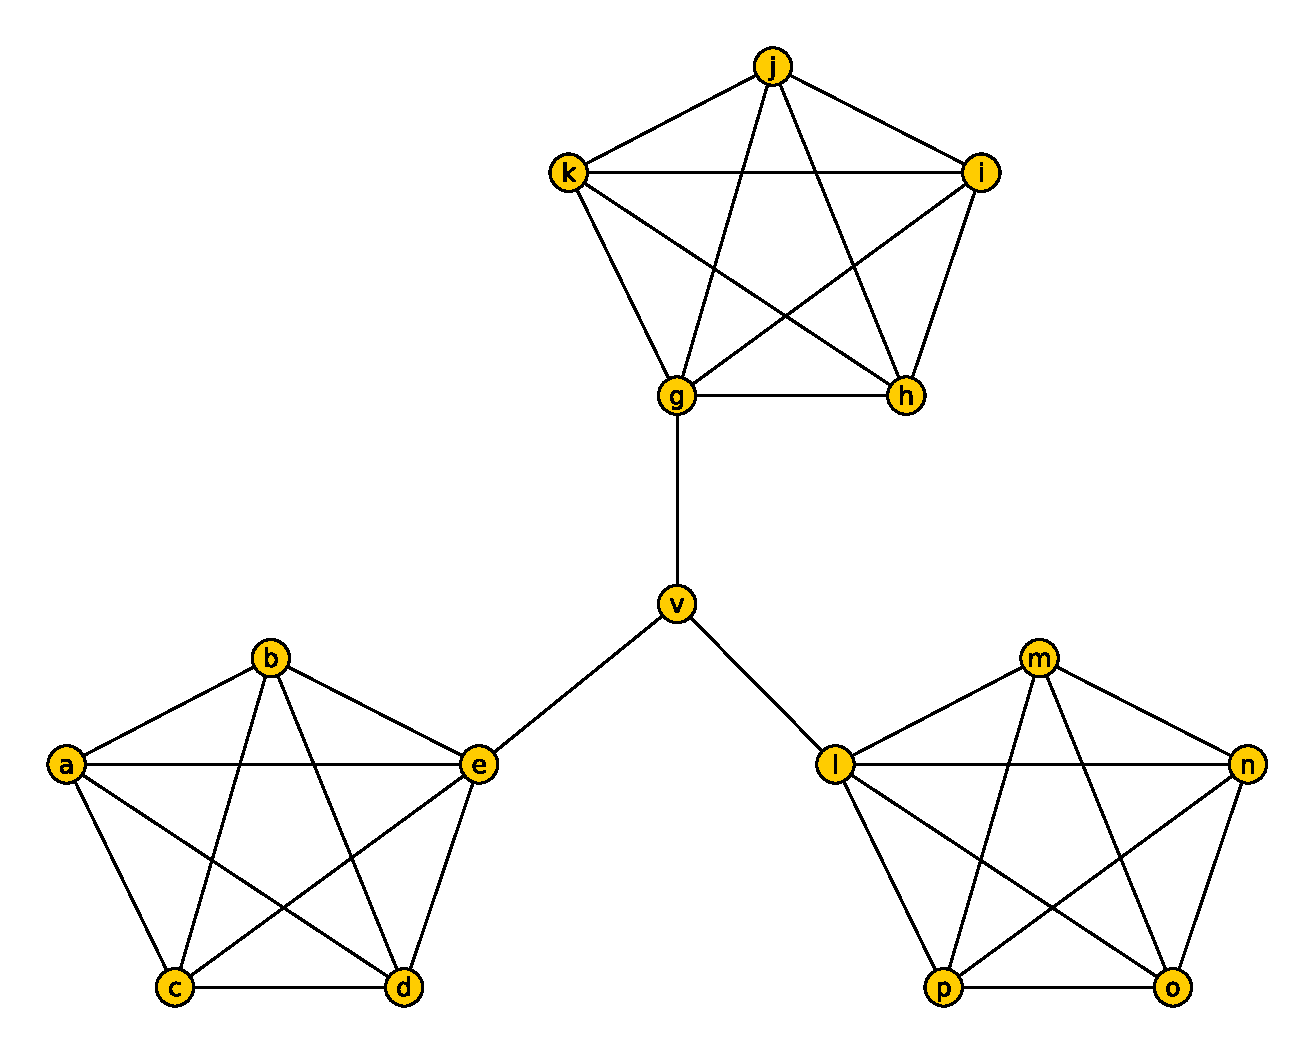
\includegraphics[scale = 0.7]{orientationAretesHeuristiqueContreExemple.eps}
\caption{ Un contre-exemple de l'heuristique choisie pour l'orientation des ar\^etes.
		 On choisit un sommet de degr\'e minimum dans une clique $k_5$. Ensuite, on traite tous les sommets de la clique et on se sert du degr\'e minimum pour choisir les sommets de la s\'equence. Puis on passe \`a une clique et on reprend le traitement jusqu'\`a ce qu'il ne reste plus d'ar\^etes dans une seule clique.
		}
\label{orientationAretesHeuristiqueContreExemple}
\end{figure}
\FloatBarrier
% ---- figure contre exemple  heuristique orientation aretes
%\newline

{\bf Conclusion} : 
l'algorithme d'orientation que nous avons propos\'e choisit le sommet de degr\'e minimum \`a chaque \'etape de l'algorithme et cette solution n'est pas optimale.
Nous conjecturons que la s\'equence $S$ de traitement des sommets est $NP-complet$.


%On le traite avec  $2^3$ bipartitions. Ensuite le sommet suivant de degr\'e minimum est un sommet de $K_5$. On le traite en $2^4$ bipartitions      
%
%
%
%
%Nous supposons que le graphe non-orient\'e $G'=(V',E')$ sous-jacent au DAG $G_c$ ait d\'ej\`a \'et\'e construite. Nous orientons les ar\^etes de $G'$ afin qu'il soit un DAG.
% \newline
% 
%Soit $O = (v_1,v_2, \cdots, v_n)$ la s\'equence de traitement des sommets de $G'$ tel que 
%$d_1 \le d_2 \le \cdots \le d_n$ avec 
%$d_i$ le degr\'e du sommet $v_i$. $d_i$ est aussi le le nombre d'ar\^etes incidentes \`a $v_i$ non trait\'es.
%\newline
%Consid\'erons le premier sommet $v_1$ \`a traiter de $O$ et $N(v_1)$ l'ensemble des  ar\^etes incidentes \`a $v_1$.
%Nous subdivisons $N(v_1)$ en $2$ partitions telles que 
%\begin{itemize}
%	\item $pred(v_1)$ est l'ensemble des ar\^etes pr\'ed\'ecesseurs \`a $v_1$.
%	\item $succ(v_1)$  est l'ensemble des ar\^etes successeurs \`a $v_1$.
%\end{itemize}
%Nous testons cette bipartition $(pred(v_1), succ(v_1))$ avec la fonction $Verif-correl$ \ref{VerifCorrel}.
%Si $Verif-correl$ retourne $Vrai$ alors nous avons orient\'e les ar\^etes incidentes \`a $v_1$.
%Sinon nous testons une autre bipartition.
%Dans le pire des cas, nous testons $2^{d_1}$ bipartitions pour trouver la bonne.
%\newline
%Soit  $(pred(v_1), succ(v_1))$ la bonne bipartition de $v_1$.
%\'Etant donn\'ee que $G'$ est un graphe connexe et que une ar\^ete $a_i$ est form\'ee par les sommets $v_i$ et $v_j$ de $G'$, 
%$a_i$ appartient \`a l'ensemble des successeurs de $v_j$ si $a_i$ a d\'ej\`a \'et\'e trait\'e en pr\'ed\'ecesseur de $v_i$.
%De m\^eme, $a_i$ appartient \`a l'ensemble des pr\'ed\'ecesseurs de $v_j$ si $a_i$ a d\'ej\`a \'et\'e trait\'e en successeur de $v_i$.
%Ainsi, le nombre de bipartitions \`a tester devient moins important au traitement d'un nouveau sommet de $O$.
%En effet, le nombre de bipartitions \`a tester en traitant le sommet  $v_2$ est $2^{d_2}$ et $2^{d_2} \le 2^{d_1}$.
%En traitant le dernier sommet $v_n$ de $O$, nous testons une seule bipartition parce que tous les ar\^etes ont d\'ej\`a \'et\'e trait\'es. Cette bipartition est la bonne et $2^{d_n} = 1$.
%\newline
%Nous d\'eduisons que 
%$$
%1 = 2^{d_n} \le \cdots \le 2^{d_2} \le 2^{d_1}
%$$
%
%L'algorithme d'orientation que nous avons propos\'e choisit le sommet de degr\'e minimum \`a chaque \'etape de l'algorithme et cette solution est minimale.
%Nous conjecturons que la s\'equence $O$ de traitement des sommets est $NP-complet$.
%
%
%
%%% ----
%%% decouverte de topologie du reseau energetique
%%% ----
%%Soient $\cal H$, l'ensemble des cliques de la line-graphe $G_c$ et $G$ le graphe racine de $G_c$. \newline
%%Chaque clique $C_k \in {\cal H}$ correspond \`a un sommet du graphe racine $G$. \newline 
%%Soit $u = \{ENTRANT, SORTANT, NONE\}$, l'ensemble des marquages de chaque ar\^ete tel que les \'etiquettes {\em ENTRANT} et {\em SORTANT} sont associ\'ees respectivement \`a l'ar\^ete $a_i$ entrante et \`a l'ar\^ete $a_j$ sortante du sommet $C_k$.
%%\newline
%%%-- definition de S_1 e S_2
%%Soient $S_1$ et $S_2$ l'ensemble des arcs entrants et sortantes du sommet $C_k$.
%%\begin{equation}
%%S_\alpha = \{ S_{\alpha,i}, \hspace{0.2 em} \forall i \le 2^{card(C_k)+1}  \}
%%\end{equation}
%%avec $i$, le nombre de sous-ensemble de $C_k$ et $\alpha = \{1,2\}$. Le sous-ensemble $S_{\alpha,i}$ peut \^etre  l'ensemble vide $\emptyset$.
%% 
%% %--  ORACLE ou Verif-correl
%% \begin{definition}
%% Soit la clique $C_k$ de la line-couverture {\cal H}.
%% Un couple $(S_1,S_2)$ de sous-ensembles de $C_k$ est {\bf valide} si 
%% \begin{itemize}
%% \item $S_1 \ne S_2$
%% \item $S_1 \cup S_2 = C_k$
%% \item $S_1 \cap S_2 = \emptyset$
%% \end{itemize}
%% \end{definition}
%% 
%% \begin{definition}
%% Soit une fonction bool\'eenne $Verif-correl$ d\'efinit de $S_1 \times S_2 \rightarrow \{0,1\}$, avec le couple valide $(S_1,S_2)$.
%% La fonction $Verif-correl$ renvoie $1$ si et seulement si la loi de conservation autour du sommet $C_k \in G$ est respect\'ee c'est-\`a-dire : 
%% \begin{equation}
%% \forall a_i \in S_1, \forall a_j \in S_2, \sum_{a_i \in S_1} gp_{a_i} - \sum_{a_j \in S_2} gp_{a_j} \le \epsilon
%% \end{equation}
%% avec $\epsilon$ les pertes minimales par effets joules, $gp_{a_i}$ le flot dans l'arc $a_i \in E(G_c)$.
%% \end{definition}
%% 
%% \begin{property}
%% Si $Verif-correl(S_1, S_2) = 1$ alors l'ensemble  $S_1$ est l'ensemble des arcs entrants et  $S_2$ l'ensemble des arcs sortants du sommet $C_k \in G$.
%% \end{property} 
%%Les arcs de $S_1$ et $S_2$ ne concourent pas \`a un sommet $C_k$ lorsque  $Verif-correl(S_1, S_2) = 0$.
%%
%%\begin{theorem}
%%\label{arcsentrantsSortants}
%%%Un arc $a_i$ est soit {\em entrant}, soit {\em sortant} mais jamais les deux.
%%Si un sommet $a_i \in G_c$ appartient \`a deux cliques $C_{k_1}, C_{k_2} \in {\cal H}$ alors 
%%l'arc  $a_i \in E(G_c)$ est soit {\em entrant} de $C_{k_1}$  et {\em sortant} de $C_{k_2}$ ou soit {\em entrant} de $C_{k_2}$  et {\em sortant} de $C_{k_1}$.
%%\end{theorem}
%%
%%\begin{proof}
%%D'apr\`es le th\'eor\^eme \ref{caracteristiquesLinegraphes}, le sommet $a_i$ appartient \`a deux cliques $C_{k_1}$ et $C_{k_2}$ au maximum. 
%%Cela implique qu'il existe une ar\^ete entre les sommets $C_{k_1}$ et $C_{k_2}$ dans $G$.
%%Soient $S_1, S_2 \subset C_{k_1}$ et $S_3, S_4 \subset C_{k_2}$ telles que $Verif-correl(S_1, S_2) = 1$ et $Verif-correl(S_3, S_4) = 1$.
%%Comme  $S_1 \cap S_2 = \emptyset$, $S_3 \cap S_4 = \emptyset$ et aussi  $C_{k_1} \cap C_{k_2} = \{a_i\}$, on a quatre choix possibles :
%%$a_i \in S_1 \cap S_3$, $a_i \in S_1 \cap S_4$, $a_i \in S_2 \cap S_3$, $a_i \in S_2 \cap S_4$.
%%\newline
%%Si $a_i$ est entrant \`a $C_{k_1}$ et sortant \`a  $C_{k_2}$ alors $a_i \in S_1 \cap S_3$ ou  $a_i \in S_2 \cap S_4$. 
%%On en d\'eduit qu'il existe une boucle sur le sommet $C_{k_1}$ et $C_{k_2}$. 
%%Cela est impossible parce que $G$ est un $DAG$. 
%%\newline
%%Ainsi si $a_i$ est entrant \`a $C_{k_1}$ alors $a_i \in S_2 \cap S_3$ ou  si $a_i$ sortant \`a $C_{k_2}$  alors $a_i \in S_1 \cap S_4$. 
%%\end{proof}
%%
%%consid\'erons l'ensemble $A$ des cliques $C_j$ tel que $card(C_j) = min\{ card(C_k), C_k \in {\cal H}\}$ et la fonction  $Z$ qui retourne l'\'etiquette d'un sommet dans une clique. $Z$ est d\'efinie comme suit:
%%$E \times {\cal H} \rightarrow \{ENTRANT, SORTANT, NONE\} $.
%%\newline
%%Soit la fonction $f$ d\'efinie sur $ V(G_c) \times A \rightarrow \{0,1\}$ retournant $1$ si le sommet $a_i^u$ ne poss\`ede aucune \'etiquette c'est-\`a-dire labellis\'e \`a $None$.
%%$$ f(a_i^u, C_j) = \begin{cases} 1 ~~~ si ~~~ Z(a_i^u, C_j) \ne NONE \\ 0 ~~~ sinon \end{cases}$$.
%%La fonction $MA$ calcule le nombre de sommets labellis\'e dans une clique $C_k$.
%%$$MA(C_k) =  \sum_{a_i^u \in C_k} f(a_i^u,C_k) $$
%%Soient la clique $C_m$ telle que  $MA(C_m) = max\{ MA(C_j), C_j \in A\}$ et $B$ l'ensemble des sommets de la clique $C_m$ tel que $Z( a_j^v, C_m) == NONE, ~ \forall ~ a_j^v \in B$. 
%%
%%
%%%nommer l'algorithme
%%\begin{algorithm}[!ht]
%%\caption{Decouverte\_graphe\_racine}
%%\noindent DEBUT\\
%%\noindent 1. Initialisation des \'etiquettes des sommets $a_i$ de $G_c$, et $C_k \in {\cal H}$ \\
%%\noindent $Z( C_k, a_i^u) = None$ \\
%%~2. \indent {\bf Tant que} il existe une  ar\^ete de $G_c$ ($E(G_c)$) \\
%%	\indent~~~~~~{\bf Faire}\\
%%~3.		\indent~~~~~~~~choisir $A = \{C_j , card(C_j) = min\{ card(C_k), C_k \in {\cal H} \}\}$ \\
%%~4.		\indent~~~~~~~~choisir $C_k$ tel que $MA(C_k) = max\{ MA(C_j), C_j \in A\} $ \\
%%~5.       	\indent~~~~~~~~{\bf Si} il existe $S_1$ et $S_2$ tel que $S_1 \cap S_2 = \emptyset $ et $S_1 \cup S_2 = C_k $ et $Verif-correl(S_1, S_2 )= 1 $ \\
%%~6.	       	\indent~~~~~~~~~~~~{\bf alors}\\
%%~7.	       	\indent~~~~~~~~~~~~ $S_1^k = sommets\_marques(S_1, Z)(^1)$; \\
%%~8.	       	\indent~~~~~~~~~~~~ $S_2^k = sommets\_marques(S_2, Z)$; \\
%%~9.		\indent ~~~~~~~~~~~~{\bf Pour tout} $a_i^K \in S_1 - S_1^k$ {\bf Faire} \\
%%~10.		\indent ~~~~~~~~~~~~~ $Z(C_k, a_i^K) = ENTRANT$ \\
%%~11.		\indent ~~~~~~~~~~ {\bf Pour tout} $a_i^K \in S_2 - S_2^k$ {\bf Faire} \\
%%~12.		\indent ~~~~~~~~~~~~~ $Z(C_k, a_i^K) = SORTANT$ \\
%%~13.		\indent~~~~~~~~~~ $E(G_{c}) =  E(G_c)  - E(G_c[C_k])$ \\
%%~14.		\indent~~~~~~~~~~ ${\cal H} =  {\cal H}  - C_k$ \\
%%~15.       	\indent~~~~~~~~{\bf FinSi} \\
%%~16. \indent {\bf FinTant que} \\
%%~17. \indent {\bf Pour tout} $a_i^u \in V(G_c)$ {\bf Faire} \\
%%~18. \indent ~~~ $C_1, C_2$ = $Couverture\_Cliques(a_i^u)(^2)$\\
%%~19. \indent ~~~ {\bf Si } $C_1 \neq \emptyset$ et $C_2 \neq \emptyset$ {\bf Alors} \\
%%~20. \indent ~~~~~~  {\bf Si}  $Z(C_1, a_i^u) == SORTANT$ {\bf Alors} \\
%%~21. \indent ~~~~~~~~~~~~ $Mat(C_1)$ += $C_2$ $(^3)$ \\  
%%~22. \indent ~~~~~~  {\bf Fin Si} \\
%%~23. \indent ~~~~~~  {\bf Si}  $Z(C_2, a_i^u) == SORTANT$ {\bf Alors} \\
%%~24. \indent ~~~~~~~~~~~~ $Mat(C_2)$ += $C_1$ $(^3)$ \\  
%%~25. \indent ~~~~~~  {\bf Fin Si} \\
%%~26. \indent ~~~ {\bf Fin si} \\
%%~27. \indent ~~~ {\bf Si } $C_1 \neq \emptyset$ et $C_2 == \emptyset$ {\bf Alors} \\
%%~28. \indent ~~~~~~  {\bf Si}  $Z(C_1, a_i^u) == ENTRANT$ {\bf Alors} \\
%%~29. \indent ~~~~~~~~~~~~ $Mat(EXT\_a_i^u)$ += $C1$ $(^3)$\\  
%%~30. \indent ~~~~~~  {\bf Fin Si} \\
%%~31. \indent ~~~~~~  {\bf Si}  $Z(C_1, a_i^u) == SORTANT$ {\bf Alors} \\
%%~32. \indent ~~~~~~~~~~~~ $Mat(C_1)$ += $EXT\_a_i^u$ $(^3)$ \\  
%%~33. \indent ~~~~~~  {\bf Fin Si} \\
%%~34. \indent ~~~ {\bf Fin si} \\
%%~35. \indent {\bf Fin Pour} \\
%%~36. \noindent {\bf Return} Mat\\
%%\noindent FIN\\
%%\end{algorithm}
%%
%%\FloatBarrier
%%$^1$ : Cette fonction retourne les sommets de l'ensemble $S_1$ labellis\'es \`a $ENTRANT$ et $S_2$ labellis\'es \`a $SORTANT$. Initialement, Ces sommets sont \'etiquett\'es \`a $NONE$.
%%
%%$^2$ : Cette fonction renvoie les cliques couvrantes une ar\^ete $a_i^u$ avec $C_1 \ne \emptyset$. Si $a_i^u$ est couvert par une clique alors $C_2 = \emptyset$.
%%
%%$^3$ : $EXT\_a_i^u$ est un sommet du graphe racine $G$.
%%\newline
%%
%%L'algorithme {\em Decouverte\_graphe\_racine} d\'ebute par l'initialisation des sommets de $G_c$ \`a $''None''$.
%%Tant qu'il existe une ar\^ete dans notre line-graphe $G_c$, on choisit la plus petite clique $C_k$ dans laquelle le nombre de sommets labellis\'es est maximal quelque soit le label {\em ENTRANT} et {\em SORTANT} (lignes $3-4$).
%%On partitionne la clique $C_k$  en deux sous-ensembles valides $S_1$ et $S_2$ tels que $S_1$ et $S_2$ correspondent, respectivement, \`a l'ensemble des arcs entrants et sortants du graphe racine $G$.
%%Les sommets labellis\'es de $S_1$ not\'es $S_1^k$ portent l'\'etiquette $ENTRANT$ tandis que ceux labellis\'es en $''SORTANT''$ sont not\'es $S_2^k$ (lignes $6-12$). 
%%Ensuite nous mettons \`a jour l'ensemble des ar\^etes et la line-couverture  $\cal C$ de $G_c$ (lignes $13-14$). 
%%\newline
%%Une fois termin\'e l'orientation des ar\^etes de $G$ qui  sont les sommets labellis\'es du line-graphe $G_c$ (lignes $2-16$), nous construisons la liste d'adjacence de chaque sommet de $G$ (lignes $17-36$).
%%Nous recherchons la couverture d'un sommet $a_i^u$ de $G_c$.
%%\newline 
%%Si le sommet  $a_i^u$ est couvert par une seule clique alors $C_2 = \emptyset$. Dans ce cas, cela signifie qu'il existe un arc entre le sommet $C_1$ et le sommet $EXT\_a_i^u$ que nous avons cr\'ee. Cet arc a pour extr\'emit\'e initiale $C_1$ si $a_i^u$ est labellis\'e par $SORTANT$ sinon pour extr\'emit\'e initiale $EXT\_a_i^u$ si $a_i^u$ est labellis\'e par $ENTRANT$ (lignes $27-34$).
%%\newline
%%Dans le cas o\`u le sommet $a_i^u$ est couvert par deux cliques non vides $C_1, C_2$, nous ajoutons un arc entre ces deux cliques.
%%D'apr\'es le th\'eor\`eme  \ref{arcsentrantsSortants}, nous d\'efinissons  $C_1$ comme extr\'emit\'e initiale de cet arc si $a_i^u$ est labellis\'e par $SORTANT$ dans cette clique $C_1$. Dans le cas o\`u $a_i^u$ est labellis\'e par $SORTANT$ dans cette clique $C_2$, $C_2$ est l'extr\'emit\'e finale de cet arc (lignes $19-26$).
%%%D'apr\'es le th\'eor\`eme  \ref{arcsentrantsSortants} stipulant qu'un sommet de $G_C$ est $''ENTRANT''$ de $C_1$ et $''SORTANT''$ de $C_2$ et vice-versa, nous d\'efinissons  $C_1$ comme extr\'emit\'e initiale de cet arc si $a_i^u$ est labellis\'e par $SORTANT$ dans cette clique $C_1$ sinon $C_2$ si $a_i^u$ est labellis\'e par $SORTANT$ dans cette clique $C_2$ (lignes $19-26$).
%%
%%\subsection{Complexit\'e de l'algorithme {\em Decouverte\_graphe\_racine} }
%%
%%La fonction $Couverture\_Cliques$ a une complexit\'e constante $O(1)$ alors que la complexit\'e de la  fonction $sommets\_marques$ depend du nombre de sommets dans $S_1$. Dans le pire des cas, sa complexit\'e est $O(n)$ avec $n = E(G)$ le nombre  d'arcs de $G$. Donc les lignes $17-35$ s'ex\'ecutent en $O(n)$ dans le pire des cas. 
%%\newline
%%Consid\'erons une line-couverture ${\cal H}$  de taille $K$,  une clique $C_i \in {\cal H}$ de taille $p_i$ et $k_i$ le nombre de sommets marqu\'es dans $C_i$. 
%%\newline
%%Le nombre de couples valides $(S_1,S_2)$ pour la clique $C_i$ avec $k_i$ sommets marqu\'es est $2^{p_i -k_i}$. 
%%Au traitement de la premi\`ere clique de ${\cal C}$ de taille minimale $C_1$, il existe $0$ sommet marqu\'e. Le co\^ut $R_{cv_1}$ de couples valides est $R_{cv_1} = 2^{p_1}$.
%%Au traitement de la seconde clique $C_2$, il existe $k_2 \ge 0$ et son co\^ut est  $R_{cv_2} = 2^{p_2 - k_2}$.
%%Il existe une clique $C_\alpha$ \`a partir de laquelle $k_\alpha > 0, \alpha \le K$.
%%On remarque que $p_\alpha - k_\alpha$ est d\'ecroissant car $k_\alpha$ augmente apr\`es chaque traitement de cliques. 
%%Cela signifie qu'\`a la selection de la derni\`ere clique $C_k$, son co\^ut  est de $R_{cv_K} = 1$. 
%%Le co\^ut est decroissant \`a chaque traitement c'est-\`a-dire 
%%$$2^{p_{\alpha} - k_{\alpha}} \ge 2^{p_{\alpha+1} - k_{\alpha+1}} \ge \cdots \ge 2^{p_K - k_K}$$ 
%%Le co\^ut des couples valides de ${\cal H}$ est 
%%$$R_{cv} = O(2^\gamma), \gamma = max\{card(C_i), \forall C_i  \in \{C_1, \cdots, C_\alpha\} \}$$
%%car il depend de la clique $C_i \in \{C_1, \cdots, C_\alpha\} \subset {\cal H}$.
%%\newline
%%Le co\^ut des lignes $3-4$ depend de $p_i$ et $K$ ($O(p_i) + O(K)$) et celui des lignes $7-14$ est de $O(p_i^2)$.
%%\newline
%%Soit le co\^ut $R$ de la boucle  {\em Tant que}. Il est de 
%%$$ R = O(p_i) + O(K) + O(p_i^2) + O(2^\gamma) \simeq O(2^\gamma)$$
%%
%%La complexit\'e de {\em Decouverte\_graphe\_racine} est {\em pseudo-exponentielle} car l'exposant $\gamma$ est la taille d'une clique de taille interm\'ediaire.
%%
%%%Consid\'erons les instructions dans le boucle {\em Tant que}, $K$ le cardinal de ${\cal C}$ et $p$ le cardinal de la clique de taille minimale de ${\cal C}$ c'est-\`a-dire $card(A) = p$. 
%%%\newline
%%%$R_i$ est le co\^ut de la boucle {\em Tant que} au traitement de la $i^eme$ clique de $G_C$ et $C\_oracle$ le co\^ut de la fonction $ORACLE$.
%%%S\'electionnons le premier clique de $G_C$. Son co\^ut est :
%%%$$R_1 = p \times C_oracle(S_{1p}, S_{2p}) $$.
%%%Le co\^ut  du deuxi\`eme sommet est :
%%%$$R_2 = p \times C_oracle(S_{1p}, S_{2p})  + (p-1) \times C_oracle(S_{1p-1}, S_{2p-1})  $$.
%%%Le co\^ut des $n$ sommets de $G_C$ est :
%%%$$R_K = \sum_{k = 0}^{K-1} (p-k) \times C_oracle(S_{1p-k}, S_{2p-k})$$
%%%
%%%La particularit\'e de l'ORACLE est que pour $k \ge p$, tous les sommets de la clique $C_k$ sont labellis\'es entrainant qu'on ne genere aucuns sous-ensembles de $C_k$. Cela implique que  $C_oracle(S_{1p-k}, S_{2p-k}) = 1$. \newline
%%%Cela revient \`a dire que le co\^ut $R_K$ est d\'ecroissant en fonction de $K$. \newline
%%%G\'en\'erer tous  sous-ensembles de $C_k$ de taille $p$ est une combinaison de 
%%%$card(P(E)) = 2^{p}$ et toutes les paires de $P(E)$ vaut au pire des cas $\frac{2^p * (2^p - 1)}{2}$. 
%%%Alors  le  cout  $C_oracle(S_{1p}, S_{2p}$ est $O(2^p)$ ===> FAUX
%%%%%%% A discuter avec SERGES ---> trouver le nombre de tuples provenant des sous ensembles  de C_k de taille $p$
%%%Donc le co\^ut de $R_K$ est  
%%%$$R_K = p \times O(2^p) + (p-1) \times O(2^{(p-1)}) + \cdots + 1 \times O(2^0)$$
%%%$$ R_K $$
%%%PAS FINI
%%
%%

		
%--------------------------------------------------------------------
%------- 	conclusion chapitre		 ---------------------
%--------------------------------------------------------------------
%\section{Conclusion du chapitre \ref{linegraphesChapitre} }
\section{Conclusion du chapitre 4 }
	%%% reformulation et correction 
Nous avons d\'ecrit la relation existante entre la matrice de corr\'elation et la notion de line-graphe. En effet, la matrice de corr\'elation appliqu\'ee \`a une valeur de seuil est la matrice d'adjacence d'un line-graphe si elle ne contient aucune erreur de corr\'elation.  Dans le cas o\`u elle poss\`ede des cases \'erron\'ees, il est impossible de d\'eterminer la {\em couverture de corr\'elation} du graphe de corr\'elation. Nous avons alors d\'efini le probl\`eme {\em Proxi-Line} dont l'objectif est de trouver le line-graphe  qui a le moins d'ar\^etes diff\'erentes avec le graphe de corr\'elation.  
\newline

Ensuite, nous avons pr\'esent\'e les propri\'et\'es d'un line-graphe et les travaux existants dans la d\'ecouverte de couverture en cliques sur des line-graphes. Nous avons retenu l'algorithme de Lehot \cite{decompositionEnCliques} comme la base de notre algorithme de couverture parce qu'il attribue  des \'etats \`a tous les sommets \`a chaque \'etape de l'algorithme. Cette op\'eration permet de connaitre les sommets non couverts des sommets d\'ej\`a couverts. 
\newline
Dans le but de r\'esoudre le probl\`eme {\em Proxi-Line}, nous proposons ainsi deux algorithmes. 
\newline
Le premier algorithme est {\em l'algorithme de couverture} et il couvre tous les sommets par une ou deux cliques \`a partir des \'etats des sommets. Nous avons distingu\'e trois types d'\'etats.
En effet, un sommet couvert par une clique et qui poss\`ede des ar\^etes incidentes est \`a l'\'etat  $2$. Un sommet couvert par une clique ou deux cliques et qui n'a aucune ar\^ete incidente est \`a l'\'etat $1$. Un sommet couvert par deux cliques ayant des ar\^etes incidentes ou un sommet ayant des ar\^etes incidentes qui ne forment pas une clique est \`a l'\'etat $-1$. 
L'ensemble des sommets $v$ \`a l'\'etat $-1$ est l'ensemble $\cal C$ de sommets \`a corriger. \`A la fin de l'algorithme, il retourne les cliques d\'ecouvertes (couverture de corr\'elation $\cal CC$). 
\newline
Le second algorithme propos\'e est {\em l'algorithme de correction}. Il se base sur l'ensemble $\cal C$ et les cliques d\'ecouvertes pendant l'algorithme de couverture. 
En effet, cet algorithme s\'electionne chaque sommet $u \in \cal C$ et le corrige en proc\'edant par une phase d'augmentation et de compression.
La phase d'augmentation d\'etermine les cliques de $\cal CC$ contenant $u$, les cliques de $\cal CC$  dont $u$ partage une ar\^ete avec un sommet de la clique (cliques voisines), les cliques contractables (cliques de $\cal CC$ dont l'intersection retourne le sommet $u$) et les cliques d\'ependantes (cliques contenant $u$ dans lesquelles un des sommets partagent une ar\^ete avec une clique de la couverture  de corr\'elation $\cal CC$). 
Puis elle effectue le produit cart\'esien de ces ensembles de cliques. Chaque \'el\'ement de ce produit est not\'e $\pi_1$ ou $\pi_2$.
Quant \`a la phase de compression, elle s\'electionne deux \'el\'ements du produit cart\'esien qu'elle note  $\pi_1$ et $\pi_2$, puis elle ajoute des ar\^etes de  $\pi_1$ et $\pi_2$ dans l'ensemble des ar\^etes initiales du graphe de correction pour en faire des cliques. Elle cr\'ee aussi l'ensemble $\pi_s$ des ar\^etes \`a supprimer afin que le sommet $u$ ne soit couvert que par deux cliques. 
Les cliques $\pi_1$ et $\pi_2$ sont ajout\'ees \`a la couverture de corr\'elation $\cal CC$. 
La complexit\'e des algorithmes de couverture et de correction est {\em pseudo-polynomiale} en fonction du degr\'e du graphe de corr\'elation. 
\newline 

Enfin, la derni\`ere section pr\'esente la construction de la topologie du graphe racine et son orientation. Pour la construction de la topologie, nous nous servons principalement de la couverture de corr\'elation. En effet, chaque clique de cette couverture de corr\'elation est un sommet dans le graphe racine. Si l'intersection de deux cliques est non vide alors il existe une ar\^ete entre les sommets correspondant \`a ces cliques dans le graphe racine. 
Concernant l'orientation des ar\^etes, nous nous servons de la fonction $Verif-correl$ (section \ref{VerifCorrel}) qui teste tous les bipartions possibles afin de trouvant les arcs incidents entrants et sortants d'un sommet du graphe racine. Nous avons montr\'e qu'il existe un ordre de sommets qui r\'eduit le nombre de bipartitions \`a tester. Toutefois cette solution n'est pas optimale. 




%%% reformulation et correction 
%Dans ce chapitre, nous avons decrire la relation entre la matrice de corr\'elation et le line-graphe et presente les travaux existants sur la decouverte de topologie a partir de line-graphe. Puis nous avon retenu l'algorithme de Lehot {\cite decompositionEnCliques} comme la base de notre algorithme de couverture. Dans cet algorithme l'objectif est de couvrir tous les sommets par une ou deux cliques en labellisant ces sommets. Nous avons distingu\'e trois types de labels. En effet un sommet couvert par une clique et qui poss\`ede des ar\^etes incidentes est labellis\'e par $2$. Un sommet couvert par une clique ou deux cliques et qui n'a aucune ar\^ete incidente est labellis\'e par $1$. Un sommet couvert par deux cliques ayant des ar\^etes incidentes ou un sommet ayant des ar\^etes incidentes qui ne forme pas une clique est labellis\'e par $-1$. L'ensemble des sommets labellis\'es \`a $-1$ est l'ensemble $\cal C$ de sommets \`a corriger. 
%L'ensemble $\cal C$ et les cliques decouvertes pendant l'algorithme de couverture  constituent la base de l'algorithme de correction que nous avons propos\'e.
%En effet, cet algorithme selectionne chaque sommet $u \in \cal C$ et le corrige en procedant \`a une phase de augmentation et de compression.
%La phase d'augmentation determine les cliques de $\cal H$ contenant $u$, les cliques de $\cal H$  dont $u$ partage un arete avec un sommet de la clique (cliques voisines), les cliques contractuelles (cliques de $\cal H$ dont l'intersection retourne le sommet $u$) et les cliques dependantes (cliques contenant $u$ dans laquelle un de ses sommets partagent une ar\^ete avec une clique de la line-couverture $\cal H$). 
%Puis elle effectue le produit cartesien de ces ensembles de cliques. Chaque \'element de ce produit est not\'e $\pi_1$ ou $\pi_2$.
%Quant \`a la phase de compression, elle selectionne deux elements du produit cartesien qu'elle note  $\pi_1$ et $\pi_2$, puis elle ajoute des ar\^etes \`a  $\pi_1$ et $\pi_2$ dans l'ensemble des aretes initiales du graphe de correction pour en faire des cliques. Elle cree aussi l'ensemble $\pi_s$ des ar\^etes \`a supprimer pour que le sommet $u$ ne soit couvert que par deux cliques. 
%les cliques $\pi_1$ et $\pi_2$ sont ajout\'ees \`a la line-couverture $\cal H$. 
%
%La derniere section presente la reconstruction de la topologie \`a partir de la line-couverture $\cal H$. elle debute par la clique de taille minimale  de $\cal H$ puis partitionne l'ensemble des sommets de cette clique en deux sous-ensembles $S_1$ et $S_2$ avec la fonction $Verif-correl$. L'ensemble $S_1$ contient les arcs entrants au sommet qui est identifi\'e par la clique et l'ensemble $S_2$ contient les arcs sortants \`a ce sommet. Les sommets de $S_1$ sont marqu\'es {\em entrant} de tel sorte si ces sommets appartiennent \`a une autre clique alors ils appartiennent \`a l'ensemble $S_2$.  La complexit\'e de cet algorithme est {\em pseudo-exponentielle} car cet algorithme depend de la taille d'une clique. 

	
	%---- chapitre 4 : simulation 
	
\chapter{\'Evaluation des performances des algorithmes}
\label{chapitreEvaluation}

Dans ce chapitre, nous g\'en\'erons des topologies de r\'eseaux \'electriques qui sont des DAG sans circuits. \`A partir de ces topologies, nous construisons leurs line-graphes  que nous modifions selon  deux approches.
%nous disposons des line-graphes que nous modifions de deux mani\`eres. 
La premi\`ere approche consiste \`a changer les valeurs de $k$ cases choisies al\'eatoirement.
La seconde approche construit une matrice associ\'ee au line-graphe du DAG dont chaque case contient une valeur de probabilit\'e puis applique une valeur de seuil sur cette matrice pour en d\'eduire une matrice d'adjacence. De ce fait, cette matrice d'adjacence contient des cases modifi\'ees qui seront d\'esign\'ees par {\em erreurs}. 
\newline
Notre objectif est d'\'evaluer les performances de notre couple d'algorithmes sur ces line-graphes modifi\'es c'est-\`a-dire la capacit\'e de nos algorithmes \`a corriger les {\em erreurs}.
 Pour ce faire, nous divisons ce chapitre en quatre parties. 
 La premi\`ere partie d\'ecrit la g\'en\'eration de graphes \'electriques (les DAG) et la construction de leurs line-graphes associ\'es. 
 Ensuite, la seconde partie pr\'esente les diff\'erentes \'etapes de la modification des $k$ cases des line-graphes, le protocole d'exp\'erimentation et l'analyse des r\'esultats.
 La troisi\`eme partie  analyse les performances des algorithmes sur des
 line-graphes modifi\'es par la deuxi\`eme approche.
 Enfin, dans la derni\`ere partie, nous analysons ces performances sur des graphes dit {\em grilles boucl\'ees}. Dans ces graphes, chaque sommet n'est couvert par aucune clique.

\section{G\'en\'eration de graphes \'electriques}
	\label{generationGraphesElectriques}
	La topologie du r\'eseau \'electrique est repr\'esent\'ee par un graphe orient\'e sans circuit $G$.
Les c\^ables \'electriques sont unidirectionnels et les \'equipements sont toujours aliment\'es par une source. Ce qui implique que le courant se propage dans une direction et cette direction  indique l'orientation des arcs d'un {\em DAG} ({\em Directed Acyclic Graph}).
Nous allons d\'ecrire comment nous g\'en\'erons le graphe $G$.
\newline
Consid\'erons un graphe non orient\'e $G=(V, E)$ dans lequel  $V$ est l'ensemble de $n$ sommets, $E$ l'ensemble des $m$ ar\^etes et $\alpha$ son degr\'e moyen choisi. 
La probabilit\'e d'existence d'une ar\^ete entre deux sommets est de $\frac{\alpha}{n}$. 
Afin de g\'en\'erer un tel graphe apr\`es avoir choisi $n$ et $\alpha$, nous s\'electionnons  deux sommets $x$ et $y$ de $V$ et nous g\'en\'erons une valeur $p_{xy}$ qui suit  une loi de probabilit\'e uniforme.
Si $p_{xy}$ est sup\'erieure \`a la probabilit\'e d'existence d'une ar\^ete alors nous ajoutons l'ar\^ete $[x,y]$ \`a $E$.
\newline
Si $G$ n'est pas connexe, nous choisissons al\'eatoirement un sommet dans chaque composante connexe et nous ajoutons une ar\^ete entre ces sommets.  Nous obtenons alors  $m$ ar\^etes.
\newline
Afin d'orienter $G$ comme un $DAG$, nous s\'electionnons de fa\c con al\'eatoire quatre sommets  de degr\'e minimum pour les d\'efinir comme les sources de notre tri topologique.
Nous effectuons ce tri avec un parcours en largeur {\em Breast First Search (BFS)} dans le graphe $G$. 
Chaque sommet $x$ obtient un ordre topologique $D_x$ et l'ar\^ete $e_{xy}$ devient 
soit l'arc $a_{xy}$ si $D_x < D_y$ 
soit l'arc $a_{yx}$ si $D_x > D_y$. 
Les arcs $a_{xy}$ forment l'ensemble $A$ des arcs de $G$. 
Nous en d\'eduisons que $G=(V, A)$ est orient\'e et son line-graphe $LG$ est construit \`a partir de la d\'efinition \ref{definitionLineGraphe}.
\newline
Nous notons $M_{G}$  la matrice d'adjacence de $G$ et $M_{LG}$ la matrice d'adjacence du line-graphe $LG$.


%-----------------------------------------------------------------------
%------- 		experimentation 1     ---------------------
%--------------------------------------------------------------------
\section{Exp\'erimentation 1 : modification de $k$ cases  de la matrice du line-graphe}
	\label{experimentation1}
	\subsection{S\'election de $k$ cases et g\'en\'eration de la matrice $M_{k,p}$ }
		Nous modifions $k$ cases de la matrice d'adjacence $M_{LG}$. Ces cases sont choisies de mani\`ere al\'eatoire. Afin de contr\^oler la proportion des cases \`a modifier dont la valeur initiale est $0$ ou $1$,  nous introduisons la probabilit\'e $p$.
\newline
Soit donc $p  \in [0,1]$ la variable qui d\'esigne la proportion de cases \`a $0$ s\'electionn\'ees. La proportion de cases \`a $1$ est donc $1-p$.
Par exemple, $p = 0.5$ signifie que $50\%$ des cases s\'electionn\'ees sont des cases \`a $0$ et $50\%$ des autres cases s\'electionn\'ees sont des cases \`a $1$. 
De m\^eme, les $k$ cases sont des cases \`a $1$ si $p = 0$ et elles sont des cases \`a $0$ si $p = 1$. 
 Avec la repartition $p$, nous calculons les nombres $n_0$ de cases \`a $0$ et $n_1$ de cases \`a $1$. Ces cases sont \`a modifier dans $M_{LG}$. 
Ensuite nous s\'electionnons uniformement $n_0$ cases \`a $0$ et $n_1$ cases \`a $1$ dans la matrice $M_{LG}$.
Les cases \`a $0$ sont chang\'ees en $1$ et les cases \`a $1$ sont chang\'ees en $0$.
La nouvelle matrice d'adjacence $M_{k,p}$ contient quatre types de cases :
\begin{itemize}
	\item Si $M_{k,p} [i,j] = M_{LG} [i,j] = 0$ alors $M_{k,p} [i,j]$ est dit {\em vrai n\'egatif}. 
	\item Si $M_{k,p} [i,j] = M_{LG} [i,j] = 1$ alors $M_{k,p} [i,j]$ est dit {\em vrai positif}. 
	\item Si $M_{k,p} [i,j] = 0$ et $M_{LG} [i,j] = 1$ alors $M_{k,p} [i,j]$ est dit {\em faux n\'egatif}.
	\item Si $M_{k,p} [i,j] = 1$ et $M_{LG} [i,j] = 0$ alors $M_{k,p} [i,j]$ est dit {\em faux positif}.
\end{itemize}
La matrice $M_{k,p}$ est la matrice d'adjacence du graphe $G_{k,p}$ et ce graphe a le m\^eme ensemble de sommets que $LG$ mais leur ensemble d'ar\^etes diff\`ere de $k$ ar\^etes.
G\'en\'eralement, $G_{k,p}$ n'est pas un line-graphe. Toutefois, s'il est un line-graphe alors il est  impossible que $G_{k,p}$ soit le line-graphe de $G$. 
	\subsection{Protocole d'exp\'erimentation sur les graphes $G_{k,p}$}
		L'application de nos algorithmes de d\'ecouverte et de correction d\'ebute par la g\'en\'eration de $500$ topologies \'electriques $G$ de $30$ sommets, chacune ayant un degr\'e maximal moyen de  $\Delta(G) = 5$.
Nous construisons $500$ line-graphes $LG$ de $150$ sommets et $470$ ar\^etes, en moyenne. \newline
Nous avons donc introduit trois param\`etres $k, p,  \alpha_{max}$:
\begin{enumerate}
\item Le param\`etre $k$ d\'esigne le nombre de cases modifi\'ees dans la matrice $M_{LG}$. Dans notre \'etude, $k \in \{1,\cdots,9\}$.
\item Le param\`etre $p$ d\'esigne la proportion de cases \`a $0$ s\'electionn\'ees parmi les $k$ cases. Dans notre \'etude, $p \in \{0.1,\cdots,0.9\}$.
\item Le param\`etre $\alpha_{max}$ d\'esigne le nombre de graphes g\'en\'er\'es pour un couple  $(k, p)$ de valeurs donn\'ees.
%\item Le param\`etre $\alpha = \{1,\cdots, \alpha_{max} \}$ d\'esigne le nombre de fois qu'on modifie $k$ cases dans la  matrice $M_{LG}$ pour une valeur de $p$ donn\'ee. Il est utilis\'e pour faire varier les $k$ cases choisies dans un graphe. 
\end{enumerate}
 
Nous  choisissons $\alpha_{max} = 5$ pour des temps de calculs r\'ealistes. 
Chaque graphe g\'en\'er\'e est identifi\'e par une valeur de  $\alpha \in \{1,\cdots, \alpha_{max} \}$, est not\'e $G_{k,p,\alpha}$ et sa matrice d'adjacence est  $M_{k,p,\alpha}$. 
La valeur $\alpha$ d\'esigne l'indice de modification de $k$ cases dans la  matrice $M_{LG}$ pour une valeur de $p$ donn\'ee. Elle est utilis\'ee pour faire varier les $k$ cases choisies dans un graphe. 
Nous appliquons notre couple d'algorithmes sur une matrice $M_{k,p,\alpha}$ et nous obtenons la matrice $M'_{k,p,\alpha}$ qui est la matrice d'adjacence du line-graphe $LG_{k, p, \alpha}$. 

% a ajouter des distance line et hamming
Pour comparer les ar\^etes entre les graphes $LG_{k,p, \alpha}$ et $G_{k,p, \alpha}$, nous calculons la distance de correction (section \ref{algorithmeCorrection}) not\'ee $DC_{k,p, \alpha}$.
De m\^eme, le nombre d'ar\^etes diff\'erentes entre les graphes $LG_{k,p, \alpha}$ et $LG$ d\'efinit la distance de Hamming $DH_{k,p, \alpha}$.
Nous d\'efinissons par les variables $moy\_DH_{k,p}$ et $moy\_DC_{k,p}$, les moyennes respectives des distances de Hamming (not\'ee $DH_{k,p,\alpha}$) et des distances de correction (not\'ee $DC_{k,p,\alpha}$) pour une valeur donn\'ee de $k$ et pour tout $\alpha \in \{1, \cdots, \alpha_{max}\}$.
\begin{equation}
moy\_DH_{k, p} = \sum_{\alpha = 1}^{ \alpha_{max} } DH_{k, p, \alpha} \hspace{1 em}; 
moy\_DC_{k, p} = \sum_{\alpha = 1}^{ \alpha_{max} } DC_{k, p, \alpha}
\end{equation}

Les diff\'erentes \'etapes de l'exp\'erimentation sont r\'esum\'ees dans la figure \ref{recapProtocoleEtude}. Les \'etapes sont repr\'esent\'ees par des graphes et les phases de modification de ces graphes sont d\'esign\'ees par les fl\`eches unidirectionnelles. Quant aux fl\`eches bidirectionnelles (en rouge), elles indiquent le calcul de distances (de Hamming et de correction). 
% ------------  figure recap Protocole Etude  ----------------------
\begin{figure}[htb!] 
\centering
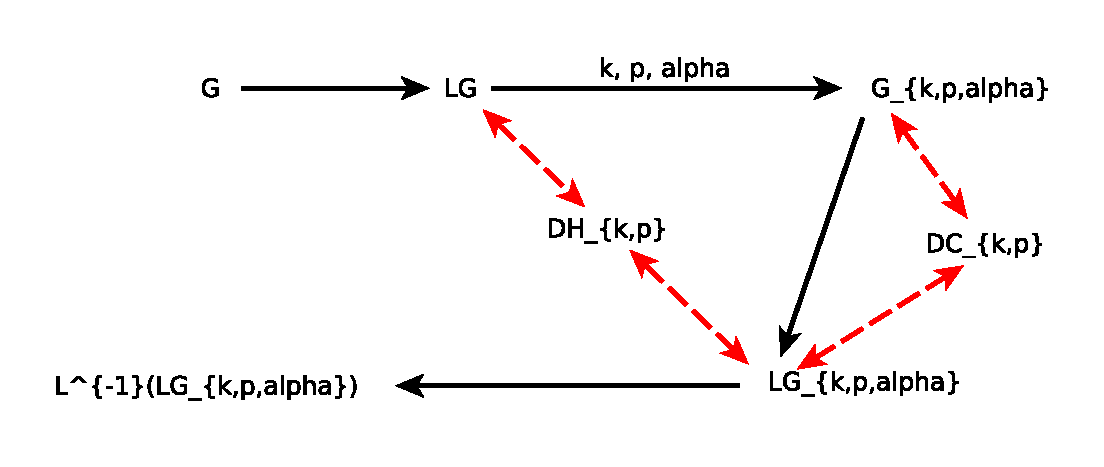
\includegraphics[scale=0.750]{recapProtocoleEtude.eps}
\caption{\'Etapes de l'exp\'erimentation :  \\
1) On g\'en\`ere le graphe $G$ et son line-graphe $LG$;\\ 
2) On modifie $k$ cases la $\alpha^{ieme}$ fois selon la repartition $p$ pour obtenir le graphe $G_{k,p,\alpha}$;\\ 
3) On applique les algorithmes de couverture et de correction pour avoir un line-graphe $LG_{k,p,\alpha}$. $LG_{k,p,\alpha}$ et  $G_{k,p,\alpha}$ diff\`erent de $DC_{k,p,\alpha}$ ar\^etes. $LG_{k,p,\alpha}$ a $DH_{k,p,\alpha}$ cases modifi\'ees par rapport \`a $LG$; 
\\ 4) $L^{-1}(LG_{k,p,\alpha})$ est le graphe racine de $LG_{k,p,\alpha}$. }
\label{recapProtocoleEtude} 
\end{figure}
% ------------  figure recap Protocole Etude  ----------------------
%\FloatBarrier
\newline


% correction du graphe
% 1) comment je selectionne (choisis) les sommets -1
%		- remise: on selectionne un sommet de sommets -1 selon une methode puis on la corrige. Ensuite, on applique notre couple d'algorithme  sur le graphe corrig\'e. On reprend l'operation tant que graphe corrige n'est pas un line-graphe    
%		- sans remise: On choisit une permutation des sommets de sommets-1 puis on les corrige les uns a la suite des autres.Les sommets dans la permutation sont ordonnee selon  la methode suivante:
% 		* degre min : les sommets sont ranges par ordre croissant de leur degre.
%		* cout min : les sommets sont ranges par ordre croissant de leur cout. Le cout est la somme du poids de chaque case modifi\'e.
%		* aleatoire :  les sommets sont ranges sans condition prealable.
%			* aleatoire * cout min * degre min
%correction
Soit ${\cal C}$ l'ensemble des sommets n'\'etant couverts par aucune clique apr\`es l'algorithme de couverture.
La correction de la matrice $M_{k,p,\alpha}$ est n\'ecessaire s'il existe des sommets appartenant \`a ${\cal C}$. 
\newline
Nous distinguons deux modes d'ex\'ecution de notre algorithme de correction:
\begin{enumerate}
	\item Mode avec remise :
				\newline
				\noindent 1. Ex\'ecution algorithme de couverture, {\bf return} ${\cal C}$ \\
				~2. \indent {\bf Tant que} ${\cal C}$ n'est pas vide\\ 
				~3.	       	\indent~~~~~~~~Correction d'un sommet de ${\cal C}$  \\
				~4.	       	\indent~~~~~~~~Ex\'ecution algorithme de couverture, {\bf return} ${\cal C}$ \\
	\item Mode sans remise :
				\newline
				\noindent 1. Ex\'ecution algorithme de couverture, {\bf return} ${\cal C}$ \\
				~2. \indent {\bf Tant que} ${\cal C}$ n'est pas vide\\ 
				~3.	       	\indent~~~~~~~~Correction d'un sommet de ${\cal C}$  \\
				~4.	       	\indent~~~~~~~~Mise \`a jour du sommet  de ${\cal C}$  \\
\end{enumerate}
\`A chaque \'etape $3$ dans les deux modes, un sommet de $\cal C$ est choisi selon :
\begin{enumerate} [label = (\alph*)]
\item {\em Degr\'e minimum} : le sommet de degr\'e minimum est s\'electionn\'e. 
\item {\em Co\^ut minimum} : le sommet de  co\^ut de compression minimum est s\'electionn\'e. Le co\^ut de compression est la somme des co\^uts de chaque case modifi\'ee. 
\item {\em Al\'eatoire} : le sommet est s\'electionn\'e al\'eatoirement parmi les sommets de $\cal C$.
\end{enumerate}
La correction de chaque sommet de ${\cal C}$ implique l'ajout et la suppression des ar\^etes du graphe. Nous souhaitons orienter les d\'ecisions de l'algorithme de correction de telle sorte qu'il ajoute  ou supprime uniquement des ar\^etes ou 
qu'il r\'ealise les deux op\'erations.
 Nous  priorisons une op\'eration en attribuant des co\^uts diff\'erents \`a  la modification d'ar\^etes.
Nous distinguons trois types d'op\'erations que nous appelons {\em fonctions de co\^ut} :
\begin{enumerate}[label=(\roman*)]
\item {\em Unitaire} : l'ajout et la suppression d'une ar\^ete ont un m\^eme co\^ut c'est-\`a-dire $1$.
\item {\em Ajout} : l'ajout d'une ar\^ete a un co\^ut de $1$ et la suppression a un co\^ut de $2$.
\item {\em Suppression} : l'ajout d'une ar\^ete a un co\^ut de $2$ et la suppression a un co\^ut de $1$.
\end{enumerate}
Nous rappelons que la distance de correction n'est pas la somme de toutes les  modifications d'ar\^etes r\'ealis\'ees. En effet, une ar\^ete  supprim\'ee et ajout\'ee plusieurs fois (pour diff\'erents sommets de ${\cal C}$) n'est comptabilis\'ee qu'une fois et son co\^ut est appliqu\'e selon la fonction de co\^ut.
\newline


\'Etant donn\'ee que nous avons $3$ fonctions de co\^ut, $2$ modes de correction et $3$  s\'elections possibles des sommets, nous nous retrouvons avec $18$ approches de correction de sommets et il est fastidieux de les interpr\'eter sur une m\^eme figure.
Ainsi nous nous limitons \`a la fonction de co\^ut {\em unitaire} dans un premier temps et nous consid\'erons les approches de correction suivantes : $1a$, $1b$, $2a$, $2b$, $2c$.  
La lecture de l'approche de correction $(1a)$ est le suivant : $1)$ avec remise et $a)$ le degr\'e minimum.
L'approche $(1c)$ n'est d'aucune utilit\'e car l'algorithme de correction ne parvient pas \`a fournir un line-graphe. En effet, l'ensemble $\cal C$ croit lin\'eairement \`a chaque \'etape de correction et la correction devient une boucle infinie.
Le tableau \ref{tab:recapApprocheCorrection} r\'esume les approches de correction retenues dans l'analyse des performances de l'algorithme de correction.
% ------------ tableau recapitulatif -----------------------
\begin{table}[h]
   \centering
   \caption{\label{tab:recapApprocheCorrection} Tableau r\'ecapitulatif des approches de corrections }
   \begin{tabular}{|l|c|c|r|}
   	\hline
  	Mode & choix sommets & fonction de co\^ut  \\
  	\hline
%  	Sans Remise & Degre Min & unitaire & 1  \\
%  	\cline{1-9}     & \cline{1-3} & ajout       & 1  \\
	 & 
								\multirow{3}{*}{degr\'e minimum} & unitaire \\
															  & & ajout \\
									
												& & suppression \\
											
								\cline{2-3}
	Sans remise						& 
								\multirow{3}{*}{co\^ut minimum} & unitaire \\
															  & & ajout \\
															  & & suppression \\
															  \cline{2-3}								  
							& 
								\multirow{3}{*}{al\'eatoire} & unitaire \\
															  & & ajout \\
															  & & suppression \\
															  \hline
															  \hline									 
	 & 
								\multirow{3}{*}{degr\'e minimum} & unitaire \\
															  & & ajout \\
															  & & suppression \\
															 \cline{2-3}
	Avec remise						& 
								\multirow{3}{*}{co\^ut minimum} & unitaire \\
															  & & ajout \\
															  & & suppression \\
															  \hline															  
   \end{tabular}
\end{table}
% ------------ tableau recapitulatif -----------------------
\newline

Nous recherchons l'approche qui traite le probl\`eme {\em Proxi-Line} c'est-\`a-dire le mode qui majore la distance line de $G_{k,p}$ par la distance de correction entre $LG_{k,p}$ et $G_{k,p}$.
Une fois le meilleur mode trouv\'e, nous comparons les fonctions de co\^ut $i$, $2i$ et $3i$ avec ce mode pour trouver l'influence de la fonction de co\^ut sur les distances de correction.

%---- decription protocole d'etude --> fin
	\subsection{Analyses des r\'esultats }

	Nous d\'ebutons l'interpr\'etation de nos r\'esultats par l'analyse des distributions des distances de Hamming avec l'approche de correction {\em al\'eatoire sans remise} $(2c)$ et  la fonction de co\^ut {\em unitaire} $(3i)$.
	Ensuite, nous expliquons le choix de l'approche $(2c)$  pour la correction des sommets. 
	Nous pr\'esentons \'egalement le meilleur compromis dans la repartition des $k$ cases modifi\'ees et la relation existante entre les distances de correction et de Hamming.
	Enfin,  nous montrons que l'approche $(2c)$ fournit des distributions de distances de correction et de Hamming identiques, quelles que soient la fonction de co\^ut $(i), (2i), (3i)$ et la repartition $k$ choisies.
		\subsubsection{Interpr\'etation du mode de correction {\em al\'eatoire sans remise}}
			\label{experimentation1InterpretationModeAleatoireSansRemise}
			

% debut explication aprroche aleatoire sans remise avec cout unitaire 
Nous supposons que $p=0.5$ c'est-\`a-dire qu'il y'a autant de cases {\em fausses n\'egatives} que de cases {\em fausses positives} dans la matrice $M_{k,p}$.
\newline
Nous repr\'esentons les distributions des distances de correction et de Hamming, la fonction de repartition de la corr\'elation entre ces distances  et la fonction cumulative de la distance de Hamming. 
La distribution des distances de correction indique la proportion de graphes $LG_{k,p,\alpha}$ qui ont le m\^eme ensemble d'ar\^etes que les graphes $G_{k,p,\alpha}$. En ce qui concerne la distribution des distances de Hamming, elle indique  la proportion de graphes $LG_{k,p,\alpha}$ qui ont le m\^eme ensemble d'ar\^etes que les graphes $LG$.
La corr\'elation entre les distances de correction et de Hamming, not\'ee {\em correlation\_DC\_DH}, est calcul\'ee avec la formule \ref{correlation_correction_hamming}. Sa fonction de repartition $F_k(x)$ indique le nombre de corr\'elations inf\'erieures \`a une valeur de corr\'elation $x$ donn\'ee.
Quant \`a la fonction cumulative de la distance de Hamming, elle montre l'\'evolution du nombre de cases modifi\'ees de la matrice $M'_{k,p}$ en fonction du nombre de line-graphes  construits $LG$.
\newline
%\vspace{-0.5cm}
% -------------------- figure simulation_distanceMoyenDLDH_k_0_aleatoire_p_05 ------------------------
\begin{figure}[htb!] 
\centering
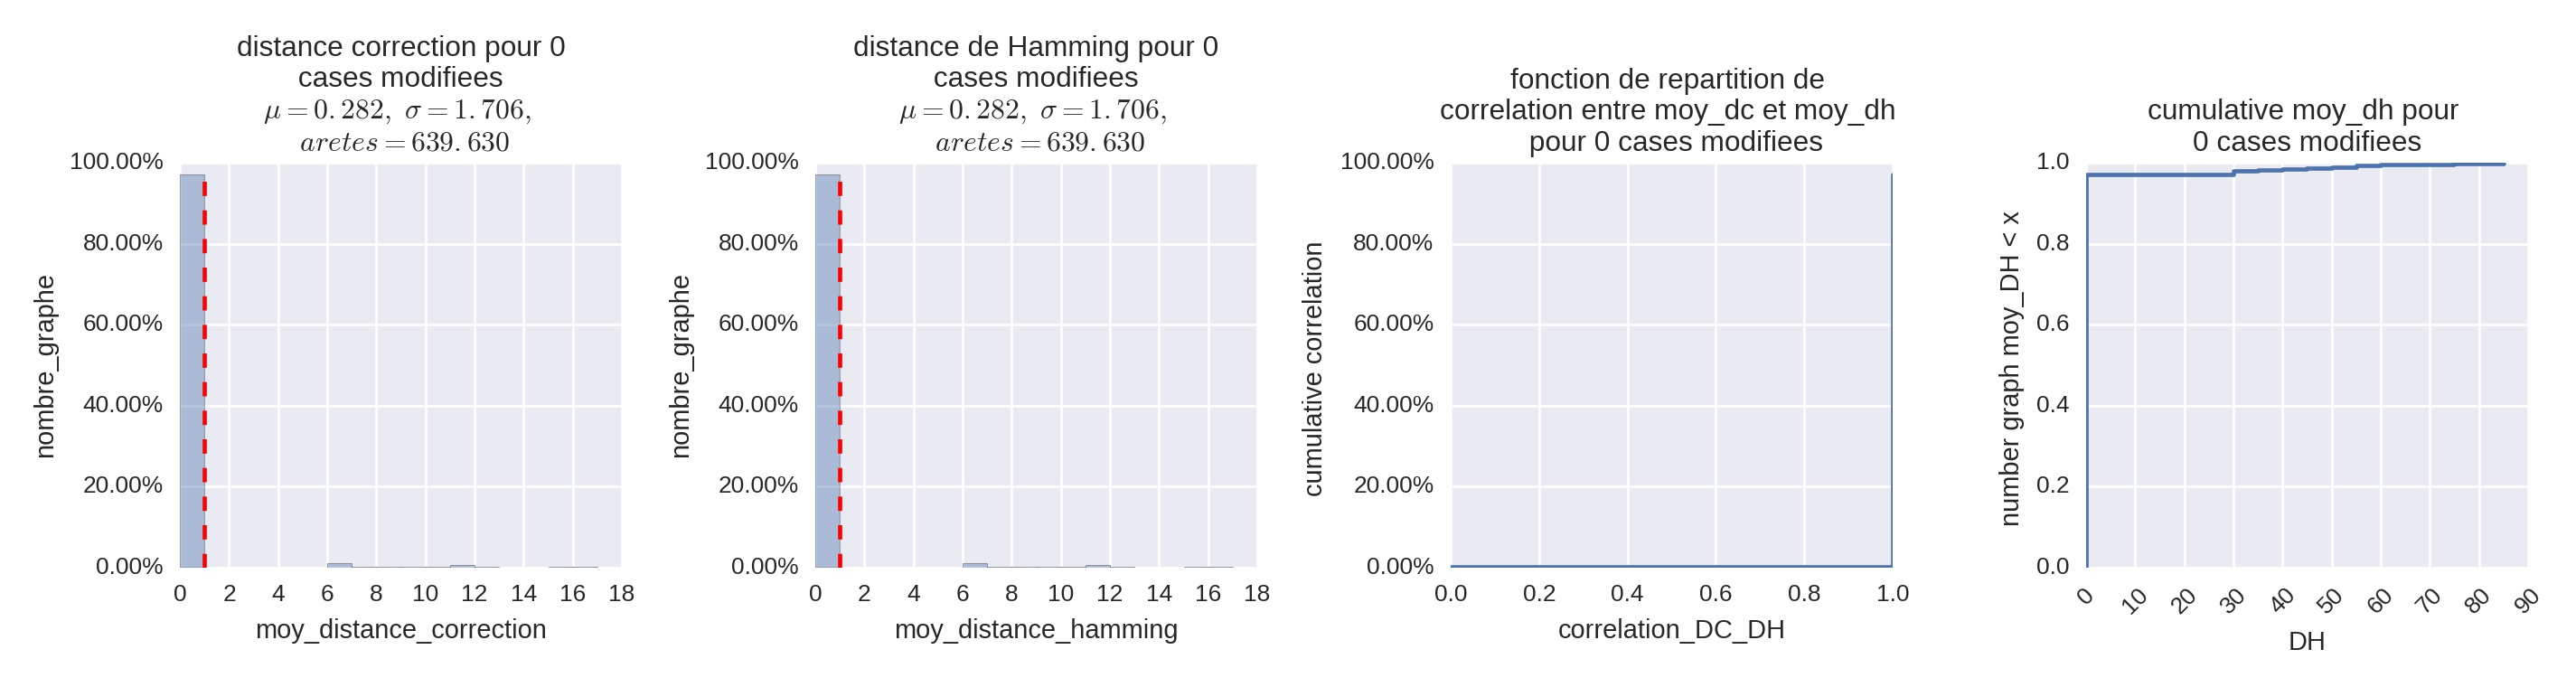
\includegraphics[width=500pt,height=160pt]{simulation_distanceMoyenDLDH_k_0_aleatoire_p_05.jpeg}
\caption{ Approche de correction al\'eatoire sans remise \`a co\^ut unitaire pour $k =0 $ case modifi\'ee. La premi\`ere colonne repr\'esente la distribution des distances de correction $moy\_DC_{0,0.5}$. La seconde colonne est la distribution des distances de Hamming $moy\_DH_{0,0.5}$. La troisi\`eme colonne  est la fonction de repartition de la corr\'elation entre les distances de correction et de Hamming avec en abscisse la corr\'elation entre ces distances (correlation\_DC\_DH).  La quatri\`eme colonne est la fonction cumulative des distances de Hamming.}
\label{sansremise_unitaire_distanceMoyenDCDH_k_0_aleatoire_p_05} 
\end{figure}
\FloatBarrier
% -------------------- figure simulation_distanceMoyenDLDH_k_0_aleatoire_p_05 -----------------------

Les figures \ref{sansremise_unitaire_distanceMoyenDCDH_k_0_aleatoire_p_05} et \ref{sansremise_unitaire_distanceMoyenDCDH_k_1_2_5_9_aleatoire_p_05} pr\'esentent les courbes respectives pour $k=0$ et $k \in \{1,2,5,9\}$ cases modifi\'ees. 
La colonne $1$ indique la distribution des distances de correction, la colonne $2$ est la colonne de la distribution des distances de Hamming, la colonne $3$ est associ\'ee \`a la fonction de repartition de la corr\'elation entre les distances de correction et de Hamming avec en abscisse la corr\'elation entre ces distances ({\em correlation\_DC\_DH)}. 
Et la colonne $4$ est celle de la fonction cumulative des distances de Hamming.
Dans les colonnes $1$ et $2$, les distributions se divisent en deux zones: 
\begin{itemize}
\item Zone {\em gauche} ou {\em am\'eliorante} : elle correspond aux batonnets de l'intervalle $[0,k]$. Cet intervalle  am\'eliore l'ensemble $E'_{k,p,\alpha}$ des ar\^etes du graphe $LG_{k,p,\alpha}$ pour que $E'_{k,p,\alpha}$ soit identique \`a l'ensemble $E_{LG}$ des ar\^etes du graphe $LG$. Si $moy\_DH_{k,p} \rightarrow 0$ alors $LG_{k,p,\alpha}$ est tr\`es proche de $LG$. Si $moy\_DH_{k,p} \rightarrow k$ alors les matrices des graphes $LG_{k,p,\alpha}$ et $LG$ diff\`erent de $k$ cases et ces cases sont les $k$ cases modifi\'ees dans $LG$.
\item Zone {\em droite} ou {\em d\'egradante} : elle correspond aux batonnets de l'intervalle $]k, +\infty[$. Cet intervalle d\'et\'eriore  l'ensemble $E'_{k,p,\alpha}$ des ar\^etes du graphe $LG_{k,p,\alpha}$. Ainsi, le line-graphe $LG_{k,p,\alpha}$ s'\'eloigne de $LG$ quand $moy\_DH_{k,p} \rightarrow +\infty$.
\end{itemize}
Ces deux zones sont s\'epar\'ees par une droite en pointill\'ee d'\'equation $y = k$.  Cette droite d\'esigne le nombre de cases modifi\'ees dans le line-graphe $LG$.
\newline

Pour $k=0$ case modifi\'ee, nous v\'erifions que nos algorithmes sont coh\'erents c'est-\`a-dire que la phase de correction est inutile. En effet, nous avons $100\%$ de graphes $G_{k,p,\alpha}, LG_{k,p,\alpha}, LG$ qui ont les m\^emes ensembles d'ar\^etes et cela implique que $moy\_DH_{0,0.5} = moy\_DC_{0,0.5} = 0$. D'o\`u le seul batonnet dans les colonnes $1$ et $2$. Par ailleurs, la fonction de repartition de la corr\'elation et la fonction cumulative des distances de Hamming sont d\'efinies par les \'equations \ref{eqCorrelMoyDCDH} (a) et (b)  respectivement.
\begin{equation}
\label{eqCorrelMoyDCDH}
F_k(x_1) = \left\{
	\begin{aligned}
	0 \hspace{1 em} si \hspace{1 em} x_1 < 1 \\
	100  \hspace{1 em}  si  \hspace{1 em}  x_1 = 1
	\end{aligned}
	\right.(a)
	\\~~~~~~~
	y_{cumulDH}^{0}(x) = 1  \hspace{1 em}  si  \hspace{1 em}   x \in \N (b)
\end{equation}
%\begin{equation}
%\label{eqCumulMoyDH}
%y_{cumulDH}^{0}(x) = 1  \hspace{1 em}  si  \hspace{1 em}   x \in \N
%\end{equation}
avec $x_1$ la corr\'elation entre les distances et $x$ le nombre d'ar\^etes modifi\'ees.
Les valeurs des distances de Hamming sont \'egales \`a $0$ donc sa fonction cumulative $y_{cumulDH}^{k}$ vaut $1$. 
L'\'equation  \ref{eqCorrelMoyDCDH}(a) s'interpr\`ete comme suit : $F_k(x) = 100\%$ des line-graphes ont leurs distances de correction et de Hamming corr\'el\'ees ($x = 1$).
\newline

% k = {1,2}
Pour $k \in \{1,2\}$, le pic des histogrammes se localise dans la zone {\em am\'eliorante} des colonnes $1$ et $2$ de la figure \ref{sansremise_unitaire_distanceMoyenDCDH_k_1_2_5_9_aleatoire_p_05} et son pourcentage est sup\'erieur \`a $50\%$. 
Les autres batonnets sont dans la zone {\em d\'egradante} et leur pic a un pourcentage inf\'erieur \`a $10\%$ en moyenne. 
Dans la colonne $1$ de la figure \ref{sansremise_unitaire_distanceMoyenDCDH_k_1_2_5_9_aleatoire_p_05}, le pic correspond aux $k$ cases modifi\'ees du graphe $G_{k,p,\alpha}$ et son pourcentage est identique \`a celui du pic de la colonne $2$. 
Le pic de la colonne $2$, correspondant \`a $moy\_DH_{k,0.5} = 0$, signifie que  $LG$ et $LG_{k,p,\alpha}$ ont le m\^eme ensemble d'ar\^etes. Ainsi, les $k \le 2$ cases modifi\'ees sont supprim\'ees de la matrice $M'_{k,p,\alpha}$ lorsque $moy\_DC_{k,0.5} \le k$.
Cependant, les distances de correction et de Hamming ont approximativement les m\^emes valeurs lorsque $moy\_DC_{k,0.5} > k$ ($moy\_DC_{k,0.5}$ est dans la partie {\em d\'egradante} de la figure \ref{sansremise_unitaire_distanceMoyenDCDH_k_1_2_5_9_aleatoire_p_05}). 
Cela s'explique par le fait que les distances $moy\_DC_{k,0.5}$ et $moy\_DH_{k,0.5}$ sont corr\'el\'ees. Nous d\'etaillons la notion de corr\'elation de distances dans la section \ref{relationMoyDHmoyDC}.
% ---- a ajouter dans la partie correlation
%En effet, la colonne $3$ de la figure \ref{sansremise_unitaire_distanceMoyenDLDH_k_1_2_5_9_aleatoire_p_05} d\'esigne les corr\'elations entre ces distances. Pour une corr\'elation $x > 0.3$, $F_k(x) > 60\%$ et  pour $x \le 0.3$, $F_k(x) < 5\%$. Or $F_k(x)\rightarrow 0\%$ signifie que $moy\_DL$ est \'egale \`a $k$ ($moy\_DL = k$) et $moy\_DH$ tend vers $k$ ($moy\_DH \rightarrow k$). Donc $F_k(x) < 5\%$ implique que $moy\_DL = k$ et $moy\_DH \approx k$.
Ainsi, les distances de correction et de Hamming sont corr\'el\'ees dans $\eta_k = 5\%$ des line-graphes $LG_{k,p,\alpha}$ et le line-graphe $LG_{k,p,\alpha}$ devient le line-graphe initial $LG$ si nous corrigons les $DC$ cases modifi\'ees du graphe $LG_{k,p,\alpha}$. 
La variable $\eta_k$ est la proportion de line-graphes dont les distances de correction et de Hamming sont fortement corr\'el\'ees.
\newline

% ------------------- figure permut_distanceMoyenDLDH_k_1_2_5_9_aleatoire_p_05 ------------------
\begin{figure}[htb!] 
%\centering
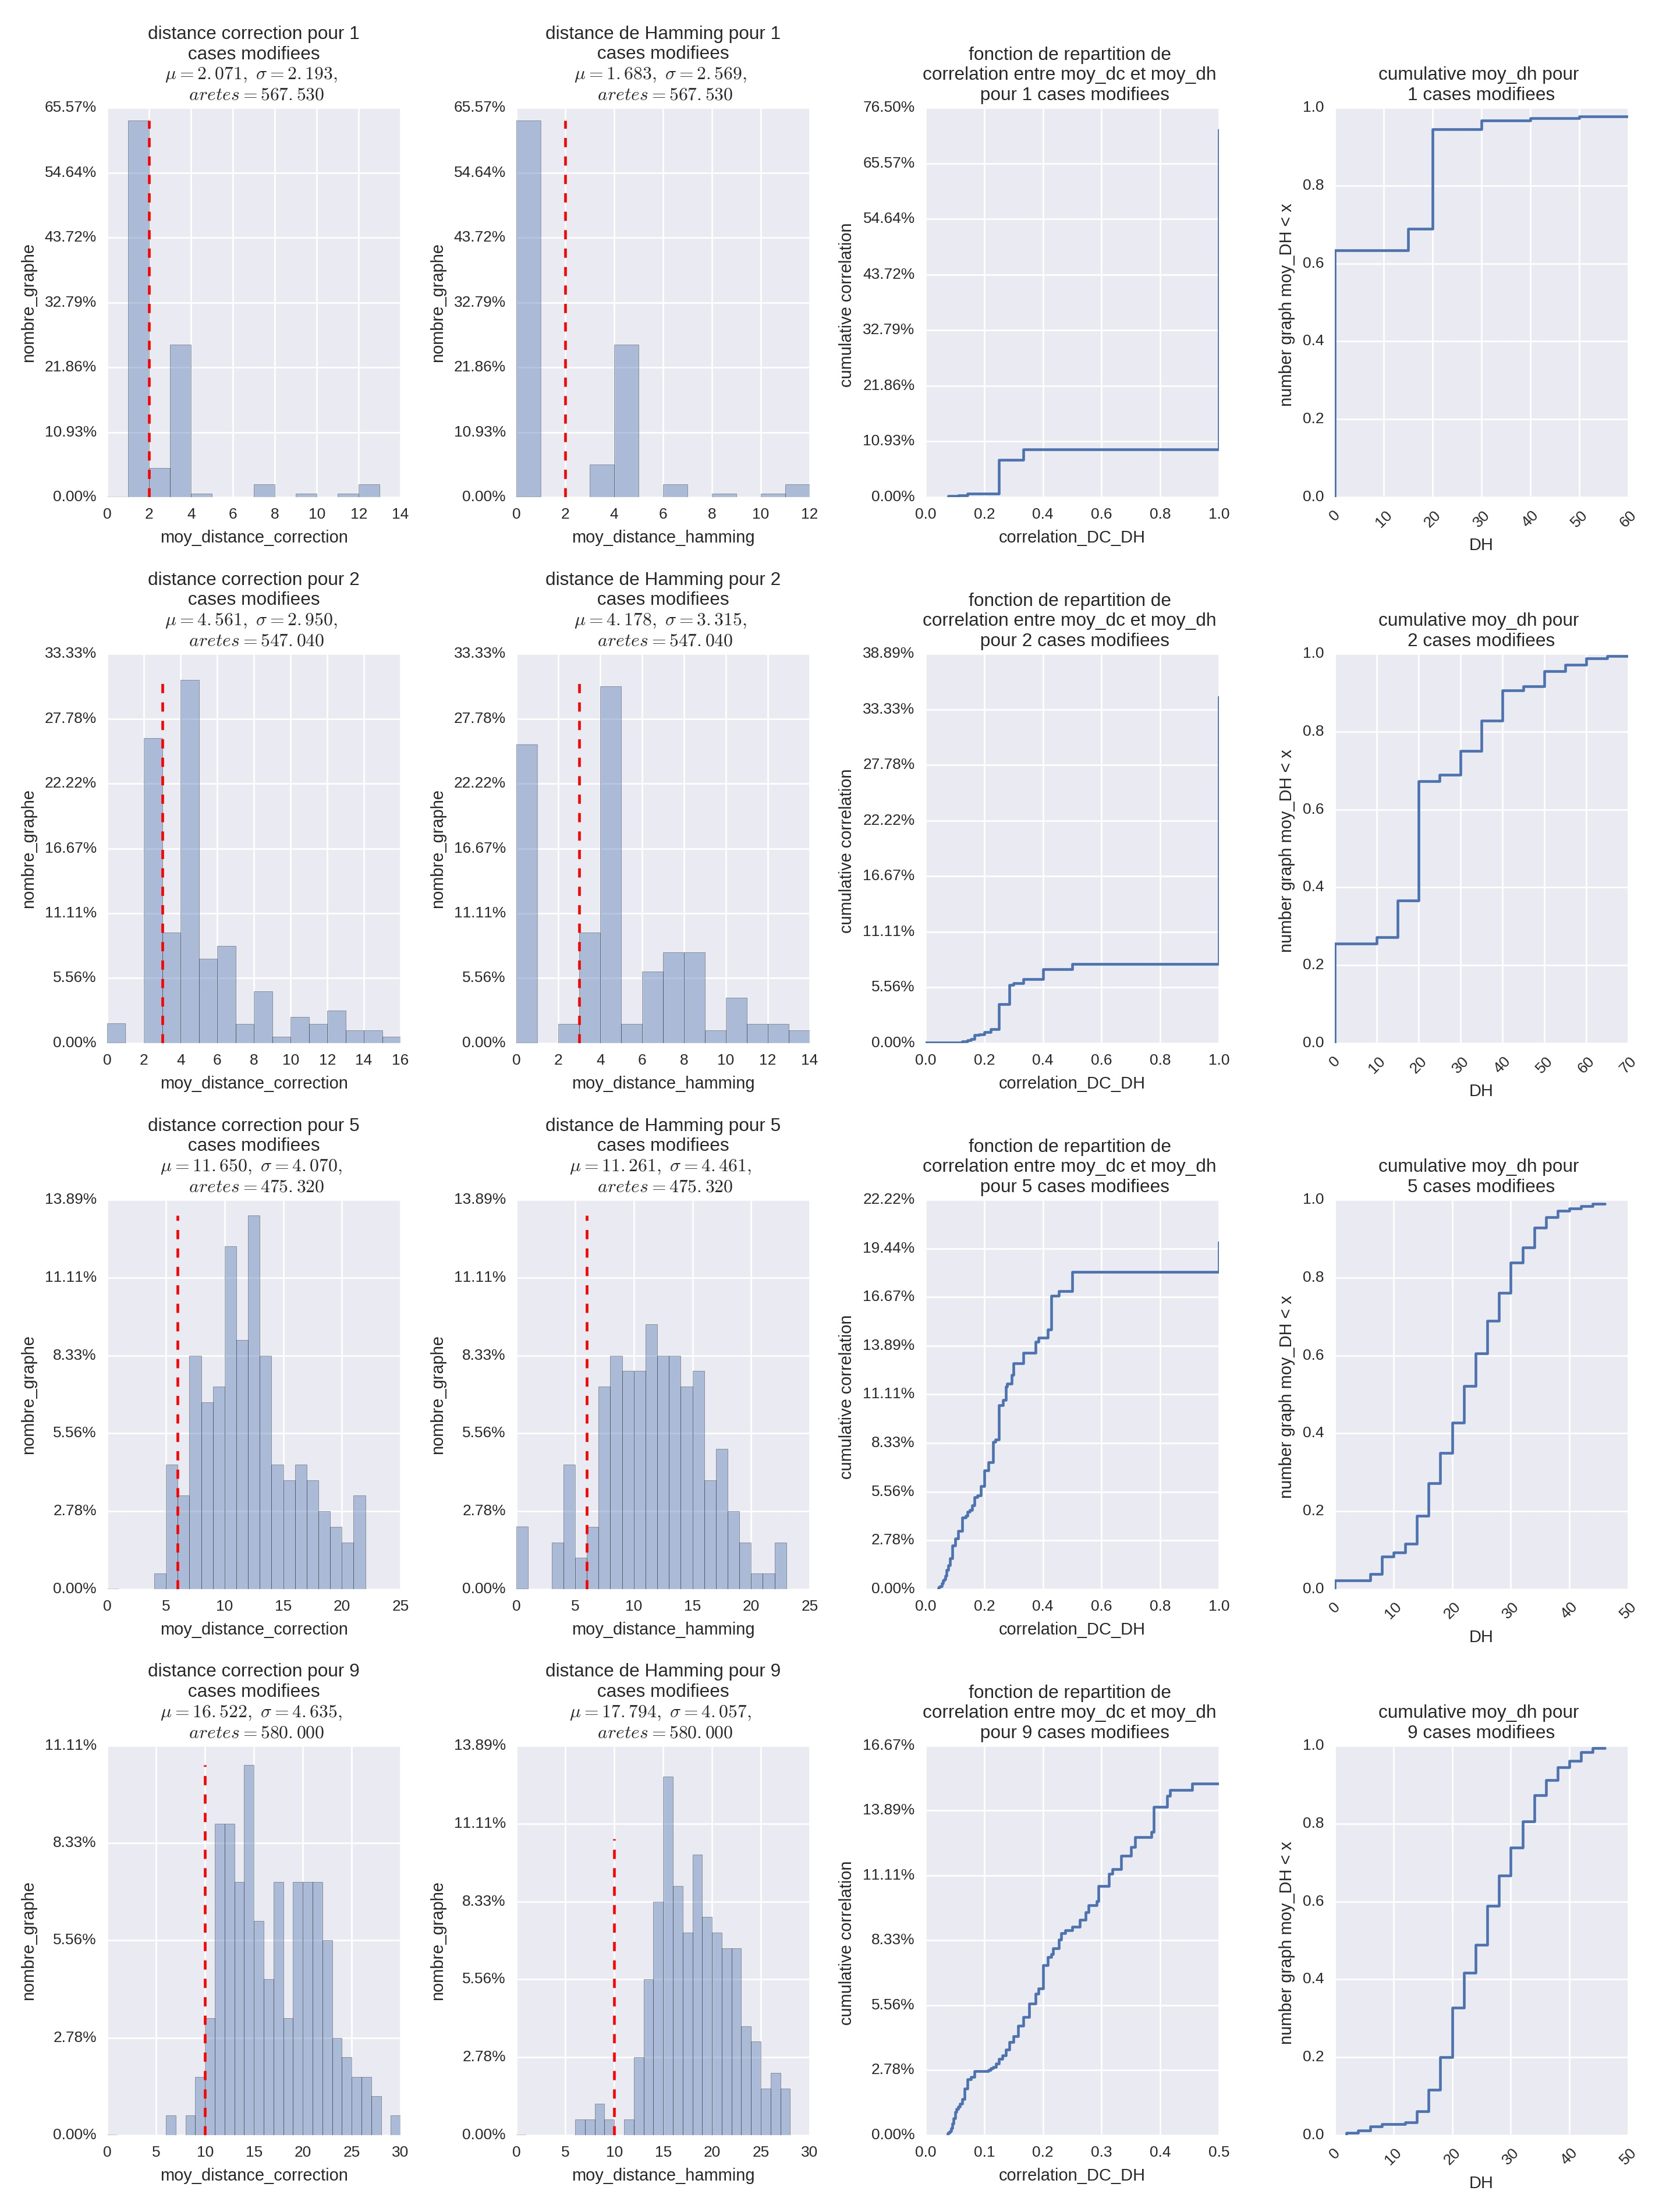
\includegraphics[width=550pt,height=570pt]{permut_distanceMoyenDLDH_k_1_2_5_9_aleatoire_p_05.jpeg}
\caption{ Approche de correction al\'eatoire sans remise \`a co\^ut unitaire pour $k =\{1,2,5,9\} $ cases modifi\'ees :
 La premi\`ere colonne repr\'esente la distribution des distances de correction $moy\_DC_{k,0.5}$. La seconde colonne est la distribution des distances de Hamming $moy\_DH_{k,0.5}$. 
 La troisi\`eme colonne  est la fonction de repartition de la corr\'elation entre les distances de correction et de Hamming avec en abscisse la corr\'elation entre ces distances (correlation\_DC\_DH).  
 La quatri\`eme colonne est la fonction cumulative des distances de Hamming. 
 La premi\`ere ligne est associ\'ee \`a $k=1$ case modifi\'ee, 
 la seconde ligne \`a $k=2$ cases modifi\'ees, 
 la troisi\`eme ligne \`a $5$ cases modifi\'ees et enfin 
 la derni\`ere \`a $9$ cases modifi\'ees.
 }
\label{sansremise_unitaire_distanceMoyenDCDH_k_1_2_5_9_aleatoire_p_05} 
\end{figure}
\FloatBarrier
% ----------------- figure permut_distanceMoyenDLDH_k_1_2_5_9_aleatoire_p_05 ---------------------

% k = 5
Pour $k = 5$, le pic se trouve toujours dans la zone {\em am\'eliorante} des colonnes $1$ et $2$ de la figure \ref{sansremise_unitaire_distanceMoyenDCDH_k_1_2_5_9_aleatoire_p_05} mais son pourcentage baisse significativement \`a $15.69\%$ (voir la ligne $3$). 
Le nombre de  line-graphes dans la zone {\em d\'egradante} dans les colonnes $1$ et $2$ augmente tout comme les distances de correction et de Hamming qui atteignent  jusqu'\`a $45$ ar\^etes.
La variable $\eta_k$ est \'egale \`a  $18.38\%$ de line-graphes $LG_{k,p,\alpha}$ (voir ligne $3$ de la colonne $3$ de la figure \ref{sansremise_unitaire_distanceMoyenDCDH_k_1_2_5_9_aleatoire_p_05}).
Cette augmentation provient de la baisse du pourcentage du pic de la zone {\em am\'eliorante} au profit de la zone {\em d\'egradante} et la plupart des graphes appartenant \`a cette zone ont leurs distances de correction et de Hamming corr\'el\'ees.
Les $15.69\%$  de line-graphes $LG_{k,p,\alpha}$ identiques \`a $LG$ s'expliquent par le type de cases modifi\'ees et l'emplacement des ar\^etes dans le graphe $LG$.  En effet, ces cases modifi\'ees sont des {\em fausses n\'egatives} et ces ar\^etes supprim\'ees n'appartiennent pas \`a des cliques voisines. Toutefois, quelque soit le type de cases modifi\'ees, notre couple d'algorithmes ajoutent beaucoup d'ar\^etes pour obtenir le line-graphe $LG_{k,p,\alpha}$ lorsque les cases sont reparties avec $p = 0.5$. Par exemple, nous avons constat\'e, en moyenne, $10$ \`a $20$ ar\^etes diff\'erentes pour $k=5$ cases modifi\'ees dans nos exp\'erimentations. 
Par ailleurs, nous remarquons qu'il existe des graphes dans lesquels la distance de correction est inf\'erieure \`a $k$. Tel est le cas pour $k = 5$ ou nous avons $moy\_DC_{k,0.5} = 3$ et $nombre\_graphe = 0.14\%$ dans la colonne $1$  de la figure \ref{sansremise_unitaire_distanceMoyenDCDH_k_1_2_5_9_aleatoire_p_05}.
En effet, les cases modifi\'ees sont des cases {\em fausses n\'egatives}. Ces ar\^etes supprim\'ees de $LG$ appartiennent \`a la m\^eme clique et certaines ar\^etes sont ajout\'ees de telle sorte que la clique se partitionne en deux cliques.   
%les aretes appartiennent a une meme cliques  de tel sorte qu'il ajoute certains aretes qui sindent la clique en deux cliques
%1) lalgo ajoute des aretes
%2) ces aretes  appartiennent a la meme clique et elles sont ajoutes de tel sorte que il forme deux cliques
\newline 

% k = 9
Enfin, pour $k=9$, la distribution des valeurs de distances est dans la zone {\em d\'egradante} et le pic est \`a $moy\_DC_{k,0.5} = 23$ cases modifi\'ees avec un pourcentage de $6\%$ line-graphes.  
En comparant les pourcentages des distances $moy\_DC_{k,0.5}$ et $moy\_DH_{k,0.5}$, nous constatons qu'ils ne sont pas identiques comme pour $k \le 5$. En effet, certaines cases modifi\'ees ne sont pas corrig\'ees car l'algorithme de correction modifie \'enorm\'ement de cases qui sont diff\'erentes des $k$ cases et ce taux croit quand  $moy\_DC_{k,0.5}$ est \'elev\'e. 
Le taux de cases corrig\'ees est de $53.38\%$ en moyenne.
La variable $\eta_k$ passe \`a $22\%$ de line-graphes $LG_{k,p,\alpha}$ parce que la correction a modifi\'ee des cases diff\'erentes des $k$ cases. Cependant les distances de correction et de Hamming restent toujours corr\'el\'ees et $3\%$ line-graphes $LG_{k,p,\alpha}$ ont le m\^eme ensemble d'ar\^etes que $LG$ (voir ligne $4$ de la colonne $3$ de la figure \ref{sansremise_unitaire_distanceMoyenDCDH_k_1_2_5_9_aleatoire_p_05}).
C'est pourquoi, les courbes de  $F_k(x)$ et $y_{cumulDH}^{k}$ ont cette forme enrob\'ee proche de la fonction  sigmoide de param\`etre $\lambda \le -15$. Pour rappel, nous pr\'ecisons que ces courbes  tendent vers la fonction suivante $f_{\lambda}(x) = \frac{1}{1+e^{\lambda * (x-0.5)}}$.
\newline
Les  cases modifi\'ees $k \in \{1,\cdots,9\}$ sont pr\'esent\'ees dans les figures 
 \ref{sansremise_unitaire_distanceMoyenDCDH_k_1_5_aleatoire_p_05} et  
\ref{sansremise_unitaire_distanceMoyenDCDH_k_6_9_aleatoire_p_05} de l'annexe \ref{annexe_distribution_0_9}.
\newline
% fin explication mode aleatoire sans remise avec cout unitaire 

L'approche de correction $(2c)$ nous montre que les distances de correction et de Hamming se d\'egradent quand le nombre $k$ de cases modifi\'ees augmentent. En fait, pour $k \le 5$, le nombre de line-graphes $LG_{k,p,\alpha}$ identiques \`a $LG$ est sup\'erieur \`a $nombre\_graphe = 25\%$ avec des distances de correction $moy\_DC_{k,0.5} = k$. Pour des distances $moy\_DC_{k,0.5} = 2 \times k$, les  $k$ cases modifi\'ees sont corrig\'ees. 
Des cases erron\'ees sont ajout\'ees pendant l'ex\'ecution de l'algorithme de correction mais elles sont peu nombreuses. Nous pouvons consid\'erer ces cases comme la pr\'ecision de notre algorithme  car ces cases indiquent le nombre de cases \`a modifier pour obtenir $LG$. Ainsi la distance de correction est major\'ee par le nombre de cases $k$ modifi\'ees.
Cependant, au d\'el\`a de $k > 5$,  la distance de correction $moy\_DC_{k,0.5}$ double et moins de $50\%$ des $k$ cases sont corrig\'ees. Les cases erron\'ees proviennent de l'ajout et la suppression d'ar\^etes dans le line-graphe $LG'_{k,p,\alpha}$ \'etant donn\'ee que la fonction de co\^ut est {\em unitaire}. La distance de correction est major\'ee par $2 \times k$ en moyenne.
\newline

{\bf Conclusion} : l'approche de correction {\em al\'eatoire sans remise} $(2c)$ propose des line-graphes $LG_{k,p}$  identiques \`a $LG$ quand $k \le 5$. Dans ce cas, le probl\`eme {\em Proxi-Line} est trait\'e car la distance line est major\'ee par $k$. 
Toutefois, le nombre de cases \`a corriger apr\`es l'ex\'ecution de notre couple d'algorithmes est faible lorsque la distance de correction est inf\'erieure au double de $k$ ($moy\_DC_{k,0.5} = 2 \times k$) avec $k>5$. Cela conduit \`a majorer la distance line par le double des cases erron\'ees.
En outre, pour $k>5$, le pourcentage  $\eta_k$ de corr\'elation entre $moy\_DC_{k,0.5}$ et $moy\_DH_{k,0.5}$ croit. Nous allons \'etudier l'\'evolution de $\eta_k$  dans le paragraphe \ref{relationMoyDHmoyDC} mais nous commencons par la comparaison des diff\'erentes approches de correction pour en d\'eduire celle qui minimise les distances de correction ou de Hamming.


		\subsubsection{Comparaison des modes de correction}
			
Nous recherchons la meilleure approche de correction parmi les cinq  \'enum\'er\'ees dans le tableau \ref{tab:recapApprocheCorrection}.
Pour ce faire, nous disposons des distributions des distances de correction et de Hamming, des fonctions de repartition de ces distributions et aussi des moyennes de distances de correction et de Hamming associ\'ees aux $k$ cases modifi\'ees. Les distributions des distances de correction et de Hamming sont obtenues avec  $p=0.5$ et la fonction de co\^ut est {\em unitaire}.
Les distributions de distances de chaque approche sont regroup\'ees dans les colonnes $1$ et $2$ dans les figures en annexes \ref{annexe_distribution_0_9}.
%Nous avons montr\'e dans le paragraphe \ref{relationMoyDHmoyDL} que la distance line peut \^etre utilis\'ee comme m\'etrique de comparaison entre deux graphes. Cependant, 
Nous d\'ecidons d'utiliser la moyenne des distances de Hamming pour la comparaison de approches de correction parce qu'il est facile de d\'eterminer le nombre de cases modifi\'ees \'etant donn\'ee que nous connaissons les line-graphes $LG$ et $LG_{k,p}$. 
\newline

%ARRETER ICI
%
%Soit $G_{k,p,\alpha}^{i}$  le $i^{ieme}$  graphe g\'en\'er\'e contenant $k$ cases modifi\'ees la $\alpha^{ieme}$ fois avec la repartition $p=0.5$ des $k$ cases. Nous le notons $G_{k,\alpha}^{i}$ avec $ 0 \le i \le 500$ et $\alpha \le \alpha_{max}$. \\
%Soit $DC_k^i$ le nombre de cases corrig\'ees par l'algorithme de correction pour le graphe $G_{k,\alpha}^{i}$.\\
%$\bar{DC_k^i}$ est la moyenne de $DC_k^i$ pour les $\alpha_{max}$ graphes $G_{k,\alpha}^{i}$.\\ 
%$\bar{DC_k}$ est la moyenne de $\bar{DC_k^i}$ pour $500$ graphes contenant $k$ cases modifi\'ees.\\
%Nous choisissons $\bar{DC_k}$ comme crit\`ere de comparaison des approches de corrections. %parce que A TROUVER 
%\newline
Soit $G_{k,p,\alpha}^{i}$  le $i^{ieme}$  graphe g\'en\'er\'e contenant $k$ cases modifi\'ees la $\alpha^{ieme}$ fois avec la repartition $p=0.5$ des $k$ cases. Nous le notons $G_{k,\alpha}^{i}$ avec $ 0 \le i \le 500$ et $\alpha \le \alpha_{max}$. Le line-graphe de  $G_{k,\alpha}^{i}$ obtenu apr\`es l'algorithme de correction est not\'e $L(G_{k,\alpha}^{i})$. \\
Soit $DH_k^i$ la distance de Hamming entre $LG$ et $L(G_{k,\alpha}^{i})$.  \\
La variable $moy\_DH_{k}^{i}$ est la moyenne de $DH_k^i$ pour les $\alpha_{max}$ graphes $G_{k,\alpha}^{i}$ et la variable $moy\_DH_{k}$ est la moyenne de $moy\_DH_{k}^{i}$ pour $500$ graphes contenant $k$ cases modifi\'ees.
La figure \ref{compareDifferentesMethodesCorrectionSommets_fct_cout_normal_p05} affiche les courbes  des diff\'erents approches de correction pour des distances de Hamming moyenn\'ees $moy\_DH_{k}$ en fonction des $k$ cases modifi\'ees. En ordonn\'e, nous avons le nombre de cases diff\'erentes entre deux line-graphes. 
\newline

% ----------- figure compareDifferentesMethodesCorrectionSommets _fct_cout_normal_p05 ----
%\vspace{-2.0cm}
\begin{figure}[htb!] 
\centering
% a changer par des chemins relatifs
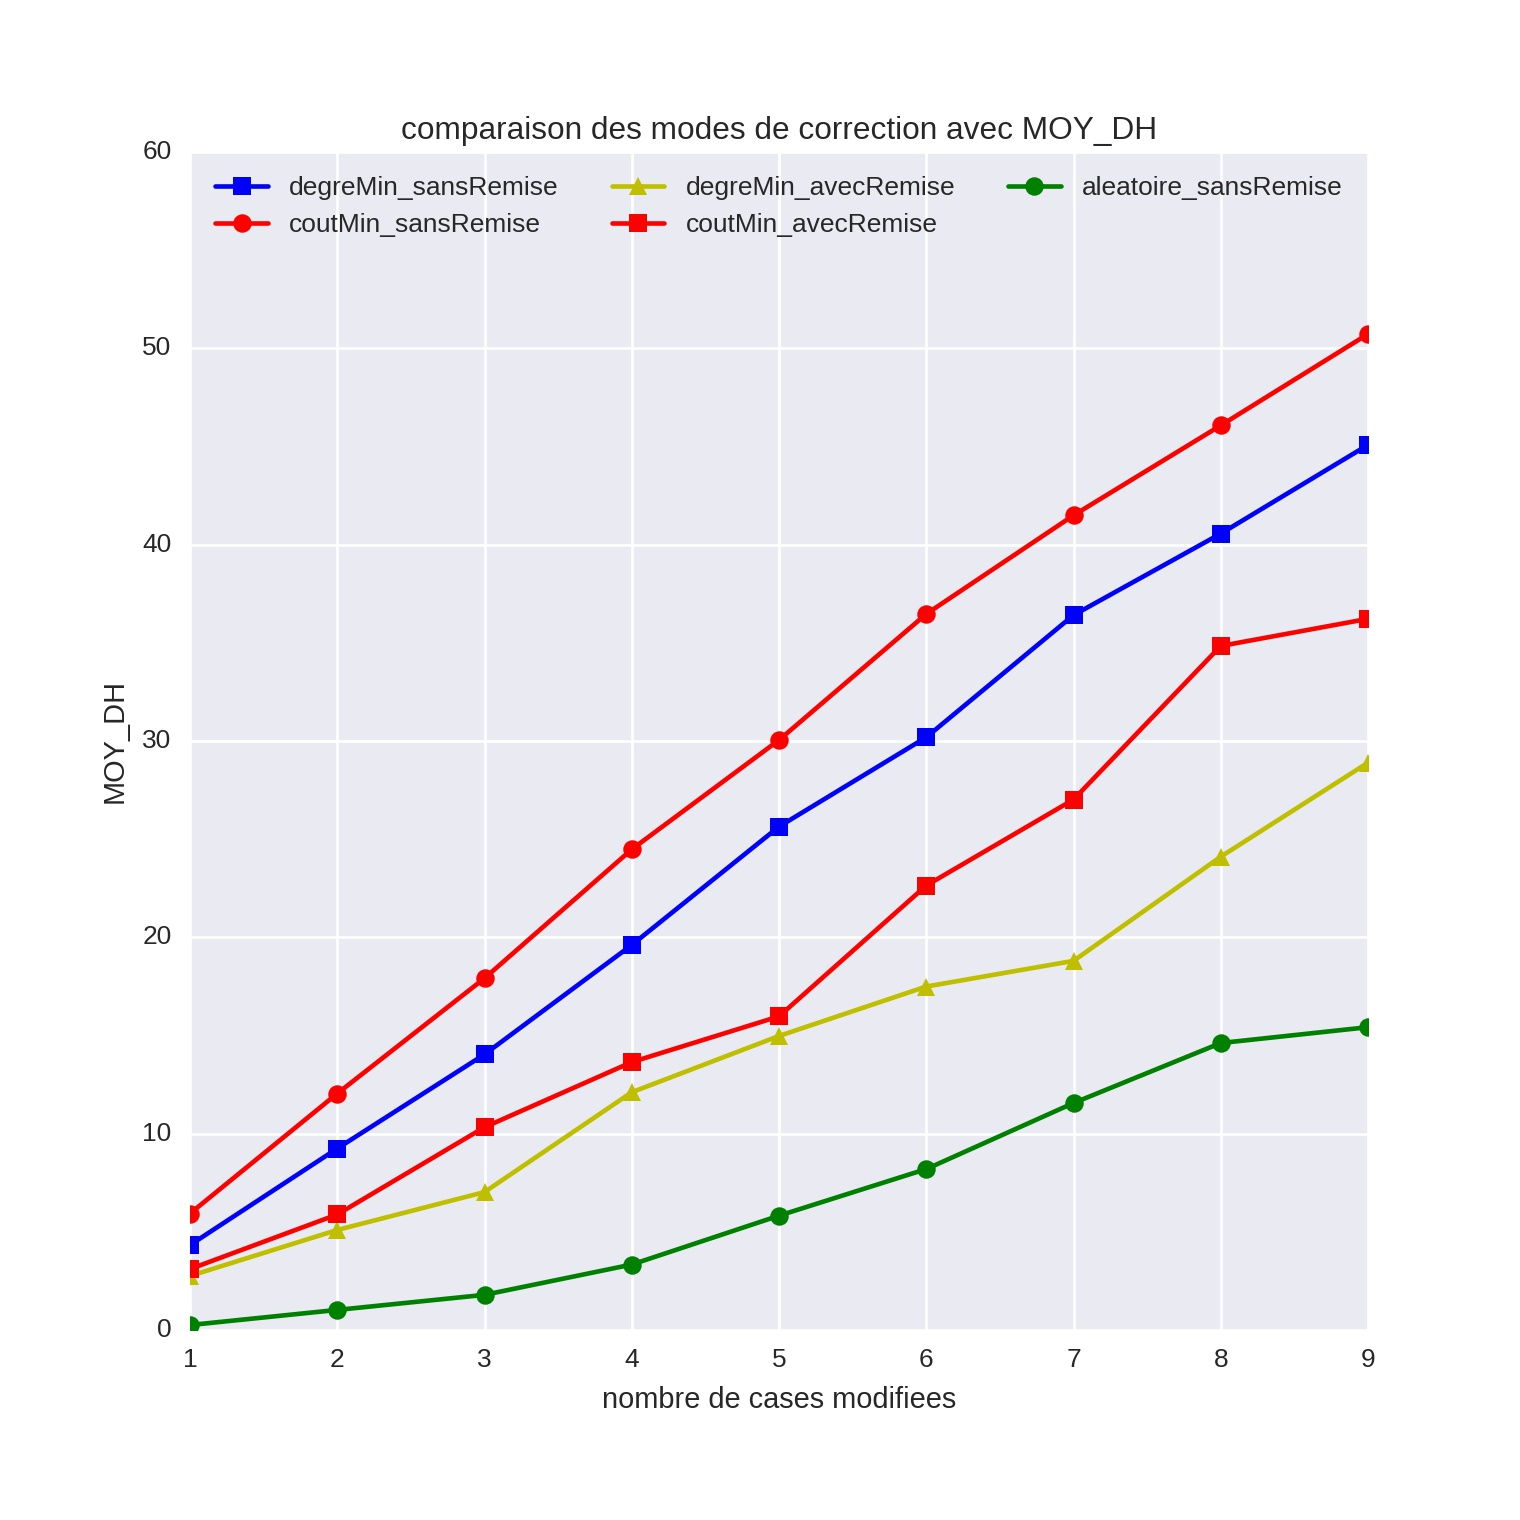
\includegraphics[scale=0.25]{simulation_comparaisonDifferentesMethodes_by_FonctDeCout_unitaire_500G_p_correl_05.jpeg}
\caption{ Comparaison des diff\'erentes approches de correction de sommets pour $k \in \{1,\cdots,9\}$ cases modifi\'ees. 
Les courbes en bleu carr\'e : approche degr\'e minimum sans remise (2a), 
			rouge carr\'ee : approche co\^ut minimum avec remise (1b), 
			rouge rond : approche co\^ut minimum sans remise (2b), 
			vert rond : approche al\'eatoire sans remise (2c) et 
			jaune triangle : approche degr\'e minimum avec remise (1a) 
}
\label{compareDifferentesMethodesCorrectionSommets_fct_cout_normal_p05} 
\end{figure}
\FloatBarrier
% ----------- figure compareDifferentesMethodesCorrectionSommets _fct_cout_normal_p05 ----


Consid\'erons des courbes associ\'ees aux approches $(2b)$, $(2c)$ et $(1b)$. 
En choisissant les nombres de cases modifi\'ees $k \in \{4, 8\}$, nous avons $moy\_DH_{k,p} \in \{4,15\}$ cases pour l'approche $(2c)$, $moy\_DH_{k,p} \in \{13, 36\}$ cases  pour l'approche $(1b)$ et $moy\_DH_{k,p} \in \{25, 46\}$ cases  pour l'approche $(2b)$.
Pour $k=4$ cases modifi\'ees, l'approche $(1b)$  modifie, en moyenne, $9$ cases de plus que l'approche $(2c)$. En revanche, ce nombre moyen de cases modifi\'ees augmente \`a $21$ cases quand $k=8$. 
De m\^eme, l'approche $(2b)$ modifie $12$ cases de plus que l'approche $(1b)$ pour $k=4$ cases modifi\'ees et $10$ cases pour $k=8$ cases.
L'approche  $(2c)$ donne de meilleures r\'esultats par rapport aux approches $(1b)$ et $(2b)$.
\newline


% conclusion
{\bf Conclusion} : l'approche {\em al\'eatoire sans remise} propose de meilleurs r\'esultats que les approches $(2a)$, $(2b)$, $(1a)$ et $(1b)$ parce que les distances de correction sont minimales pour toute valeur de $k$ comme le montre la figure \ref{compareDifferentesMethodesCorrectionSommets_fct_cout_normal_p05}.
Nous retenons, pour la suite,  l'approche {\em al\'eatoire sans remise}  comme l'approche de correction des sommets de $\cal C$, sommets n'appartenant \`a aucune couverture.
%D'autre part, ce r\'esultat a \'et\'e obtenu avec la fonction de co\^ut {\em unitaire}.




		\subsubsection{Influence des cases modifi\'ees et de la fonction de co\^ut}
			\label{influenceFonctionCoutDistributionHamming1}
			% ------------- comparaison_p_correl_s_aleatoire_aucune ----------
\begin{figure}[htb!] 
\centering
% aleatoire aucune = aleatoire unitaire
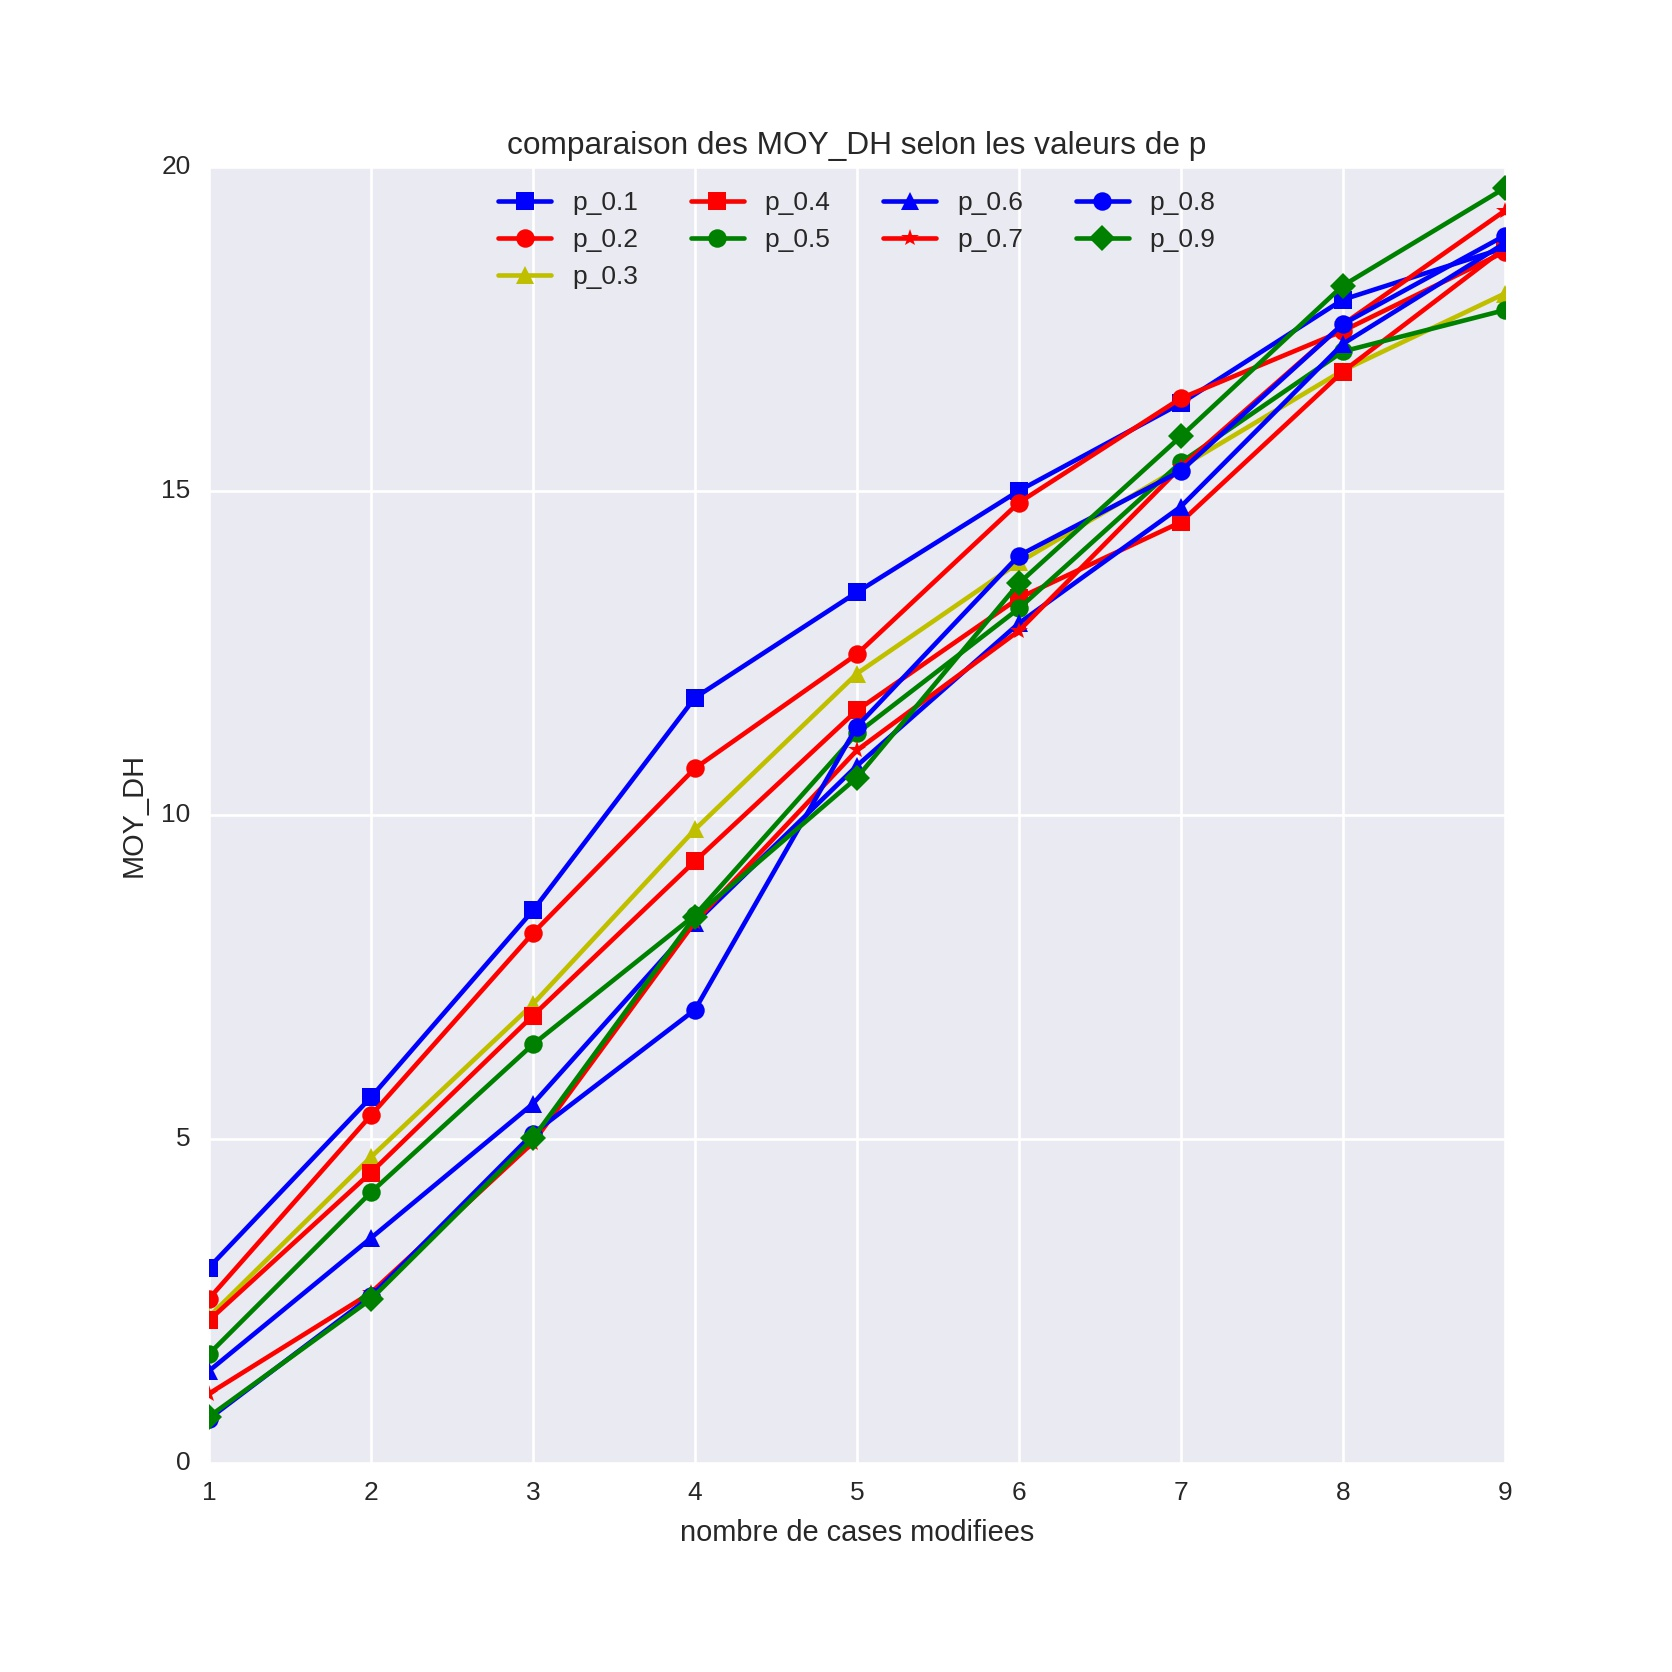
\includegraphics[scale=0.25]{comparaison_p_correl_s_aleatoire_aucune.jpeg}
\caption{ Comparaison des diff\'erentes repartitions des $k \in \{1,\cdots,9\}$ cases fausses positives et fausses n\'egatives avec l'approche {\em al\'eatoire sans remise} et la fonction de co\^ut {\em unitaire}. }
\label{comparaison_p_correl_s_aleatoire_aucune} 
\end{figure}
%\FloatBarrier
% ------------- comparaison_p_correl_s_aleatoire_aucune ----------


Nous mesurons l'influence des fonctions de co\^ut sur nos distances de Hamming.
Pour ce faire, nous appliquons les fonctions de co\^ut {\em unitaire}, {\em ajout} et {\em suppression} (voir tableau \ref{tab:recapApprocheCorrection}) pour en d\'eduire les valeurs de $p$ qui sont favorables \`a l'algorithme de correction c'est-\`a-dire qui minimisent les distances de Hamming.
\newline

Nous consid\'erons d'abord la fonction {\em unitaire}.
La figure \ref{comparaison_p_correl_s_aleatoire_aucune} repr\'esente l'\'evolution des distances de Hamming selon les diff\'erentes valeurs de $p$.  Les courbes de $p$ sont \'eloign\'ees pour $k \le 5$ et au d\'el\`a de  $k > 5$, les courbes se rapprochent. 
En effet, 
pour $k \le 5$, $43.4\%$ des cases {\em fausses n\'egatives} en moyenne sont corrig\'ees pour $p\in \{0.7, 0.9\}$ et pour $p=0.8$, cette moyenne est de $45.5\%$. Quant aux cases {\em fausses positives}, seulement $10\%$ des cases sont corrig\'ees. 
Ces moyennes sont plus \'elev\'ees que celles obtenues avec $p<0.7$.  
En effet, seulement $19.32\%$ des cases {\em fausses positives} et $38\%$ des cases  {\em fausses n\'egatives} sont corrig\'ees avec  $p<0.7$. 
 L'algorithme de correction ajoute beaucoup d'ar\^etes pour $p \ge 0.7$ par rapport \`a $p<0.7$ parce que le nombre de cases {\em fausses n\'egatives} dans la matrice du graphe de corr\'elation est \'elev\'e pour $p<0.7$ sachant que le co\^ut d'ajout  d'une ar\^etes est de $1$.
\newline
De m\^eme, pour $k > 0.5$, $80\%$ des cases erron\'ees sont des cases {\em fausses n\'egatives} apr\`es l'algorithme de correction.  L'algorithme privil\'egie l'ajout  \`a la suppression d'ar\^etes. 
\newline
La fonction {\em unitaire} a peu d'influence sur les variations des distances de Hamming quelque soit les valeurs de $p$.  

% ------------- comparaison_p_correl_s_aleatoire_ajout -----------
\begin{figure}[htb!] 
\centering
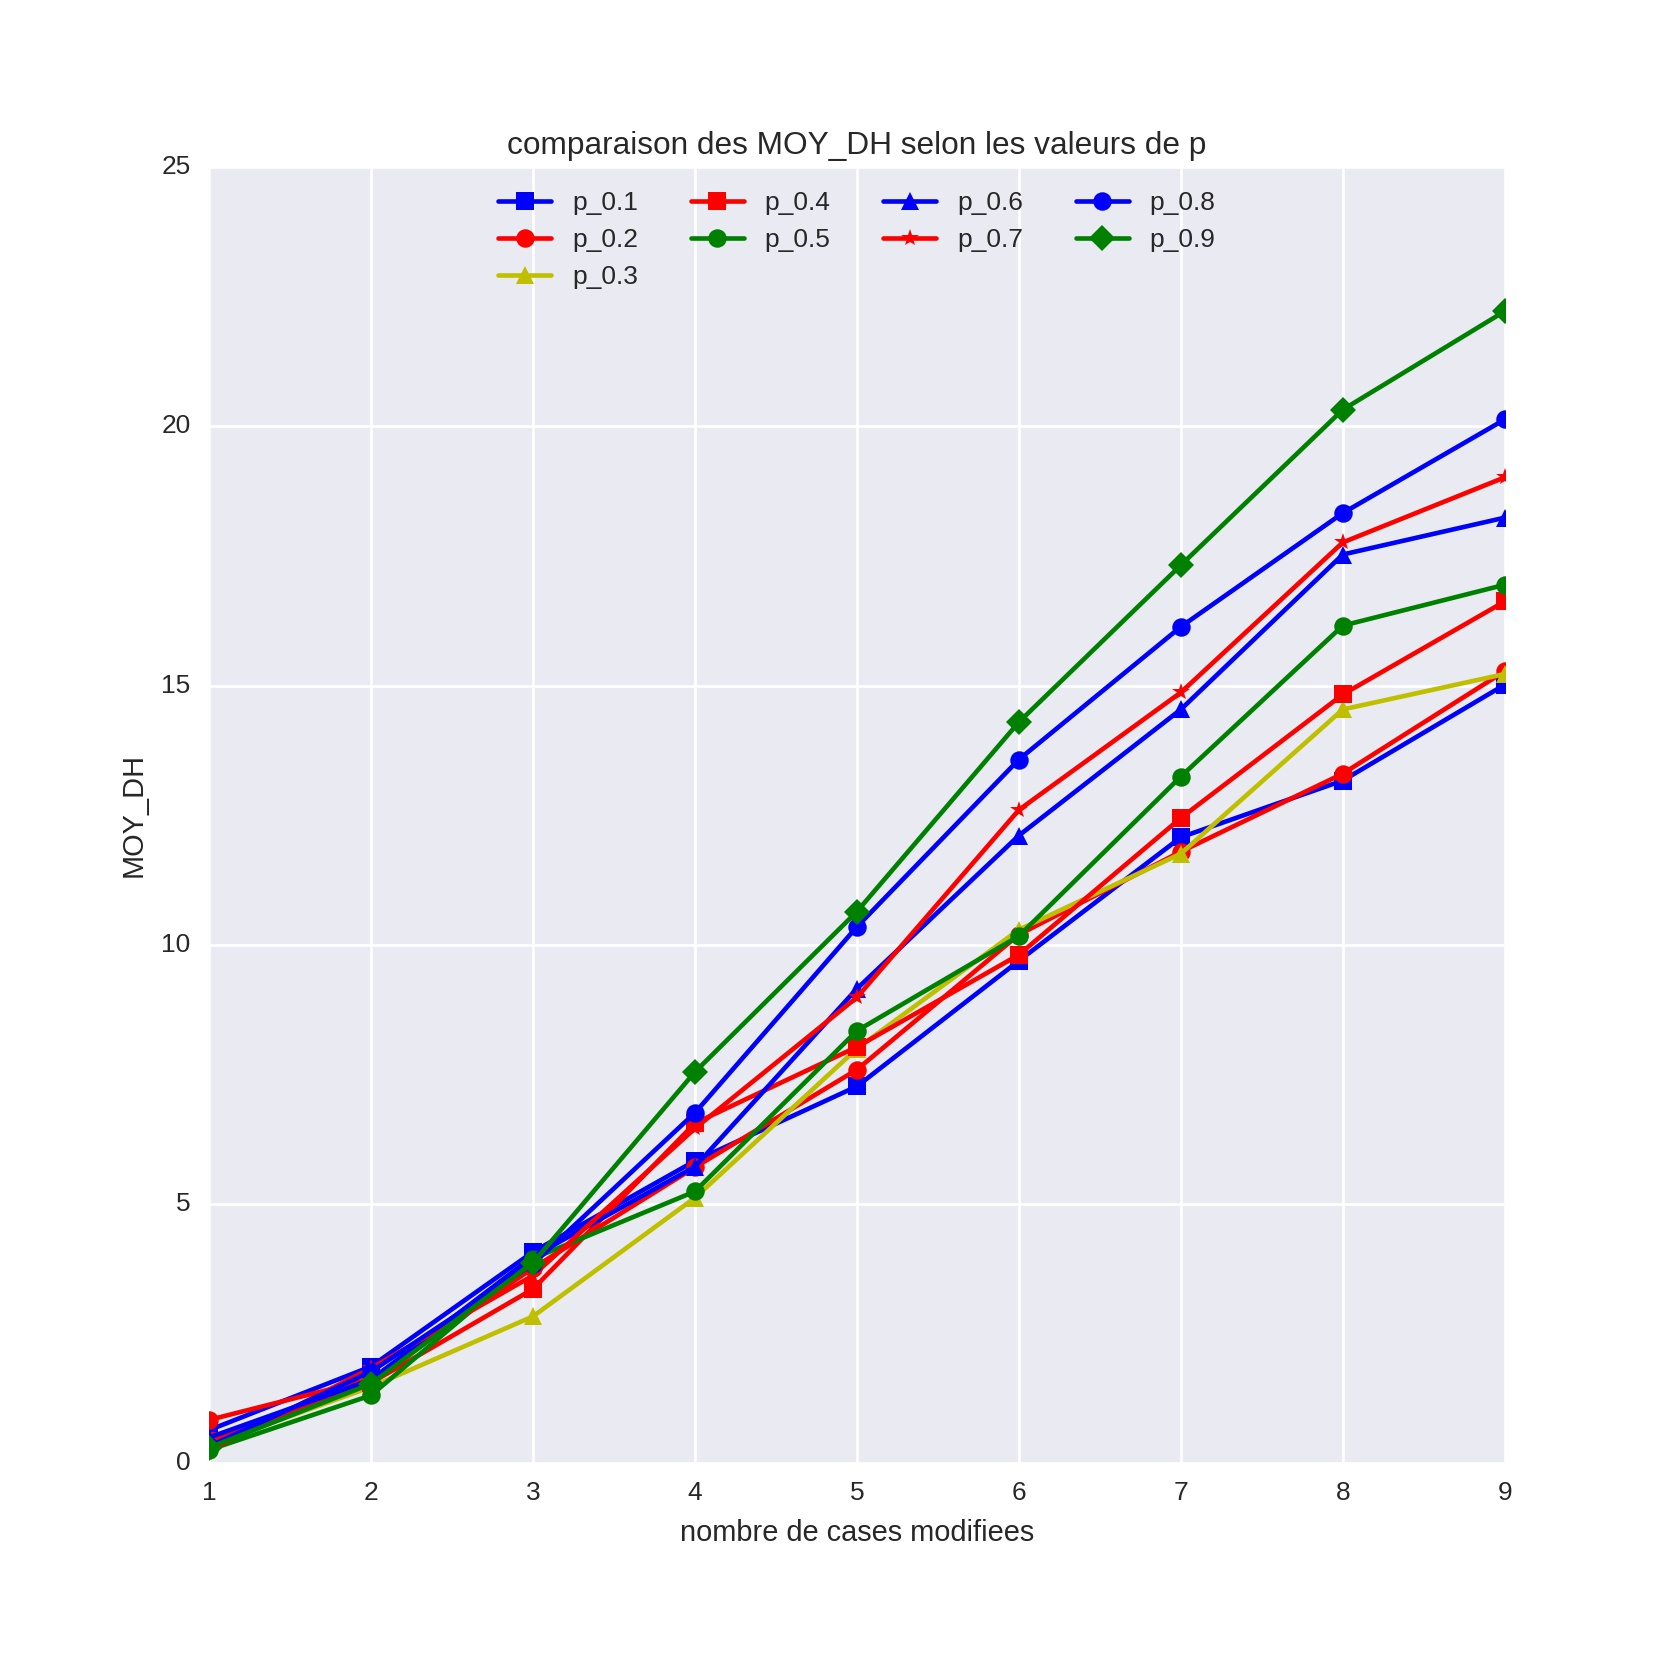
\includegraphics[scale=0.25]{comparaison_p_correl_s_aleatoire_ajout.jpeg}
\caption{ Comparaison des diff\'erentes repartitions des $k \in \{1,\cdots,9\}$ cases fausses positives et fausses n\'egatives avec l'approche {\em al\'eatoire sans remise} et la fonction de co\^ut {\em ajout}.  }
\label{comparaison_p_correl_s_aleatoire_ajout} 
\end{figure}
%\FloatBarrier
% ------------- comparaison_p_correl_s_aleatoire_ajout -----------

La figure \ref{comparaison_p_correl_s_aleatoire_supp} correspond \`a la fonction {\em suppression} et elle a le m\^eme comportement que la fonction {\em unitaire} parce que toutes les courbes divergent quand $k \le 5$ et convergent quand  $k > 5$. Ici nous remarquons aussi que nous avons en moyenne beaucoup de cases {\em fausses n\'egatives} en moyenne \`a la fin de l'algorithme de correction. 
Avec la fonction {\em suppression}, nous constatons que le nombre moyen de cases {\em fausses n\'egatives} \`a la fin de l'algorithme de correction est largement sup\'erieur au nombre de cases {\em fausses n\'egatives} modifi\'ees dans la matrice $M_{k,p,\alpha}$.
Cependant, le nombre de ces cases {\em fausses n\'egatives}  ($39.4\%$ en moyenne) \`a la fin de l'algorithme de correction est inf\'erieur au nombre de cases corrig\'es {\em fausses n\'egatives}  ($47.7\%$ en moyenne) avec la fonction {\em unitaire}. 
Cette baisse provient majoritairement de la position des sommets \`a corriger dans ${\cal C}$. 
En effet, il existe des chaines simples de longueur $2$ entre certains sommets de  ${\cal C}$.  Une ar\^ete de chacune des chaines est supprim\'ee afin que la compression de deux cliques fournisse une nouvelle clique de ${\cal CC}$. Cela fait que les ar\^etes incidentes ont leurs sommets de ${\cal CC}$ et ces ar\^etes sont supprim\'ees une fois sur deux au minimum. 
La fonction {\em suppression} donne le m\^eme r\'esultat que la fonction {\em unitaire}.
%\newline

% ------------- comparaison_p_correl_s_aleatoire_supp  ----------
\begin{figure}[htb!] 
\centering
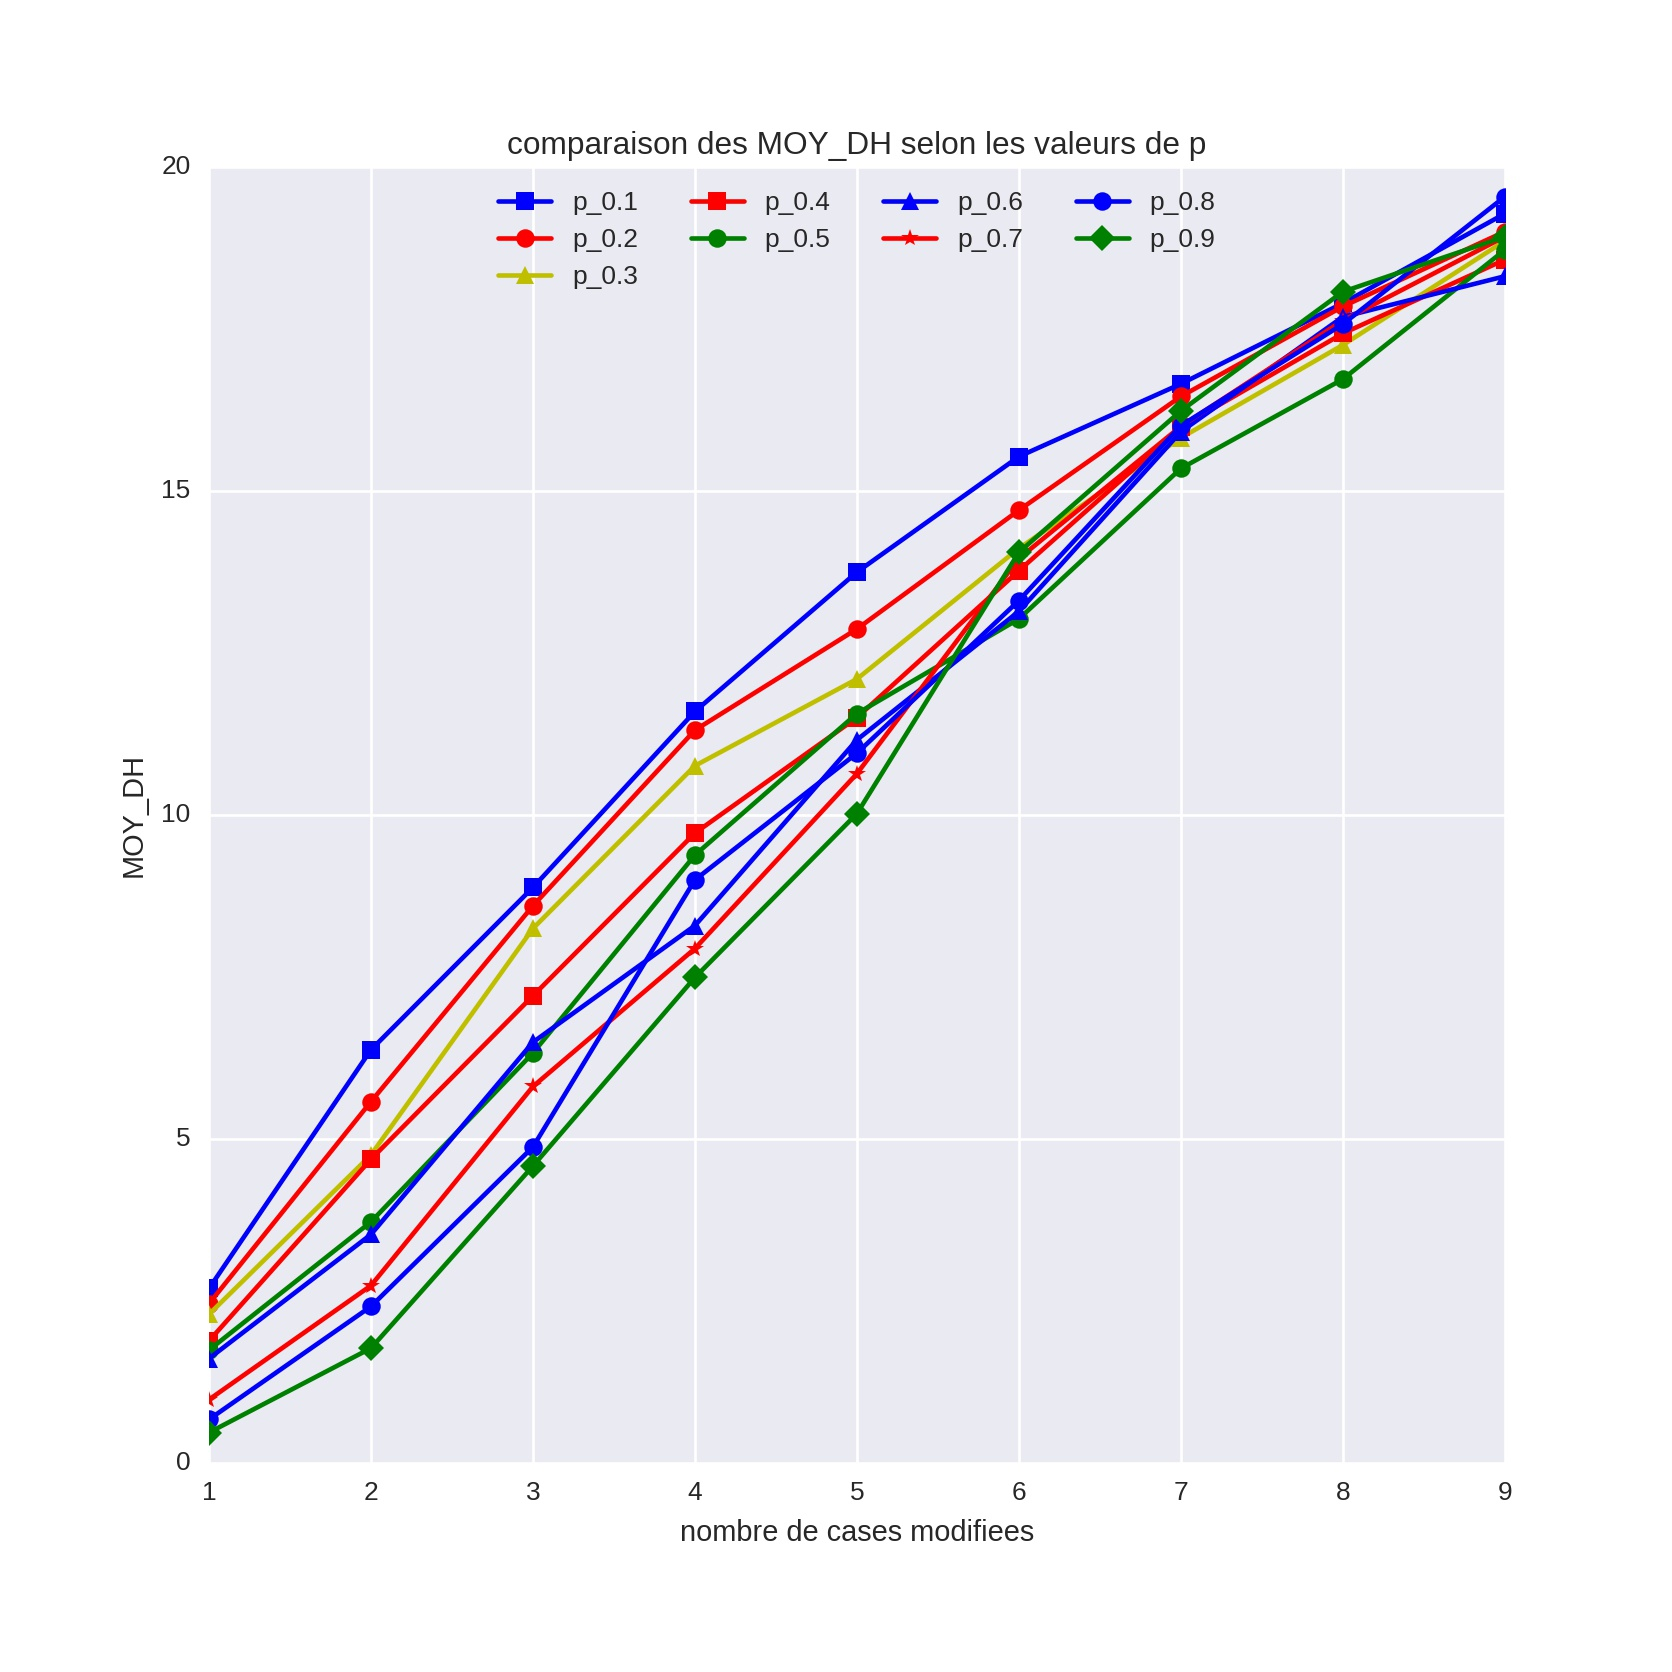
\includegraphics[scale=0.25]{comparaison_p_correl_s_aleatoire_supp.jpeg}
\caption{ Comparaison des diff\'erentes repartitions des $k \in \{1,\cdots,9\}$ cases fausses positives et fausses n\'egatives avec l'approche {\em al\'eatoire sans remise} et la fonction de co\^ut {\em suppression}. }
\label{comparaison_p_correl_s_aleatoire_supp} 
\end{figure}
%\FloatBarrier
% ------------- comparaison_p_correl_s_aleatoire_supp  ----------

Dans la figure \ref{comparaison_p_correl_s_aleatoire_ajout} associ\'ee \`a la fonction {\em ajout}, les courbes divergent quand $k$ est croissant.
En effet, des ar\^etes {\em fausses n\'egatives}  sont ajout\'ees \`a $G_{k,p,\alpha}$ pour $p \ge 0.4$ pendant la correction. Alors les distances $moy\_DH_{k,p}$ augmentent car le nombre de cases  {\em fausses n\'egatives} augmente et aussi plus de  $40\%$ des cases {\em fausses positives} ne sont pas supprim\'ees.  
Par ailleurs, les courbes convergent vers $0$ quand $k \le 4$. La baisse des valeurs moyennes des distances de Hamming est le r\'esultat de la correction des cases modifi\'ees dans $M_{k,p}$. N\'eanmoins, l'algorithme corrige majoritairement des cases {\em fausses n\'egatives} lorsque toutes les cases modifi\'ees ne parviennent pas \`a \^etre corrig\'ees. 
\newline

{\bf Conclusion} : nous ne pouvons pas conclure que les valeurs de $p$ ont une influence sur la correction des $k$ cases modifi\'ees car les fonctions de co\^ut {\em unitaire} et {\em suppression} font converger l'une vers l'autre leurs distances de Hamming avec l'augmentation du nombre de cases modifi\'ees. Toutefois, la fonction de co\^ut {\em ajout} fait diverger nos courbes sans cr\'eer un \'ecart significatif de distances entre ses courbes. 



%
%Consid\'erons $p \in [0,1]$, la variable de repartition des $k$ cases modifi\'ees. 
%$p = 0.1$ signifie que $10\%$ des $k$  cases modifi\'ees ajoutent des ar\^etes au graphe  $G_{k,p, \alpha}$ (cases {\em fausses positives}) et les $90\%$ des cases restantes suppriment des ar\^etes du graphe (cases {\em fausses n\'egatives}). Nous pr\'ecisons \'egalement que la fonction de co\^ut est {\em unitaire}.
%La figure \ref{comparaison_p_correl_s_aleatoire_aucune} r\'esume 
%l'\'evolution des distances de Hamming $moy\_DH$ en fonction des $k \in \{1,\cdots,9\}$ cases modifi\'ees pour diff\'erentes valeurs de $p$. 
%Les courbes sont croissantes et  la courbe de $p = 0.8$ donne les distances de Hamming minimales  \`a partir de $k \le 4 $. Au d\'el\`a de $k > 4$, les courbes se rapprochent les unes des autres et il est difficile de d\'eterminer la valeur $p$ qui fournit la plus petite distance.
%En effet, pour  $k \le 4$, les courbes divergent parce que les cases modifi\'ees ne sont pas corrig\'ees et d'autres cases sont modifi\'ees. Cela augmente l'ensemble de cases ({\em fausses n\'egatives et fausses positives}).
%N\'eammoins, les cases modifi\'ees sont corrig\'ees pour $k > 4$ et cela entraine que les courbes se rapprochent.
%Le probl\`eme de la bonne repartition semble \^etre difficile \`a trouver pour la fonction de cout {\em unitaire}. Nous allons appliquer d'autres fonctions de co\^ut pour d\'eduire une valeur de $p$ acceptable qui minimise les distances de Hamming.
%\newline
%La fonction de co\^ut {\em suppression} a le m\^eme comportement que la fonction {\em unitaire} comme indiqu\'e dans la figure \ref{comparaison_p_correl_s_aleatoire_supp}. La divergence des courbes se produit pour $k \in \{1,\cdots,5\}$ et la courbe de $p = 0.9$ fournit les distances de Hamming minimales (sa courbe est en dessous des autres). \`A partir de $k > 5$, les courbes se rapprochent et la meilleure courbe est  celle de $p = 0.5$. 
%Nous l'expliquons par la modification des cases {\em fausses n\'egatives} pour $p =0.9$ et par  l'ajout d'ar\^etes pour $p = 0.5$.
%\newline
%Dans la figure \ref{comparaison_p_correl_s_aleatoire_ajout} associ\'ee \`a la fonction de co\^ut {\em ajout}, les courbes divergent quand $k$ est croissant.
%En effet, des ar\^etes suppl\'ementaires  sont ajout\'ees \`a $G_{k,p}$ pour $p \ge 0.4$. Les distances $moy\_DH$ augmentent car plus de  $40\%$ des cases {\em fausses positives} ne sont pas supprim\'ees.  
%Par ailleurs, pour $p = 0.1$, la distance de Hamming moyenne est de $1.421,2.305,3.109$ pour $k = 1,2,3$ respectivement et pour $k \ge 4$, cette distance augmente d'environ $1.5 \times k$.
%L'algorithme corrige autour de $20\%$ les cases {\em fausses n\'egatives} et les ar\^etes de la distance de Hamming correspondent majoritairement aux cases {\em fausses positives} modifi\'ees  pendant la phase de correction.
%\newline
%Nous ne pouvons pas conclure que la repartition des $k$ cases modifi\'ees de $M_{LG}$ a un impact sur la correction des sommets $noeud \in {\cal C}$ car les fonctions de co\^ut {\em unitaire} et {\em suppression} font converger nos distances de Hamming avec l'augmentation du nombre de cases modifi\'ees. Toutefois, la fonction de co\^ut {\em ajout} fait diverger nos courbes sans cr\'eer un \'ecart significatif de distances entre ses courbes.  


% ----- partir a envoyer 



%% comparaison de p_correl sur la methode de permutation aleatoire
%%% ---- pas encore REPROGRAMMER -- utiliser la fonction de cout unitaire
%\begin{figure}[htb!] 
%\centering
%% meilleur probabilite p parmi les [0.0, 0.1, 0.2, ...., 1.0]
%% a changer par des chemins relatifs
%%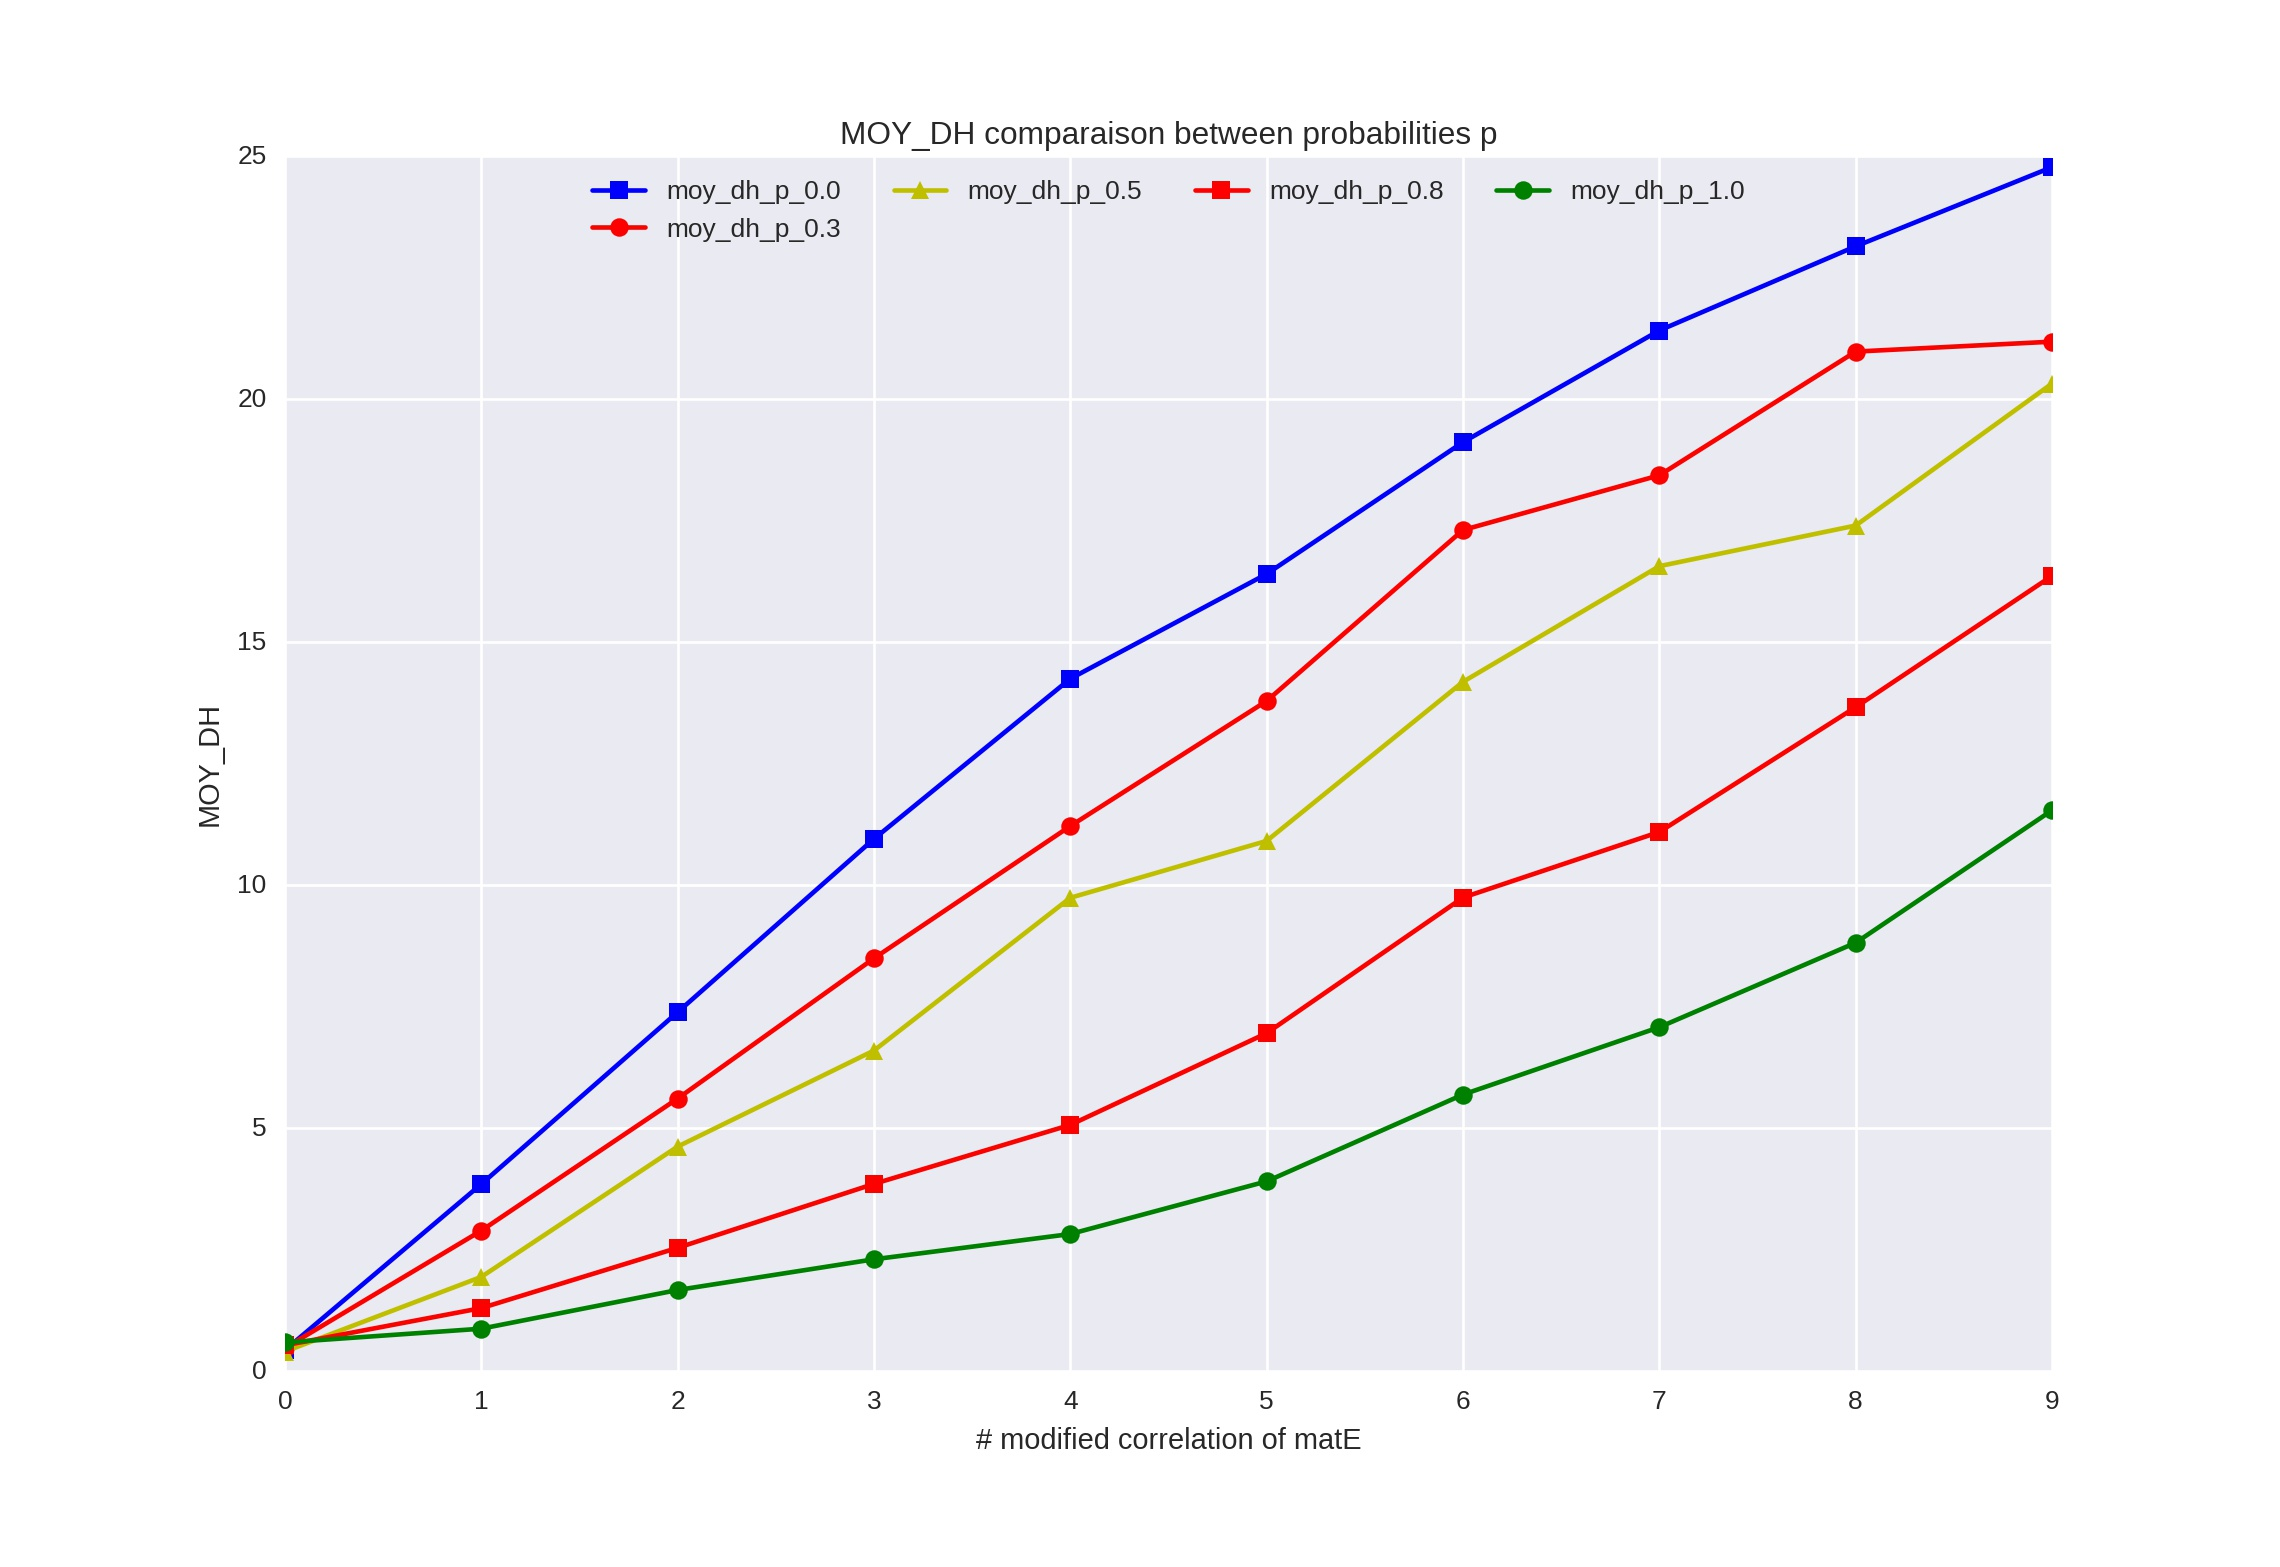
\includegraphics[scale=0.25]{permut_aleatoire_coutMin_degreMin_fct_cout_normal_500G/aleatoire/courbes/comparaison_probabilities_p_00_10_moy_dh_aleatoire_p_10.jpeg}
%%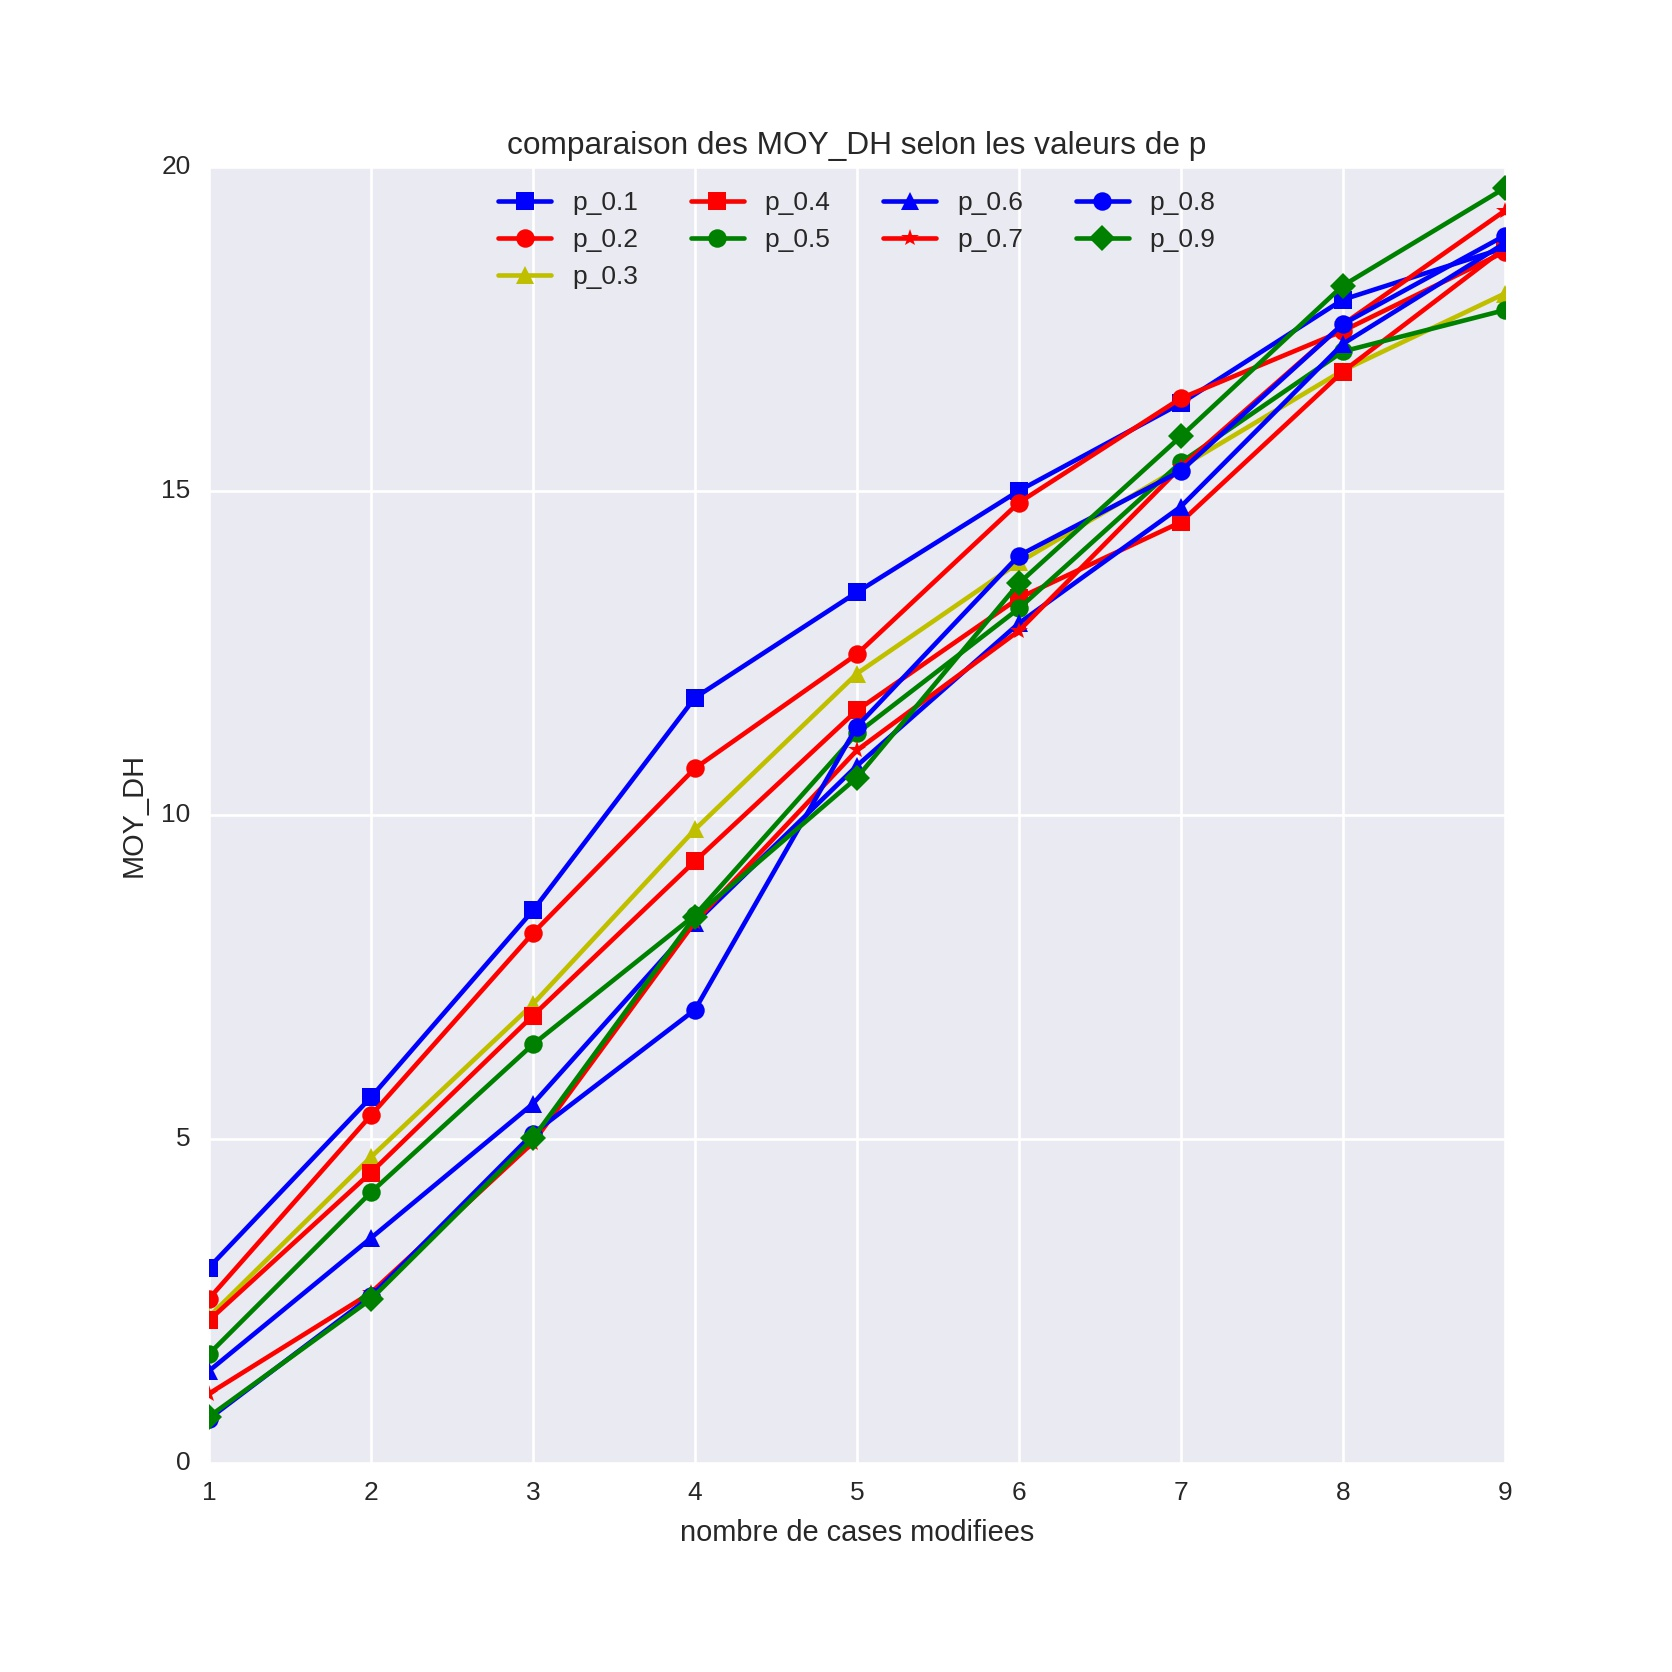
\includegraphics[scale=0.25]{comparaison_p_correl_s_aleatoire_aucune.jpeg}
%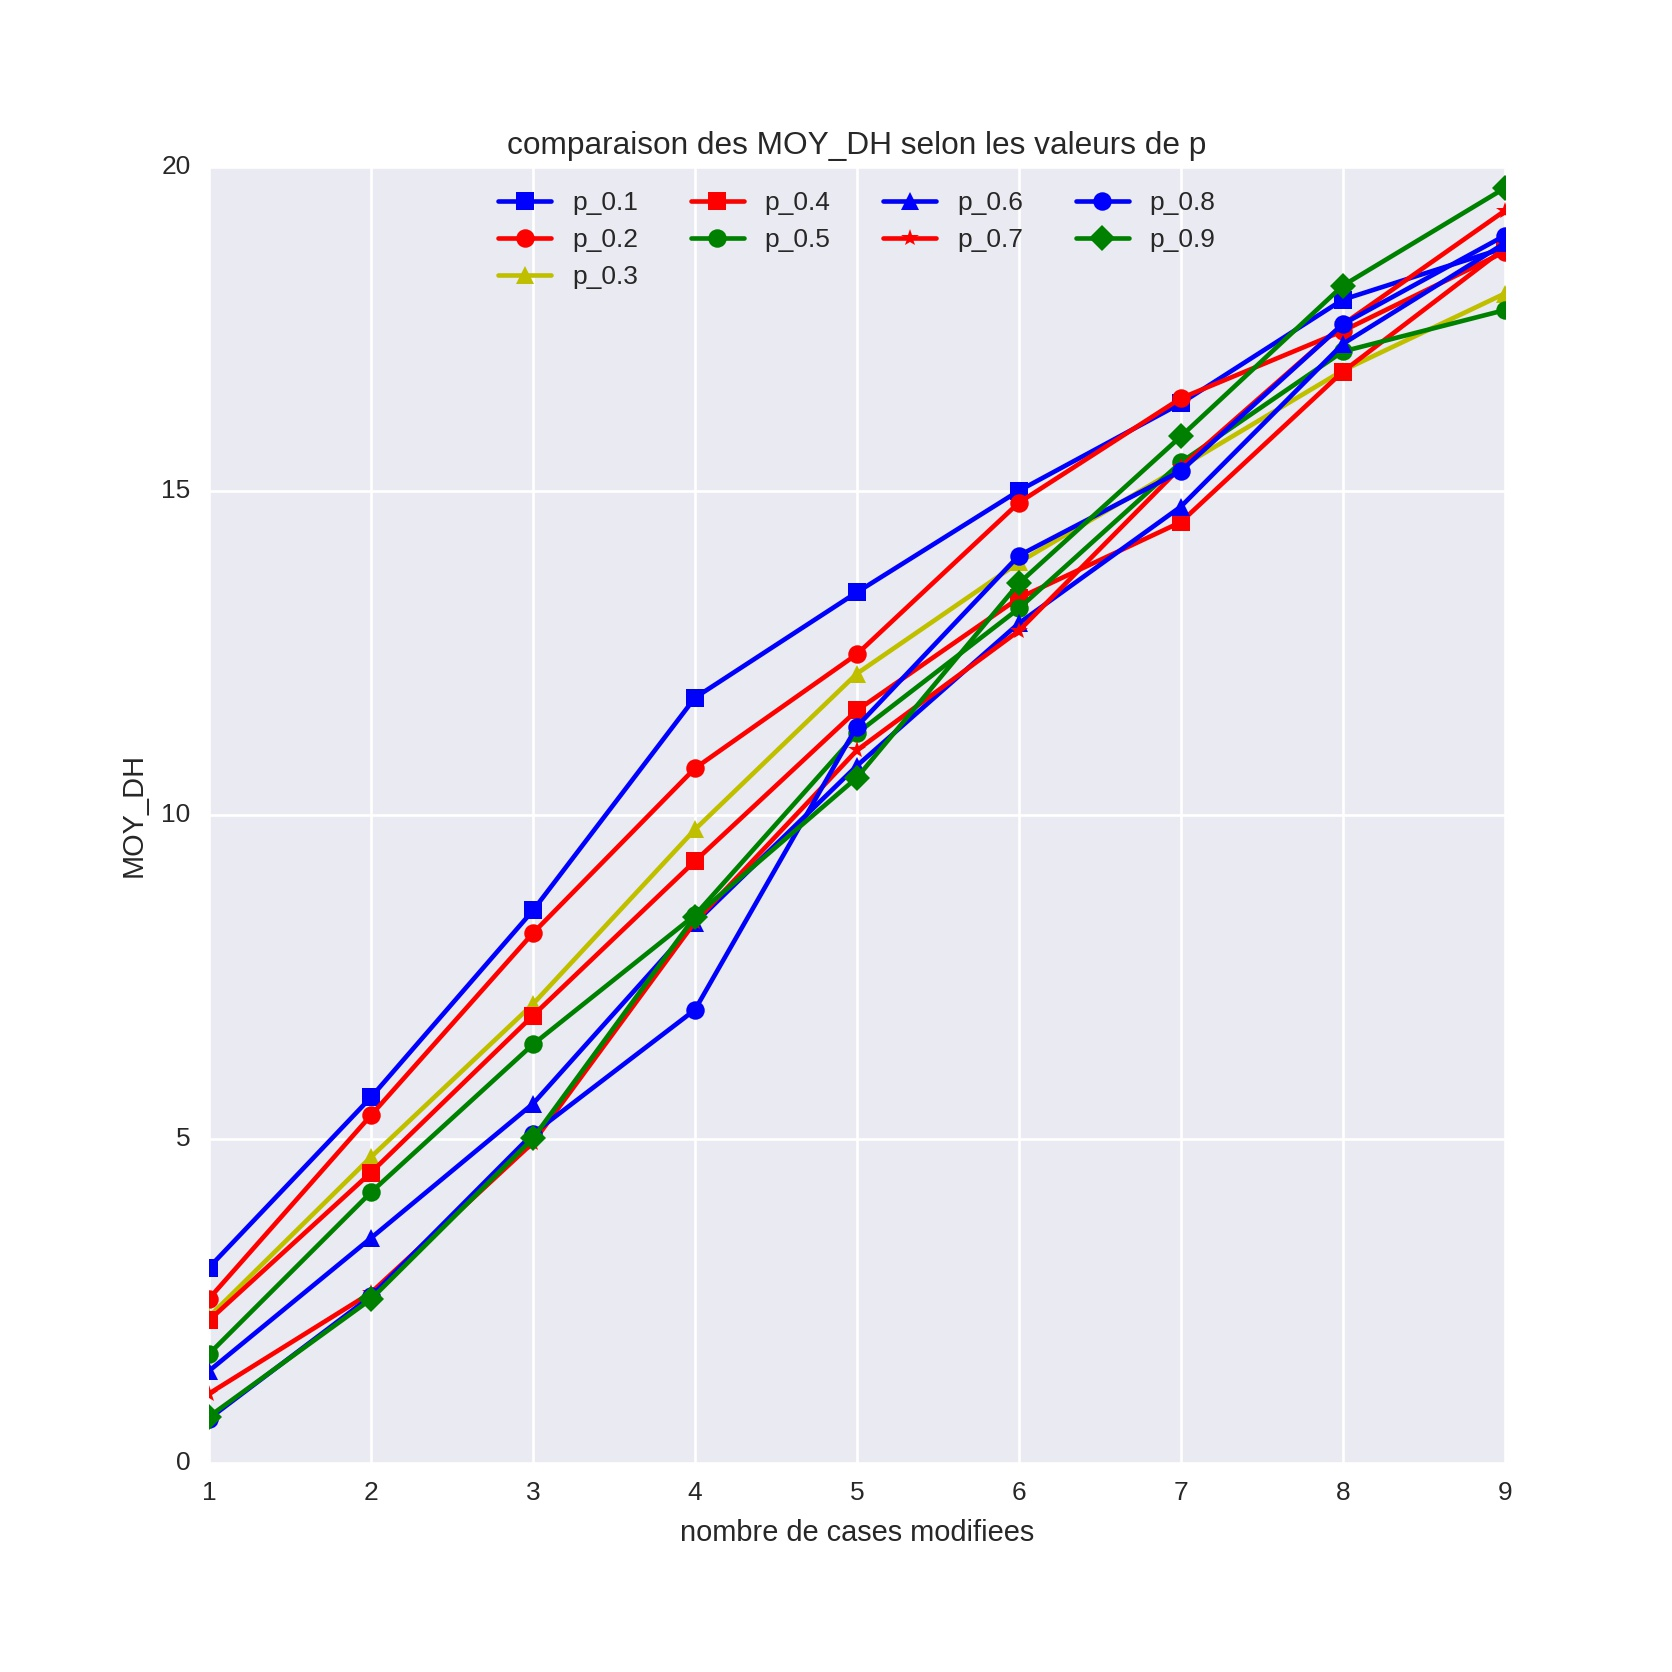
\includegraphics[scale=0.25]{comparaison_p_correl_s_aleatoire_aucune.jpeg}
%\caption{ Comparaison des diff\'erentes probabilit\'es d'ajout $k \in [1,9]$ de corr\'elations fausses positives et fausses n\'egatives sur la m\'ethode de permutation al\'eatoire }
%\label{comparaison_p_correl_s_aleatoire_aucune} 
%\end{figure}
%%% ---- pas encore REPROGRAMMER
%Consid\'erons la variable $p\_correl \in [0,1]$. 
%$p\_correl = 0.1$ signifie que $10\%$ des $k$  cases modifi\'ees ajoutent des ar\^etes au graphe  $G_{k,p\_correl, \alpha}$ (erreurs {\em fausses positives}) et les $90\%$ des cases restantes suppriment des ar\^etes du graphe (erreurs {\em fausses n\'egatives}). Nous pr\'ecisons \'egalement que  l'ajout et la suppression d'ar\^etes ont le m\^eme co\^ut de traitement c'est-\`a-dire $1$.
%La figure \ref{comparaison_p_correl_s_aleatoire_aucune} r\'esume 
%l'\'evolution des distances de Hamming $moy\_DH$ en fonction des $k \in [1,9]$ cases modifi\'ees pour diff\'erentes valeurs de $p\_correl$. 
%Les courbes sont croissantes et nous constatons que pour $k \le 4 $, la courbe de $p\_correl = 0.8$ donne les distances de Hamming minimales. Au d\'el\`a de $k > 4$, les courbes se rapprochent les unes des autres et il est difficile de determiner la valeur $p\_correl$ qui fournit la plus petite distance.
%En effet, La parit\'e de co\^uts n'impacte pas les d\'ecisions de l'algorithme de correction qui aura tendance \`a ajouter et supprimer des ar\^etes. Pour $k \le 4$, les courbes divergent parce que les cases modifi\'ees ne sont pas corrig\'ees et des erreurs sont ajout\'ees dans chaque ensemble d'erreurs ({\em fausses n\'egatives et fausses positives}). Ces erreurs sont soit l'ajout d'ar\^etes  dans les erreurs {\em fausses positives} ou soit la suppression d'ar\^etes dans les  erreurs {\em fausses n\'egatives}. Cependant, les courbes se rapprochent pour $k > 4$ car l'algorithme ajoute et supprime plusieurs fois les m\^emes ar\^etes. 
%%De m\^eme, le taux d'erreurs {\em vrai n\'egatives} et {\em fausses positives} restent stables dans l'ensemble    =====> A complter apres la courbe.
%Il nous est impossible d'affirmer la bonne repartition des $k$ cases dans le  cas {\em priorit\'e aucune}.
%\newline
%En changeant la {priorit\'e aucune} aux {\em priorit\'es ajout ou suppression}, parvenons nous \`a deduire une valeur de $p\_correl$ acceptable c'est-\`a-dire qui minimise les distances de Hamming? 
%% reste priorite suppression 
%\newline
%La {\em priorit\'e suppression} a le m\^eme comportement que la {\em priorit\'e aucune} comme indiqu\'e dans la figure \ref{comparaison_p_correl_s_aleatoire_supp}. La divergence des courbes se produit pour $k \in [1,5]$ avec la courbe de $p\_correl = 0.9$ fournissant les distance de Hamming minimales (sa courbe est en dessous des autres). \`A partir de $k > 5$, les courbes convergent et la meilleure courbe \'est  celle de $p\_correl = 0.5$. 
%\begin{figure}[htb!] 
%\centering
%%\includegraphics[scale=0.25]{comparaison_taux_vrai_negatifs_corriges_p_correl_s_aleatoire_supp.jpeg}
%\caption{ Taux d'erreurs fausses negatives corrig\'ees pour $k \in [1,9]$ cases modif\'ees et une m\'ethode de corr\'elation al\'eatoire avec la priorit\'e suppression}
%\label{comparaison_taux_vrai_negatifs_corriges_p_correl_s_aleatoire_supp} 
%\end{figure}
%Nous l'expliquons par la suppression des erreurs {\em fausses n\'egatives} (voir figures \ref{comparaison_taux_vrai_negatifs_corriges_p_correl_s_aleatoire_supp}) pour $p_correl =0.9$ et par  la correction des ar\^etes pour $p\_correl = 0.5$
%
%
%Dans la figure \ref{comparaison_p_correl_s_ajout} associ\'ee \`a la {\em priorit\'e ajout}, Les courbes divergent quand $k$ est croissant. {\bf Pourquoi?} En effet, l'algorithme de correction a tendance \`a ajouter des ar\^etes dans le voisinage des sommets \`a corriger. Cela entraine des ar\^etes suppl\'ementaires qui augmentent la distance de Hamming pour les valeurs de $p\_correl \ge 0.4$, \'etant donn\'ee que plus de $40\%$ des erreurs {\em fausses positives} ne sont pas supprim\'ees.  
%Par ailleurs, pour $p\_correl = 0.1$, la distance de Hamming moyenne est de $1.421,2.305,3.109$ pour $k = 1,2,3$ respectivement et pour $k \ge 4$, cette distance augmente d'environ $1.5 * k$. L'algorithme corrige autour de $20\%$ les erreurs {\em fausses n\'egatives} et les ar\^etes diff\'erentes de la distance de Hamming correspondent aux erreurs {\em fausses positives} et majoritairement aux ar\^etes ajout\'ees de l'algorithme.
%Toutefois le taux d'ar\^etes corrig\'ees dans les erreurs {\em fausses n\'egatives} est tr\^es bas comme le montre la figure \ref{comparaison_taux_vrai_negatifs_corriges_p_correl_s_aleatoire_ajout}. 
%\begin{figure}[htb!] 
%\centering
%%\includegraphics[scale=0.25]{comparaison_taux_vrai_negatifs_corriges_p_correl_s_aleatoire_ajout.jpeg}
%\caption{ Taux d'erreurs fausses negatives corrig\'ees pour $k \in [1,9]$ cases modif\'ees et une m\'ethode de corr\'elation al\'eatoire avec la priorit\'e ajout}
%\label{comparaison_taux_vrai_negatifs_corriges_p_correl_s_aleatoire_ajout} 
%\end{figure}
%\newline
%Nous ne pouvons pas conclure que la repartition des $k$ cases modifi\'ees de $M_{LG}$ est un impact sur la correction des sommets $\in sommets\_1$ car notre algorithme a un defaut celui d'ajouter des ar\^etes et aussi le taux d'erreurs {\em fausses negatives} corrig\'es est tr\`es faible.
%%Cette valeur $p\_correl = 0.1$ est relativement meilleure par rapport aux autres valeurs parce qu'elle ajoute moins d'ar\^etes par rapport aux 
%
%
%
%%Nous constatons que les algorithmes donnent de meilleurs r\'esultats pour $p\_correl = 1$ et de mauvais r\'esultats pour $p\_correl = 0$. 
%%En d'autres termes, lorsque nous  ajoutons que des erreurs {\em fausses n\'egatives} i.e $p\_correl  = 0$ dans la matrice $matE$, les algorithmes  proposent, dans la majorit\'e des cas, un line graphe $LG_k$ dont ces erreurs de corr\'elation sont supprim\'ees.




		\subsubsection{Relation entre la distance de Hamming et la distance de correction}
			 \label{relationMoyDHmoyDC}
 
Nous allons calculer les corr\'elations entre les distances de correction et de Hamming en se basant sur le  graphe $G$, son line-graphe $LG$ et le line-graphe $LG_{k,p, \alpha}$ obtenus par notre couple d'algorithmes.
Notre objectif est de montrer la relation entre ces deux distances.
\newline
Consid\'erons les distances de correction et de Hamming obtenues par l'approche {\em al\'eatoire sans remise}, la variable $p = 0.5$ et la fonction de co\^ut {\em unitaire} (voir tableau \ref{tab:recapApprocheCorrection}).

% ----------------------------- figure  correlation distance hamming distance correlation -------------------- 
 \begin{figure}[htb!] 
\centering
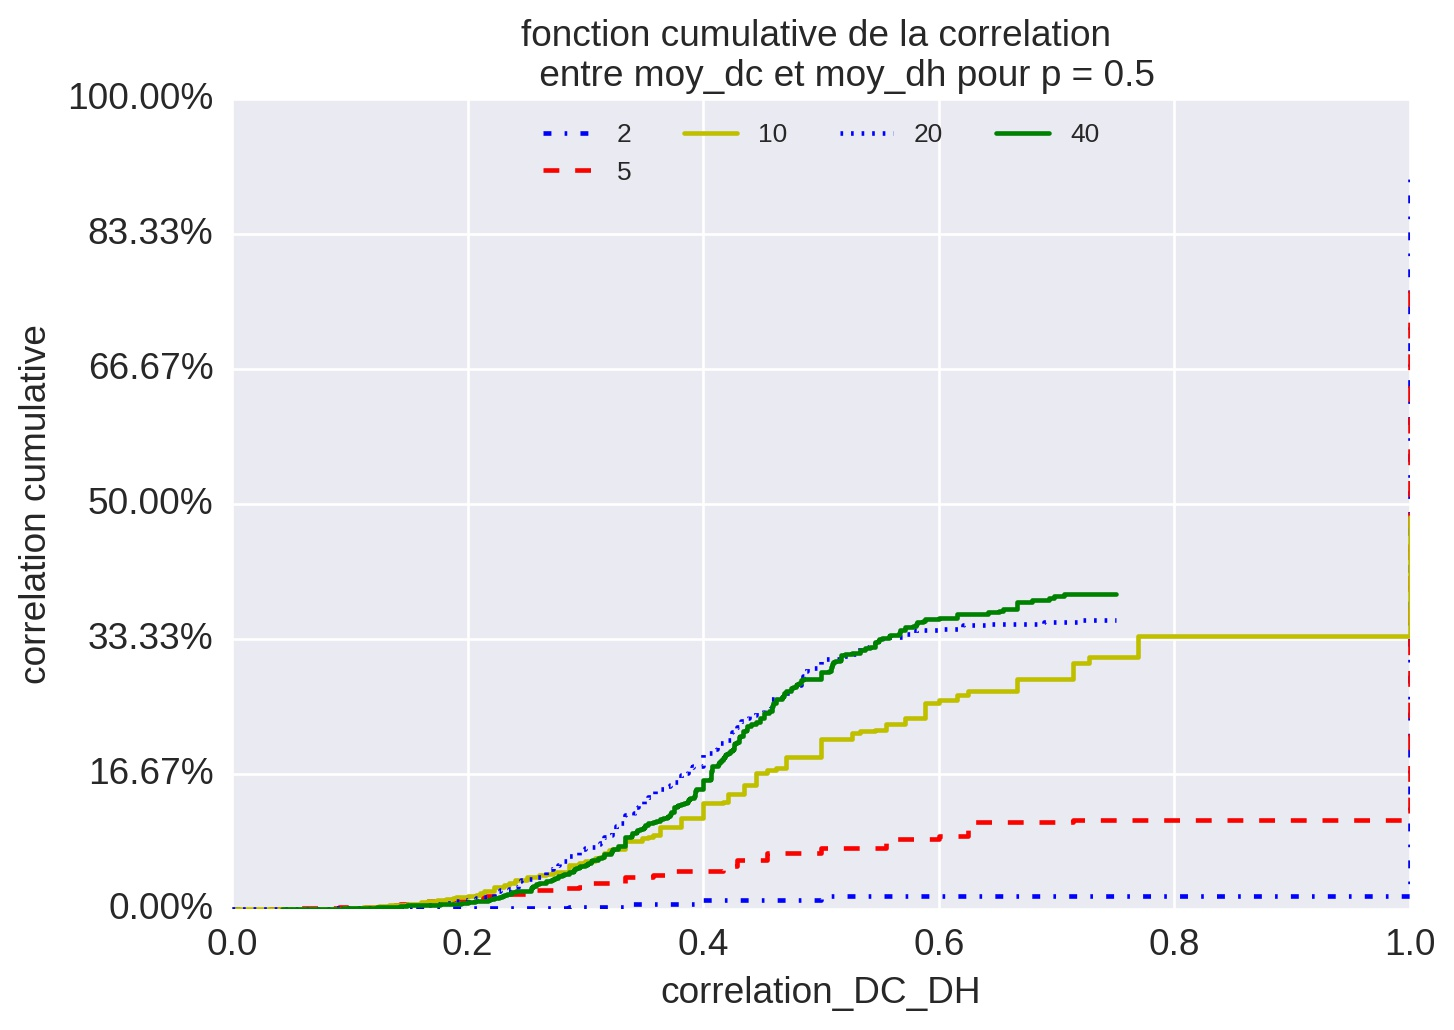
\includegraphics[scale=0.35]{correlation_dh_dl_p_05.jpeg}
\caption{ La corr\'elation de la distance de correction versus la distance de Hamming pour $k$ cases modifi\'ees et $p = 0.5$ }
\label{dh_vs_dc_p_05} 
\end{figure}
\FloatBarrier
% ----------------------------- figure  correlation distance hamming distance correlation -------------------- 

Nous calculons la corr\'elation entre les distances de correction et de Hamming avec la formule \ref{correlation_correction_hamming}.
%\begin{multline}
\begin{equation}
	corr_{k,p,\alpha} =  \frac{ | moy\_DC_{k, p,\alpha} - moy\_DH_{k,p, \alpha} | }{ max(moy\_DC_{k, p,\alpha},  moy\_DH_{k, p, \alpha}) };
	\\
	corr_{k,p} = \sum_{\alpha = 1}^{5}corr_{k,p,\alpha} ;
	\\ \newline
	F_k (x,p) = P(corr_{k,p} < x ) 
\label{correlation_correction_hamming}
\end{equation}
%\end{multline}
avec $x \in [0,1]$ une valeur de corr\'elation et $k$ le nombre de cases modifi\'ees. 
La fonction $corr_{k,p,\alpha}$ retourne l'\'ecart entre ces deux distances sous la forme de valeurs probabilistes. 
Ainsi $corr_{k,p,\alpha} = 1$ indique qu'il n'existe aucune corr\'elation entre les distances de correction et de Hamming c'est-\`a-dire que $moy\_DC_{k,p,\alpha} = k$ et $moy\_DH_{k,p,\alpha} = 0$.
De m\^eme, $corr_{k,p} = 0$ indique que ces distances sont identiques c'est-\`a-dire $ moy\_DC_{k, p, \alpha} = moy\_DH_{k,p, \alpha}$. En moyenne, $moy\_DH_{k,p, \alpha}$ tend vers $k$ cases modifi\'ees. 
\newline

La figure \ref{dh_vs_dc_p_05} repr\'esente la fonction de repartition $F_k$ dans laquelle nous avons, en abscisse, la corr\'elation entre les distances et, en ordonn\'e, le pourcentage de graphes dont la corr\'elation moyenne $corr_{k,p}$ est inf\'erieure \`a $x \in [0,1]$. 
%si $F_k$ a une courbe d'\'equation $y = 100$  ====> intuition pour la definition F_k
Si $corr_{k,p,\alpha} = 0$ alors les matrices de $LG_{k,p,\alpha}$ et $LG$ sont diff\'erentes de $k$ cases quand $k < 6$ ($LG_{k,p,\alpha} \neq LG$).
Si $corr_{k,p,\alpha} = 1$ alors le line-graphe $LG_{k, p, \alpha}$ est le line-graphe du graphe $G$ ($LG_{k, p, \alpha} = LG$) et $F_k(1) \approx 0$. 
La corr\'elation $corr_{k,p} = 1$ est sa valeur maximale. 
Ce cas est illustr\'e dans la figure \ref{dh_vs_dc_p_05} par les courbes de $k \in \{2,5\}$. 
Par exemple $F_5(1) \approx 10\%$ signifie que nous avons $70-10=60\%$ des line-graphes $LG_k$ qui ont le m\^eme ensemble d'ar\^etes que les line-graphes $LG$ ($70\%$ est le pourcentage de corr\'elations \'egales \`a $1$ $|corr_{5,p} = 1 | = 70\%$ ).
\newline
En revanche, une valeur de $F_k(1)$ tr\`es \'elev\'ee signifie que le nombre $x$ de  $corr_{k,p} = 1$ est tr\`es faible. Ce nombre $x$ implique une corr\'elation tr\`es forte entre les distances de correction et de Hamming.
C'est l'observation faite avec les courbes de $k \in \{10,20,40\}$ de la figure \ref{dh_vs_dc_p_05} dans lesquelles nous avons une  croissance continue en fonction de l'augmentation des valeurs de corr\'elations.
\newline
Nous subdivisons nos courbes en deux cat\'egories:
\begin{itemize}
	\item Celles pour lesquelles il y a une corr\'elation entre les distances de correction et de Hamming (courbes de $k \in \{10,20,40\}$).
	\item Celles pour lesquelles il y a  aucune corr\'elation entre ces distances parce que   $LG = LG_{k,p}$ (courbes de $k \in \{2,5\}$). 
\end{itemize}


{\bf Conclusion} :
il existe de fortes corr\'elations entre les distances de correction et de Hamming lorsque $k \ge 10$. Dans ce cas, nous pouvons utiliser la distance de correction pour calculer les \'ecarts de cases modifi\'ees pendant l'algorithme de correction.
Dans le cas o\`u $k \le 5$, les distances de correction inf\'erieures ou \'egales \`a $5$ cases proposent le line-graphe $LG$ et ces distance entrainent une corr\'elation proche de $0$.
Pour  $k \in \{6,7,8,9\}$, les valeurs de $corr_{k,p}$ avoisinent $0.5$. Ces valeurs sont faibles et nous ne pouvons rien conclure.
Ainsi, pour juger de la qualit\'e de notre algorithme de correction en l'absence de la distance de Hamming, la distance de correction est alors une bonne m\'etrique.

	\subsection{Conclusion de l'exp\'erimention 1}	
		
%----- conclusion 
Les performances de notre couple d'algorithmes ont \'et\'e test\'ees sur des graphes non orient\'es sans circuits qui repr\'esentent la topologie de r\'eseaux \'electriques. Nous avons construit les line-graphes de ces graphes et avons modifi\'e $k$ cases dans les matrices des line-graphes. Les cases modifi\'ees sont reparties en deux ensembles (cases {\em fausses positives} et {\em fausses n\'egatives}) selon la variable $p \in [0,1]$.
L'analyse des performances compare les distances de correction et de Hamming en fonction du nombre de cases modifi\'ees selon $5$ approches de correction et $3$ fonctions de co\^ut (voir tableau \ref{tab:recapApprocheCorrection}). 
Nous concluons que l'approche {\em al\'eatoire sans remise} donne de meilleurs r\'esultats lorsque le nombre $k$ de cases modifi\'ees est faible ($k\le 5$). La distance line est alors major\'ee par la distance de correction.  Le probl\`eme {\em Proxi-Line} a une solution mais elle n'est pas optimale.
En revanche, au-del\`a de $k > 5$, il est alors difficile de d\'eterminer une borne sup\'erieure \`a la distance line car l'algorithme de correction  modifie des cases n'\'etant pas contenues dans les $k$ cases modifi\'ees pr\'ealablement. 
Par ailleurs, nous avons montr\'e que la distance de correction peut \^etre utilis\'ee comme une m\'etrique pour connaitre le nombre de cases modifi\'ees dans la matrice d'un graphe \`a condition que cette distance soit sup\'erieure \`a $10$ ar\^etes. 
Enfin, les fonctions de co\^ut ont peu d'influence sur les distances de correction pendant la phase de correction.

%----- conclusion


%---------------------------------------------------------------------------
%------- 		experimentation 2 	---------------------
%---------------------------------------------------------------------------
\section{Exp\'erimentation 2 : Ajout de probabilit\'e dans la matrice du line-graphe}

Notre seconde exp\'erimentation a le m\^eme but que la premi\`ere sauf qu'ici la modification des cases est faite \`a partir de valeurs de seuils appliqu\'ees \`a des matrices de corr\'elation. Les valeurs de ces matrices sont d\'efinies selon la distribution des valeurs de corr\'elation d'un r\'eseau r\'eel, celui du datacenter {\em Champlan}.
\newline
Notre but est de d\'eterminer la valeur de seuil qui minimise les distances de correction et de Hamming obtenues avec l'approche {\em al\'eatoire sans remise} (tableau \ref{tab:recapApprocheCorrection}). 
\newline
Nous d\'ecrivons tout d'abord l'affectation des valeurs de corr\'elation aux cases de la matrice du line-graphe. Ensuite nous pr\'esentons les diff\'erentes \'etapes de notre exp\'erimentation et enfin nous analysons les r\'esultats obtenus.
	\subsection{Affectation de probabilit\'es aux cases de la matrice $M_{LG}$}
		\label{affectationValeursProbabilites}
		%---------------- distribution_0_1_metrique_wil_shapelets_P_len4950 ------------------
\begin{figure}[htb!] 
\centering
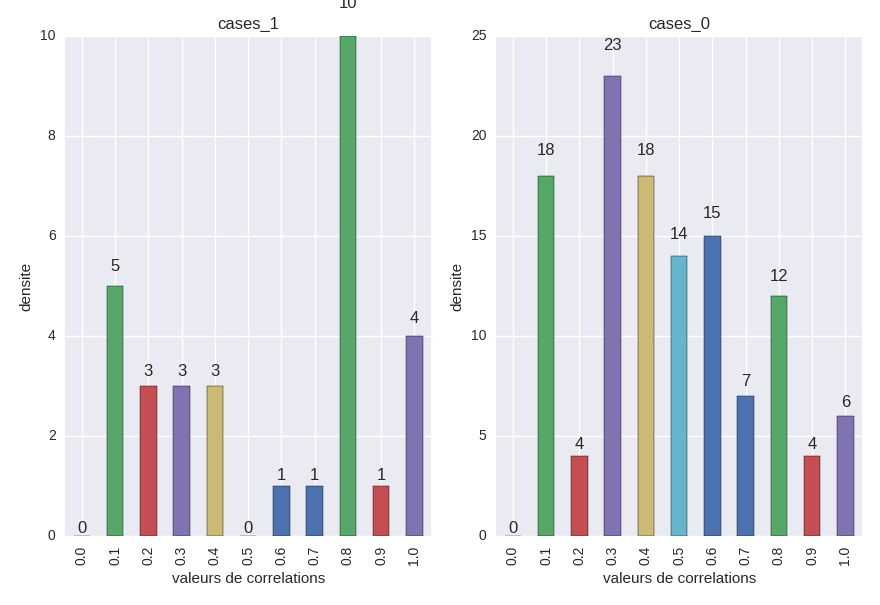
\includegraphics[width=500pt,height=250pt]{distribution_0_1_metrique_wil_shapelets_P_len4950.jpeg}
\caption{ Distribution des valeurs de corr\'elation de $M_c$ selon les cases \`a $0$ (\`a gauche) et \`a $1$ (\`a droite) de $M_{LG}$. La corr\'elation \`a $0.1$ d\'esigne  les valeurs de corr\'elation comprises entre $0.10$ et $0.199$. }
\label{distribution_0_1_metrique_wil_shapelets_P_len4950} 
\end{figure}
% \FloatBarrier
%---------------- distribution_0_1_metrique_wil_shapelets_P_len4950 ------------------


Soient la matrice $M_{LG}$ d'adjacence du line-graphe $LG$ du DAG non orient\'e de {\em Champlan} et $M_c$ sa matrice de corr\'elation obtenue avec la {\em distance de Pearson}.
 La distribution de valeurs de $M_c$ est repr\'esent\'ee par la figure \ref{distribution_0_1_metrique_wil_shapelets_P_len4950}. Le graphique \`a gauche de la figure \ref{distribution_0_1_metrique_wil_shapelets_P_len4950}  est la distribution des valeurs de $M_c$ selon les cases \`a $1$ dans $M_{LG}$ et le graphique \`a droite est celui des cases \`a $0$ dans $M_{LG}$. 
 Par exemple, la valeur de corr\'elation $0.1$ d\'esigne toutes les valeurs appartenant \`a $[0.1, 0.2[$. 
% En d'autres termes, ces distributions sont les celles des valeurs des cases {\em vrai n\'egatives} et {\em vrai positives}.
\newline
La densit\'e des  corr\'elations est d\'ecroissante pour les cases \`a $0$ quand les valeurs de corr\'elation tendent vers $1$. De m\^eme, cette densit\'e est croissante pour les cases \`a $1$ quand les corrections tendent vers $1$. La matrice $M_c$ contient des cases \'erron\'ees et ces cases ont une influence sur le calcul des valeurs de corr\'elation. C'est pourquoi les distributions ne sont pas lin\'eairement croissantes ou d\'ecroissantes.
Nous d\'ecidons, avec nos constatations, que la g\'en\'eration des distributions des valeurs de corr\'elation des cases \`a $0$ et $1$ suivent des lois normales asym\'etriques.
\newline

Nous  g\'en\'erons des valeurs de corr\'elation qui sont similaires \`a la distribution conjectur\'ee des valeurs de corr\'elation  du graphe de {\em Champlan}. Nous supposons que les valeurs de corr\'elation des cases \`a $0$ de $M_{LG}$ suivent la loi asym\'etrique de param\`etre $\alpha = 5$ et les valeurs de corr\'elation  des cases \`a $1$ de $M_{LG}$ suivent  cette m\^eme loi avec $\alpha = -5$ comme illustr\'e dans la figure \ref{distributionsCases01avecCoefficientAsymetries}. 
%---------------- distributionsCases01avecCoefficientAsymetries ------------------
\begin{figure}[htb!] 
\centering
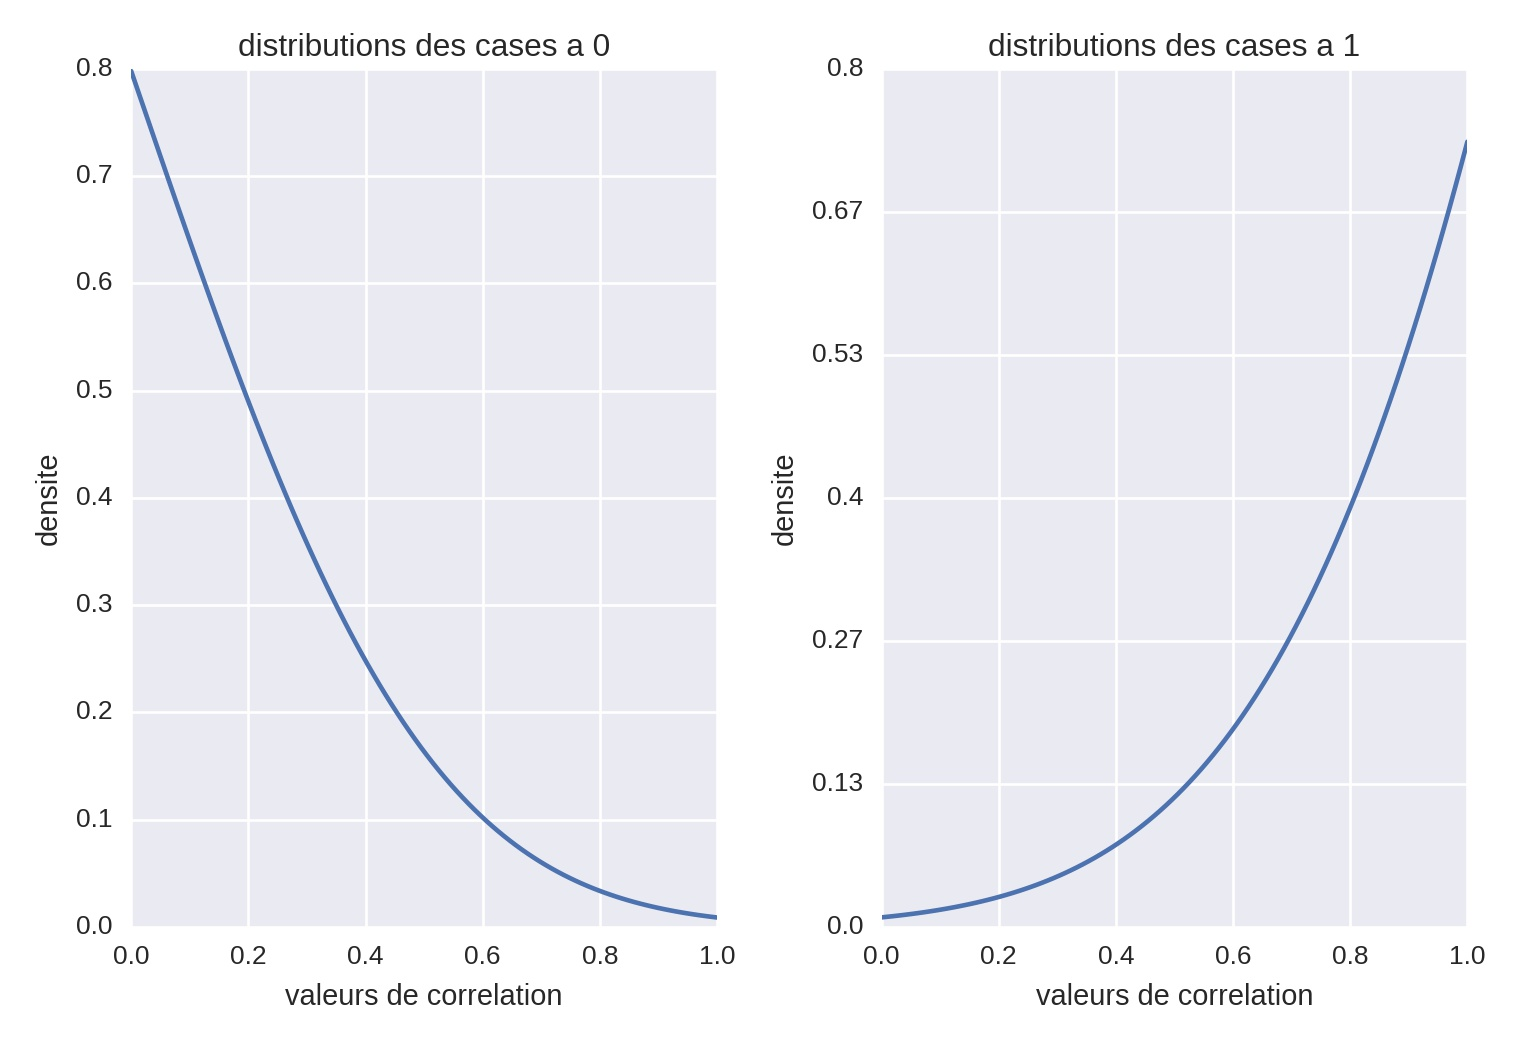
\includegraphics[width=500pt,height=250pt]{distributionsCases01avecCoefficientAsymetries.jpeg}
\caption{ Distribution des cases \`a $0$ et \`a $1$. \`A gauche : loi asym\'etrique de coefficient d'asym\'etrie $\alpha = 5$ pour les cases \`a $0$.  \`A droite : loi asym\'etrique de coefficient d'asym\'etrie $\alpha = -5$ pour les cases \`a $1$.}
\label{distributionsCases01avecCoefficientAsymetries} 
\end{figure}
% \FloatBarrier
%---------------- distributionsCases01avecCoefficientAsymetries ------------------
\newline

Soient 
$n_0$ la cardinalit\'e de l'ensemble des cases \`a $0$  de $M_{LG}$ et $n_1$ la cardinalit\'e de l'ensemble des cases \`a $1$ de $M_{LG}$.
Pour obtenir des valeurs de corr\'elation de $M_c$, nous g\'en\'erons  des valeurs r\'eelles $val$ appartenant \`a $[0,1]$ selon la loi asym\'etrique de coefficient $\alpha = 5$. Nous divisons l'intervalle $ [0,1]$ en $10$ sous-intervalles. Chaque sous-intervalle est not\'e  $]x_i,x_{i+1}]$ avec $x_i$ une valeur de corr\'elation et $i \in [0, 9]$. Nous calculons la densit\'e de chaque sous-intervalle et l'ensemble des densit\'es forme un histogramme qui suit une loi asym\'etrique.
Nous calculons la fonction de repartition $P$ de chaque densit\'e de telle sorte que 
$$
\forall x_i, x_{i+1}, P(X \le x_i) \le P(X \le x_{i+1}) ~~ et ~~ P(X \le x_{10}) = 1.
$$
\newline
Pour chaque case \`a $0$, nous tirons al\'eatoirement $n_0$ nombres r\'eels compris entre $0$ et $1$ uniformement. Si un nombre appartient \`a $]P(X \le x_i), P(X \le x_{i+1}) ]$ alors sa valeur de corr\'elation est $x_{i+1}$. Nous r\'ep\'etons les m\^emes \'etapes pour les cases \`a $1$ en g\'en\'erant les valeurs $val$ avec une loi asym\'etrique de coefficient $\alpha = -5$.
Nous obtenons la matrice de corr\'elation $M_c$ du line-graphe $LG$. Une distribution des valeurs de corr\'elation est repr\'esent\'ee par la figure \ref{distribution01} dans laquelle nous avons $189$ cases \`a $0$ et $111$ cases \`a $1$ dans $LG$.
%---------------- distribution01 ------------------
\begin{figure}[htb!] 
\centering
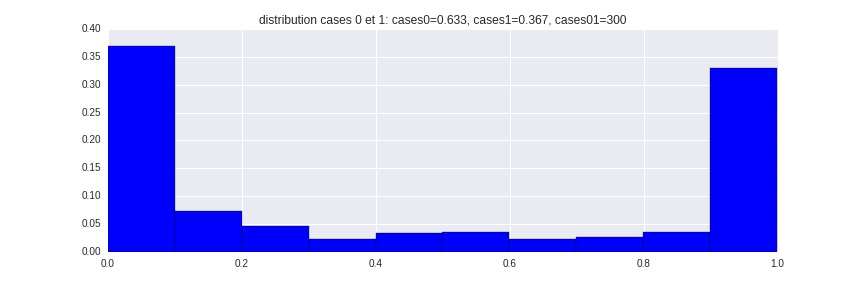
\includegraphics[width=550pt,height=250pt]{distribution01.jpeg}
\caption{ Un exemple de la distribution des valeurs de corr\'elations g\'en\'er\'ees. $63\%$ des cases sont des cases \`a 0 et $37\%$ sont des cases \`a $1$ dans $LG$.}
\label{distribution01} 
\end{figure}
% \FloatBarrier
%---------------- distribution01 ------------------


	\subsection{G\'en\'eration du graphe de corr\'elation }
		\label{experimentation2GenerationMatriceProbabiliteAvecSeuil}
		Nous allons d\'eterminer la matrice d'adjacence du graphe de corr\'elation \`a partir des valeurs de $M_c$.
\newline 
Soit $s = \{ 0.1, \cdots, 0.9\}$, une valeur de seuil choisie.
Nous construisons la matrice $M_s$  selon les r\`egles suivantes : 
\begin{itemize}
\item Si $M_c[i,j] \ge s$ alors $M_s[i,j] = 1$.
\item Si $M_c[i,j] < s$ alors $M_s[i,j] = 0$.
\end{itemize}
La matrice $M_s$ est la matrice d'adjacence du graphe $G_s$  dit {\em graphe de corr\'elation}. Ces cases peuvent contenir des cases erron\'ees. Ces cases erron\'ees proviennent de la s\'election du seuil $s$ et de la g\'en\'eration de valeurs de corr\'elation pour les cases \`a $0$ et \`a $1$ du line-graphe $LG$. En effet ,
\begin{itemize}
	\item Si $M_s [i,j] = M_{LG} [i,j] = 0$ alors $M_{s} [i,j]$ est dit {\em vrai n\'egatif}. 
	\item Si $M_s [i,j] = M_{LG} [i,j] = 1$ alors $M_{s} [i,j]$ est dit {\em vrai positif}. 
	\item Si $M_s [i,j] = 0$ et $M_{LG} [i,j] = 1$ alors $M_{s} [i,j]$ est dit {\em faux n\'egatif}.
	\item Si $M_s [i,j] = 1$ et $M_{LG} [i,j] = 0$ alors $M_{s} [i,j]$ est dit {\em faux positif}.
\end{itemize}
Un exemple de distributions des cases erron\'ees selon les valeurs de seuils est pr\'esent\'e dans la figure \ref{distrib_relationAdjacence_seuils}. 
%---------------- distributionsCases01avecCoefficientAsymetries ------------------
\begin{figure}[htb!] 
\centering
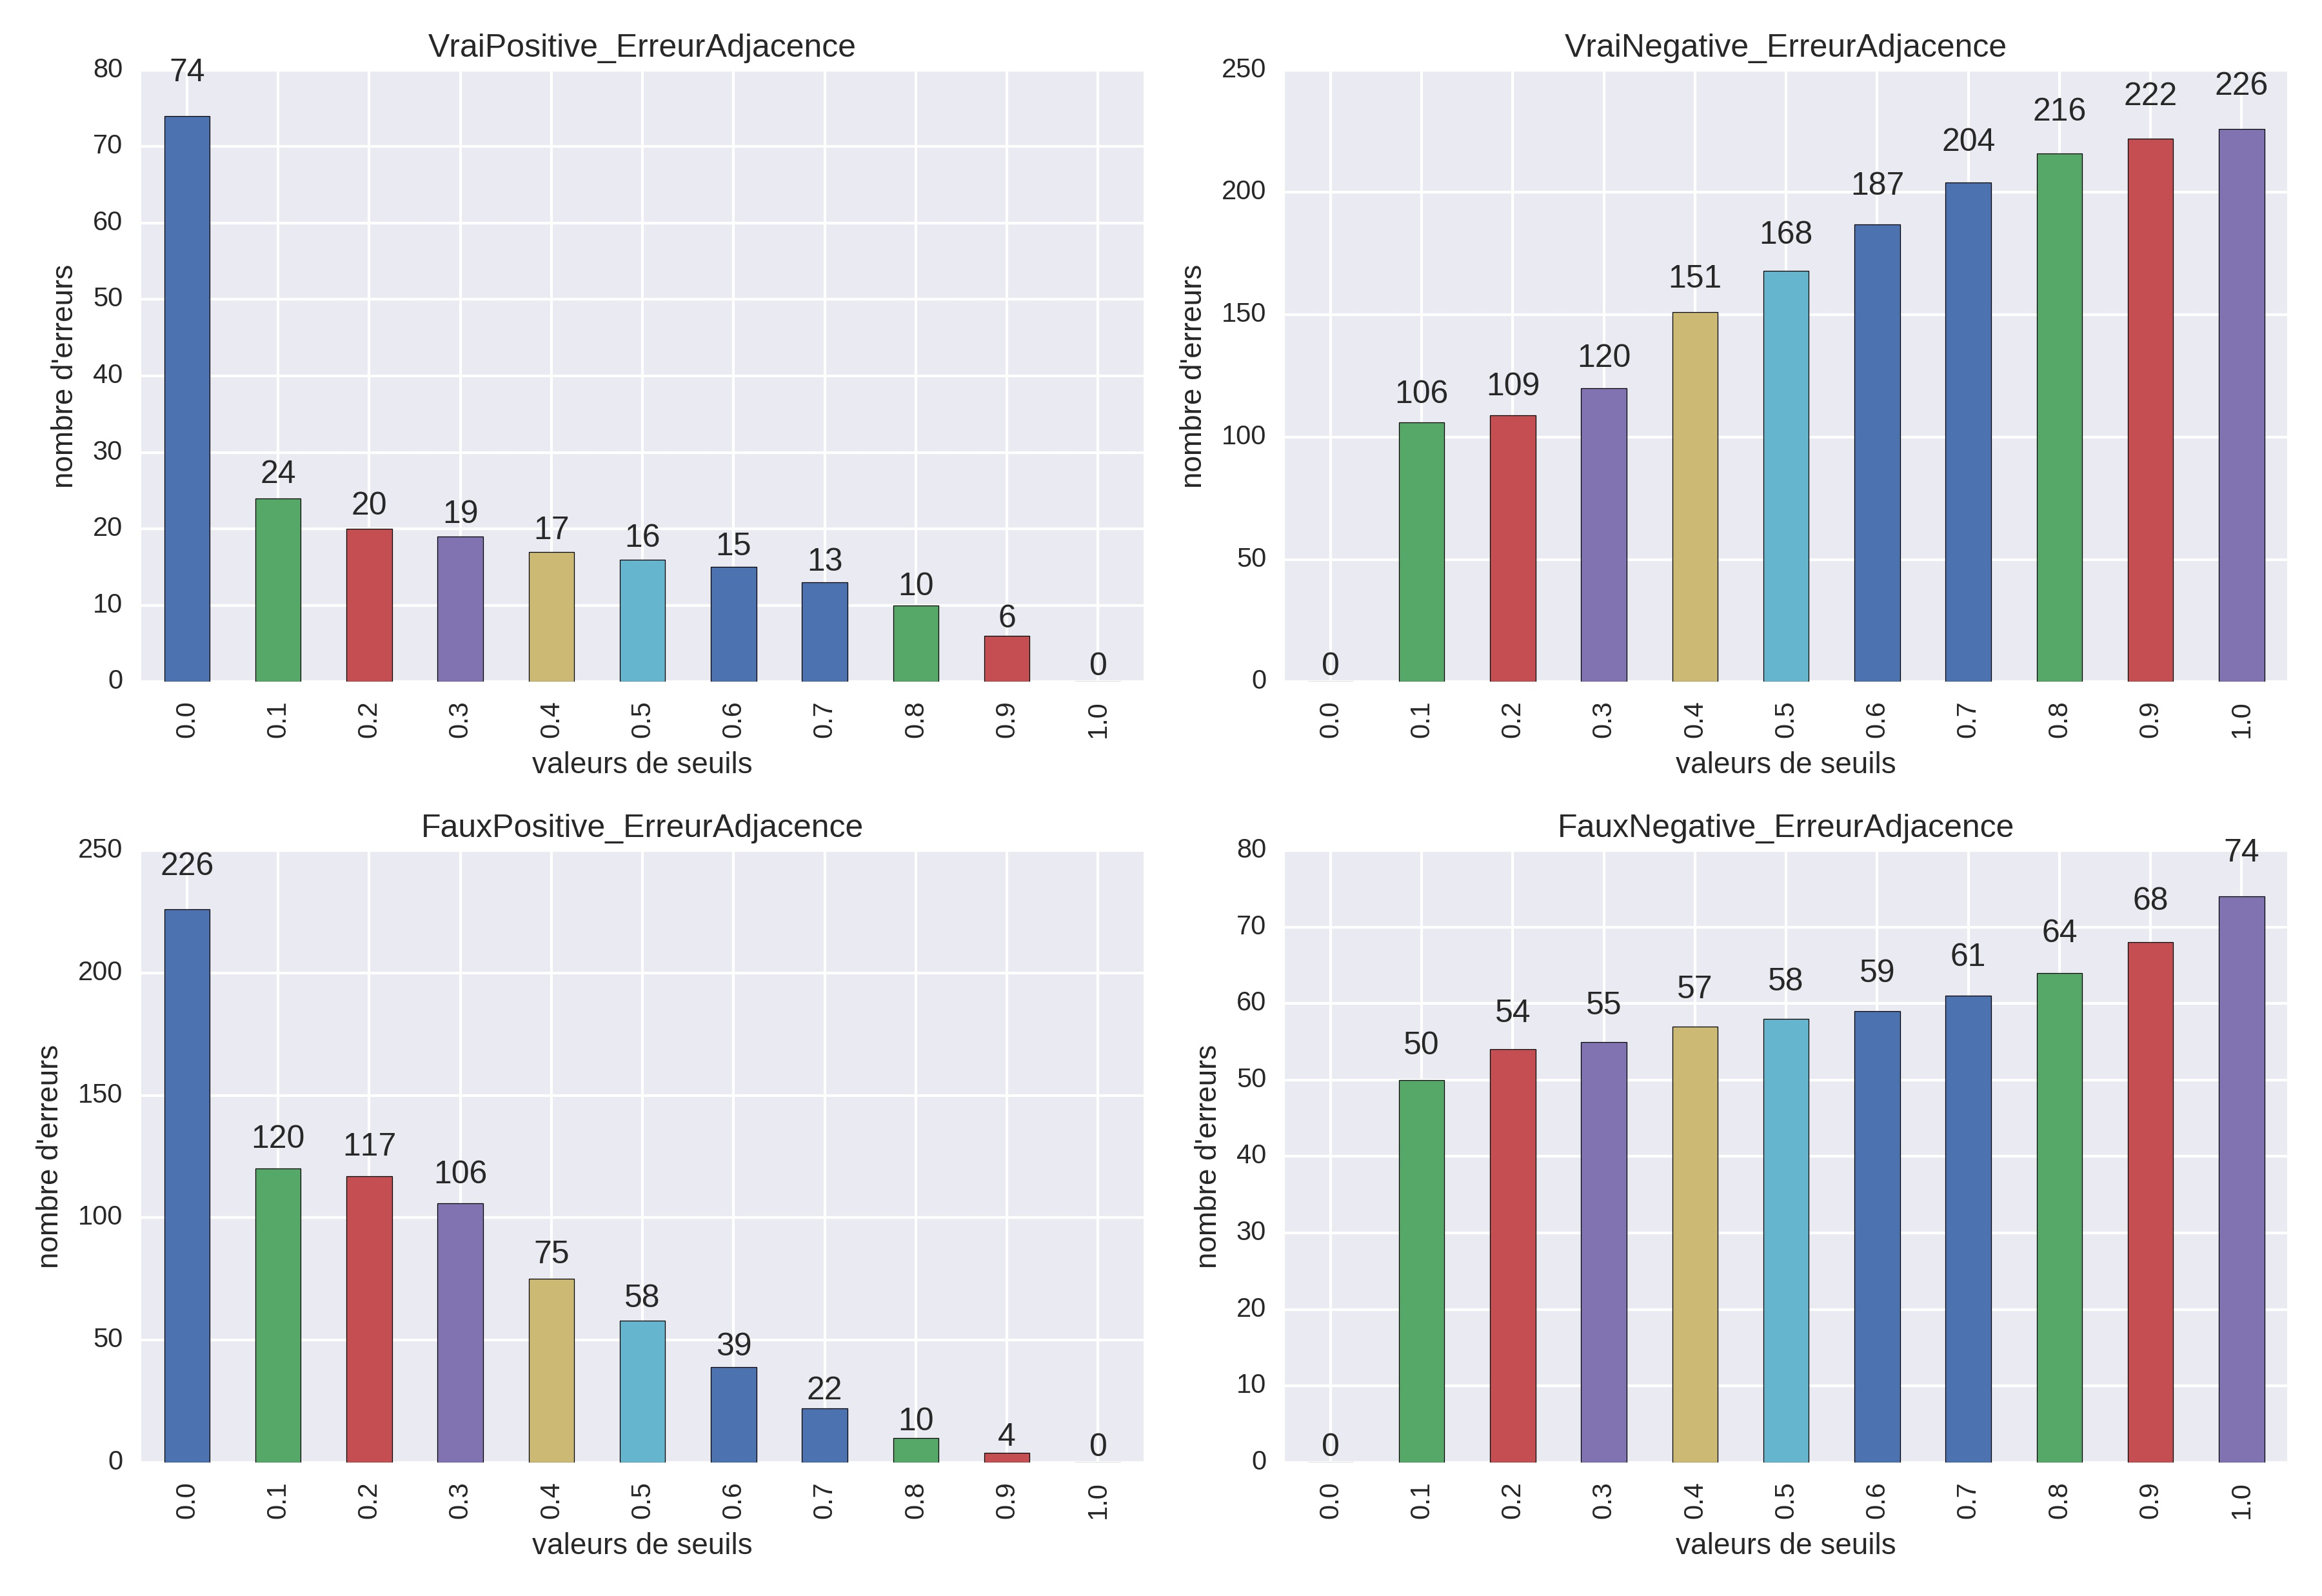
\includegraphics[width=500pt,height=250pt]{distrib_relationAdjacence_seuils.jpeg}
\caption{ Distribution des valeurs de corr\'elation sur un graphe g\'en\'er\'e de $30$ sommets et de degr\'e maximal de $5$.
.}
\label{distrib_relationAdjacence_seuils} 
\end{figure}
% \FloatBarrier
%---------------- distributionsCases01avecCoefficientAsymetries ------------------
Par exemple,  le graphe de corr\'elation $G_s$ contient 
$17$ cases {\em vrais positives}, 
$151$ cases {\em vrais n\'egatives}, 
$75$ cases {\em fausses positives} et 
$57$ cases {\em fausses n\'egatives} pour un seuil $s=0.4$.

	\subsection{Protocole d'exp\'erimentation des graphes  $G_s$ de corr\'elation} 
		% ------------- recapProtocoleEtudeSeuil -------------
\begin{figure}[htb!] 
\centering
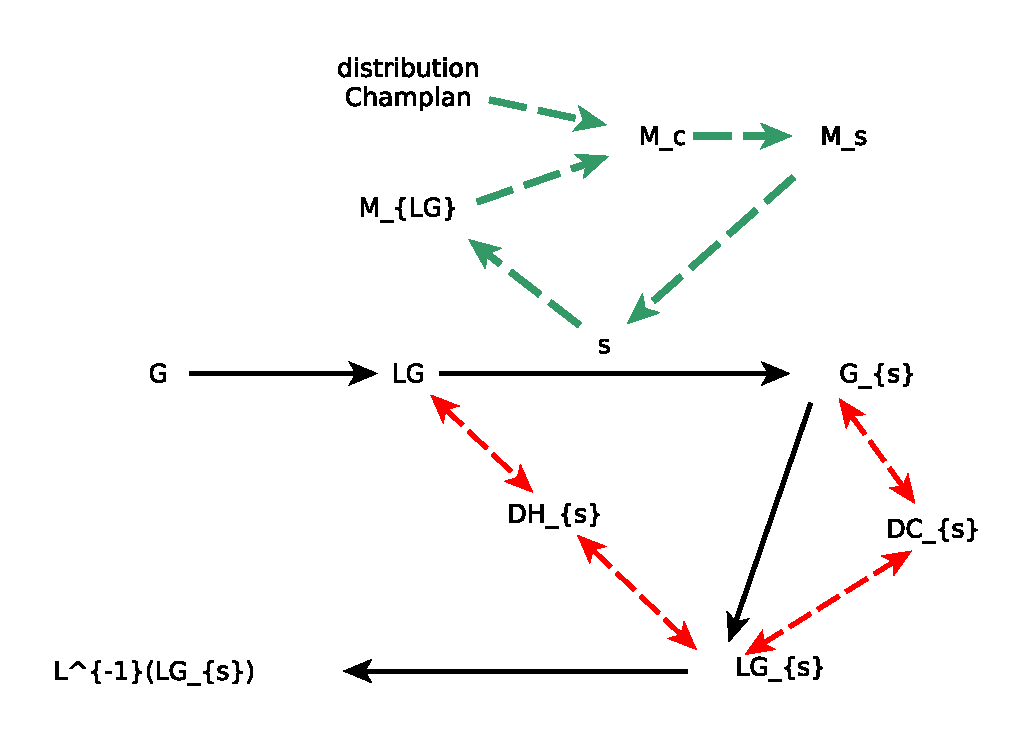
\includegraphics[scale=0.750]{recapProtocoleEtudeSeuil.eps}
\caption{\'Etapes de l'exp\'erimentation :  
1) on g\'en\`ere le graphe $G$ et son line-graphe $LG$, 
2) on  g\'en\`ere la matrice de corr\'elation $M_c$ du line-graphe $LG$   \`a partir de la distribution des valeurs de corr\'elation du graphe de Champlan puis on lui applique une valeur de seuil $s$ pour obtenir le graphe $G_{s}$, 
3) on applique les algorithmes de d\'ecouverte et de correction pour avoir un line-graphe $LG_{s}$. $LG_{s}$ et  $G_{s}$ diff\`erent de $DC_{s}$ ar\^etes. $LG_{s}$ a $DH_{s}$ cases modifi\'ees par rapport \`a $LG$, 
4) $L^{-1}(LG_{s})$ est le graphe racine de $LG_{s}$. 
}
\label{recapProtocoleEtudeSeuil} 
\end{figure}
% FloatBarrier
% ------------- recapProtocoleEtudeSeuil -------------

Le but de notre couple d'algorithmes est de corriger les cases erron\'ees dans $M_s$ afin que la matrice propos\'ee $M'_{s}$ soit la matrice d'adjacence d'un line-graphe $LG_s$ et que la distance de Hamming entre $LG_s$ et $LG$ soit minimale. 
Pour ce faire, nous recherchons la valeur du seuil $s$ qui mininise la distance de Hamming entre $LG_s$ et $LG$.
\newline

Nous g\'en\'erons les graphes dans les m\^emes conditions que l'exp\'erimentation $1$ de la section \ref{experimentation1} avec de petites modifications. D'abord, le nombre de graphes g\'en\'er\'es est de $150$. Ensuite, nous construisons une matrice de corr\'elation dont les \'etapes sont d\'ecrites dans la section \ref{affectationValeursProbabilites}. Et enfin, l'ajout des cases erron\'ees est r\'ealis\'e \`a partir d'un seuil $s$ dans la matrice de corr\'elation $M_c$ comme cela est expliqu\'e dans la section \ref{experimentation2GenerationMatriceProbabiliteAvecSeuil}. 
Les \'etapes de l'exp\'erimentation sont r\'esum\'ees dans la figure \ref{recapProtocoleEtudeSeuil}.

Nous consid\'erons que l'approche {\em al\'eatoire sans remise} (tableau \ref{tab:recapApprocheCorrection}) pendant l'algorithme de correction. Mais les fonctions de co\^uts des ar\^etes utilisent les valeurs de corr\'elation comme suit:
\begin{enumerate} [label = (\alph*)]
\item {\em Unitaire} : l'ajout et la suppression d'une ar\^ete ont un co\^ut de $1$.
\item {\em Normale} : l'ajout d'une ar\^ete \`a la case $M_s[i,j]$ a un co\^ut \'egal \`a sa valeur de corr\'elation $M_c[i,j]$ et la suppression d'une ar\^ete a un  co\^ut $1-M_c[i,j]$.
\item {\em Ajout} : l'ajout d'une ar\^ete \`a la case $M_s[i,j]$ a un co\^ut $M_c[i,j]$ alors que la suppression \`a cette case a un co\^ut $2 \times (1-M_c[i,j])$.
\item {\em Suppression} : la suppression d'une ar\^ete \`a la case $M_s[i,j]$ a un co\^ut $1-M_c[i,j]$ alors que l'ajout d'une ar\^ete \`a cette case a un co\^ut $2 \times M_c[i,j]$.
\end{enumerate}
Nous allons comparer les distances de Hamming et le pourcentage de cases corrig\'ees pour en d\'eduire la bonne valeur de seuil.



	\subsection{Analyses des r\'esultats}
	Nous allons d\'ecrire l'\'evolution du pourcentage des cases corrig\'ees en fonction de la valeur du seuil pour la fonction de co\^ut {\em normale}. Ensuite nous d\'eterminons l'influence de la valeur de seuil sur le nombre de cases corrig\'ees et enfin nous recherchons la meilleure fonction de co\^ut et l'influence des fonctions de co\^ut sur l'\'evolution des distances de Hamming.
		\subsubsection{\'Evolution du pourcentage de cases corrig\'ees}
			
Pour mesurer le pourcentage de cases corrig\'es, nous allons proc\'eder comme suit :
\begin{enumerate}[label = (\alph*)]
	\item Consid\'erer les cases {\em fausses positives} dans la matrice $M_s$ puis repr\'esenter le nombre de cases {\em fausses positives} pour chaque valeur de seuil. 
	Le graphique $(a)$ de la figure \ref{graphiquesFctCoutNormale} correspond \`a  la comparaison des seuils par rapport au nombre de cases {\em fausses positives} avant la correction.
	Nous remarquons qu'il n'y a aucune case {\em fausse positive} dans $M_s$ pour $s\in\{0.8,0.9\}$. Ce nombre croit quand le seuil $s$ decroit ($s \rightarrow 0$).
	
	\item Consid\'erer les cases {\em fausses n\'egatives} dans la matrice $M_s$ puis repr\'esenter le nombre de cases {\em fausses n\'egatives} pour chaque valeur de seuil.  Le graphique $(b)$ de la figure \ref{graphiquesFctCoutNormale}  correspond \`a la comparaison des seuils par rapport au nombre de cases {\em fausses n\'egatives} avant la correction. Le nombre des cases {\em fausses n\'egatives} est nul pour $s \not \in \{0.8,0.9\}$. 

	\item Consid\'erer les cases {\em fausses positives} apr\`es la correction de $G_s$ (matrice $M'_s$) puis repr\'esenter le nombre de cases {\em fausses positives} pour chaque valeur de seuil. Le graphique $(c)$ de la figure \ref{graphiquesFctCoutNormale} correspond \`a  la comparaison des seuils par rapport au nombre de cases {\em fausses positives} apr\`es la correction.
	 Le nombre de cases baisse quand $s \le 0.7$ puis augmente $s>0.7$.
	 
	\item Consid\'erer les cases {\em fausses n\'egatives} apr\`es la correction de $G_s$ (matrice $M'_s$) puis repr\'esenter le nombre de cases {\em fausses n\'egatives} pour chaque valeur de seuil. Le graphique $(d)$ de la figure \ref{graphiquesFctCoutNormale} correspond \`a la comparaison des seuils par rapport au nombre de cases {\em fausses n\'egatives} apr\`es la correction. Le nombre de cases varie peu quand $s < 0.4$ puis baisse quand $s = \{0.5, 0.6\}$ avant d'atteindre sa valeur minimum \`a $s = 0.7$. Il augmente $s>0.7$.
	
	\item Repr\'esenter les distances de Hamming moyennes de chaque graphe pour chaque seuil. Le graphique $(e)$ de la figure \ref{graphiquesFctCoutNormale} correspond \`a la comparaison des seuils en fonction de la distance de Hamming de chaque seuil.
	La distance de Hamming baisse quand $s \rightarrow 0.7$ avec sa valeur minimum \`a $s = 0.7$ puis augmente quand $s > 0.7$. 
\end{enumerate}
Rappelons que les diff\'erents graphiques sont rang\'es par ordre croissant et 
les distances de Hamming sont obtenues \`a partir la fonction de co\^ut {\em normale}.

Nous distinguons trois familles de seuils:
\begin{itemize}
	\item Les seuils $s < 0.7$ qui baissent le nombre de cases  {\em fausses positives} et augmentent celui des cases {\em fausses n\'egatives} apr\`es l'algorithme de correction. 
	Ils n'ont pas d'effets r\'eels sur la distance de Hamming car il y a un transfert d'\'el\'ements de l'ensemble des cases   {\em fausses positives} \`a celui des {\em fausses n\'egatives} et vice-versa. 
	\`A cet effet, on remarque  qu'il y a $20\%$ de cases {\em fausses n\'egatives} apr\`es la correction alors qu'il n'en existait aucune case {\em fausse n\'egative} avant la correction. 
	Il en est de m\^eme avec les cases  {\em fausses positives}  dont le nombre diminue de $20\%$  \'egalement pendant la correction. Ces seuils n'ont aucune influence sur les cases erron\'ees.
	% -------- graphiquesFctCoutNormale ---------
\begin{figure}[htb!] 
\centering
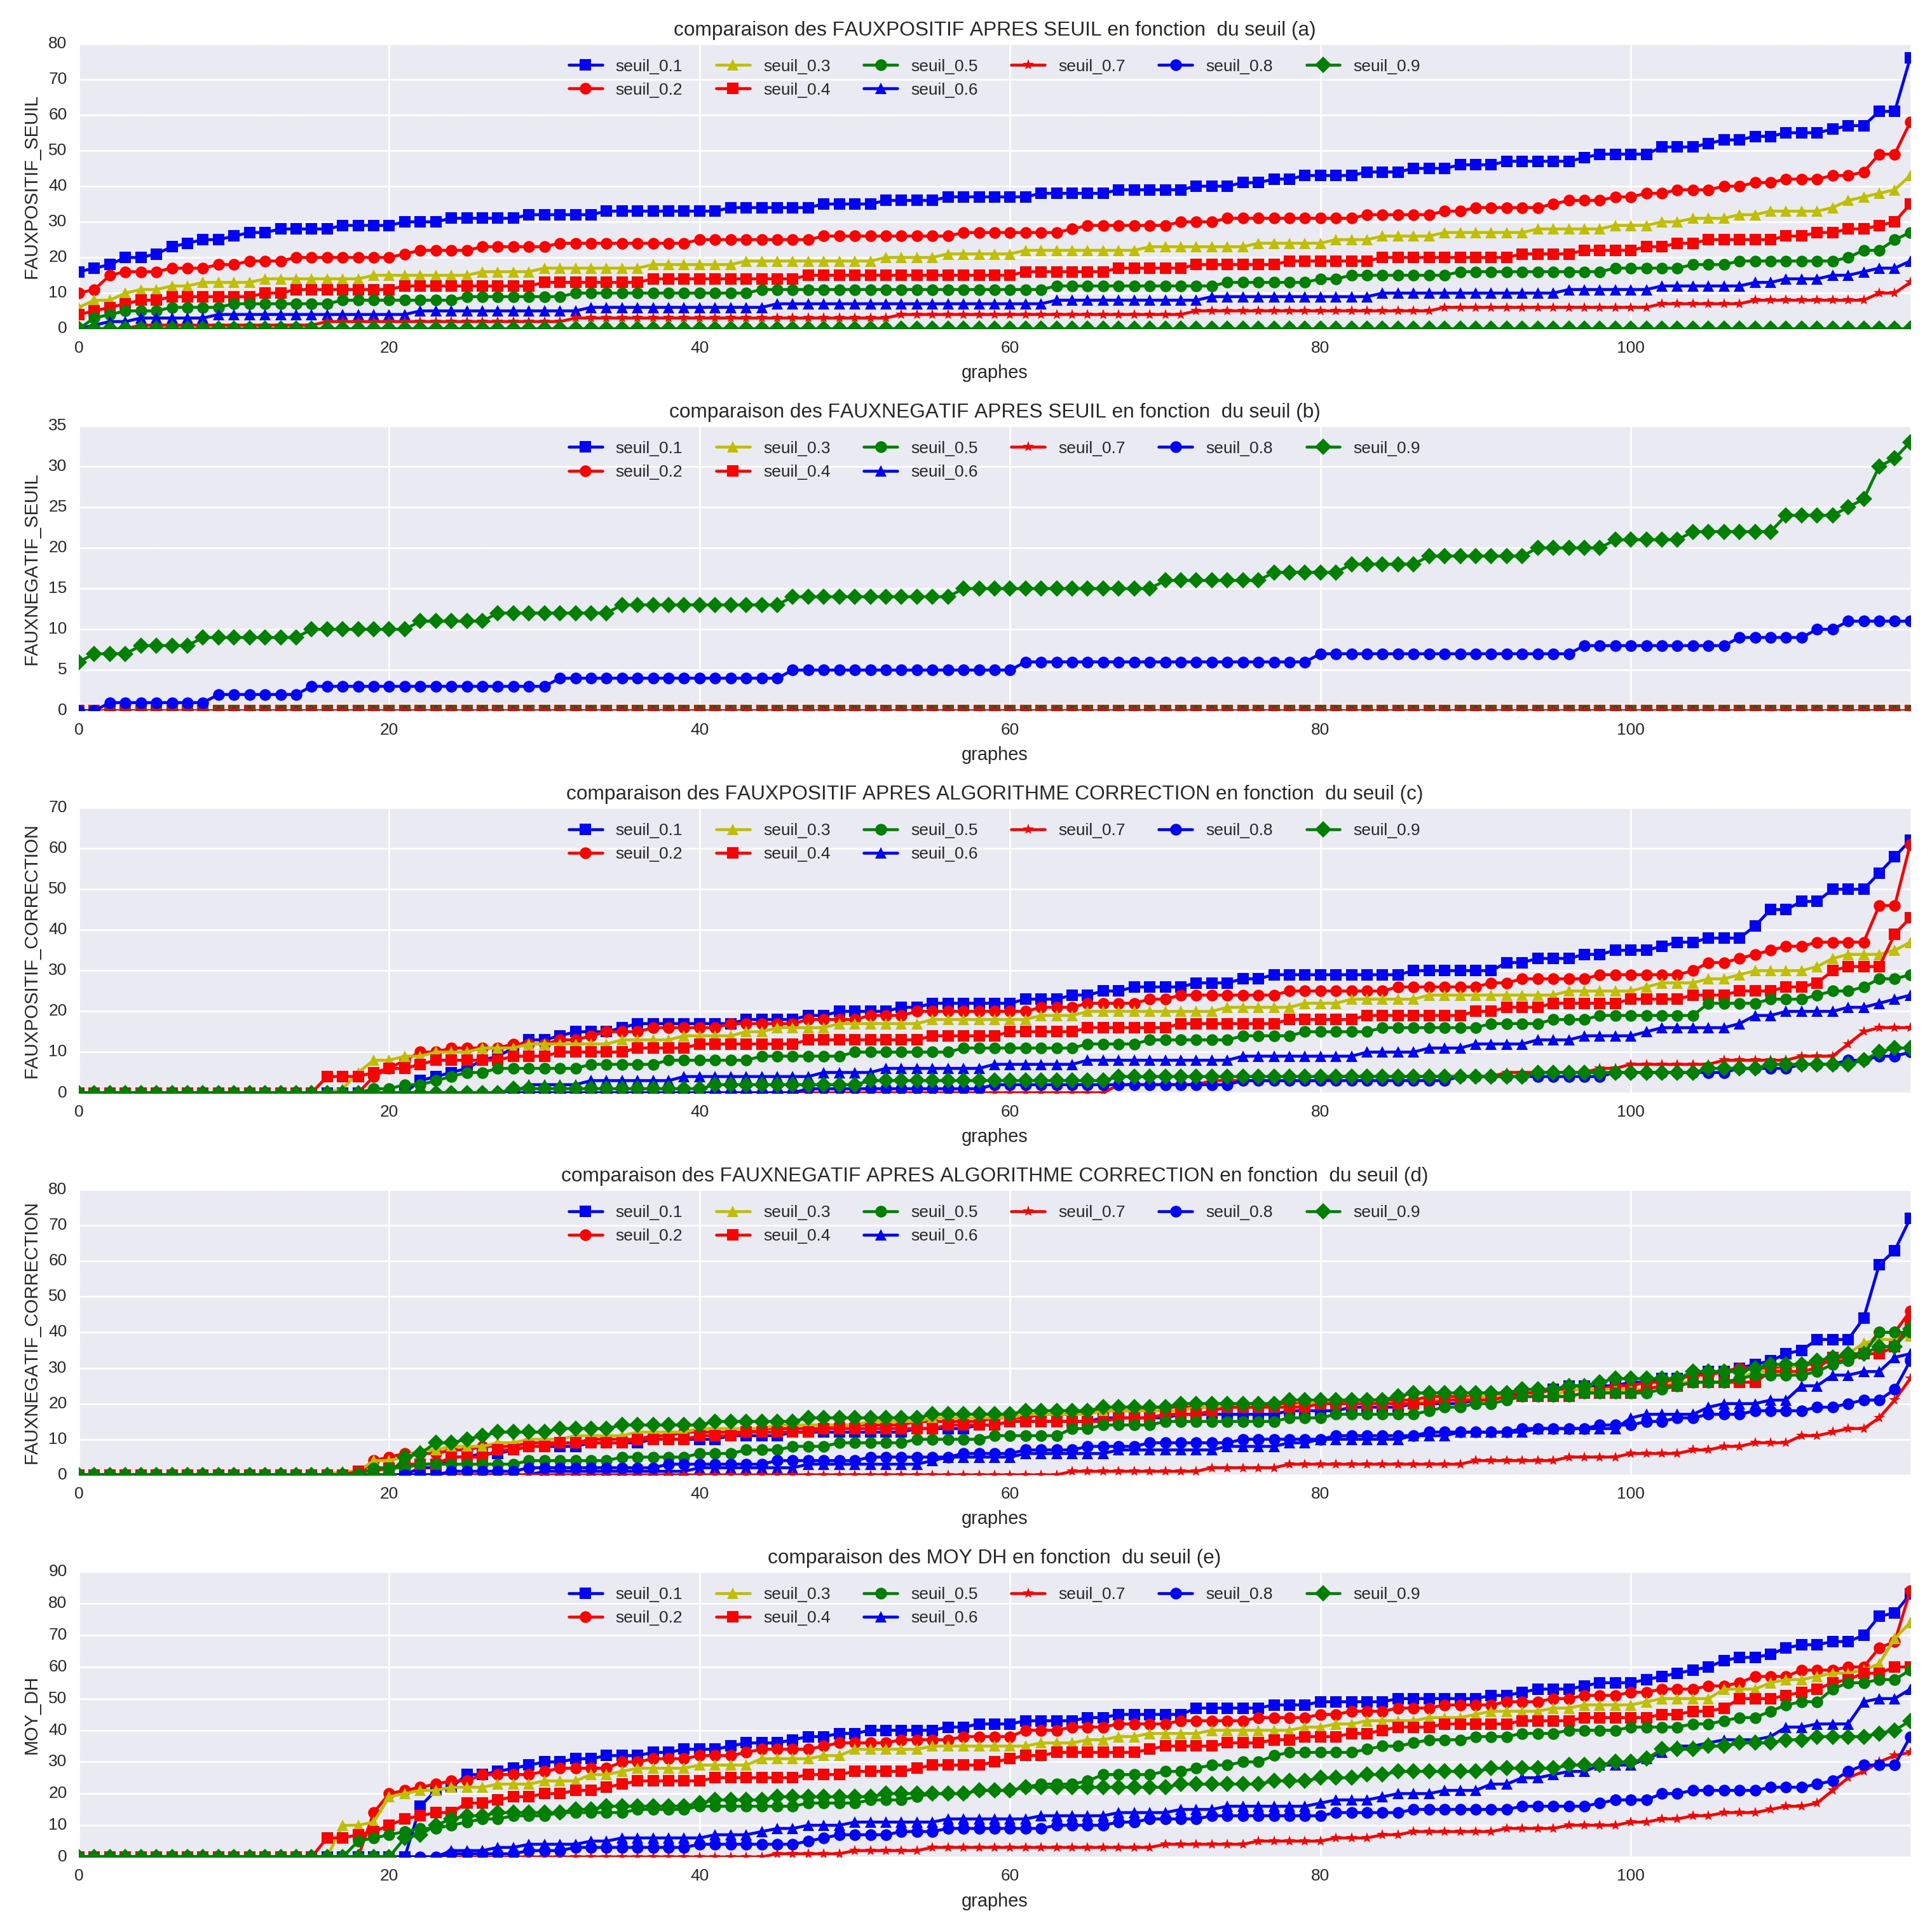
\includegraphics[scale=0.18]{choix_du_seuil_pour_fauxPositif_seuil_fauxNegatif_seuil_fauxPositif_correction_fauxNegatif_correction_moy_dh_aleatoire_normale.jpeg}
\caption{ Choix du seuil : (a) cases {\em fausses positives} dans la matrice $M_s$; (b) cases {\em fausses n\'egatives} dans la matrice $M_s$,(c) cases {\em fausses positives} dans la matrice $M'_s$; (d) cases {\em fausses n\'egatives} dans la matrice $M'_s$; (e) comparaison des seuils selon $moy\_DH$ }.
\label{graphiquesFctCoutNormale} 
\end{figure}
\FloatBarrier
% -------- graphiquesFctCoutNormale ---------

	\item Les seuils $s > 0.7$ qui augmentent le nombre de cases {\em fausses positives} et baissent celui des cases {\em fausses n\'egatives} apr\`es l'algorithme de correction. En effet, 
	le nombre de cases {\em fausses positives} est nul dans $M_s$ parce qu'il n'y a aucune case \`a $1$ ayant une valeur inf\'erieure \`a $s$ dans la distribution.
	Dans $M'_s$, le nombre moyen de cases {\em fausses positives} est de $1.76$ pour $s=0.8$ et de $2.33$ pour $s=0.9$. 
	Il y a l'ajout d'ar\^etes dans le graphe $LG_s$ parce que le nombre d'ar\^etes \`a supprimer pour corriger un sommet est tr\`es \'elev\'e et cela implique que le co\^ut de la correction par la suppression d'ar\^etes est tr\`es on\'ereux par rapport \`a celui de l'ajout d'ar\^etes. 
	Ainsi \`a chaque sommet \`a corriger, l'algorithme ajoute plus d'ar\^etes qu'il en supprime et certaines ar\^etes ajout\'ees appartiennent \`a l'ensemble des ar\^etes de $LG$.
	 Cela fait baisser les cases {\em fausses n\'egatives} comme nous le constatons avec les chiffres suivants : le nombre moyen de ces cases passe de  $6.7$ \`a $2.5$  pour $s = 0.8$ et de $17.7$ \`a $12.5$ pour $s = 0.9$.
	
	\item Le seuil $s=0.7$ qui diminue le nombre de cases {\em fausses n\'egatives} et {\em fausses positives}. En effet, le nombre moyen de cases erron\'ees est faible $< 10$ avant la phase de correction et il est $ \le 5$ apr\`es la correction. 
	Nous remarquons aussi les cases erron\'ees sont majoritairement des cases {\em fausses n\'egatives} apr\`es la correction.
	La pr\'esence de ces cases provient du co\^ut de modification des ar\^etes car la compression $\pi_1,\pi_2, \pi_s$ de co\^ut minimale n\'ecessite la suppression d'ar\^etes existantes.
	En effet, la matrice $M_s$ ne contient que des cases {\em fausses positives}. Pour trouver des bipartitions coh\'erentes (voir d\'efintion \ref{cliquesCoherentes}) autour des sommets \`a corriger, il faut ajouter beaucoup d'ar\^etes pour chaque partition et cela fait croitre le co\^ut de la correction. 
	Nous avons remarqu\'e aussi que la suppression de quelques ar\^etes permet d'obtenir des cliques qui correspondent \`a des sommets de $G$. L'algorithme pr\'ef\`ere alors supprimer des ar\^etes car elles sont peu par rapport aux ar\^etes \`a ajouter et aussi le co\^ut de la suppression d'ar\^etes est faible.
	 La distance de Hamming obtenue avec ce seuil est minimale par rapport aux autres seuils. Ce seuil fournit alors une meilleure correction des sommets de ${\cal C}$. 
	
\end{itemize}

{\bf Conclusion} : 
nous pouvons conclure que la repartition des cases erron\'ees avant la phase de correction a une influence sur l'algorithme de correction. 
Ainsi, le choix du seuil dans le bon intervalle permet de r\'eduire le nombre de cases erron\'ees et fournit une excellente correction des sommets de ${\cal C}$. 
Cependant,  les seuils diff\'erents du bon seuil  entraine que la fonction de co\^ut n'a aucune influence sur les corrections parce que l'algorithme corrige peu de cases erron\'ees mais ajoute aussi des cases {\em fausses positives} et {\em fausses n\'egatives} dans la m\^eme proportion. 

% ----------- comparaisonFctCoutUnitaireNormale -----------------
\begin{figure}[htb!] 
\centering
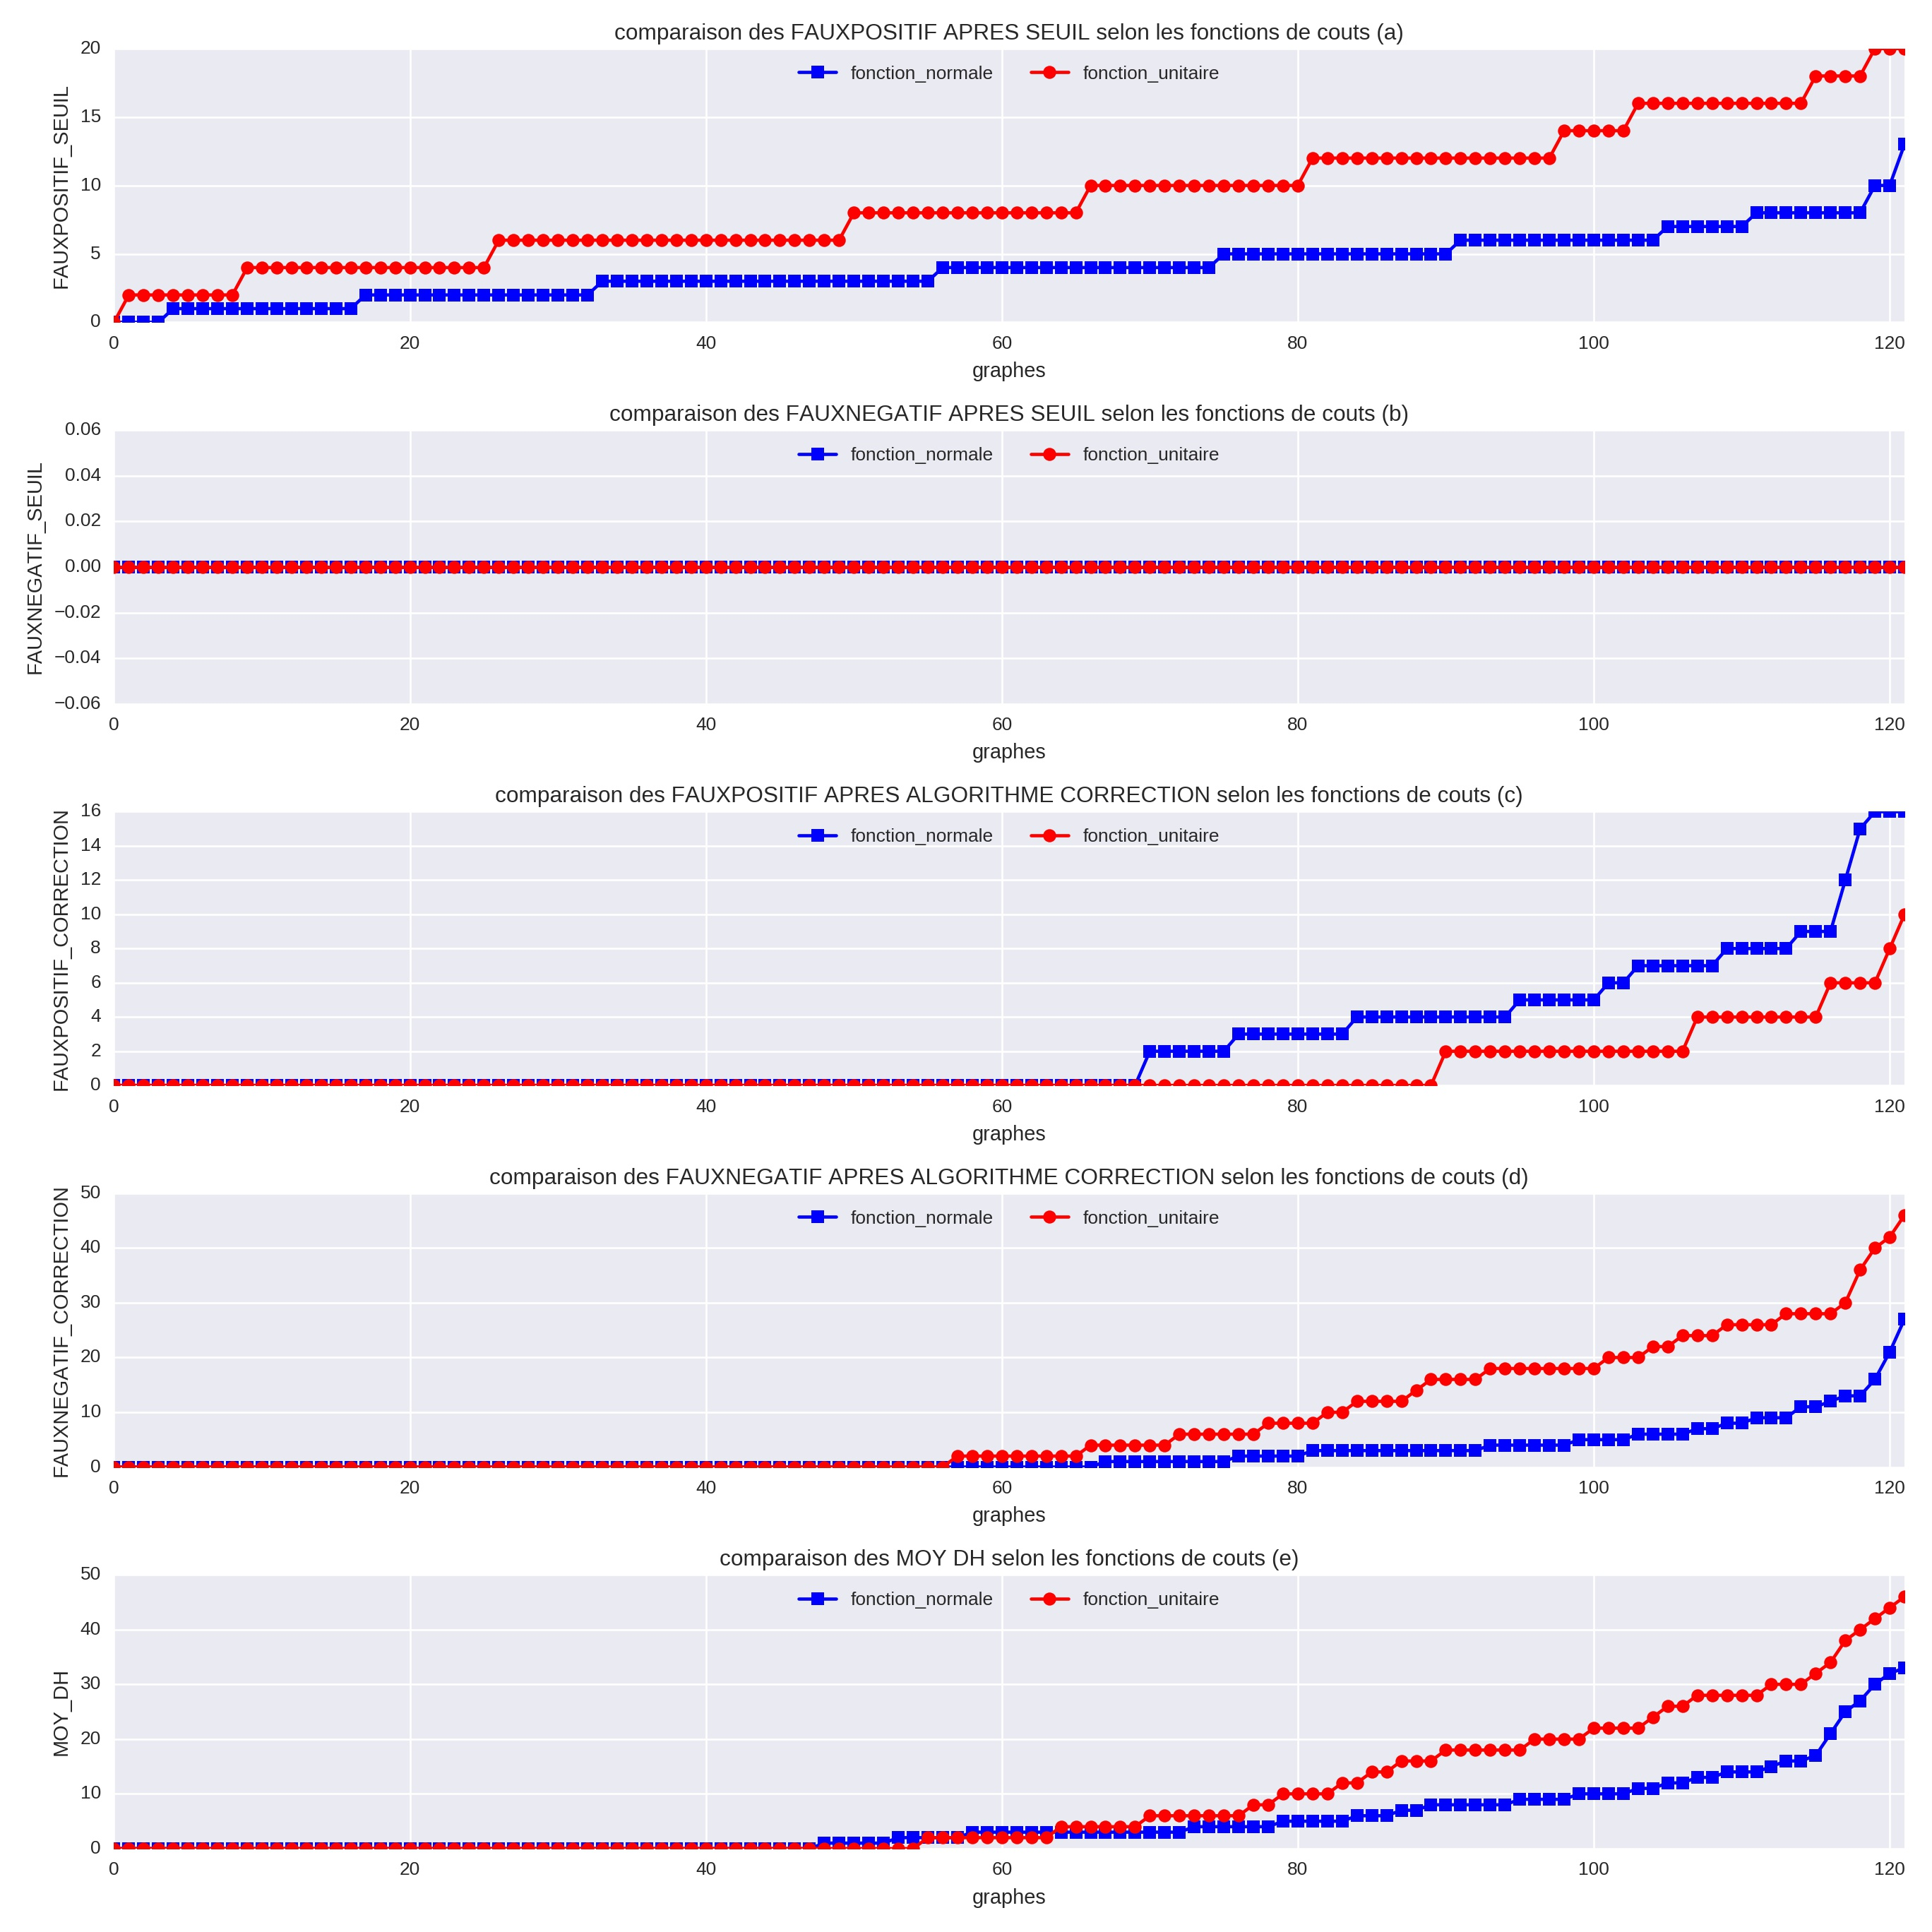
\includegraphics[scale=0.20]{choix_fct_cout_pour_fauxPositif_seuil_fauxNegatif_seuil_fauxPositif_correction_fauxNegatif_correction_moy_dh_aleatoire_s_07.jpeg}
\caption{ Comparaison entre les fonctions de co\^ut {\em unitaire} et {\em normale}: (a) cases {\em fausses positives} dans la matrice $M_s$; (b) cases {\em fausses n\'egatives} dans la matrice $M_s$; (c) cases {\em fausses positives} dans la matrice $M'_s$; (d) cases {\em fausses n\'egatives} dans la matrice $M'_s$; (e) comparaison des fonctions de co\^ut selon $moy\_DH$.}
\label{comparaisonFctCoutUnitaireNormale} 
\end{figure}
 \FloatBarrier
% ----------- comparaisonFctCoutUnitaireNormale -----------------


		\subsubsection{Influence de la valeur du seuil }
			%choix du seuil
Les seuils inf\'erieurs \`a $0.7$ correspondent \`a une reduction des cases {\em fausses positives} et une augmentation de cases {\em fausses n\'egatives} dans la matrice de correction. Dans ce cas, nous constatons que le nombre des  cases
{\em fausses positives} baisse \'enormement quand $s \rightarrow 0.7$. Ce ph\'enom\`ene s'explique par le co\^ut de modifications des ar\^etes (normale) et le nombre faible de cases erron\'ees au voisinage de  $0.7$. L'augmentation des cases  {\em fausses n\'egatives} provient du  fonctionnement de notre algorithme de correction.  L'algorithme doit ajouter des ar\^etes dans une partition $\pi_1 ~ou~ \pi_2$ au voisinage d'un sommet pour en faire une clique. Le nombre \'elev\'e de cases  {\em fausses n\'egatives} n\'ecessite l'ajout de beaucoup d'ar\^etes.
\newline
Les seuils sup\'erieurs \`a $0.7$ correspondent \`a l'augmentation des  cases {\em fausses positives} et la baisse de celles {\em fausses n\'egatives}. 
La pr\'esence de cases {\em fausses positives} en grand nombre entraine l'algorithme de correction dans deux cas :
l'ajout de peu d'ar\^etes  et 
la suppression de beaucoup d'ar\^etes pour atteindre un line-graphe.
Dans le premier cas, la distance de Hamming est faible mais le line-graphe est diff\'erent du line-graphe de $G_s$. 
Dans ce second cas, la distance de Hamming est tr\`es \'elev\'ee et nous avons tr\`es peu de chance de retrouver le line-graphe de $G_s$.
\newline

{\bf Conclusion} : 
le meilleur compromis de seuil est celui qui baisse les cases {\em fausses positives}  et les cases {\em fausses n\'egatives} apr\`es l'algorithme de correction.  Le seuil capable d'atteindre ce r\'esultat est dans l'intervalle $s=]0.6,0.7]$. Dans la suite du chapitre, nous retenons $s=0.7$.
Avec ce seuil, les distances de Hamming sont aussi les plus faibles (graphique $(e)$ figure \ref{graphiquesFctCoutNormale}). 
		\subsubsection{Choix de la fonction de co\^ut et impact sur les distances de Hamming }
			
Nous rappelons que la fonction de co\^ut est d\'efinie par la somme des co\^uts des cases \`a modifier pour corriger chaque sommet de $\cal C$ pendant l'algorithme de correction. 
Le co\^ut de correction d'un sommet est le co\^ut minimal de toutes les cases modifi\'ees. 
Nous recherchons alors la fonction de co\^ut qui minimise globalement le co\^ut de correction des sommets de $\cal C$.
%Pour ce faire, nous comparons les fonctions de co\^ut {\em unitaire}, {\em normale}, {\em ajout} et {\em suppression}. 
Pour ce faire, nous comparons d'abord les fonctions de co\^ut {\em unitaire} et {\em normale} parce que nous souhaitons savoir s'il est pr\'ef\'erable d'utiliser les valeurs de corr\'elations dans les co\^uts des op\'erations. Puis nous comparons la meilleure des deux fonctions avec celles {\em ajout} et {\em suppression}.
%Nous repr\'esentons les distances $moy\_DH$ des diff\'erentes fonctions de co\^ut  sur la figure \ref{comparaisonFctCoutUnitaireNormale}. 
La figure \ref{comparaisonFctCoutUnitaireNormale} contient 
\begin{itemize}
	\item La comparaison des distances de Hamming entre les  fonctions de co\^ut {\em unitaire} et {\em normale} (graphique $(e)$).
	\item La comparaison du nombre de cases {\em fausses n\'egatives} entre les $2$ fonctions de co\^ut avant l'algorithme de correction (graphique $(b)$).
	\item  La comparaison du nombre de cases {\em fausses n\'egatives} entre les $2$ fonctions de co\^ut apr\`es l'algorithme de correction (graphique $(d)$).
	\item La comparaison du nombre de cases {\em fausses positives} entre les $2$ fonctions de co\^ut avant l'algorithme de correction (graphique $(a)$).
	\item  La comparaison du nombre de cases {\em fausses positives} entre les $2$ fonctions de co\^ut apr\`es l'algorithme de correction (graphique $(a)$).
\end{itemize}
Les distances de Hamming et les nombres de cases sont ordonn\'ees par ordre croissant.
%\newline
% ----------- comparaisonFctCoutNormaleAjoutSuppression -----------------
\vspace{-0.5cm}
\begin{figure}[htb!] 
\centering
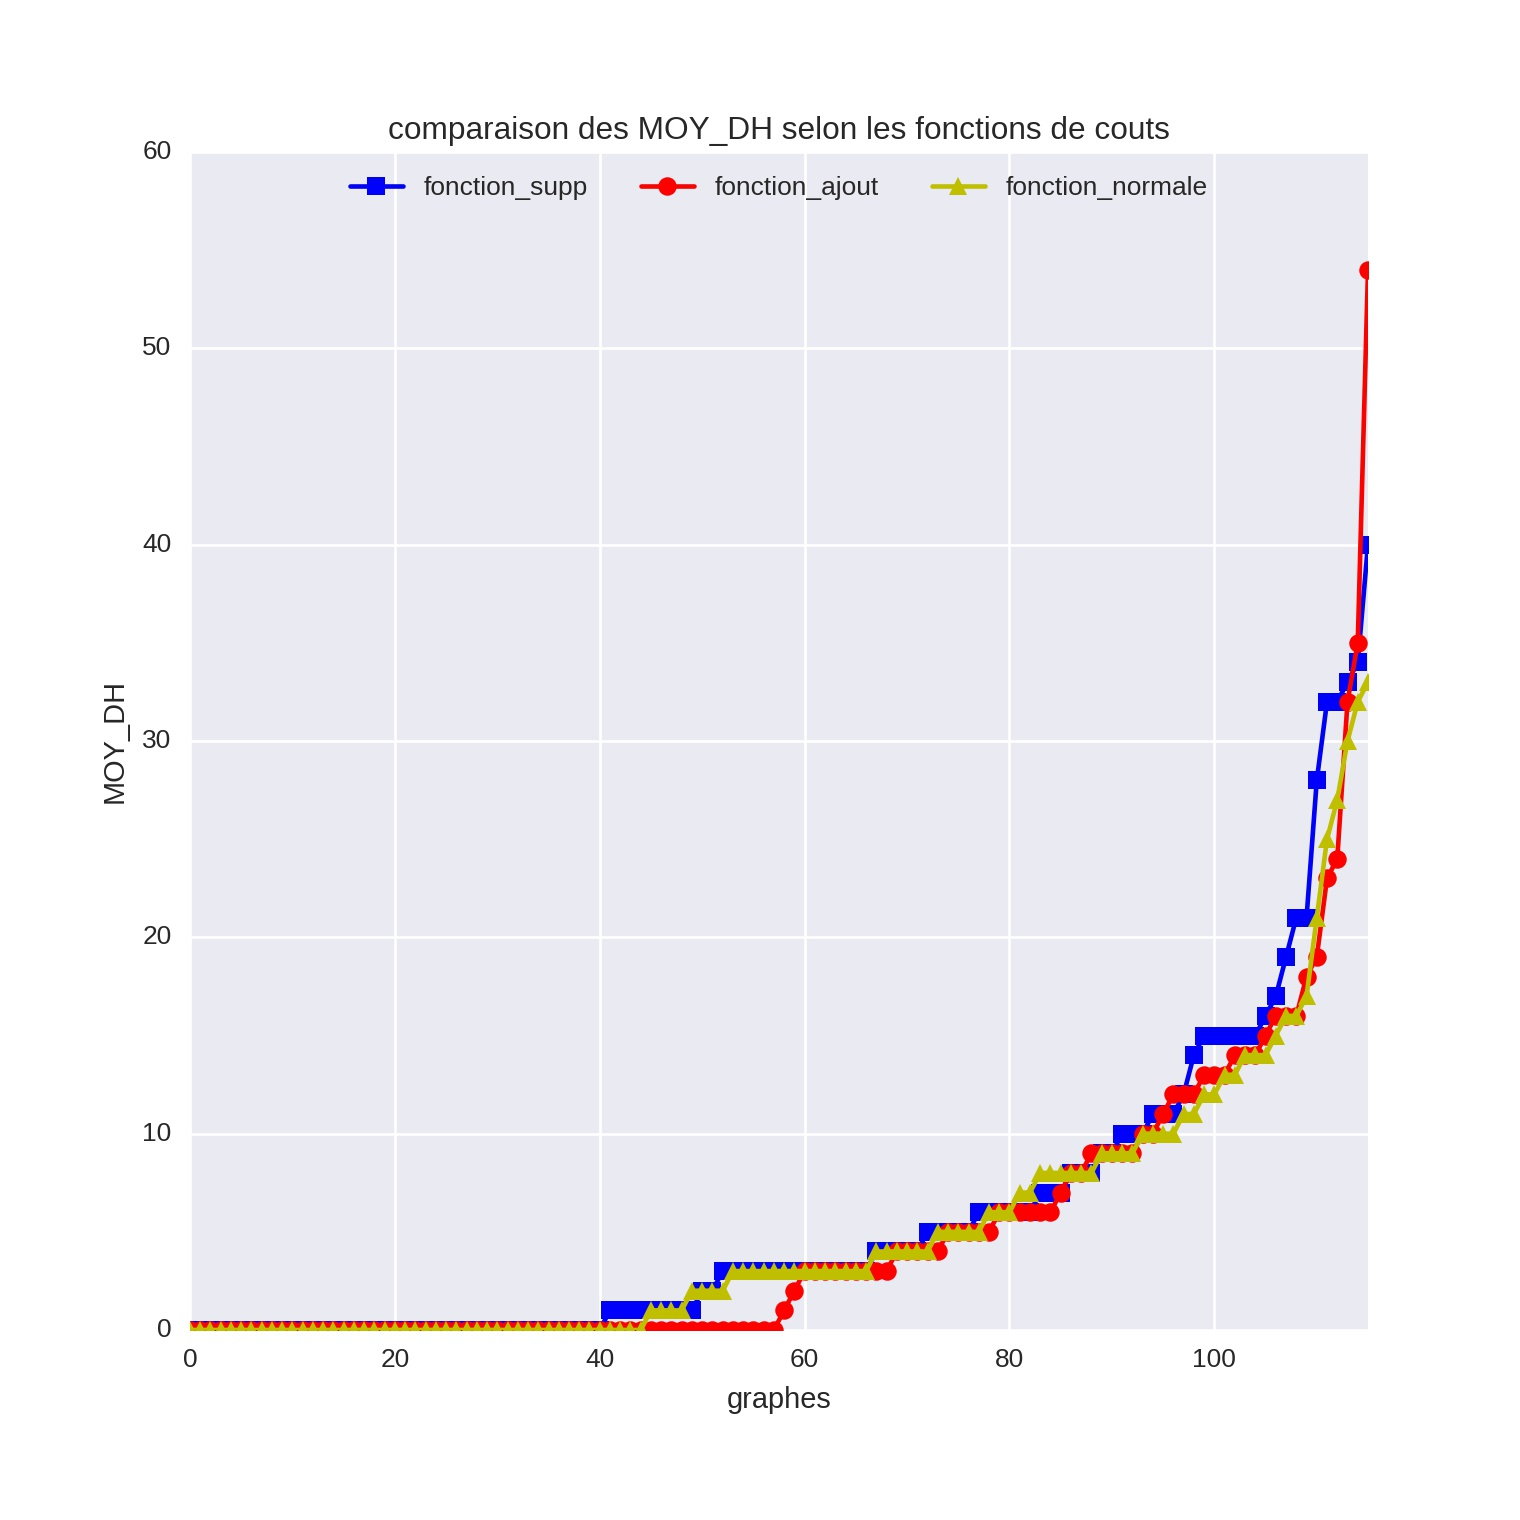
\includegraphics[scale=0.25]{comparaison_fct_couts_moy_dh_s_07_aleatoire_supp_ajout_normale.jpeg}
\caption{ Comparaison entre les fonctions de co\^ut {\em normale},  {\em ajout} et  {\em suppression} : la fonction {\em ajout} est la courbe en rouge, la fonction {\em normale} est en jaune et la fonction {\em suppression est en bleu}}
\label{comparaisonFctCoutNormaleAjoutSuppression} 
\end{figure}
 \FloatBarrier
% ----------- comparaisonFctCoutNormaleAjoutSuppression -----------------
Nous constatons que la courbe de la fonction {\em unitaire} est au dessus de celle de la fonction {\em normale} dans le graphique $(e)$ de la figure \ref{comparaisonFctCoutUnitaireNormale}.
Avec $s=0.7$, l'ensemble de cases \'erron\'ees sont des cases {\em fausses positives} (graphique $(c)$ de la figure \ref{comparaisonFctCoutUnitaireNormale}).
En appliquant les fonctions {\em unitaire} et {\em normale}, nous avons l'introduction de cases {\em fausses n\'egatives} et le nombre de ces cases est plus important dans la fonction {\em unitaire}. Ce nombre fait cro\^itre la distance de Hamming $moy\_DH$ parce que la correction a r\'eduit le nombre de cases {\em fausses positives} dans la fonction {\em normale} (voir les graphiques $(a)$ et $(c)$ de la figure  \ref{comparaisonFctCoutUnitaireNormale}).
Ce qui explique les faibles distances $moy\_DH$ de la fonction {\em normale}. La fonction {\em normale} donne de meilleurs r\'esultats et nous la choisissons dans le calcul des co\^uts de correction.
\newline

Par ailleurs, dans la figure \ref{comparaisonFctCoutNormaleAjoutSuppression}, les courbes des  fonctions  {\em normale}, {\em ajout} et {\em suppression} sont entremel\'ees et il ne se d\'egage aucun \'ecart significatif entre elles. Il est donc difficile de juger de l'influence d'une des fonctions sur la correction des sommets de $\cal C$.  
\newline 

{\bf Conclusion} :
 prioriser l'ajout \`a la suppression et vice versa n'a aucune influence sur les distances de Hamming quand nous utilisons les valeurs de corr\'elations. Toutefois,  il est pr\'ef\'erable de consid\'erer les corr\'elations dans le calcul du co\^ut de la modification d'une case parce que cela am\'eliore les distances $moy\_DH$ comme il est indiqu\'e dans le graphique $(e)$  de la figure \ref{comparaisonFctCoutUnitaireNormale}.
	\subsection{Conclusion de l'exp\'erimentation 2}	
		Nous avons g\'en\'er\'e des valeurs de corr\'elations pour toutes les cases de la matrice $M_{LG}$ en consid\'erant la distribution des valeurs de corr\'elation du r\'eseau \'electrique du data center {\em Champlan}. 
Les valeurs de corr\'elation suivent des lois normales asym\'etriques de param\`etre $\alpha = 5$ pour les cases \`a $0$ et  de param\`etre $\alpha = -5$ pour les cases \`a $1$.
La matrice de corr\'elation $M_c$ est construite \`a partir de ces corr\'elations.
Un ensemble $s \in S$ de seuils est appliqu\'e \`a la matrice $M_c$ pour la transformer en la matrice d'adjacence $M_s$ du graphe $G_s$. 
La matrice $M_s$ contient des cases {\em fausses n\'egatives} et {\em fausses positives}. 
Nous cherchons \`a minimiser la distance de Hamming en corrigeant le maximum de cases erron\'ees pendant l'algorithme de correction. Cela passe par la s\'election ad\'equate du seuil et de la fonction de co\^ut.
Apr\`es l'ex\'ecution de notre couple d'algorithmes, nous  avons d\'eduit que le bon seuil est contenu dans l'intervalle $s = ]0.6,0.7]$ et que la fonction {\em normale} est la meilleure fonction de co\^ut. 
L'utilisation du seuil $s$ et de la fonction {\em normale} ne garantissent pas la suppression totale des cases erron\'ees.  Mais elles minimisent leur nombre de telle sorte qu'un expert du m\'etier puisse effectuer les corrections manuellement qui conduisent au line-graphe $LG$ recherch\'e.
Dans la section suivante, nous nous int\'eressons aux graphes dans lesquels tous les sommets ne peuvent \^etre couverts par $1$ ou $2$ cliques. Ces graphes sont dits {\em grilles boucl\'ees}. 		

%---------------------------------------------------------------------------
%------- experimentation 3  graphes grilles boucl\'ees
%---------------------------------------------------------------------------	
\section{Exp\'erimentation 3 : algorithmes sur les grilles boucl\'ees}
	Nous consid\'erons des graphes dans lequels le voisinage d'un sommet peut \^etre couvert par  une ou deux cliques. L'ex\'ecution de l'algorithme de couverture sur chacun de ces graphes fournit une couverture vide. Cette famille de graphes est d\'esign\'ee graphes {\em grilles boucl\'ees}. Apr\`es l'ex\'ecution de l'algorithme de couverture, tous les sommets de la {\em grille boucl\'ee} sont dans l'ensemble $\cal C$ des sommets \`a corriger.
\newline
Dans cette section, nous \'evaluons les performances de nos algorithmes, particuli\`erement l'algorithme de correction en effectuant  des op\'erations de {\em suppression } et d'{\em ajout} d'ar\^etes uniquement.
Nous d\'eterminons une borne sup\'erieure de la distance line de ces graphes.
Nous comparons cette borne avec les r\'esultats obtenus par l'algorithme de correction avec l'approche {\em al\'eatoire sans remise} (voir tableau \ref{tab:recapApprocheCorrection}).
\newline
 Nous d\'ebutons notre analyse par la d\'efinition et la construction d'une grille boucl\'ee. Ensuite, nous d\'ecrivons le protocole d'exp\'erimentation sur des grilles boucl\'ees d'ordres diff\'erents. Enfin nous interpr\'etons les r\'esultats obtenus pour chaque op\'eration.
	\subsection{D\'efinition des grilles boucl\'ees et les distances line th\'eoriques}
%		Soient $k$ et $k'$ deux entiers pairs non nuls avec 
$k$ le nombre de sommets par colonnes et 
$k'$ le nombre de sommets par lignes et
$G_{k,k'}$ une grille boucl\'ee.

%Soit $G_{k,k'}$ une grille boucl\'ee de $$ laquelle $k$ et $k'$ d\'esignent le nombre de sommets  respectivement par lignes et colonnes. 
%Nous pr\'ecisons que les nombres $k$ et $k'$ sont {\em pairs}.




%Soit $G_{k,k'}$ la famille de graphes cellules dans laquelle $k$ et $k'$ d\'esignent le nombre de graphes cellules respectivement par lignes et colonnes.
%Nous pr\'ecisons que les nombres $k$ et $k'$ sont {\em impairs}.
%
%\begin{definition}
%Une cellule est un graphe biparti $K_{2,2}$ non orient\'e avec un cycle.
%\end{definition}
%
%\begin{definition}
%Le graphe $G_{1,1}$ est une cellule.
%\end{definition}
%
%% definir la cellule en fonction de n,m  n in k et m in k'
		\subsubsection{D\'efinition de la grille boucl\'ee $G_{k,k'}$ }
			Chaque sommet de $G_{k,k'}$ est identifi\'e par le couple $(i,j)$ avec $0 \le i < k$ et $0 \le j < k'$. Le sommet $(i,j)$ est adjacent  au sommet :
\begin{itemize}
	\item $(i, j+1)$ si $j < k'-2$
	\item $(i+1,j)$ si $i < k-2$
	\item $(i,j-1)$ si $j > 0$
	\item $(i-1,j)$ si $i > 0$
\end{itemize}
De plus, les sommets  $(0,0)$ et $(0,k-1)$,  $(0,0)$ et $(0,k'-1)$ , $(k-1,0)$ et $(k-1,k'-1)$, $(0,k'-1)$ et $(k-1,k'-1)$ sont adjacents.
On remarque que tout graphe  induit par un sommet et son voisinage forme un graphe \'etoile $K_{1,4}$.
La figure \ref{exempleGrapheCellule} est un exemple de {\em grille boucl\'ee} $G_{4,4}$. Ce graphe contient $16$ sommets, $28$ ar\^etes. Les sommets $(0,0), (0,1), (1,1), (1,0)$ forme une cellule et le graphe $G_{4,4}$ contient  $10$ cellules. 
% ---- figure exemple graphe cellule G_{4,4}
\begin{figure}[htb!] 
\centering
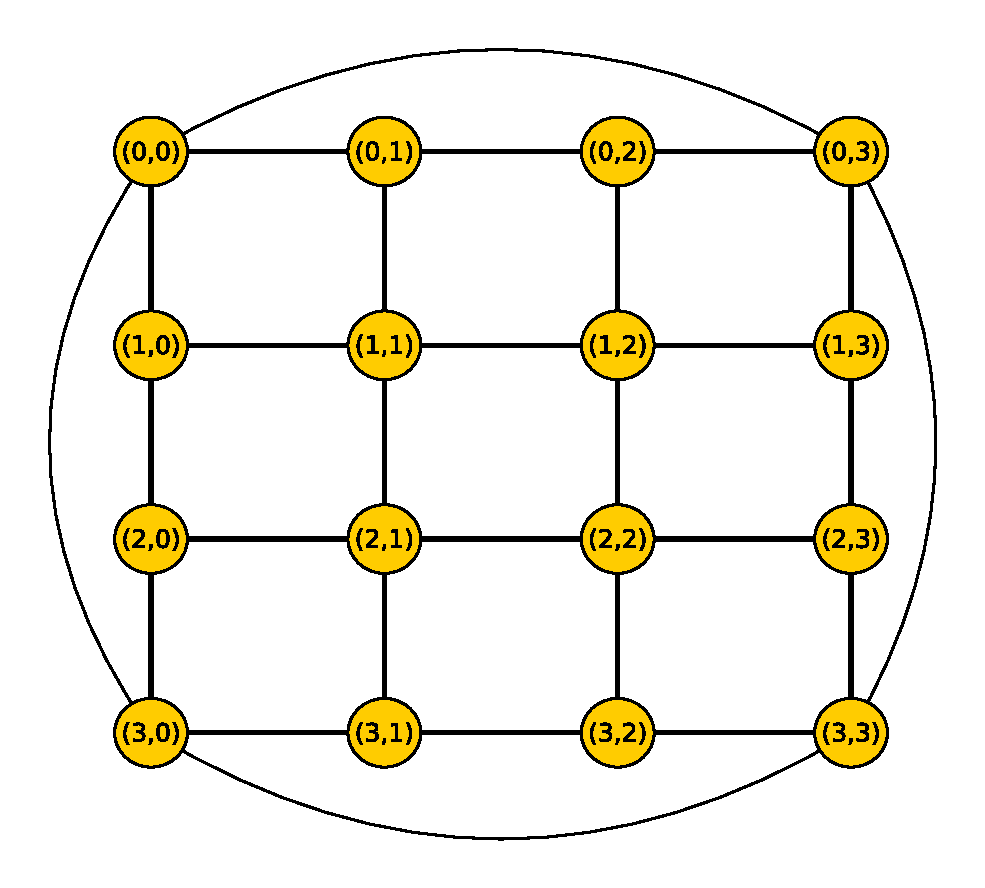
\includegraphics[scale=0.6]{exempleGrapheCelluleG33.eps}
\caption{ La grille boucl\'ee $G_{4,4}$ : elle est compos\'ee de $16$ sommets, $28$ ar\^etes et $10$ cellules. }
\label{exempleGrapheCellule} 
\end{figure}
%\FloatBarrier
% ---- figure exemple graphe cellule G_{4,4}
\begin{definition}
Une cellule est un cycle de longueur $4$ identifi\'e par les sommets $(i,j)$, $(i,j+1)$, $(i+1,j)$ et $(i+1,j+1)$ avec $i<k-1$ et $j<k'-1$. Nous notons une telle cellule $C_{i,j}$.
\end{definition}
Si $k = k' = 2$, la grille boucl\'ee $G_{2,2}$ est la cellule $C_{0,0}$.

\begin{property}
Le graphe $G_{k,k'}$ poss\`ede $k \times k'$ sommets,  $k \times (k'-1) + k' \times(k-1) + 4$  ar\^etes et $(k-1) \times (k'-1) +1$ cellules.
\end{property}

		\subsubsection{Correction des grilles boucl\'ees}
			Nous allons consid\'erer les modifications de l'ensemble des ar\^etes de $G_{k,k'}$ afin d'obtenir un line-graphe. 
La premi\`ere modification  se base uniquement par ajout d'ar\^etes et la seconde sur la suppression d'ar\^etes uniquement. 
Nous supposons que les deux op\'erations conduisent sur la m\^eme borne sup\'erieure de $DL(G_{k,k'})$.


%La grille boucl\'ee $G_{k,k'}$ ne contient aucune clique. 
%Nous appliquons l'algorithme de correction pour couvrir les sommets de ${\cal C}$  avec des cliques et que le line-graphe d\'ecoulant de cette couverture de corr\'elation soit de distance minimale. 
%Pour effectuer la correction, nous pouvons soit ajouter ou soit supprimer des ar\^etes uniquement.
%Nous simulons l'op\'eration {\em ajout uniquement} d'ar\^etes en attribuant des poids tr\`es faibles pour chaque ar\^ete ajout\'ee  et des poids tr\`es  \'elev\'es pour chaque ar\^ete supprim\'ee. De m\^eme, l'op\'eration  {\em suppression uniquement} d'ar\^etes se r\'ealise en attribuant des poids tr\`es faibles pour chaque ar\^ete supprim\'ee et des poids tr\`es  \'elev\'es pour chaque ar\^ete ajout\'ee.
%Nous allons d\'etailler les op\'erations d'ajout et de suppression d'ar\^etes pendant l'algorithme de correction. 

%Soient la fonction de co\^ut {\em ajout} qui ajoute uniquement des ar\^etes et la fonction de co\^ut {\em suppression} qui supprime uniquement des ar\^etes. 
%Nous allons d\'etailler les op\'erations d'ajout et de suppression d'ar\^etes pendant l'algorithme de correction. 

\subsubsubsection{Modification par {\em ajout d'ar\^etes uniquement}}
Soit le graphe $G_{k,k'}$ contenant $k \times k' + 1$ cellules.
Pour transformer chaque cellule en cliques comme cela est illustr\'e dans la figure \ref{exempleCorrectionGrapheCelluleAvecAjout}, nous ajoutons $2$ ar\^etes.
Nous consid\'erons le sommet $(0,0)$ contenu dans les cellules $C_{0,0}$ et $C_{k-1,k'-1}$.
Nous ajoutons $2$ ar\^etes dans $C_{0,0}$ et $C_{k-1,k'-1}$. Les cellules deviennent des cliques $K_4$. 
\newline
L'ar\^ete $\{(i,j+1),(i+1,j)\}$ appartient aux cellules  $C_{i,j}$ et  $C_{i,j+1}$.
Or cette ar\^ete est d\'ej\`a couverte par une clique $K_4$ de la cellule $C_{i,j}$.
Alors nous ne pouvons pas ajouter d'ar\^etes dans la cellule $C_{i,j+1}$.
 L'ar\^ete $\{(i,j+1),(i,j+2)\}$ forme une clique $K_2$.
 Le sommet $(i,j+1)$ est couvert par une clique $K_4$ et une clique $K_2$. 
Le sommet $(i+1,j)$ est aussi couvert par une clique $K_4$ et une clique $K_2$ parce que les cellules $C_{i,j}$ et  $C_{i+1,j}$ partagent l'ar\^ete $\{(i+1,j),(i+1,j+1)\}$  et cette ar\^ete forme une clique $K_4$ avec la cellule $C_{i,j}$.
Les cellules $C_{i,j}$ et  $C_{i+1,j+1}$ ne partagent que le sommet  $(i+1,j+1)$. En plus les ar\^etes  $\{(i+1,j+1),(i+2,j+1)\}$ de  $C_{i+1,j}$ et  $\{(i+1,j+1),(i+1,j+2)\}$ de $C_{i,j+1}$ ne sont pas couvertes par une clique $K_4$. Nous pouvons alors transformer $C_{i+1,j+1}$ en une clique $K_4$  en ajoutant $2$ ar\^etes.
\newline
Ainsi, dans des cellules successives en lignes (avec $k$) ou en colonnes (avec $k'$), nous ajoutons des ar\^etes dans $\lceil \frac{k \times k'}{2} \rceil  + 1$ cellules. 
L'ar\^ete  d'une cellule qui n'est pas contenue par une clique $K_4$ forme une clique $K_2$.
Les cellules ayant un seul sommet en commun sont transform\'ees en des cliques $K_4$. 
\newline
\`A la fin  de la correction, la grille boucl\'ee $G_{k,k'}$ est partitionn\'ee en des cliques finies $K_4$ et $K_2$.
Dans cette construction, on remarque que chaque sommet est couvert par $2$ cliques. De cette construction d\'ecoule le lemme suivant :

\begin{lemma}
La distance line d'un graphe cellule $G_{k,k'}$ avec l'op\'eration  {\em ajout uniquement} est 
\begin{equation}
DL(G_{k,k'}) \le k \times k' +3 
\end{equation}
\end{lemma}

% ---- figure exemple correction graphe cellule G_{4,4}
\begin{figure}[htb!] 
\centering
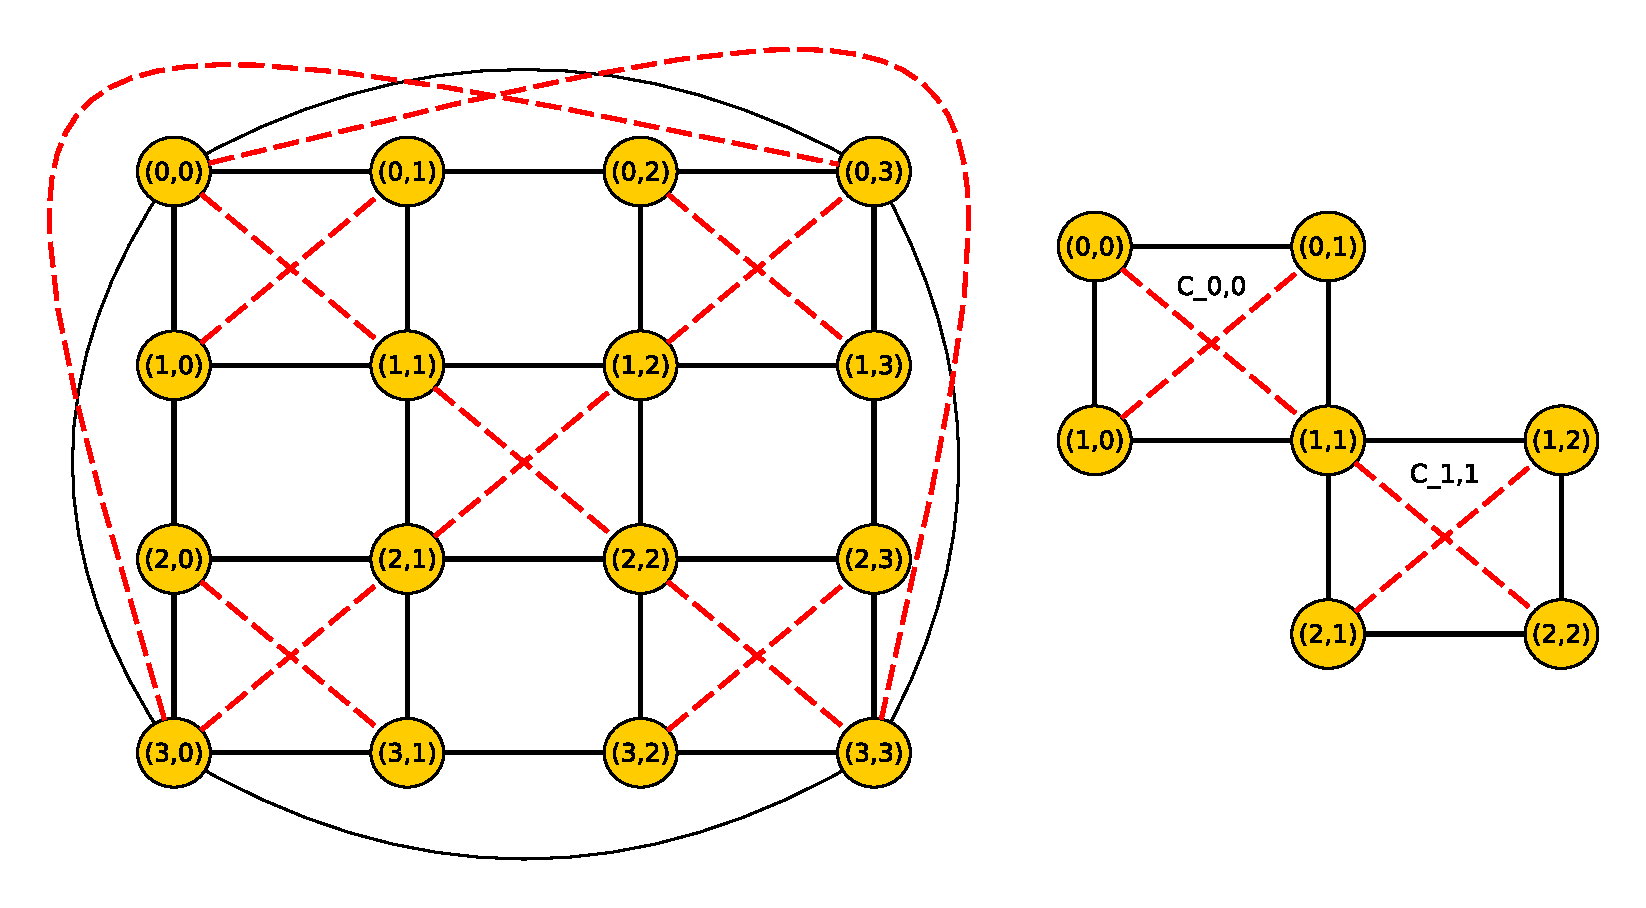
\includegraphics[scale= 0.6]{exempleGrapheCelluleAjoutG33.eps}
\caption{ La grille boucl\'ee $G_{4,4}$ : elle est compos\'ee de $16$ sommets, $33$ ar\^etes. Il contient $4$ cliques $K_{2}$ et $6$ cliques $K_4$. Les ar\^etes ajout\'ees sont les traits de couleur rouge.}
\label{exempleCorrectionGrapheCelluleAvecAjout}
\end{figure}
% ---- figure exemple correction graphe cellule G_{4,4}
Dans la figure \ref{exempleCorrectionGrapheCelluleAvecAjout}, nous r\'ealisons la correction de distance line $DL(G_{4,4})  \le 12$ en transformant les cellules partageant un sommet en cliques $K_4$. C'est le cas des cellules $C_{1,2}$ et  $C_{0,2}$ qui ont le sommet $(1,2)$ en commun. 
Les ar\^etes partag\'ees entre deux cellules ont un des sommets couvert par une clique $K_2$ et l'autre sommet couvert par une clique $K_4$. Tel est le cas avec le sommet $(3,2)$ qui forme l'ar\^ete $\{(2,2),(3,2)\}$ et cette ar\^ete est contenue par une clique $K_4$.






%
%L'ar\^ete $\{(0,1),(1,1)\}$ appartient aux cellules  $C_{0,0}$ et  $C_{0,1}$. Or cette ar\^ete est d\'ej\`a couverte par une clique $K_4$ de la cellule $C_{0,0}$. Alors nous ne pouvons pas ajouter d'ar\^etes dans la cellule $C_{0,1}$. L'ar\^ete $\{(0,1),(0,2)\}$ forme une clique $K_2$. Le sommet $(0,1)$ est couvert par une clique $K_4$ et une clique $K_2$. 
%Le sommet $(1,0)$ est aussi couvert par une clique $K_4$ et une clique $K_2$ parce que les cellules $C_{0,0}$ et  $C_{1,0}$ partagent l'ar\^ete $\{(1,0),(1,1)\}$  et cette ar\^ete forme une clique $K_4$ avec la cellule $C_{0,0}$.
%Les cellules $C_{0,0}$ et  $C_{1,1}$ ne partagent que le sommet  $(1,1)$. En plus les ar\^etes  $\{(1,1),(2,1)\}$ de  $C_{1,0}$ et  $\{(1,1),(1,2)\}$ de $C_{0,1}$ ne sont pas couverts par une clique $K_4$. Nous pouvons alors transformer $C_{1,1}$ en une clique $K_4$  en ajoutant $2$ ar\^etes .
%\newline
%Ainsi, dans des cellules successives en lignes (avec $k$) ou en colonnes (avec $k'$), nous ajoutons des ar\^etes dans une cellule sur deux. 
%%Une ar\^ete d'une cellule dans laquelle nous n'avons pas ajout\'e d'aretes devient une clique $K_2$. 
%L'ar\^ete  d'une cellule qui n'est pas contenue par une clique $K_4$ forme une clique $K_2$.
%Les cellules ayant un seul sommet en commun sont transform\'ees en des cliques $K_4$. 
%\newline
%\`A la fin  de la correction, la grille boucl\'ee $G_{k,k'}$ est partitionn\'e en des cliques $K_4$ et $K_2$.
%La distance de correction entre $G_{k,k'}$ et $L(G_{k,k'})$ est de $DC_{k,k'} = 2 \times (\lceil \frac{k \times k'}{2} \rceil  + 1)$ et cette distance est minimale.
%\begin{lemma}
%La distance line d'un graphe cellule $G_{k,k'}$ avec l'op\'eration  {\em ajout uniquement} est 
%\begin{equation}
%DL(G_{k,k'}) \le k \times k' +3 
%\end{equation}
%\end{lemma}
%\begin{proof}
%comment prouver la borne superieure?
%\end{proof}
%
%% ---- figure exemple correction graphe cellule G_{3,3}
%\begin{figure}[htb!] 
%\centering
%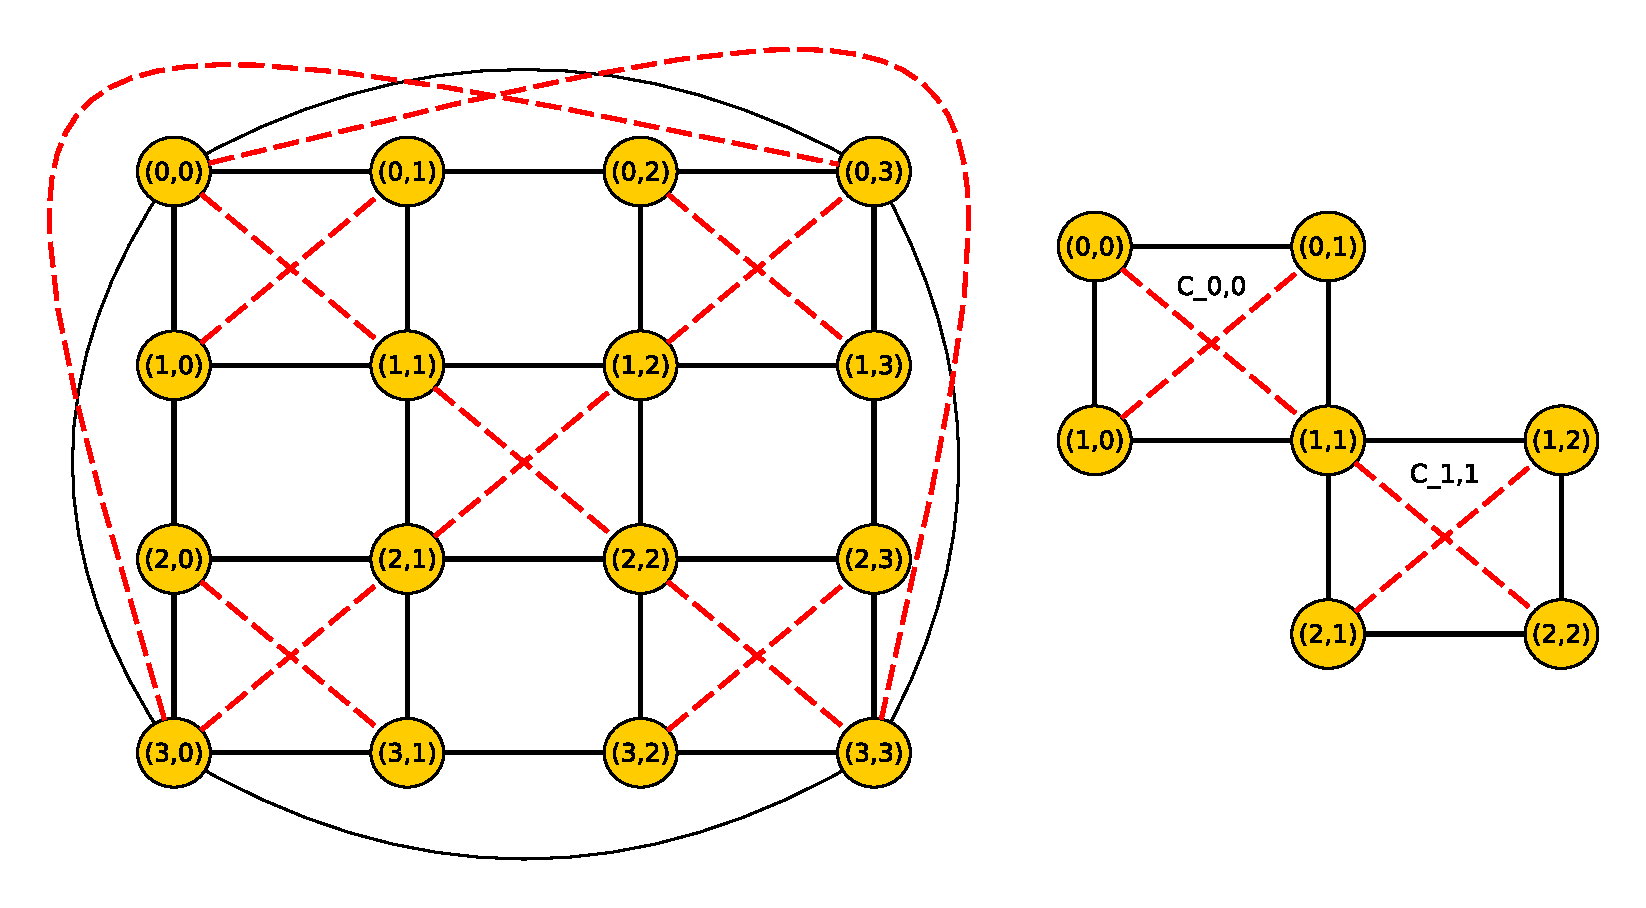
\includegraphics[scale= 0.7]{exempleGrapheCelluleAjoutG33.eps}
%\caption{ La grille boucl\'ee $G_{4,4}$ : il est compos\'e de $16$ sommets, $33$ ar\^etes. Il contient $4$ cliques $K_{2}$ et $6$ cliques $K_4$. Les ar\^etes ajout\'ees sont les traits de couleur rouge.}
%\label{exempleCorrectionGrapheCelluleAvecAjout}
%\end{figure}
%% ---- figure exemple correction graphe cellule G_{3,3}
%Dans la figure \ref{exempleCorrectionGrapheCelluleAvecAjout}, nous r\'ealisons la correction de distance line $DL(G_{4,4})=12$ minimale en transformant les cellules partageant un sommet en cliques $K_4$. C'est le cas des cellules $C_{1,2}$ et  $C_{0,2}$ qui ont le sommet $(1,2)$ en commun. 
%Les ar\^etes partag\'ees entre deux cellules ont un des sommets couvert par une clique $K_2$ et l'autre sommet couvert par une clique $K_4$. Tel est le cas avec le sommet $(3,2)$ qui forme l'ar\^ete $\{(2,2),(3,2)\}$ et cette ar\^ete est contenue par une clique $K_4$.

\subsubsubsection{Modification par {\em suppression d'ar\^etes uniquement}}
\label{modificationSuppressionAretesUniquement}
Soit le graphe $G_{k,k'}$ contenant $k \times k' + 1$ cellules.
Nous supprimons les ar\^etes \\ $[\{(0,0),(k-1,0) \},  \{(0,0),(0, k'-1) \}, \{(k-1,0),(k-1,k'+1) \}]$ de la  cellule $C_{k-1,k'-1}$. Cette cellule contient uniquement  l'ar\^ete $\{(0,k'-1),(k-1,k'-1) \}$ et cette ar\^ete forme la clique $K_2$.
Nous supprimons \'egalement les ar\^etes $\{(0,k'-2),(0,k'-1)\}$ et $\{(k-2,k'-1),(k-1,k'-1) \}$  incidentes respectivement aux sommets $(0,k'-1)$ et $(k-1,k'-1)$ de sorte que ces sommets soient couverts par deux cliques $K_2$.
Les sommets de degr\'e minimums $(0,0)$, $(k-1,0)$. Ils sont couverts par deux cliques $K_2$ c'est-\`a-dire $\{(0,0),(1,0)\}$ et $\{(k-2,0) ,(k-1,0)\}$.
\newline
Consid\'erons les sommets de degr\'e $4$. Soit $(i,j)$ un tel sommet.
Pour former une bipartition autour de ce sommet, nous allons supprimer $2$ ar\^etes. Chaque ar\^ete appartient \`a deux cellules voisines. Dans notre cas, nous supprimons l'ar\^ete $\{(i-1, j), (i,j)\}$ entre les cellules $C_{i-1,j-1}$ et $C_{i-1,j}$ et aussi l'ar\^ete $\{(i,j), (i+1,j)\}$ entre les cellules $C_{i,j-1}$ et $C_{i,j}$. Ces sommets sont couverts aussi par des cliques $K_2$.
\newline
Les ar\^etes incidentes \`a un sommet de degr\'e $3$ et n'\'etant pas des cliques $K_2$ sont aussi supprim\'ees.
\newline
\`A la fin de l'algorithme de correction, la couverture de corr\'elation ne contient que des cliques $K_2$.
Le graphe $G_{k,k'}$ est un cycle hamiltonien de taille $(k \times k'+1) + k' + 1$.
La distance de correction entre $G_{k,k'}$ et $L(G_{k,k'})$ est $DC_{k,k'} = k \times k' +3 $ et cette distance est minimale.

\begin{lemma}
La distance line  d'une grille boucl\'ee $G_{k,k'}$ avec l'op\'eration {\em suppression uniquement} d'ar\^etes est 
\begin{equation}
\label{borneSuperieureDL}
DL(G_{k,k'}) = k \times k' +3 
%DL_{supp}(G_{k,k'}) = k \times (k' +1) ===> cela correspond a quoi?
\end{equation}
\end{lemma}

% ---- figure exemple correction graphe cellule G_{3,3}
\begin{figure}[htb!] 
\centering
\includegraphics[scale = 0.7]{exempleGrapheCellulesSuppressionG33.eps}
\caption{ La grille boucl\'ee $G_{4,4}$ : elle est compos\'ee de $16$ sommets, $16$ ar\^etes et $16$ cliques $K_2$. Les ar\^etes supprim\'ees sont les traits en pointill\'ees rouges }
\label{exempleCorrectionGrapheCelluleAvecSuppression}
\end{figure}
%\FloatBarrier
% ---- figure exemple correction graphe cellule G_{3,3}
Une illustration de la correction avec l'op\'eration {\em suppression uniquement} est faite avec la grille $G_{4,4}$ dans la figure \ref{exempleCorrectionGrapheCelluleAvecSuppression}.
La grille $G_{4,4}$ poss\`ede $ k \times k' = 16$ cliques $K_2$ et $12$ ar\^etes sont supprim\'ees.
\newline

% conclusion
%Nous avons d\'etermin\'e les distances line th\'eoriques selon les fonctions de co\^ut lors de la correction de sommets de graphes cellules. Nous allons v\'erifier si les distances line obtenues exp\'erimentalement convergent vers les distances line th\'eoriques.
{\bf Conclusion} :
nous avons d\'etermin\'e deux types de modifications d'ar\^etes qui ont une borne sup\'erieure de la distance line pour chaque op\'eration. En revanche, les cliques formant la couverture de corr\'elation sont diff\'erentes selon la modification. Dans la modification {\em ajout d'ar\^etes uniquement}, le grille boucl\'e $G_{k.k'}$ contient des cliques $K_4$ et $K_2$ alors que  $G_{k.k'}$ ne contient que des cliques $K_2$ dans la {\em suppression d'ar\^etes uniquement}. 



%Nous remarquons que ces bornes  sont identiques. La distance line th\'eorique est alors born\'ee par $k \times k' +3$ quelque soit l'op\'eration de correction effectu\'ee.
%Nous allons v\'erifier si les distances de correction, obtenues apr\`es la correction des grilles boucl\'ees,  convergent vers la borne des distances line th\'eoriques.
%
%
%

	\subsection{Protocole d'exp\'erimentation sur les grilles boucl\'ees}
		Nous allons comparer cette borne sup\'erieure de l'\'equation \ref{borneSuperieureDL} avec les distances de correction obtenues par l'algorithme de correction.
\newline
Consid\'erons $G_{k,k'}$ une grille boucl\'ee dans laquelle le nombre de sommets par lignes est identique le nombre de sommets par colonnes ($k = k'$). Nous le notons $G_k$.
\newline
Nous construisons $48$ grilles boucl\'ees  contenant chacune $k \times k +1$ cellules, avec $k \in \{2,\cdots,98\}$ un nombre pair.
Dans chaque graphe $G_k$, nous ex\'ecutons   $50$ fois notre couple d'algorithmes avec chaque modification d'ar\^etes et la distance de correction obtenue est compar\'ee avec la borne sup\'erieure (\'equation \ref{borneSuperieureDL}).
\newline

Soient $\phi^{+}(u,v)$ le co\^ut de l'op\'eration {\em ajouter une ar\^ete} et 
$\phi^{-}(u,v)$ le poids de l'op\'eration {\em supprimer une ar\^ete} (voir section \ref{algorithmeCorrection}). 
\newline
La modification {\em ajout d'ar\^etes uniquement} est telle que 
\begin{itemize}
	\item L'ajout d'ar\^etes a un co\^ut  $\phi^{+}(u,v) = 1$,
	\item La suppression d'ar\^etes a un co\^ut  $\phi^{-}(u,v) = 10$.
\end{itemize}
Quant \`a la modification {\em suppression d'ar\^etes uniquement}, elle se d\'efinit comme suit :
\begin{itemize}
	\item L'ajout d'ar\^etes a un co\^ut  $\phi^{+}(u,v) = 10$.
	\item La suppression d'ar\^etes a un co\^ut  $\phi^{-}(u,v) = 1$.
\end{itemize}
Nous allons comparer l'\'evolution des distances de correction des $48$ graphes en fonction la borne sup\'erieure pour chaque modification r\'ealis\'ee.

%
%Consid\'erons $G_{k,k'}$ une grille boucl\'ee dans lequel le nombre de sommets par lignes est identique le nombre de sommets par colonnes ($k = k'$). Nous notons $G_k$ pour d\'esigner $G_{k,k'}$ et $G_k$ contient $k \times k +1$ cellules.
%Nous construisons $48$ grilles boucl\'ees dans lesquels chaque graphe contient $k \times k +1$ cellules $k \in \{2,\cdots,98\}$.
%Dans chaque graphe $G_k$, nous ex\'ecutons  notre couple d'algorithmes $50$ fois puis nous r\'ecup\'erons la distance de correction  minimale entre $G_k$ et les line-graphes $L(G_k)$ propos\'ees.
%Nous utilisons la   distance de correction  minimale parce qu'il est impossible de trouver la bonne permutation qui minimise cette distance \`a cause de la combinatoire factorielle de l'ensemble $\cal C$.
%\newline
%Soient $\phi^{+}(u,v)$ le poids de l'op\'eration {\em ajouter une ar\^ete} et $\phi^{-}(u,v)$ le poids de l'op\'eration {\em supprimer une ar\^ete}. 
%L'op\'eration {\em ajout uniquement} d'ar\^etes est telle que  $\phi^{+}(u,v) = 1$ pour l'ajout de l'ar\^ete $(u,v)$ et $\phi^{-}(u,v) = 10$ pour la suppression de l'ar\^ete $(u,v)$.
%De m\^eme,  L'op\'eration {\em suppression uniquement} d'ar\^etes est telle que  $\phi^{+}(u,v) = 10$ pour l'ajout de l'ar\^ete $(u,v)$ et $\phi^{-}(u,v) = 1$ pour la suppression de l'ar\^ete $(u,v)$.
%L'objectif de notre exp\'erimentation est de comparer l'\'evolution des distances de correction obtenues apr\`es la correction des grilles boucl\'ees par rapport aux bornes sup\'erieures des distances line th\'eoriques. 

%Nous d\'efinissons les fonctions de co\^ut {\em ajout} et {\em suppression} comme suit :
%\begin{enumerate}[label = (\alph*)]
%%\item {\em unitaire} : ajouter et supprimer une ar\^ete ont un poids $1$ ($\phi^{+} = \phi^{-} = 1$).
%\item {\em ajout} : nous donnons un poids minimal \`a l'op\'eration ``ajouter d'ar\^etes''. Ainsi nous attribuons un poids $\phi^{+} = 1$ pour l'ajout d'ar\^etes et un poids $\phi^{-} = 10$ pour la suppression d'ar\^etes.
%\item {\em suppression} : Ici nous faisons l'op\'eration inverse en donnant un poids maximal \`a l'op\'eration d'ajout d'ar\^etes. Ainsi, l'ajout d'une ar\^ete a un poids $\phi^{+} = 10$ alors que la suppression a un poids $\phi^{-} = 1$.
%\end{enumerate}
%L'objectif de notre exp\'erimentation est de comparer les distances lines th\'eoriques avec celles obtenus avec l'utilisation des fonctions de co\^uts mentionn\'ees ci-dessus.


%Nous allons comparer les diff\'erentes fonctions de co\^ut en utilisant les distances line calcul\'ees. Les courbes croissantes dans les figures \ref{priorAjout1Ajout10}, \ref{priorAjout1Supp10} et \ref{priorAjout1Supp1} s'explique par le fait que les distances line sont rang\'ees par ordre croissant.
	\subsection{Analyse des r\'esultats}
		% ---- figure comparaison_distances_line_graphes_cellules_k_2x50
%\begin{figure}[htb!] 
%\centering
%\includegraphics[scale = 0.25]{comparaison_distances_line_graphes_cellules_k_2x50.jpeg}
%\caption{Comparaison de distances lines th\'eoriques et calcul\'ees selon des fonctions de co\^ut {\em suppression} et  {\em ajout}.
%La figure $(a)$ d\'esigne la comparaison entre les distances de correction et la borne sup\'erieure de l'\'equation \ref{borneSuperieureDL} avec la modification {\em ajout d'ar\^etes uniquement}, 
%La figure $(c)$ d\'esigne la comparaison entre les distances de correction et la borne sup\'erieure de l'\'equation \ref{borneSuperieureDL} avec la modification {\em suppression d'ar\^etes uniquement}, 
%La figure $(b)$ compare le pourcentage d'ar\^etes supprim\'ees  dans les graphes boucl\'ees avec celui de la borne sup\'erieure de l'\'equation \ref{borneSuperieureDL} dans la modification {\em ajout d'ar\^etes uniquement}, 
%La figure $(d)$ compare le pourcentage d'ar\^etes supprim\'ees  dans les graphes boucl\'ees avec celui de la borne sup\'erieure de l'\'equation \ref{borneSuperieureDL} dans la modification {\em suppression d'ar\^etes uniquement},
%La figure $(e)$ compare les distances de correction entre les diff\'erentes modifications.
%}
%\label{comparaison_distances_line_graphes_cellules_k_2x50}
%\end{figure}
%\FloatBarrier
\begin{figure}[htb!] 
\centering
\includegraphics[scale = 0.25]{comparaison_distances_line_graphes_cellules_k_2x50.jpeg}
\caption{Comparaison entre la borne sup\'erieure de la distance line et les distances de correction calcul\'ees selon des fonctions de co\^ut {\em suppression} et  {\em ajout} : 
la figure $(a)$ d\'esigne la comparaison entre les distances de correction et la borne sup\'erieure de l'\'equation \ref{borneSuperieureDL} avec la modification {\em ajout d'ar\^etes uniquement}, 
la figure $(c)$ d\'esigne la comparaison entre les distances de correction et la borne sup\'erieure de l'\'equation \ref{borneSuperieureDL} avec la modification {\em suppression d'ar\^etes uniquement}, 
la figure $(b)$ compare le pourcentage d'ar\^etes supprim\'ees  dans les graphes boucl\'ees avec celui de la borne sup\'erieure de l'\'equation \ref{borneSuperieureDL} dans la modification {\em ajout d'ar\^etes uniquement}, 
la figure $(d)$ compare le pourcentage d'ar\^etes supprim\'ees  dans les graphes boucl\'ees avec celui de la borne sup\'erieure de l'\'equation \ref{borneSuperieureDL} dans la modification {\em suppression d'ar\^etes uniquement},
la figure $(e)$ compare les distances de correction entre les diff\'erentes modifications.
}
\label{comparaison_distances_line_graphes_cellules_k_2x50}
\end{figure}
%\FloatBarrier
% ---- figure comparaison_distances_line_graphes_cellules_k_2x50


Notre objectif est de pr\'esenter les variations des distances de correction par rapport \`a la borne sup\'erieure de la distance line pour chaque modification r\'ealis\'ee sur les graphes pendant l'algorithme de correction. Pour ce faire, nous regroupons notre analyse en $5$ exp\'erimentations.
\newline

Les deux premi\`eres exp\'erimentations comparent les distances de correction avec la borne sup\'erieure pour la modification {\em ajout d'ar\^etes uniquement} (figure \ref{comparaison_distances_line_graphes_cellules_k_2x50} (a) et 
pour la modification {\em suppression d'ar\^etes uniquement} figure \ref{comparaison_distances_line_graphes_cellules_k_2x50} (c).
Nous constatons que les courbes des distances de correction et celle de la borne sup\'erieure sont croissantes. 
La courbe de la borne sup\'erieure, d\'esign\'ee par $borneSup$ dans les graphiques $(a)$ et $(c)$, \'evolue lentement par rapport aux courbes des distances et l'\'ecart entre ces courbes croit lin\'eairement. 
Pour comprendre cet \'ecart croissant, nous v\'erifions le pourcentage d'ar\^etes  supprim\'ees pour chaque modification.  Ce sont les deux autres exp\'erimentations faites et repr\'esent\'ees par la figure 
\ref{comparaison_distances_line_graphes_cellules_k_2x50} (b) pour la modification {\em ajout d'ar\^etes uniquement} et
 la figure \ref{comparaison_distances_line_graphes_cellules_k_2x50} (d) pour la modification 
{\em suppression d'ar\^etes uniquement}. 
En effet, nous avons choisi les ar\^etes supprim\'ees parce que le nombre d'ar\^etes est d\'ej\`a connu c'est-\`a-dire $0$ pour l'ajout uniquement et la borne sup\'erieure pour la suppression uniquement. 
\newline
Nous remarquons que les ar\^etes   de $G_k$ supprim\'ees avoisinent en moyenne de
$40\%$ quand le nombre $k$ de cellules est faible ($k \le 14$) dans la modification {\em ajout ar\^etes uniquement}. Au d\'el\`a de $ k > 14 $, une ar\^ete sur deux du graphe $G_{k}$ est supprim\'ee. La courbe  $aretes\_supprimees\_ajout\_1$ dans le graphique $(b)$ repr\'esente le pourcentage d'ar\^etes supprim\'ees.  
En effet, nous expliquons ces chiffres  par l'ajout d'ar\^etes entre des sommets de cellules voisines et ces sommets ne sont pas partag\'es entre les cellules voisines. Ces ar\^etes ajout\'ees impliquent la suppression des ar\^etes de $G_k$ parce que la partition $\pi_s$ (voir section \ref{algorithmeCorrection}) des ar\^etes \`a supprimer pendant la compression n'est pas vide et contient des ar\^etes de $G_k$ en g\'en\'eral. Ainsi ces ar\^etes provoquent l'abandon des ar\^etes diagonales  ajout\'ees \`a partir du sommet commun entre des cellules comme indiqu\'e dans l'exemple du graphe $G_{4,4}$ dans la figure \ref{exempleCorrectionGrapheCelluleAvecAjout}.
\newline
En ce qui concerne la modification {\em suppression d'ar\^etes uniquement}, les ar\^etes supprim\'ees proviennent aussi des cellules voisines. 
Dans les cellules partageant un sommet, l'algorithme ajoute g\'en\'eralement une ar\^ete diagonale \`a partir de ce sommet commun dans une seule cellule. Les ar\^etes diagonales ajout\'ees sont responsables de l'augmentation de la distance de correction (courbe {\em dc\_supp\_1} dans le graphique $(c)$).
Pour des cellules partageant une ar\^ete, l'algorithme supprime certaines ar\^etes communes comme indiqu\'e dans la section \ref{modificationSuppressionAretesUniquement}. Les autres ar\^etes communes non supprim\'ees sont dues \`a la pr\'esence des ar\^etes diagonales. Cela explique pourquoi nous avons en moyenne $50\%$ des ar\^etes de $G_k$ qui sont supprim\'ees dans le graphique $(d)$. Ce pourcentage est identique \`a celui des ar\^etes supprim\'ees de la borne sup\'erieure lorsque le nombre de cellules devient \'elev\'e $k \ge 18$ et il ne signifie pas que l'algorithme de correction supprime les ar\^etes de la section \ref{modificationSuppressionAretesUniquement}.
\newline
Par ailleurs, les courbes {\em dc\_ajout\_1} de la modification d'{\em ajout d'ar\^etes uniquement} et celle {\em dc\_supp\_1}  de la modification {\em suppression d'ar\^etes uniquement} ont les m\^emes tendances et sont superpos\'ees (figure $(e)$) parce que  dans la modification d'{\em ajout}, l'algorithme ajoute la m\^eme proportion d'ar\^etes qu'il supprime dans  la modification {\em suppression}. 
\newline

\vspace{-0.25cm}
{\bf Conclusion} :   
l'exp\'erimentation montre que le line-graphe $L(G_k)$ propos\'e par l'algorithme de correction pour un $k$ donn\'ee est identique en terme de distance de correction quelle que soit la modification r\'ealis\'ee comme illustre la figure \ref{comparaison_distances_line_graphes_cellules_k_2x50}(e).
Toutefois, les graphes corrig\'es ne sont pas optimaux en terme de distances de correction parce que l'algorithme priorise dans certains cas les modifications {\em ajout d'ar\^etes uniquement} et {\em suppression uniquement} et cela leur permet d'atteindre des minimums locaux. Cependant le minimum global n'est pas atteint g\'en\'eralement. 


	\subsection{Conclusion de l'exp\'erimentation 3}
		
Les grilles boucl\'ees ont la particularit\'e d'avoir des ar\^etes qui ne peuvent \^etre partitionn\'ees en cliques. 
Nous avons d\'ecrit la construction de ces graphes et nous d\'efinissons deux m\'ethodes pour les corriger. La premi\`ere m\'ethode est la modification d'{\em ajout uniquement} qui consiste \`a ajouter uniquement des ar\^etes  et la seconde m\'ethode est la modification {\em suppression uniquement} qui supprime uniquement des ar\^etes des grilles boucl\'ees. 
Avec ces m\'ethodes, nous avons trouv\'e une borne sup\'erieure unique de la distance line des  grilles boucl\'ees et nous avons compar\'e cette borne sup\'erieure avec les distances de correction obtenues apr\`es l'algorithme de correction.
\newline
Nous remarquons que les distances de correction varient tr\`es peu entre les modifications {\em ajout uniquement} et {\em suppression uniquement}.  Les graphes corrig\'es n'ont pas de distances de corrections optimales parce que l'algorithme supprime des ar\^etes pendant la modification {\em ajout d'ar\^etes uniquement} et ajoute des ar\^etes pendant la modification {\em suppression uniquement}.  

%et ces distances ne convergent pas vers les distances th\'eoriques parce qu'il ajoute des ar\^etes dans l'op\'eration {\em suppression uniquement} et supprime des ar\^etes dans l'op\'eration {\em ajout uniquement}.  Par ailleurs, les distances line th\'eoriques sont identiques quelques soient les op\'erations car les expressions litt\'erales de ces distances  ont le m\^eme d\^egre de polyn\^omes et les coefficents de ces polyn\^omes sont tr\`es proches.

%---------------------------------------------------------------------------
%------- conclusion chapitre
%---------------------------------------------------------------------------
	\section{Conclusion du chapitre \ref{chapitreEvaluation}}
		% conclusion generale 
Le chapitre \ref{chapitreEvaluation} analyse les performances de nos algorithmes de couverture et de correction selon $3$ exp\'erimentations. 

% experimentation 1
La premi\`ere exp\'erimentation consiste \`a modifier les $k$ cases de la matrice d'adjacence du line-graphe d'un r\'eseau \'electrique. Ces cases modifi\'ees sont divis\'ees en deux sous-ensembles disjoints (cases {\em fausses n\'egatives} et cases {\em fausses positives}) selon une variable $p \in [0,1]$. Si $p = 0$ alors l'ensemble des cases modifi\'ees est compos\'e que de cases  {\em fausses positives} et si $p=1$ alors nous avons que des cases {\em fausses n\'egatives}. 
Le but est de borner le nombre de cases corrig\'ees par nos algorithmes.
Ainsi, nous avons d\'efini les distances de correction et de Hamming. 
La distance de correction est le nombre minimum de cases \`a modifier dans un graphe de $k$ cases erron\'ees pour en faire un line-graphe. 
Quant \`a la distance de Hamming, elle est la diff\'erence de cases entre les matrices de line-graphe propos\'e par nos algorithmes et le line-graphe du r\'eseau \'electrique.
Nous avons compar\'e le nombre de cases corrig\'ees avec $5$ approches de correction qui sont : {\em al\'eatoire sans remise $(2c)$}, {\em degr\'e minimun sans remise $(2a)$}, {\em co\^ut minimum sans remise $(2b)$}, {\em degr\'e minimun avec remise $(1a)$}, {\em co\^ut minimum avec remise $(1b)$}. \`A chaque approche, nous avons $3$ co\^uts de modification  d'une case : {\em unitaire}, {\em ajout} et {\em suppression}.
Nous avons conclut que l'approche  {\em al\'eatoire sans remise $(2c)$} proposait des distances de correction minimales quelle que soit la repartition effectu\'ee $p$ et la fonction de co\^ut utilis\'ee. Ces distances constituent la borne sup\'erieure de la distance line quand le nombre $k$ de cases modifi\'ees est faible $k \le 5$. 
D'autre part, nous avons montr\'e que les distances de correction et de Hamming deviennent tr\`es corr\'el\'ees quand le nombre de cases modifi\'ees initiales est \'elev\'e $k > 10$. Dans ce cas o\`u $k \le 5$, le line-graphe propos\'e par l'algorithme de correction est celui de r\'eseau \'electrique. La distance de correction peut \^etre utilis\'ee comme une m\'etrique lorsque la topologie initiale du r\'eseau est inconnue.
\newline

% experimentation 2
La seconde exp\'erimentation consid\`ere que chaque case de la matrice du line-graphe est associ\'ee \`a une valeur de corr\'elation.  Les valeurs de corr\'elation sont g\'en\'er\'ees en tenant compte des distributions des valeurs de corr\'elation  du r\'eseau \'electrique d'un data center {\em Champlan}. Ces corr\'elations sont calcul\'ees avec la {\em distance de Pearson}. Les valeurs de corr\'elation dans la matrice forment la {\em matrice de corr\'elation}. Nous avons d\'efini un ensemble de seuil dans lequel chaque seuil est appliqu\'e \`a la matrice de corr\'elation pour en construire la matrice d'adjacence du graphe $G_s$. Le graphe $G_s$ contient des cases {\em fausses n\'egatives} et des cases {\em fausses positives}. 
Notre objectif est de minimiser le nombre de cases erron\'ees dans le graphe $G_s$ apr\`es l'ex\'ecution de nos algorithmes et cela n\'ecessite la s\'election d'une valeur ad\'equate du seuil. 
Nous avons consid\'er\'e l'approche de correction  {\em al\'eatoire sans remise $(2c)$} et nous avons s\'electionn\'e quatre fonctions de co\^ut : {\em unitaire}, {\em ajout}, {\em suppression} et {\em normale}. Les fonctions de co\^ut sont fonction des cases modifi\'ees par l'algorithme de correction.
Nous avons d\'eduit que le bon seuil appartient \`a l'intervalle $s \in ]0.6,0.7]$ et la fonction {\em normale} donne de bons r\'esultats pour le calcul dans les distances de correction et de Hamming.
\newline

% experimentation 3
La derni\`ere exp\'erimentation se focalise sur les graphes dans lesquelles un sommet et son voisinage ne peuvent \^etre couverts par une ou deux cliques. Un exemple de ces graphes est la famille des graphes {\em grilles boucl\'ees}. Une grille boucl\'ee de  $k$  lignes et $k'$ colonnes est compos\'ee de $(k-1 )\times (k'-1) +1$ cellules avec une cellule un graphe biparti $K_{2,2}$ non orient\'e.
Nous avons montr\'e que la correction de ces graphes peut se faire selon deux m\'ethodes (modification  {\em ajout d'ar\^etes uniquement} et {\em suppression d'ar\^etes uniquement}). Les deux modifications admettent la m\^eme borne sup\'erieure de ses distances line. 
 Notre objectif est de v\'erifier que la convergence  des distances de correction  vers la borne sup\'erieure quelque soit la modification r\'ealis\'ee. 
 Les r\'esultats obtenus montrent que les distances de correction sont invariantes peu importe les modifications et que les  graphes corrig\'es n'ont pas de distances de corrections optimales. 
 \newline


Au terme de ces $3$ exp\'erimentations, nous pouvons conclure que nos algorithmes n'ont pas un comportement optimal lorsque le mode de correction est {\em al\'eatoire sans remise}  et le seuil de corr\'elation est contenu dans l'intervalle $]0.6,0.7]$ peu importe la repartition des cases erron\'ees et la fonction de co\^ut. 
Ces conditions garantissent que la distance de correction est minimale pour des graphes ayant peu d'erreurs et le line-graphe propos\'e par l'algorithme de correction diff\`ere de peu d'ar\^etes du line-graphe cible. 
 Cependant pour la famille des graphes dont aucun sommet ne peut \^etre couvert par une clique (cas des grilles {\em boucl\'ees}),  les distances line calcul\'ees ne convergent pas vers la borne sup\'erieure d\'efinie. Toutefois, le type de correction (modifications {\em ajout uniquement} et {\em suppression uniquement}) sur ces graphes n'influencent pas les valeurs de distances de correction. 




%\section{Annexes}
%	% annexes
\label{annexe_distribution_0_9}

%{\large R\'esultats de la modification de $k \in \{1,2,3,4,5\}$ cases avec $p=0.5$ }
\begin{figure}[htb!] 
\centering
\includegraphics[width=550pt,height=580pt]{unitaire_aleatoire_sansRemise_distanceMoyenDLDH_k_1_2_3_4_5_p_05.jpeg}
\caption{ Approche de correction al\'eatoire sans remise \`a co\^ut unitaire pour $k =\{1,2,3,4,5\} $ cases modifi\'ees : La premi\`ere colonne repr\'esente la distribution des distances de correction $moy\_DC_{k,0.5}$. La seconde colonne est la distribution des distances de Hamming $moy\_DH_{k,0.5}$. La troisi\`eme colonne  est la fonction de repartition de la corr\'elation entre les distances de correction et de Hamming avec en abscisse la corr\'elation entre ces distances (correlation\_DC\_DH).  La quatri\`eme colonne est la fonction cumulative des distances de Hamming. La premi\`ere ligne est associ\'ee \`a $k=1$ case modifi\'ee, la seconde ligne \`a $k=2$ cases modifi\'ees, la troisi\`eme ligne \`a $5$ cases modifi\'ees et enfin la derni\`ere \`a $9$ cases modifi\'ees.}
\label{sansremise_unitaire_distanceMoyenDCDH_k_1_5_aleatoire_p_05} 
\end{figure}
\FloatBarrier

%{\large R\'esultats de la modification de $k \in \{6,7,8,9,\}$ cases avec $p=0.5$ }
\begin{figure}[htb!] 
\centering
\includegraphics[width=550pt,height=580pt]{unitaire_aleatoire_sansRemise_distanceMoyenDLDH_k_6_7_8_9_p_05.jpeg}
\caption{ Approche de correction al\'eatoire sans remise \`a co\^ut unitaire pour $k =\{6,7,8,9\} $ cases modifi\'ees : La premi\`ere colonne repr\'esente la distribution des distances de correction $moy\_DC_{k,0.5}$. La seconde colonne est la distribution des distances de Hamming $moy\_DH_{k,0.5}$. La troisi\`eme colonne  est la fonction de repartition de la corr\'elation entre les distances de correction et de Hamming avec en abscisse la corr\'elation entre ces distances (correlation\_DL\_DH).  La quatri\`eme colonne est la fonction cumulative des distances de Hamming. La premi\`ere ligne est associ\'ee \`a $k=1$ case modifi\'ee, la seconde ligne \`a $k=2$ cases modifi\'ees, la troisi\`eme ligne \`a $5$ cases modifi\'ees et enfin la derni\`ere \`a $9$ cases modifi\'ees.}
\label{sansremise_unitaire_distanceMoyenDCDH_k_6_9_aleatoire_p_05} 
\end{figure}





	%---- conclusion et persectives
%	\input@path{conclusionGeneraleV1}
	
\chapter{Conclusion g\'en\'erale}

\section{Conclusion}
	Les algorithmes pr\'esent\'es dans ce document s'inscrivent dans le cas g\'en\'eral de l'\'etude de d\'ecouverte de topologie. La probl\'ematique \`a laquelle nous avons tent\'e de repondre est :
\'etant donn\'es un ensemble de mesures physiques souvent erron\'ees et de lois physiques sur les liens d'un r\'eseau de flots, est il possible de d\'ecouvrir la topologie d'un r\'eseau \'energ\'etique dans lequel les mesures sont extraites?
Nous avons restreint le r\'eseau \'energ\'etique \`a un r\'eseau \'electrique parce que l'entreprise {\em DCbrain SAS}, \`a l'origine de la th\`ese, avait de soucis de sch\'emas \'electriques pendant l'\'etude \'energ\'etique d'un data center. Elle a constat\'e que le sch\'ema \'electrique n'\'etait pas mis \`a jour  entre deux maintenances successives.
Pour repondre alors \`a ce probl\`eme, nous avons proc\'ed\'e en $4$ \'etapes.
\newline

La premi\`ere \'etape a \'et\'e de consid\'erer les mesures comme des s\'eries temporelles ensuite de s\'electionner les grandeurs physiques pr\'esentes dans le r\'eseau et de d\'efinir des lois de conservation adapt\'ees aux grandeurs de ce r\'eseau. Ensuite nous avons mod\'elis\'e le r\'eseau par un graphe de flots dans lequel les mesures sont les flots, les sommets sont les \'equipements, les arcs sont les c\^ables \'electriques et le graphe est un DAG sans circuit.
\newline

Dans la seconde \'etape, nous avons remarqu\'e, sur certains \'equipements adjacents dont nous connaissons leurs mesures, que les courbes des mesures ont les m\^emes comportements aux m\^emes instants de temps. Nous avons d\'ecid\'e de comparer  les comportements des s\'eries temporelles en supposant que les arcs, d'o\`u proviennent les mesures, ont une extr\'emit\'e commune si leurs s\'eries temporelles ont des comportements similaires. Nous avons list\'e les diff\'erentes m\'ethodes de comparaison et nous avons choisi la distance de Pearson parce qu'elle est une m\'etrique, 
elle est de complexit\'e lin\'eaire et 
elle ne traite pas le d\'ecalage temporel. 
Les valeurs de distances aussi appel\'ees coefficients de similarit\'e appartiennent \`a $[0,1]$. Un coefficient proche de $1$ signifie qu'il existe une extr\'emit\'e commune entre une paire d'arcs. En testant la distance de Pearson sur un sous-r\'eseau r\'eel du datacenter {\em Champlan}, nous avons constat\'e des erreurs dans les coefficients de similarit\'e c'est-\`a-dire un coefficient proche de $0$ alors qu'il n'existe aucune extr\'emit\'e commune entre une paire d'arcs. Ces erreurs  sont dues aux m\'ecanismes de fonctionnement, aux donn\'ees et aussi \`a la distance de Pearson. 
Les coefficients de similarit\'e forment la matrice de corr\'elation et le graphe associ\'e \`a cette matrice est le {\em graphe de corr\'elation}. Si cette matrice ne contient aucune erreur alors le graphe de corr\'elation est le line-graphe du graphe non orient\'e sous-jacent au DAG du r\'eseau \'electrique. 
\newline

Le troisi\`eme \'etape a montr\'e que le line-graphe a une partition unique de son ensemble d'ar\^etes en cliques appel\'e la {\em couverture de corr\'elation} sauf en cas d'ambigu\"{i}t\'es o\`u nous utilisons les mesures \'electriques et la fonction $Verif-correl$ (voir section \ref{VerifCorrel}) pour d\'eterminer la bonne partition au voisinage d'un sommet ambigu. 
Nous avons propos\'e  l'algorithme de couverture qui retourne la couverture de corr\'elation du graphe de corr\'elation si celui-ci ne contient aucune erreur. 
Dans le cas contraire, les sommets n'\'etant pas couverts dans la couverture de corr\'elation sont corrig\'es avec l'algorithme de correction. La correction consiste alors \`a supprimer et \`a ajouter des ar\^etes incidentes \`a un sommet \`a corriger de telle sorte que le partitionnement de son voisinage forme deux cliques et le co\^ut de modification des ar\^etes incidentes de ce sommet soit de co\^ut minimum. 
Nous avons propos\'e, \`a partir de la couverture de corr\'elation, une m\'ethode pour construire le graphe non orient\'e  sous-jacent au DAG et aussi une heuristique pour orienter les ar\^etes de ce graphe. Cependant cette heuristique ne donne pas une solution optimale.
\newline

Dans la quatri\`eme \'etape, nous avons \'evalu\'e nos algorithmes sur des graphes g\'en\'er\'es. 
La premi\`ere exp\'erimentation consiste \`a modifier des cases de la matrice d'adjacence du line-graphe des graphes g\'en\'er\'es puis \`a v\'erifier le nombre d'ar\^etes corrig\'ees par nos algorithmes.  
Nous avons constat\'e que l'approche {\em al\'eatoire sans remise} donne les meilleurs r\'esultats en termes d'ar\^etes corrig\'ees mais la fonction de co\^ut n'a aucune influence sur ce r\'esultat. 
Par ailleurs, toutes les cases modifi\'ees sont corrig\'ees par l'algorithme lorsque le nombre de cases \`a corriger est faible c'est-\`a-dire inf\'erieure \`a $6$. 
La seconde exp\'erimentation consiste \`a attribuer des valeurs de corr\'elation entre les paires d'arcs \`a partir de la distribution des valeurs de corr\'elation du r\'eseau de {\em Champlan}. 
Puis \`a determiner la valeur de seuil qui donne le nombre minimum d'ar\^etes corrig\'ees par nos algorithmes. 
Nous avons d\'eduit que cette valeur de seuil appartient \`a l'intervalle $]0.6,0.7]$ parce que il y a peu d'erreurs dans cet intervalle avant la correction et l'algorithme de correction fournit de meilleurs r\'esultats dans ces situations.     
La derni\`ere exp\'erimentation se d\'eroule sur des graphes {\em grilles boucl\'ees} dans lesquelles chaque sommet est couvert par plus de deux cliques. Nous avons  montr\'e que les corrections de sommets en ajoutant et en supprimant uniquement des ar\^etes ont la m\^eme borne sup\'erieure de la distance line. Cependant les distances de correction sont invariants quelque soit la m\'ethode (ajouter ou supprimer uniquement)  et ne tendent pas vers la borne sup\'erieure d\'efinie.
\newline

Nous parvenons \`a d\'eterminer un graphe isomorphe au graphe non orient\'e sous-jacent au DAG du r\'eseau \'electrique lorsqu'il y a peu d'erreurs de corr\'elation (c'est-\`a-dire nombre inf\'erieur  \`a $6$) entre les paires d'arcs. En revanche, il est difficile de trouver le graphe le plus proche isomorphe au graphe non orient\'e dont le nombre d'erreurs est sup\'erieur \`a $6$. 
Une solution est d'utiliser une expertise humaine qui identifie certaines sommets de DAG et les ar\^etes incidentes \`a ces sommets afin de r\'eduire le nombre de sommets \`a corriger. 
\section{Perspectives}
 	% introduction
Certains probl\`emes rencontr\'es au cours de l'impl\'ementation de ces algorithmes et de l'analyse des s\'eries temporelles ouvrent des perspectives int\'eressantes pour les travaux futures.
\newline 

% probleme avec des cliques maximales
Nous commencons par la d\'etermination de cliques maximales dans un graphe. En effet, nous avons montr\'e que la pr\'esence de cliques est indispensable dans un line-graphe car un line-graphe admet une couverture en cliques dans laquelle chaque clique est un sommet du graphe racine du line-graphe. 
Les travaux de \cite{tomita2006worst, eppstein2011listing} affirment que la d\'etermination de cliques maximales depend du nombre de sommets du graphe et le meilleur algorithme s'ex\'ecute dans le pire des cas en ${\cal O}^{3^{n/3}}$ avec $n$ le nombre de sommets du graphe. 
Ainsi, pour des graphes racines de degr\'es maximals tr\`es \'elev\'es, la couverture en cliques est irr\'ealiste \`a trouver.  
Par ailleurs, pour les graphes de degr\'es maximals tr\`es \'elev\'es dans lesquels nous devons appliqu\'e l'algorithme de correction, la compression autour chaque sommet \`a corriger est difficile \`a obtenir \`a cause du nombre de partitions $\pi_1, \pi_2, \pi_s$ \`a comparer pour avoir celles de co\^ut minimum. 
Nous pensons que la d\'efinition d'une structure de donn\'ees adapt\'ee \`a ces types de graphes permettrait de r\'esoudre les soucis \'evoqu\'es plus haut.
\newline

% reduction de erreurs de corr\'elations en utilisant des methodes qui combinent l'utilisation des series entieres, les shapelets et les : COTE 
Ensuite, le calcul des coefficients de similarit\'e introduit aussi des erreurs dans la matrice de corr\'elation. Nous pensons qu'une m\'ethode combinant des classifieurs dans le temps, des auto corr\'elations, des transformations de s\'eries telles que les shapelets et la densit\'e spectrale de puissance donnerait de coefficients proches de la r\'ealit\'e. Nous pensons \`a la m\'ethode {\em Collection of Transformation Ensemble (COTE)} \cite{bagnall2015time} qui fournit de meilleurs r\'esultats \cite{bagnallreview} sur les donn\'ees de la base de donn\'ees UCR \cite{chen2015ucr}. 
\newline

% complexite et NP completude
Nous d\'emontrons la NP-compl\'etude et l'approximabilit\'e de notre probl\`eme. 
Aussi, une \'etude approfondie sur la mani\`ere de fixer les fonctions de co\^ut pourrait am\'eliorer les performances de l'algorithme de correction. Nous donnerons la latitude \`a l'algorithme de correction de choisir la fonction de co\^ut ad\'equate selon les caract\'eristiques du graphe et le r\'esultat de l'algorithme de couverture. 
\newline 

% utilisation sur d'autres reseaux energetiques particulierement les reseaux de fluides 
% prendre en compte les temps de propagation du fluides
Enfin, nous pouvons \'etendre l'application de nos algorithmes \`a la d\'ecouverte de topologie d'autres r\'eseaux \'energ\'etiques tels que les r\'eseaux de gaz, d'eau et de chaleur. La particularit\'e de ces r\'eseaux est le fluide transport\'e. Ce fluide implique la d\'efinition de nouvelles r\`egles locales et de m\'ethodes de similarit\'e qui tiennent compte du d\'elai de propagation du fluide. 

 


	
	\appendix
	\chapter{Annexes}
		% annexes
\label{annexe_distribution_0_9}

%{\large R\'esultats de la modification de $k \in \{1,2,3,4,5\}$ cases avec $p=0.5$ }
\begin{figure}[htb!] 
\centering
\includegraphics[width=550pt,height=580pt]{unitaire_aleatoire_sansRemise_distanceMoyenDLDH_k_1_2_3_4_5_p_05.jpeg}
\caption{ Approche de correction al\'eatoire sans remise \`a co\^ut unitaire pour $k =\{1,2,3,4,5\} $ cases modifi\'ees : La premi\`ere colonne repr\'esente la distribution des distances de correction $moy\_DC_{k,0.5}$. La seconde colonne est la distribution des distances de Hamming $moy\_DH_{k,0.5}$. La troisi\`eme colonne  est la fonction de repartition de la corr\'elation entre les distances de correction et de Hamming avec en abscisse la corr\'elation entre ces distances (correlation\_DC\_DH).  La quatri\`eme colonne est la fonction cumulative des distances de Hamming. La premi\`ere ligne est associ\'ee \`a $k=1$ case modifi\'ee, la seconde ligne \`a $k=2$ cases modifi\'ees, la troisi\`eme ligne \`a $5$ cases modifi\'ees et enfin la derni\`ere \`a $9$ cases modifi\'ees.}
\label{sansremise_unitaire_distanceMoyenDCDH_k_1_5_aleatoire_p_05} 
\end{figure}
\FloatBarrier

%{\large R\'esultats de la modification de $k \in \{6,7,8,9,\}$ cases avec $p=0.5$ }
\begin{figure}[htb!] 
\centering
\includegraphics[width=550pt,height=580pt]{unitaire_aleatoire_sansRemise_distanceMoyenDLDH_k_6_7_8_9_p_05.jpeg}
\caption{ Approche de correction al\'eatoire sans remise \`a co\^ut unitaire pour $k =\{6,7,8,9\} $ cases modifi\'ees : La premi\`ere colonne repr\'esente la distribution des distances de correction $moy\_DC_{k,0.5}$. La seconde colonne est la distribution des distances de Hamming $moy\_DH_{k,0.5}$. La troisi\`eme colonne  est la fonction de repartition de la corr\'elation entre les distances de correction et de Hamming avec en abscisse la corr\'elation entre ces distances (correlation\_DL\_DH).  La quatri\`eme colonne est la fonction cumulative des distances de Hamming. La premi\`ere ligne est associ\'ee \`a $k=1$ case modifi\'ee, la seconde ligne \`a $k=2$ cases modifi\'ees, la troisi\`eme ligne \`a $5$ cases modifi\'ees et enfin la derni\`ere \`a $9$ cases modifi\'ees.}
\label{sansremise_unitaire_distanceMoyenDCDH_k_6_9_aleatoire_p_05} 
\end{figure}



	% reference bibtex
% 	\bibliographystyle{plainTheseNat}
 	 \bibliographystyle{unsrt}
	\bibliography{bibliographie}
	
	
\end{document}
